%%%
%%% Master document 
%%% For Brush-up kursusmateriale
%%%
%%
%% Include preamble and marcos
%%
%%%
%%% Preamble
%%% 
\documentclass[12pt]{article}
%%
%% Usual stuff
%%
\usepackage[utf8]{inputenc}
\usepackage[english]{babel}
\usepackage[T1]{fontenc}
\usepackage{lmodern}
\usepackage{xcolor}
\usepackage{hyperref}
\hypersetup{%
	%pdfpagelabels=true,%
	plainpages=false,%
	pdfauthor={Author(s)},%
	pdftitle={Title},%
	pdfsubject={Subject},%
	bookmarksnumbered=true,%
	pdfstartview=FitH%
}
\usepackage[a4paper, total={6in, 10in}]{geometry}

%%
%% Math
%%
\usepackage{amsmath}
\usepackage{amssymb}
\usepackage{mathtools}
\usepackage{mathrsfs}
\usepackage{amsthm}

\usepackage{fancyhdr}
\usepackage{lastpage}


\lhead{Benjamin Støttrup \& Kasper Sørensen}
\chead{}
\rhead{}
\lfoot{}
\cfoot{Side \thepage\ af \pageref{LastPage}}
\rfoot{}

%\setlength\parindent{0pt}
\renewcommand{\c}{\cdot}
\newcommand{\R}{\mathbb{R}}
\newcommand{\abs}[1]{\vert#1\vert}
\newcommand{\norm}[1]{\Vert#1\Vert}
\newcommand{\boundellipse}[3]% center, xdim, ydim
{(#1) ellipse (#2 and #3)
}
%%
%% Document
%%
\title{Repetition af gymnasiematematik\\\large eller:\\ \Large Matematik man bør kende når man starter på universitetet}
\author{Kasper Studsgaard Sørensen, Benjamin Buus Støttrup}
\begin{document}
\pagestyle{plain}
\maketitle
\pagenumbering{roman}
\tableofcontents
\chapter*{Introduktion}\normalsize
Dette notesæt er udarbejdet til Brush-up kurserne der afholdes inden studiestart på Aalborg universitet. I Brush-up kurserne gennemgås emner indenfor matematikken som det forventes at førsteårsstuderende på teknisk-naturvidenskabelige udannelser på Aalborg universitet mestre. Kurset er tiltænkt de kommende studerende der har haft et (eller flere) sabbatår, eller blot trænger til at få opfrisket deres gymnasiematematik. 

Brush-up kurset består typisk af 30 korte lektioner, et til hvert underafsnit i dette notesæt. En lektion består typisk af en kort gennemgang af lektionens emne samt regning af de tilhørende opgaver. Det er vigtigt at understrege at opgaverne er udarbejdet således at de kan løses ved at regne i hånden. Derfor bør alle opgaverne også løses uden brug af lommeregner ol. elektroniske hjælpemiddler. \emph{Har man ikke tænkt sig at regne i hånden kan man lige så godt lade være med at regne opgaverne!}. Bagerst i dette notesæt findes en liste med svar til opgaverne. Nogle af svarene er med uddybende forklaringer, og det er ikke alle spørgsmål som har entydige (præcis en) løsninger.

Dette notesæt sammensat af flere små noter (en for hver underafsnit), og alle disse noter blev udarbejdet til Brush-up kurset i sommeren 2018. Dette skete i forbindelse med en større revision af Brush-up kurset. Noterne er baseret på personlige forelæsningsnoter lavet af tidligere Brush-up kursusholder Emil Solsbæk Ottosen. 


\addcontentsline{toc}{chapter}{Introduktion}
%%
%% Include Sections
%%
\pagenumbering{arabic}
\pagestyle{fancy}
\chapter{Formelsamling}
Nedenfor findes en formelsamling der dækker de emner der gennemgås i dette dokument. Formålet med formelsamlingen er at gøre det nemmere for læseren at løse opgaverne uden at skulle bladre alt for meget i dokumentet. Formelsamnlingen er meget kompakt, og er derfor også velegnet til at udprinte og medbringe til skriftlige eksamener ol. hvor det er godt at have en hurtigt opslagsværk over de mest almindelige formler. 
{ \newgeometry{top=5mm,bottom=5mm,left=5mm,right=5mm}
    \fontsize{8pt}{0.5pt}\selectfont
    \setlength{\abovedisplayskip}{1pt}
    \setlength{\belowdisplayskip}{1pt}
    \pagestyle{empty}
    \setlength{\parindent}{0pt}
    \small
    \begin{multicols*}{3}
        \addtocontents{toc}{\protect\setcounter{tocdepth}{0}}
        \section{Fractions}
Fractions are numbers on the form
\begin{align*}
\frac{a}{b},
\end{align*}
where $a,b$ are numbers with $b\neq 0$. $a$ is called the \emph{numerator} and $b$ is called the \emph{denominator}.
\subsection{Rules}
We have that
\begin{align*}
\frac{a}{c}\pm\frac{b}{c}&=\frac{a\pm b}{c},&&\frac{a}{b}\frac{c}{d}=\frac{ac}{bd},&&\frac{\frac{a}{b}}{\frac{c}{d}}=\frac{ad}{bc},\\
a\frac{b}{c}&=\frac{ab}{c},&&\frac{\frac{a}{b}}{c}=\frac{a}{bc},&&\frac{a}{\frac{b}{c}}=\frac{ac}{b}.
\end{align*}
\subsection{Reducing Fractions}
Common factors can be reduced:
\begin{align*}
\frac{a}{b}=\frac{ac}{bc}
\end{align*}

\section{Powers}
Powers are numbers on the form
\begin{align*}
x^a.
\end{align*}
$x$ is the \emph{base} and $a$ is the \emph{exponent}.
\subsection{Rules}
We have that
\begin{align*}
x^ax^b=x^{a+b},&& \frac{x^a}{x^b}=x^{a-b},&&(xy)^a=x^ay^a,\\
\Big(\frac{x}{y}\Big)^a=\frac{x^a}{y^a},&&(x^a)^b=x^{ab},&& x^{-a}=\frac{1}{x^a}.
\end{align*}

\section{Roots}
If $x\geq 0$ and $n\in \Z_+$ then there exists a number $\sqrt[n]{x}>0$ such that
\begin{align*}
(\sqrt[n]{x})^n=x.
\end{align*}
Note that $\sqrt[n]{x}=x^{\frac{1}{n}}$.
\subsection{Rules}
We ave that
\begin{align*}
\sqrt[n]{x}=x^{\frac{1}{n}},&& \sqrt[n]{x^m}=x^{\frac{m}{n}}=(\sqrt[n]{x})^m,\\
\sqrt[n]{xy}=\sqrt[n]{x}\sqrt[n]{y},&& \sqrt[n]{\frac{x}{y}}=\frac{\sqrt[n]{x}}{\sqrt[n]{y}}.
\end{align*}

\section{Squared Sum}
We have that
\begin{align*}
(a+b)^2&=a^2+b^2+2ab\\
(a-b)^2&=a^2+b^2-2ab\\
(a+b)(a-b)&=a^2-b^2.
\end{align*}
        \section{Equations}
Equations can be reduced with the following rules:
\begin{enumerate}
	\item You can add/subtract with the same number on both sides of an equation.
	\item You can multiply/divide with the same number (except 0) on both sides of an equation.
\end{enumerate}
\subsection{Second Order Equations}
Second order equations are on the form
\begin{align}\label{eq:lig1}
ax^2+bx+c=0,
\end{align}
The solutions to~\eqref{eq:lig1} are
\begin{align*}
x=\frac{-b\pm \sqrt{b^2-4ac}}{2a}.
\end{align*}
\subsection{Factorization}
If $ax^2+bx+c=0$ has roots $r_1$ and $r_2$ then.
\begin{align*}
ax^2+bx+c=a(x-r_1)(x-r_2).
\end{align*}
        \section{Funktioner}
En funktion $f\colon X\to Y$ tildeler alle $x\in X$ \emph{præcis ét} element $ f(x) \in Y$.

\subsection{Sammensatte funktioner}
Hvis $f\colon X\to Y$ og $g\colon Y\to Z$ defineres sammensætningen $g\circ f\colon X\to Z$ ved $(g\circ f)(x)=g(f(x))$. $f$ er den \emph{indre funktion}, $g$ er den \emph{ydre funktion}
\begin{center}
	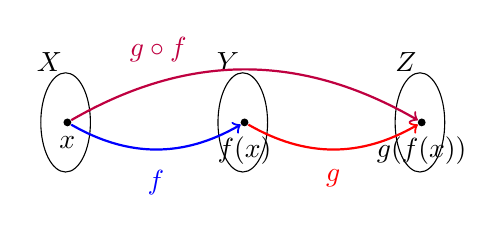
\begin{tikzpicture}[scale=0.45]
		\draw \boundellipse{0,0}{0.7}{1.4};
		\draw\boundellipse{5,0}{0.7}{1.4};
		\draw\boundellipse{10,0}{0.7}{1.4};
		\node at (0.45,1.7) [label=left:$X$]{};
		\node at (5.45,1.7) [label=left:$Y$]{}; 
		\node at (10.45,1.7) [label=left:$Z$]{}; 
		\node[circle, fill,inner sep=1pt] (x) at (0.05,0) [label=below:$x$]{};
		\node[circle, fill,inner sep=1pt] (fx) at (5.05,0) [label=below:$f(x)$]{};
		\node[circle, fill,inner sep=1pt] (gfx) at (10.05,0) [label=below:$g(f(x))$]{};
		\draw[thick,->,blue] (x) to [bend right] node[pos=0.5, label=below:$f$] {} (fx) ;
		\draw[thick,->,red] (fx) to [bend right] node[pos=0.5, label=below:$g$] {} (gfx) ;
		\draw[thick,->,purple] (x) to [bend left] node[pos=0.25, label=above:$g\circ f$] {} (gfx) ;
\end{tikzpicture}%
\end{center}
\subsection{Inverse funktioner}
To funktioner $f\colon X\to Y$ og $g\colon Y\to X$ er hinandens \emph{inverse} hvis
\begin{align*}
f(g(y))=y,\quad \textup{og}\quad g(f(x))=x 
\end{align*}
for alle $x$ i $X$ og $y$ i $Y$.

\begin{center}
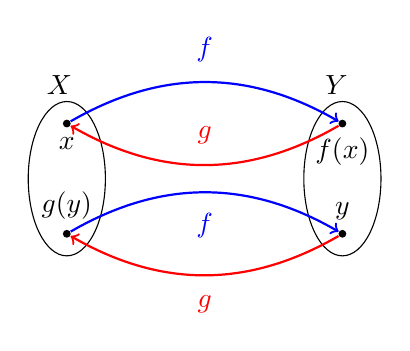
\begin{tikzpicture}[scale=0.7]
\draw \boundellipse{0,0}{0.7}{1.4};
\draw \boundellipse{5,0}{0.7}{1.4};
\node at (0.45,1.7) [label=left:$X$]{};
\node at (5.45,1.7) [label=left:$Y$]{}; 
\node[circle,fill,inner sep=1pt] (x) at (0,1) [label=below:$x$] {};
\node[circle,fill,inner sep=1pt] (gy) at (0,-1) [label=above:$g(y)$] {};
\node[circle,fill,inner sep=1pt] (fx) at (5,1) [label=below:$f(x)$] {};
\node[circle,fill,inner sep=1pt] (y) at (5,-1) [label=above:$y$] {};
\draw[thick,->,blue] (x) to[bend left]node[pos =0.5, label=above:$f$] {} (fx);
\draw[thick,->,red] (fx) to[bend left] node[pos =0.5, label=above:$g$] {} (x);
\draw[thick,->,red] (y) to[bend left]node[pos =0.5, label=below: $g$] {} (gy);
\draw[thick,->,blue] (gy) to[bend left]node[pos =0.5, label=below: $f$] {} (y);
\end{tikzpicture}%
\end{center}

\subsection{Polynomier}
Et førstegradspolynomium har forskrift:
\begin{align*}
f(x)=ax+b.
\end{align*}
Et andengradspolynomium har forskrift:
\begin{align*}
f(x)=ax^2+bx+c.
\end{align*}
\subsection{Logaritmer og eksponentialfunktioner}
\emph{Logaritmen med grundtal $a$}, $\log_a\colon ]0,\infty[\to \R$ er invers til eksponentialfunkionen $f_a(x)=a^x$ ($a>0$, $a\neq 1$). Der gælder at
\begin{align*}
\log_a(a^x)=x\quad \textup{og} \quad a^{\log_a(y)}=y
\end{align*}
og vi har
\begin{align*}
\ln x=\log_e x,&& \log x=\log_{10} x
\end{align*}
\subsection{Regneregler}
Der gælder
\begin{align*}
\log_a(xy)&=\log_a(x)+\log_a(y),\\\log_a\Big(\frac{x}{y}\Big)&=\log_a(x)-\log_a(y),\\ \log_a(x^r)&=r\log_a(x).
\end{align*}
\section{Trigonometriske funktioner}
De trigonometriske funkioner er defineret ud fra enhedscirklen:
\begin{center}
	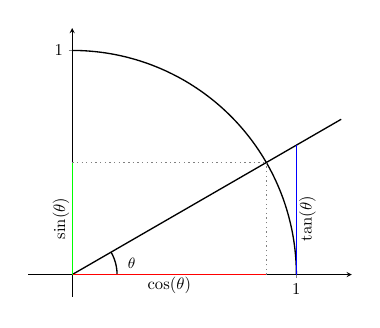
\begin{tikzpicture}[scale=0.6]
	\begin{axis}[xmin=-0.05,xmax=1.1,ymin=-0.1,ymax=1.1,axis x line=center,
	axis y line=center, axis equal, xtick={0,1},ytick={0,1}]
	%PERMANENT STUFF
	\addplot[domain=0:pi/2,thick, samples=100] ({cos(deg(x))},{sin(deg(x))});
	\addplot[domain=0:sqrt(3)/2,thick] {1/sqrt(3)*x};
	\addplot[domain=0:pi/6,thick,samples=100] ({0.2*cos(deg(x))},{0.2*sin(deg(x))}) node[label=right:{\small$\theta$},pos=0.5] {};
	%cos
	\addplot[dotted,gray,thick] coordinates {(sqrt(3)/2,0) (sqrt(3)/2, 1/2)};
	\node at (axis cs: {sqrt(3)/4},-0.05) {$\cos(\theta)$};
	\addplot[thick,red,domain=0:sqrt(3)/2] {0};
	%sin
	\node at (axis cs: -0.05,1/4) {\rotatebox{90}{$\sin(\theta)$}};
	\addplot[dotted, gray,thick,domain=0:sqrt(3)/2] {1/2};	
	\addplot[thick,green]  coordinates { (0,0) (0,1/2)};
	%tan
	\addplot[thick,domain=sqrt(3)/2:1.2] {1/sqrt(3)*x};
	\node at (axis cs: 1.05,1/4) {\rotatebox{90}{$\tan(\theta)$}};
	\addplot[blue,thick] coordinates {(1,0) (1, 1/sqrt(3)};
	\end{axis}
	\end{tikzpicture}%
\end{center}
Der gælder at
\begin{center}
\begin{tabular}{@{} lccccc @{}}
	\toprule 
	$\theta$			& 0			&$ \frac{\pi}{6} $  		&$ \frac{\pi}{4} $ 		&$ \frac{\pi}{3}$ 			&$ \frac{\pi}{2} $		\\ \midrule
	$\sin \theta$		&0			&$ \frac{1}{2} $			&$ \frac{\sqrt{2}}{2} $	& $ \frac{\sqrt{3}}{2} $ 	& 1						\\ \midrule
	$\cos \theta$		&1			&$\frac{\sqrt{3}}{2}$		&$\frac{\sqrt{2}}{2}$	& $\frac{1}{2}$				&0	\\ \midrule
	$\tan \theta$		&0			&$\frac{1}{\sqrt{3}}$		&$1$					& $ \sqrt{3} $				&-		\\ \midrule
\end{tabular}
\end{center}
samt $ \tan(\theta)=\frac{\sin(\theta)}{\cos(\theta)}$.





%\begin{tabular}{@{} lccc @{}}
%	\toprule 
%	$\theta$			& $\sin \theta$			& $\cos \theta$ 		& $\tan \theta$ 		\\ \midrule
%	0					&0						&1						&0						\\ \midrule
%	$ \frac{\pi}{6} $	&$\frac{1}{2}$			&$\frac{\sqrt{3}}{2}$	&$\frac{1}{\sqrt{3}}$	\\ \midrule
%	$ \frac{\pi}{4} $	&$\frac{\sqrt{2}}{2}$	&$\frac{\sqrt{2}}{2}$	&$1$					\\ \midrule
%	$ \frac{\pi}{3} $	&$\frac{\sqrt{3}}{2}$	&$\frac{1}{2}$			&$\sqrt{3}$				\\ \midrule
%	$ \frac{\pi}{2} $	&1						&0						&						\\ \bottomrule  
%\end{tabular}


















        \section{Derivatives}
The derivative of $f$ is denoted $f'=\frac{d}{dx}f=\frac{df}{dx}$.

\textcolor{white}{hemmelig tekst}

\subsection{Rules}
We have that
\begin{center}
		\begin{tabular}{@{}l l@{}}
		$f(x)$      & $f'(x)$  				\\ \toprule
		$c$			& $0$ 					\\ \midrule
		$x$			& $1$					\\ \midrule
		$x^n$  		& $nx^{n-1}$			\\ \midrule
		$e^x$  		& $e^x$					\\ \midrule
		$e^{cx}$  	& $ce^{cx}$				\\ \midrule
		$a^x$  		& $a^x\ln a $			\\ \midrule
		$\ln x$ 	& $\frac{1}{x}$			\\ \midrule
		$\cos x$  	& $-\sin x$				\\ \midrule
		$\sin x$  	& $\cos x$				\\ \midrule
		$\tan x$ 	& $1+\tan^2(x)$		\\ \bottomrule  
	\end{tabular}
\end{center}
\subsection{General Rules}
We have that
\begin{align*}
&(cf)'(x)=cf'(x)\\
&(f\pm g)'(x)=f'(x)\pm g'(x)\\
&(fg)'(x)=f'(x)g(x)+f(x)g'(x)\\
&\Big(\frac{f}{g}\Big)'(x)=\frac{f'(x)g(x)-f(x)g'(x)}{g^2(x)}\\
&\frac{d}{dx}f(g(x))=f'(g(x))g'(x).
\end{align*}
The last formula is also called the \emph{chain rule}.
        \section{Ubestemte integraler}
En funktion $f$ har \emph{stamfunktion} $F$ hvis
\begin{align*}
F'(x)=f(x).
\end{align*}
Det ubestemte integral af $f$ defineres til
\begin{align*}
\int f(x)\, dx =F(x)+k,
\end{align*}
hvor $F$ er en stamfunktion til $f$ og $k\in \R$.
\subsection{Generelle regneregler}
\begin{align*}
&\int cf(x) \, d x=c\int f(x)\, dx\\
&\int f(x)\pm g(x) \, d x=\int f(x)\, dx\pm \int g(x) \, dx.\\
&\int f(x)g(x)\, dx=f(x)G(x)-\int f'(x)G(x)\, dx\\
&\int f(g(x))g'(x)\, dx =F(g(x))+k.
\end{align*}
Den 3. regel kaldes \emph{delvis integration} og den sidste kaldes \emph{integration ved substitution}.
\subsection{Regneregler}
Der gælder at
\begin{center}
		\begin{tabular}{@{}l l@{}}
		$f(x)$      & $\int f(x)\, dx$  				\\ \toprule
		$c$			& $cx+k$ 							\\ \midrule
		$x$			& $\frac{1}{2}x^2+k$				\\ \midrule
		$x^n$  		& $\frac{1}{n+1}x^{n+1}+k$			\\ \midrule
		$e^x$  		& $e^x+k$							\\ \midrule
		$e^{cx}$  	& $\frac{1}{c}e^{cx}+k$				\\ \midrule
		$\frac{1}{x}$ & $\ln(\vert x\vert)+k $			\\ \midrule
		$\ln x$ 	& $x\ln(x)-x+k$						\\ \midrule
		$\cos x$  	& $\sin x+k$						\\ \midrule
		$\sin x$  	& $-\cos x+k$						\\ \midrule
		$\tan x$ 	& $-\ln(\vert \cos(x)\vert)+k$		\\ \bottomrule  
	\end{tabular}
\end{center}
\subsection{Integration ved substitution}
Givet et integral på formen $\int f(g(x))g'(x)\, dx$ anvendes metoden:
\begin{enumerate}
	\item Lad $u=g(x)$.
	\item Udregn $\frac{du}{dx}$ og isoler $dx$.
	\item Substituer $g(x)$ og $dx$.
	\item Udregn integralet mht. $u$.
	\item Substituer tilbage.
\end{enumerate}
\section{Besemte integraler}
Det bestemte integral af $f$ i intervallet $[a,b]$ til
\begin{align*}
\int_a^b f(x)\, dx =[F(x)]_a^b=F(b)-F(a),
\end{align*}
hvor $F$ er en stamfunktion til $f$.
\subsection{Generelle regneregler}
\begin{align*}
&\int_a^b cf(x) \, d x=c\int_a^b f(x)\, dx\\
&\int_a^b \!\!f(x)\pm g(x) \, d x=\int_a^b\!\!f(x)\, dx\pm \int_a^b\!\! g(x) \, dx\\
&\int_a^b\!\!\! \!\!\!f(x)g(x)\, dx\!\!=\!\![f(x)G(x)]_a^b\!\!-\!\!\!\!\int_a^b\!\!\!\!\!\! f'(x)G(x)\, dx\\
%&\phantom{\int_a^b f(x)g(x)\, dx=}-\int_a^b f'(x)G(x)\, dx\\
&\int_a^b f(g(x))g'(x) \, dx=[F(x)]_{g(a)}^{g(b)}.
\end{align*}
\subsection{Integration ved substitution}
Givet et integral på formen $\int_a^b f(g(x))g'(x)\, dx$ anvendes metoden
	\begin{enumerate}
	\item Lad $u=g(x)$.
	\item Udregn $\frac{du}{dx}$ og isoler $dx$.
	\item Substituer $g(x)$, $dx$ samt grænser.
	\item Udregn integralet mht. $u$.
\end{enumerate}
        \mysection{Differentialligninger}


\mysubsection{Løsningsformler}
\begin{center}
\begin{tabular}{@{}l l@{}}
Differentiallign.    & Fuldstændig løsn.				\\ \toprule
$f'(x)=k$				& $f(x)=kx+c$						\\ \midrule
$f'(x)=h(x)$			& $f(x)=\int h(x) \d x$				\\ \midrule
$f'(x)=kf(x)$			& $f(x)=ce^{kx}$					\\ \midrule
$f'(x)+ af(x) =b$		& $f(x)=\frac{b}{a}+ce^{-ax}$		\\ \bottomrule  
\end{tabular}
\end{center}

\mysubsection{Panserformlen}
Differentialligningen 
\begin{equation*}
f'(x)+a(x)f(x)=b(x)
\end{equation*}
har fuldstændig løsning
\begin{equation*}
f(x)=e^{-A(x)}\int b(x) e^{A(x)}dx +ce^{-A(x)},
\end{equation*}
hvor $A'(x)=a(x)$.
        \mysection{Vektorer i planen}
En vektor $\vec{u}$ i planen skrives som $\vec{u}=[x,y]$ hvor $x,y\in \R$.
\mysubsection{Regneregler}
For $\vec{u}=[x_1,y_1]$, $\vec{v}=[x_2,y_2]$, $c\in \R$ er 
\begin{align*}
    \vec{u}\pm\vec{v}=\begin{bmatrix}
        x_1\pm x_2\\y_1\pm y_2
    \end{bmatrix}, &&\vec{u}\cdot\vec{v}=x_1x_2+y_1y_2 ,\\
    c\vec{u}=\begin{bmatrix*}
        cx_1\\cy_1
    \end{bmatrix*}, && \!\!\!\det(\vec{u},\vec{v})=x_1y_2-x_2y_1
\end{align*}
Længden af $\vec{u}$ er $\left\Vert \vec{u}\right\Vert=\sqrt{x_1^2+y_1^2}$.
\mysubsection{Vinklen mellem to vektorer}
For vinklen $\theta$ mellem $\vec{u}$, $\vec{v}$ er 
\begin{align*}
    \cos\theta=\frac{\vec{u}\cdot\vec{v}}{\left\Vert \vec{u}\right\Vert \left\Vert \vec{v}\right\Vert }, && \sin\theta=\frac{\det(\vec{u},\vec{v})}{\left\Vert \vec{u}\right\Vert \left\Vert \vec{v}\right\Vert}
\end{align*}
Yderligere gælder 
\begin{enumerate}
    \item $\vec{u}$ og $\vec{v}$ er ortogonale $\Leftrightarrow $ $\vec{u}\cdot\vec{v}=0$.
    \item $\vec{u}$ og $\vec{v}$ er parallelle $\Leftrightarrow$ $\det(\vec{u},\vec{v})=0$.
\end{enumerate}
\
\mysection{Vektorer i rummet}
En vektor $\vec{u}$ i rummet skrives som $\vec{u}=[x,y,z]$ hvor $x,y,z\in \R$.
\mysubsection{Regneregler}
For $\vec{u}=[x_1,y_1,z_1]$, $\vec{v}=[x_2,y_2,z_2]$ og $c\in \R$ gælder 
\begin{align*}
    &\vec{u}\pm\vec{v}=\begin{bmatrix}
        x_1\pm x_2\\y_1\pm y_2\\z_1\pm z_2
    \end{bmatrix}, && c\vec{u}=\begin{bmatrix*}
        cx_1\\cy_1\\c z_1
    \end{bmatrix*},\\
    &\vec{u}\cdot\vec{v}=x_1x_2+y_1y_2+z_1z_2. &&
\end{align*}
Længden af $\vec{u}$ er $\left\Vert \vec{u}\right\Vert=\sqrt{x_1^2+y_1^2+z_1^2}$. Krydsproduktet er givet ved 
\begin{equation*}
    \vec{u}\times \vec{v}=\begin{bmatrix}
        y_1z_2-z_1y_2\\ z_1x_2-x_1z_2\\x_1y_2-y_1x_2
    \end{bmatrix}
\end{equation*}
\mysubsection{Vinklen mellem to vektorer}
For vinklen $\theta$ mellem $\vec{u}$ og $\vec{v}$ gælder 
\begin{align*}
    \cos\theta=\frac{\vec{u}\cdot\vec{v}}{\left\Vert \vec{u}\right\Vert \left\Vert \vec{v}\right\Vert }, && \sin\theta=\frac{\left\Vert \vec{u}\times \vec{v}\right\Vert }{\left\Vert \vec{u}\right\Vert \left\Vert \vec{v}\right\Vert}
\end{align*}
Yderligere gælder 
\begin{enumerate}
    \item $\vec{u}$ og $\vec{v}$ er ortogonale $\Leftrightarrow$ $\vec{u}\cdot\vec{v}=0$.
    \item $\vec{u}$ og $\vec{v}$ er parallelle $\Leftrightarrow$ $\vec{u}\times\vec{v}=0$.
\end{enumerate}
\mysection{Linjer og Planer}
Planen/linjen gennem punktet med stedvektor $\vec{x}_0$ med normalvektor $\vec{n}$ beskrives ved alle vektorer $\vec{x}$ der løser ligningen
\begin{equation*}
    \vec{n}\cdot(\vec{x}-\vec{x_0})=0
\end{equation*}
En linje i rummet/planen gennem punktet med stedvektor $\vec{x}_0$ og retning $\vec{r}$ har parameterfremstilling
\begin{align*}
    \vec{x}_0+t\vec{r}, \quad t\in \R.
\end{align*}
    \end{multicols*}
    }
\restoregeometry
\addtocontents{toc}{\protect\setcounter{tocdepth}{1}}
\chapter{Basal matematik}
\section{Brøker}
\noindent Når vi snakker om brøker tænker vi på tal på formen
\begin{align*}
\textup{brøk } = \frac{\textup{ tæller }}{ \textup{ nævner }},
\end{align*}
hvor det eneste krav er at nævneren ikke må være $0$. 

Vi vil ofte skrive en brøk som
\begin{align*}
a=\frac{b}{c},
\end{align*}
hvor $b$ kan være et hvilket som helst tal og $c$ kan være alle tal bortset fra $0$.

Det kan f.eks. være $5$ venner der vælger at dele en pizza ligeligt imellem sig, så de får $\frac{1}{5}$ hver, eller $3$ venner der har tjent 200 kr og hver især får $\frac{200}{3}$ kr.

\paragraph*{Størrelsesforhold:} 
Der gælder at hvis nævneren i en brøk er større end tælleren, så er brøken mindre end $1$, f.eks. $\frac{1}{2} < 1$. Hvis nævneren er lig med tælleren så er brøken lig med $1$, f.eks. $\frac{4}{4}=1$ og hvis nævneren er mindre end tælleren så er brøken større end $1$, f.eks. $\frac{4}{3} > 1$.

En anden måde vi kan skrive dette på er:
\begin{align*}
&\frac{a}{b} < 1, \quad \textup{ hvis }a < b,\\
&\frac{a}{b} = 1, \quad \textup{ hvis }a = b,\\
&\frac{a}{b} > 1, \quad \textup{ hvis }a > b.
\end{align*}
Derudover gælder der, at hvis man gør nævneren større så får man en mindre brøk, eksempelvis $\frac{2}{3} > \frac{2}{5}$, hvorimod hvis man gør tælleren større så får man en større brøk, som i tilfældet $\frac{3}{4} < \frac{7}{4}$.

Igen kan vi skrive dette mere præcist ved:
\begin{align*}
\frac{a}{b} < \frac{a}{c}, \quad \textup{ hvis }c < b,\\
\frac{a}{b} < \frac{c}{b}, \quad \textup{ hvis }a < c.
\end{align*}

\paragraph*{Regneregler:}
Det er ekstremt vigtigt at man lærer de følgende regneregler for brøker, da de vil dukke op igen og igen resten af kurset og i jeres videre studieforløb.
\begin{enumerate}
\item Når vi lægger to brøker sammen eller trækker dem fra hinanden, finder vi først fælles nævner og derefter lægger vi tællerne sammen eller trækker dem fra hinanden. 

En måde at finde fælles nævner, som altid virker, er at gange på kryds:
\begin{align*}
\frac{a}{b}\pm \frac{c}{d}= \frac{a \cdot d}{b \cdot d} \pm \frac{b \cdot c}{b \cdot d} = \frac{a \cdot d \pm b \cdot c}{b \cdot d}.
\end{align*}
\item Når vi ganger et tal med en brøk, ganger vi tallet op i tælleren:
\begin{align*}
a \cdot \frac{b}{c}=\frac{a \cdot b}{c}.
\end{align*}
\item Når vi dividerer en brøk med et tal, ganger vi tallet ned i nævneren:
\begin{align*}
\frac{\frac{a}{b}}{c}=\frac{a}{b\cdot c}.
\end{align*}
Bemærk, at brøkstregen i den brøk der står i tælleren er mindre end den anden brøkstreg. Grunden til det er at så kan vi se forskel på om vi dividere en brøk med et tal eller et tal med en brøk. 
\item Når vi dividerer et tal med en brøk, ganger vi tallet på den omvendte brøk:
\begin{align*}
\frac{a}{\frac{b}{c}}= a \cdot \frac{c}{b} = \frac{a \cdot c}{b}.
\end{align*}
Bemærk, at når vi siger den omvendte brøk af $\frac{a}{b}$ så mener vi brøken $\frac{b}{a}$, hvor vi har byttet om på tæller og nævner.
\item Når vi ganger to brøker sammen, ganger vi tæller med tæller og nævner med nævner:
\begin{align*}
\frac{a}{b} \cdot \frac{c}{d} = \frac{a \cdot c}{b \cdot d}
\end{align*}
\item Når vi dividerer en brøk med en brøk, ganger vi med den omvendte brøk:
\begin{align*}
\frac{\frac{a}{b}}{\frac{c}{d}} = \frac{a}{b} \cdot \frac{d}{c} = \frac{a \cdot d}{b \cdot c}.
\end{align*}
\end{enumerate}
Det er ofte nemmere at forstå regnereglerne hvis man ser nogle konkrete eksempler.
\paragraph*{Eksempler:}
\begin{enumerate}
\item Udregn $\frac{4}{5}-\frac{2}{3}$:
\begin{align*}
\frac{4}{5}-\frac{2}{3} = \frac{4\cdot 3}{5 \cdot 3} - \frac{5 \cdot 2}{5 \cdot 3} = \frac{12}{15} - \frac{10}{15} = \frac{12-10}{15} = \frac{2}{15}.
\end{align*}
\item Udregn $2 \cdot \frac{4}{5}$:
\begin{align*}
2 \cdot \frac{4}{5}= \frac{2 \cdot 4}{5} = \frac{8}{5}.
\end{align*}
\item Udregn $\frac{\frac{4}{3}}{7}$:
\begin{align*}
\frac{\frac{4}{3}}{7} = \frac{4}{3 \cdot 7} = \frac{4}{21}.
\end{align*}
\item Udregn $\frac{5}{\frac{2}{3}}$:
\begin{align*}
\frac{5}{\frac{2}{3}} = 5 \cdot \frac{3}{2} = \frac{5 \cdot 3}{2} = \frac{15}{2}.
\end{align*}
\item Udregn $\frac{3}{4} \cdot \frac{9}{4}$:
\begin{align*}
\frac{3}{4} \cdot \frac{9}{4} = \frac{3 \cdot 9}{4 \cdot 4} = \frac{27}{16}.
\end{align*}
\item  Udregn $\frac{\frac{1}{2}}{\frac{3}{5}}$:
\begin{align*}
\frac{\frac{1}{2}}{\frac{3}{5}} = \frac{1}{2} \cdot \frac{5}{3} = \frac{1 \cdot 5}{2 \cdot 3} = \frac{5}{6}.
\end{align*}
\end{enumerate}

\paragraph*{Forlænge og forkorte brøker:}
Et trick i matematikken er at tage et tal og gange det med $1$, da det ikke ændre noget ved det oprindelige tal, men hvis man skriver $1$ på en smart måde kan det ofte simplificere ens udregninger. 

Hvis vi ganger en brøk med $a$ i både tæller og nævner kalder vi det at \emph{forlænge brøken med $a$}:
\begin{align*}
\frac{b}{c} = \frac{b}{c} \cdot 1 = \frac{b}{c} \cdot \frac{a}{a} = \frac{b \cdot a}{c \cdot a}.
\end{align*}
Hvis vi dividere en brøk med $a$ i både tæller og nævner så kalder vi det at \emph{forkorte brøken med $a$}:
\begin{align*}
\frac{b}{c} \cdot 1 = \frac{b}{c} \cdot \frac{\frac{1}{a}}{\frac{1}{a}} = \frac{\frac{b}{a}}{\frac{c}{a}}. 
\end{align*}
Bemærk at ved at forlænge eller forkorte brøker, ændre vi ikke deres værdi.
\paragraph{Eksempler:}
\begin{enumerate}
\item Forlæng brøken $\frac{4}{5}$ med $2$:
\begin{align*}
\frac{4}{5} \cdot 1 = \frac{4}{5} \cdot \frac{2}{2} = \frac{4 \cdot 2}{5 \cdot 2} = \frac{8}{10}.
\end{align*}
\item Forkort brøken $\frac{8}{10}$ med $2$:
\begin{align*}
\frac{8}{10} \cdot 1 = \frac{8}{10} \cdot  \frac{\frac{1}{2}}{\frac{1}{2}} = \frac{\frac{8}{2}}{\frac{10}{2}} = \frac{4}{5}.
\end{align*}
\end{enumerate}
Bemærk at dette betyder, at når vi forkorter en brøk med $a$ dividerer vi samtlige led i både tæller og nævner med $a$. Det er en klassisk fejl som mange begår, at man tror man kan nøjes med at forkorte nogle af leddene i tælleren eller nævneren, f.eks. er
\begin{align*}
\frac{x^3+x^2+1}{x} \neq x^2+x+1,
\end{align*} 
da $x$ ikke går op i $1$. Det rigtige vil i stedet være at forkorte brøken med $x$, hvilket giver
\begin{align*}
\frac{x^3+x^2+1}{x}= \frac{\frac{x^3}{x}+\frac{x^2}{x}+ \frac{1}{x}}{\frac{x}{x}} = x^2+x+\frac{1}{x}.
\end{align*}

Vi siger at en brøk er \emph{uforkortelig} hvis der ikke eksisterer noget heltal større end $1$, som går op i både tælleren og nævneren. 

Alle facit i dette kursus, som er brøker, skal angives som uforkortelige brøker (ikke decimaltal), eksempelvis:
\begin{align*}
\frac{2}{4}+\frac{8}{4} = \frac{10}{4} = \frac{5}{2},
\end{align*}
har facit $\frac{5}{2}$ og ikke $\frac{10}{4}$, selvom tallene i princippet et ens. 














\subsection{Opgaver}

\begin{enumerate}
\item Omskriv følgende tal til brøker hvor nævneren er 4:
\begin{align*}
2,&& \iffalse 5,&&  \frac{4}{8},&& \fi \frac{60}{24},&& \pi,&& \frac{3}{2}.% ,&& \frac{12}{16},&&30.
\end{align*}
\item Omskriv følgende tal til brøker hvor nævneren er 3:
\begin{align*}
7,&& \iffalse 3,&&\frac{2}{6},&& \fi \frac{6}{9},&&\frac{16}{12},&&4\pi.% && \frac{14}{21},&&e.
\end{align*}
\item Udregn følgende tal (forkort mest muligt):
\begin{align*}
\frac{6}{7}+\frac{8}{7},&& \frac{1}{2}+\frac{3}{4},&& \frac{1}{2}+\frac{1}{3}+\frac{1}{4},&& \frac{3}{2}-\frac{4}{8},&&-\frac{2}{3}+\frac{2}{6}.
\end{align*}
\item Udregn følgende tal (forkort mest muligt):
\begin{align*}
2\c\frac{3}{4},&&\frac{1}{8}\c \frac{2}{3},&& \frac{7}{8}\c \frac{1}{3},&& 2\c3\c \frac{1}{4}\c\frac{1}{5},&&\frac{2}{3}\c \frac{7}{3},&&\frac{3}{5}\c \frac{15}{25}.
\end{align*}
\item Udregn følgende tal (forkort mest muligt):
\begin{align*}
\frac{6}{ \frac{3}{2}},&& \frac{ \frac{2}{3}}{ \frac{4}{9}},&& \frac{ \frac{3}{2}}{6},&& \frac{ \frac{2}{7}}{ \frac{14}{49}},&& \frac{ (\frac{1}{2}:\frac{3}{4})}{ \frac{8}{15}}.
\end{align*}
\item Forkort følgende brøker mest muligt:
\begin{align*}
\frac{x^2+x}{x},&& \frac{2x+4y}{2},&& \frac{2xy+7y}{y},&&\frac{x^2y+xy}{x(x+1)},&& \frac{(x+3)^2}{2x^2+6x},&& \frac{2 (x-1)^2}{6x^2-6x}.
\end{align*}
\item Udregn følgende tal (forkort mest muligt):
\begin{align*}
\frac{3}{2}-\bigg(\frac{1}{5}\c \frac{2}{10}\bigg),&& -21\bigg( \frac{2}{3}- \frac{1}{7}\bigg),&& \frac{2}{4}\c \frac{8}{4}-\frac{3}{8},&& \frac{\frac{2}{5}}{3}-2\c \frac{2}{30},&& \frac{6}{ \frac{2}{3}} +\frac{1}{2}.
\end{align*}
\item Reducer følgende brøk mest muligt:
\begin{align*}
\frac{a-(2b-9)}{a-2b}-\frac{a-(b-5)}{a-2b}+\frac{a-(b+4)}{a-2b}.
\end{align*}
\item Indsæt det tal som mangler:
\begin{align*}
\frac{1}{2}= \frac{3}{},&& \frac{6}{7}=\frac{}{49},&& \frac{2x}{y}=\frac{2xy}{},&& \frac{ \pi}{\sqrt{2}}=\frac{}{3 \pi^2 \sqrt{2}}.
\end{align*}
\item Udregn følgende tal (forkort mest muligt):
\begin{align*}
\frac{ \frac{1}{2}+\frac{2}{5}}{1+\frac{1}{10}},&& \frac{ \frac{3}{4}+1}{ \frac{9}{8}-1},&& \frac{2}{3}\c \frac{ \frac{5}{2}-2}{ \frac{8}{3}+1}.
\end{align*}
\item Reducer følgende brøk:
\begin{align*}
\frac{4a+(2c-4b)}{a-b} - (c-2)-\frac{2c-ac+bc}{a-b}.
\end{align*}
\item Vis, at
\begin{align*}
\frac{ \frac{1}{b}+1 }{1- \frac{a}{b}}=\frac{1+b}{b-a},
\end{align*}
hvor $b\notin \{0,a\}$.
\item Vis at
\begin{align*}
\frac{ \frac{a}{b}+1}{ \frac{b}{a}+1}=\frac{a}{b},
\end{align*}
hvor $a,b\neq 0$ og $a\neq -b$. Hvorfor kræver vi at $a,b\neq 0$ samt at $a\neq -b$?
\end{enumerate}


\section{Kvadratsætninger}
\noindent Hvis vi har et udtryk som vi gerne vil reducere, møder vi ofte noget på formen $(a+b)^2$. For at komme videre i vores udregning vil vi derfor gerne kunne omskrive sådanne udtryk så de bliver nemmere at reducere. Til at gøre dette introducerer vi kvadratsætningerne.

Vi husker at når vi ganger to parenteser sammen, så benytter vi følgende formel
\begin{align*}
(a+b)(c+d)=ac+ad+bc+bd,
\end{align*}
som vi får ved først at gange $a$ ind på begge elementer i den anden parentes og dernæst gange $b$ ind på de to elementer.

Hvis vi bruger denne regneregel får vi:
\begin{align*}
&(a+b)^2=(a+b)(a+b)=a^2+ab+ba+b^2=a^2+b^2+2ab \\
&(a-b)^2=(a-b)(a-b)=a^2-ab-ba+(-b)^2 = a^2+b^2-2ab\\
&(a+b)(a-b)=a^2-ab+ba-b^2 = a^2-b^2.
\end{align*}
Bemærk her, at $(-b)^2 \neq -b^2$ medmindre $b=0$, da $(-b)^2 = (-b)\cdot (-b)=(-1)\cdot b \cdot (-1) \cdot b = (-1)^2 \cdot b^2 = b^2$ og $-b^2 = (-1) \cdot b^2$.

Det giver os de tre kvadratsætninger, som kort kan skrives:
\begin{enumerate}
\item $(a+b)^2=a^2+b^2+2ab$.
\item $(a-b)^2=a^2+b^2-2ab$.
\item $(a+b)(a-b)=a^2-b^2$.
\end{enumerate}

\paragraph{Eksempler:}
\begin{enumerate}
\item Reducer $(x+y)^2+(x-y)^2-x^2-y^2$:
\begin{align*}
(x+y)^2+(x-y)^2-x^2-y^2 &= x^2+y^2+2xy + x^2+y^2-2xy - x^2-y^2 \\
&=x^2+y^2.
\end{align*}
\item Reducer $\frac{1}{a+b}+\frac{1}{a-b}$:

Ved at benytte brøkregnereglerne fra sidste kursusgang får vi
\begin{align*}
\frac{1}{a+b}+\frac{1}{a-b} &= \frac{a-b}{(a+b)(a-b)} + \frac{a+b}{(a+b)(a-b)} \\
&= \frac{a-b+a+b}{(a+b)(a-b)} \\
&=\frac{2a}{a^2-b^2}.
\end{align*}
\item Reducer $\frac{2x^2+2-4x}{2x^2-2}$:

Vi ser ved hjælp af vores kvadratsætninger at
\begin{align*}
&2x^2+2-4x = 2(x^2+1-2x) = 2 (x-1)^2 \\
&2x^2-2 = 2(x^2-1) = 2(x-1)(x+1).
\end{align*}
Hvis vi indsætter dette og reducere, får vi
\begin{align*}
\frac{2x^2+2-4x}{2x^2-2} = \frac{2 (x-1)^2}{2(x-1)(x+1)} = \frac{x-1}{x+1}.
\end{align*}
\end{enumerate}

\paragraph*{Afstandsformlen:} Vi husker Pythagoras Sætning der siger at for en retvinklet trekant med sidelængderne $a,b,c$ hvor $c$ er hypotenusen, gælder der:
\begin{align*}
a^2+b^2=c^2.
\end{align*}
Ved at benytte Pythagoras Sætning får vi at afstanden $c$ mellem to punkter $P$ og $Q$ i et koordinatsystem som i Figur~\ref{fig:1lec} 
\begin{figure}[!htbp]
  \pgfplotsset{width=0.5\textwidth,compat=1.11}
  \centering
  \begin{tikzpicture}
  \begin{axis}[ 
    xmin=-0.1,
    xmax=2.7,
    ymin=0.5,
    ymax=1.7,
    axis equal,
    %axis lines=middle,
 ticks=none,
xlabel={},
ylabel={},
  ]
\node[circle,fill,inner sep=0pt,minimum size=3pt] (P) at (1,0.5) {};
\node[below,left] at (1,0.5) {$P=(x_1,y_1)$};
\node[circle,fill,inner sep=0pt,minimum size=3pt] (Q) at (2,1.5) {};
\node[above] at (2,1.5) {$Q=(x_2,y_2)$};
\node[circle,fill,inner sep=0pt,minimum size=3pt] (R) at (2,0.5) {};
\draw (P)--(Q);
\draw[dashed] (P)--(R)--(Q);
\node[below] at (1.5,0.5) {$x_2-x_1$};
\node[right] at (2,1) {$y_2-y_1$};
%\draw (1,1) circle [radius =sqrt(2)]; 
\end{axis}
 \end{tikzpicture}
  \caption{Afstanden mellem $P$ og $Q$.}
  \label{fig:1lec}
\end{figure}
er givet ved
\begin{align*}
(x_2-x_1)^2+(y_2-y_1)^2=c^2.
\end{align*}

\paragraph{Cirklens ligning:}
Ved at bruge afstandsformlen kan vi nu opstille en ligning for en cirkel med centrum i punktet $(a,b)$ og med radius $r$, som i Figur~\ref{fig:2lec}.
\begin{figure}[!htbp]
  \pgfplotsset{width=0.5\textwidth,compat=1.11}
  \centering
  \begin{tikzpicture}
  \begin{axis}[ xmin=-0.1,
    xmax=2.5,
    ymin=-1.3,
    ymax=2.5,
   axis equal,
    axis lines=middle,
 ticks=none,
xlabel={},
ylabel={},
  ]
\node[circle,fill,inner sep=0pt,minimum size=3pt] (P) at (1,0.5) {};
\node[below,left] at (1,0.5) {$(a,b)$};
\node[circle,fill,inner sep=0pt,minimum size=3pt] (Q) at (2,1.5) {};
\node[above,right] at (2,1.5) {$(x,y)$};
\node[circle,fill,inner sep=0pt,minimum size=3pt] (R) at (2,0.5) {};
\draw (P)--(Q);
\draw[dashed] (P)--(R)--(Q);
\node[above,left] at (1.4,1.1) {$r$};
\draw (1,0.5) circle [radius =sqrt(2)]; 
\end{axis}
 \end{tikzpicture}
  \caption{Cirklens ligning.}
  \label{fig:2lec}
\end{figure}
Alle punkterne der ligger på denne cirkel vil opfylde at deres afstand til punktet $(a,b)$ er $r$. Dette kan vi ved hjælp af afstandsformlen skrive som en ligning givet ved
\begin{align*}
(x-a)^2+(y-b)^2=r^2,
\end{align*}
hvor $(x,y)$ er punkter på cirklen. Denne ligning kaldes for \emph{cirklens ligning}.

\paragraph*{Eksempler:}
\begin{enumerate}
\item Find cirklens ligning for en cirkel med centrum i $(2,3)$ med radius $r=4$:

Vi indsætter $(2,3)$ og $r=4$ i cirklens ligning og reducere
\begin{align*}
(x-2)^2+(y-3)^2=16.
\end{align*}
\item Find centrum og radius for en cirkel med ligning $x^2-4x+y^2-2y=-4$:

For a omskrive ligningen til noget på samme form som cirklens ligning vil vi bruge kvadratsætningerne den modsatte vej af hvad vi har gjort indtil nu. Vi ser at 
\begin{align*}
x^2+4-4x &= (x-2)^2 \\
y^2+1-2y &= (y-1)^2.
\end{align*} 
Dermed kan vi, hvis vi lægger $5$ til på begge sider af den givne ligning, omskrive den til
\begin{align*}
x^2-4x+y^2-2y=-4 &\Leftrightarrow x^2-4x+y^2-2y+5=1 \\
& \Leftrightarrow (x^2+4-4x)+(y^2+1-2y)=1 \\
& \Leftrightarrow (x-2)^2+(y-1)^2=1^2,
\end{align*}
hvilket viser at cirklen har centrum i punktet $(2,1)$ og radius $r=1$.
\item Find centrum og radius for en cirkel med ligning $x^2+4x+y^2-4y=1$:

Vi benytter igen kvadratsætningerne den modsatte vej, og får at
\begin{align*}
x^2+4+4x&=(x+2)^2\\
y^2+4-4y&=(y-2)^2.
\end{align*}
Dermed kan vi, hvis vi lægger $8$ til på begge sider af ligningen, få at
\begin{align*}
x^2+4x+y^2-4y = 1 &\Leftrightarrow x^2+4x+y^2-4y +8 = 9 \\
&\Leftrightarrow (x^2 + 4 + 4x) + (y^2 + 4 - 4y) = 9 \\
&\Leftrightarrow (x+2)^2 + (y-2)^2 = 9 \\
&\Leftrightarrow (x-(-2))^2+(y-2)^2 = 3^2,
\end{align*}
\end{enumerate}
hvilket viser at cirklen har centrum i $(-2,2)$ og radius $3$.
\subsection{Opgaver}

\begin{enumerate}
\item Reducer følgende udtryk:
\begin{align*}
(x+1)^2,&& (2x-3)^2,&& (x-2)(x+2)+4,&& (3a-2b)^2+6ab.
\end{align*}
\item Forkort følgende børker
\begin{align*}
\frac{(x+3)^2}{2x^2+6x},&& \frac{4x^2-9}{4x^2+9-12x},&& \frac{2x^2+18+12x}{x^2+3x},&& \frac{(x-y)^2-y^2}{2x}.
\end{align*}
\item Følgende ligninger beskriver cirkler i planen. Angiv deres centrumskoordinater og radius.
\begin{align*}
x^2+y^2=1,&& x^2-2x+y^2+2y-23=0,&& x^2+4x+y^2=0.
\end{align*}
\item Udregn følgende tal.
\begin{align*}
99^2-101^2,&& 999^2,&& 499^2-501^2,&& 99998^2-100002^2.
\end{align*}
\item Reducer følgende udtryk
\begin{align*}
(a-2)^2-(a-2)(a+2),&& \frac{x^2-y^2}{x-y}+\frac{x^2-y^2}{x+y},&&\frac{ 4x^2+9+12x}{2x-3}-\frac{24}{2- \frac{3}{x}}.
\end{align*}
\item Følgende ligninger beskriver cirkler i planen. Angiv deres centrumskoordinater og radius.
\begin{align*}
2x^2-12x+2y^2-16y=0,&& x^2-x+y^2+y=\frac{1}{2}.
\end{align*}
\item \label{it:1} Gør rede for hvordan formlen $(a+b)^2=a^2+b^2+2ab$ kan illustreres med Figur~\ref{fig:1}.
\item \label{it:2} Gør rede for hvordan formlen $(a-b)(a+b)=a^2-b^2$ kan illustreres med Figur~\ref{fig:2}.
\item \label{it:3} Vis Pythagoras' Sætning $a^2+b^2=c^2$ ved hjælp af Figur~\ref{fig:3}.

\item \label{it:ex13} Reducer følgende udtryk:
\begin{align*}
(-a-6b)^2,&& (-4-a)(-4+a),&& \Big(x+\frac{1}{x}\Big)^2.
\end{align*}
\item Vis, at
\begin{align*}
\frac{7a +b}{4a^2-4b^2}-\frac{3}{4a+4b}-\frac{3}{4a-4b}=\frac{1}{4a-4b}.
\end{align*}

\item \label{it:4} Vis at
\begin{align*}
(a+b+c)^2= a^2+b^2+c^2+2ab+2ac+2bc.
\end{align*}
(Hint: lad $d=b+c$ og start med at betragte $(a+d)^2$.)
\item\label{it:eks21} Lad $a,b,c$ være reelle med $a\neq 0$. Bestem konstanter $d,k$ således at ligningen
\begin{align*}
ax^2+bx+c=0
\end{align*}
kan omskrives til 
\begin{align*}
(x+k)^2=\frac{d}{4a^2}.
\end{align*}
(Hint: Divider med $a$ og brug en kvadratsætning.)

\begin{figure}
\centering
\begin{tikzpicture}
\draw (0,0)--(5,0)--(5,5)--(0,5)-- cycle;
\draw[dashed] (0,4)--(5,4);
\draw[dashed] (4,0)--(4,5);
\node at (2,0) [label=below: $a$] {};
\node at (4.5,0) [label=below:$b$] {};
\node at (0,2) [label=left: $a$] {};
\node at (0,4.5) [label=left:$b$] {};
\node at (2,5) [label=above: $a$] {};
\node at (4.5,5) [label=above:$b$] {};
\node at (5,2) [label=right: $a$] {};
\node at (5,4.5) [label=right:$b$] {};
\end{tikzpicture}
\caption{Opgave~\ref{it:1}}
\label{fig:1}
\end{figure}
%
\begin{figure}
\centering
\begin{tikzpicture}
\draw (0,0)--(0,4)--(4,4)--(4,0)--cycle;
\draw[pattern=north east lines] (0,0)--(3,0)--(3,1)--(0,4)--cycle;
\draw[fill=gray] (3,1)--(0,4)--(4,4)--(4,1)--cycle;
\node at (1.5,0) [label=below: $a-b$] {};
\node at (3.5,0) [label=below:$b$] {};
\node at (0,2) [label=left: $a$] {};
\node at (2,4) [label=above: $a$] {};
\node at (4,2.5) [label=right: $a-b$] {};
\node at (4,0.5) [label=right:$b$] {};
%%%Newfig
\draw (8,0)--(11,0)--(11,5)--(8,5)--cycle;
\draw[pattern=north east lines] (8,0)--(8,4)--(11,1)--(11,0)--cycle;
\draw[fill=gray] (8,4)--(8,5)--(11,5)--(11,1)-- cycle;
\node at (9.5,0) [label=below: $a-b$] {};
\node at (8,2) [label= left: $a$] {};
\node at (8,4.5) [label= left: $b$] {};
\node at (9.5,5) [label= above: $a-b$] {};
\node at (11,3) [label= right: $a$] {};
\node at (11,0.5) [label= right: $b$] {};
\end{tikzpicture}
\caption{Opgave~\ref{it:2}}
\label{fig:2}
\end{figure}
\begin{figure}
\centering
\begin{tikzpicture}[auto]
\draw (0,0)--(0,5)--(5,5)--(5,0)--cycle;
\draw (0,3)-- node {$c$} (2,0) ;
\draw (0,3)--node {$c$} (3,5);
\draw (3,5)--node {$c$} (5,2);
\draw (2,0)-- node {$c$} (5,2);
\node at (1,0) [label=below: $a$] {};
\node at (3.5,0) [label=below: $b$] {};
\node at (0,1.5) [label=left: $b$] {};
\node at (0, 4) [label=left: $a$] {};
\node at (1.5,5) [label=above: $b$] {};
\node at (4,5) [label=above: $a$] {};
\node at (5,1)  [label= right: $a$] {};
\node at (5,3.5) [label=right: $b$] {};
\end{tikzpicture}
\caption{Opgave~\ref{it:3}}
\label{fig:3}
\end{figure}
\end{enumerate}

\section{Potenser}
\noindent Når vi tænker på potenser, tænker vi på tal på formen
\begin{align*}
\textup{potens} = \textup{grundtal}^{\textup{eksponent}},
\end{align*}
hvor både grundtallet og eksponenten kan være alle tal, dog med den undtagelse at grundtallet og eksponenten ikke må være lig $0$ på samme tid.

Hvis eksponenten er et positivt heltal, så som $1,2,3,\ldots$ osv., så udregner man potensen ved at gange grundtallet med sig selv det antal gange der står i eksponenten. Det kan skrives matematisk som
\begin{align*}
x^n = \underbrace{x \cdot x \cdot \ldots \cdot x}_{\textup{n gange}}.
\end{align*}
En potens med negativ eksponent er det det samme som en brøk hvor nævneren er den samme potens men med positiv eksponent og tælleren er $1$:
\begin{align*}
x^{-a} = \frac{1}{x^a},
\end{align*} 
hvor $a$ kan være alle tal.

Hvis en potens har eksponent $0$, så definerer vi potensen til at være lig med $1$, altså er
\begin{align*}
x^0=1,
\end{align*}
for alle tal $x$ bortset fra $0$.
\paragraph{Eksempler:}
\begin{enumerate}
\item Udregn $3^4$:
\begin{align*}
3^4=3\cdot 3 \cdot 3 \cdot 3 = 81. 
\end{align*}
\item Udregn $9871^0$:

Da eksponenten er lig med nul, har vi pr. definition at
\begin{align*}
9871^0=1.
\end{align*}
\item Udregn $0^4$:
\begin{align*}
0^4 = 0 \cdot 0 \cdot 0 \cdot 0 = 0.
\end{align*}
\end{enumerate}
\paragraph*{Regneregler:}
For potenser har vi følgende regneregler, som vi vil benytte igen og igen i de resterende kursusgange og i vil se dem i gentagende gange i jeres videre studieforløb. Det er derfor en god idé at øve sig på disse.

\begin{enumerate}
\item At gange to potenser med samme grundtal er det samme som grundtallet opløftet i summen af de to eksponenter:
\begin{align*}
x^a \cdot x^b = x^{a+b}.
\end{align*}
\item At dividere to potenser med samme grundtal er det samme som at opløfte grundtallet i forskellen af de to eksponenter:
\begin{align*}
\frac{x^a}{x^b}=x^{a-b}.
\end{align*}
\item At gange to potenser sammen med samme eksponent er det samme som at gange grundtallene sammen først og derefter opløfte i eksponenten:
\begin{align*}
x^a \cdot y^a = (x\cdot y)^a.
\end{align*}
\item At dividere to potenser med samme eksponent er det samme som at dividere de to grundtal og så opløfte i eksponenten:
\begin{align*}
\frac{x^a}{y^a}= \Big( \frac{x}{y} \Big)^a.
\end{align*}
\item At opløfte en potens i en eksponent er det samme som at op at opløfte grundtallet i de to eksponenter ganget samme:
\begin{align*}
(x^a)^b=x^{a \cdot b}.
\end{align*}
\end{enumerate}

\paragraph{Eksempler:}
\begin{enumerate}
\item Udregn $\frac{(2\cdot3)^2}{2^3}$:
\begin{align*}
\frac{(2\cdot 3)^2}{2^3} = \frac{2^2 \cdot 3^2}{2^3}=\frac{4\cdot 9}{8}=\frac{36}{8}=\frac{9}{2}.
\end{align*}
\item Udregn $\Big(\frac{2^3}{3}\Big)^2$:
\begin{align*}
\Big(\frac{2^3}{3}\Big)^2=\frac{(2^3)^2}{3^2}=\frac{2^{2 \cdot 3}}{3^2}=\frac{2^6}{3^2}=\frac{64}{9}.
\end{align*}
\item Reducer $\frac{(ab)^n}{a^n}$:
\begin{align*}
\frac{(ab)^n}{a^n} = \frac{a^nb^n}{a^n}=b^n.
\end{align*}
\item Reducer $\frac{(ab)^n-a^n}{(ab)^n}$:
\begin{align*}
\frac{(ab)^n-a^n}{(ab)^n} = \frac{a^nb^n-a^n}{a^nb^n}= \frac{a^n(b^n-1)}{a^nb^n}= \frac{b^n-1}{b^n}.
\end{align*}
\end{enumerate}
Da $-x=(-1) \cdot x$ får vi ved at benytte regneregel 3. ovenfor, at 
\begin{align*}
(-x)^n=((-1) \cdot x)^n=(-1)^n \cdot x^n.
\end{align*}
Det betyder at hvis vi opløfter et tal i en lige eksponent får vi et positivt tal og hvis vi opløfter et negativt tal i en ulige eksponent, så får vi et negativt tal.
\paragraph{Eksempel:}
\begin{enumerate}
\item Udregn $(-x)^2$:
\begin{align*}
(-x)^2=((-1) \cdot x)^2 = (-1)^2 \cdot x^2=x^2.
\end{align*}
\end{enumerate} 

























\subsection{Opgaver}

\begin{enumerate}
\item Udregn følgende potenser
\begin{align*}
1^{999},&&0^{123},&& 2^4,&&5^3,&& 3^4,&& 6^2.
\end{align*}
\item Udregn følgende potenser
\begin{align*}
(-3)^3,&& 6^{-2},&& \Big(\frac{1}{2}\Big)^{3},&& \Big(\frac{1}{3}\Big)^{-1},&& (-2)^4,&& 10^{-3}.
\end{align*}
\item Udregn følgende potenser
\begin{align*}
\frac{5^3}{5^2},&& \frac{2}{2^{-3}},&& 3^2\c 3^2,&& 2^{-3}(-2)^3,&& \frac{3^{12}}{3^9}.
\end{align*}
\item Antag at $0\leq x\leq1$. Bestem med udgangspunkt i \href{https://www.geogebra.org/m/Kdr3GHkr}{GeoGebra} :
\begin{enumerate}
\item Hvilke værdier af $a$ opfylder $x^a\leq x$?
\item Hvilke værdier af $a$ opfylder $x^a \geq x$?
\item Hvad sker med $x^a$ hvis $a$ vokser?
\item Hvad sker med $x^a$ hvis $a$ aftager?
\end{enumerate}
\item Antag at $x>1$. Bestem med udgangspunkt i \href{https://www.geogebra.org/m/Kdr3GHkr}{GeoGebra}:
\begin{enumerate}
\item Hvilke værdier af $a$ opfylder $x^a\leq x$?
\item Hvilke værdier af $a$ opfylder $x^a \geq x$?
\item Hvad sker med $x^a$ hvis $a$ vokser?
\item Hvad sker med $x^a$ hvis $a$ aftager?
\end{enumerate}
 
\item Reducer følgende udtryk
\begin{align*}
(2x^2)^2,&& \Big(\frac{(xy)^{3}}{x}\Big)^{-3},&& x^3\c (3x)^2x^{-4} \frac{x^0}{x^{-5}},&& \frac{(x^2)^3}{x^5}.
\end{align*}
\item Omskriv til tal på formen $2^n3^m$.
\begin{align*}
6^2,&& 3\cdot \Big(\frac{4}{3}\Big)^3,&& \frac{12^2}{2^2},&& 24\c 12^{-2}\c 6^3\c 3^{-4},&& \Big(\frac{4}{9}\Big)^{2}.
\end{align*}
\item Reducer følgende udtryk
\begin{align*}
\frac{9a^2b^5}{3(ab)^3},&& \frac{6a^3b^{-4}}{(2a^2b)^2},&& \frac{2x^{-4}y^3}{(2y^2x)^{-2}}.
\end{align*}

\item Vis at 
\begin{align*}
(a+b)^4=a^4+4a^3b+6a^2b^2+4	ab^3+b^4.
\end{align*}
(Hint: Brug at $(a+b)^4=((a+b)^2)^{2}$, samt kvadratsætningerne og Opgave~\ref{it:4} fra sidst.)
\item Reducer følgende udtryk
\begin{align*}
x^3(xy)^8y^{-4}zz^{-5},&& \frac{xz^2y^{-3}(xyz)^{-3}}{xyz^4},&& \Big(\frac{xy^4z^{-1}x^2y}{zx^5y^{2}(xy)^3}\Big)^{-2}
\end{align*}
\item Omskriv til tal på formen $\Big(\frac{1}{2}\Big)^m 3^n$.
\begin{align*}
\frac{ \Big( \frac{3}{4}\Big)^{3}2^4(3^{-2})^{3}}{3^{-3}2^{10}},&& \frac{2^3 6^3 12^3 3^{-8}}{4^2 9^3},&& \frac{(12)^{-1}\frac{3}{2^3}2^{-1}}{6^2}.
\end{align*}


\end{enumerate}


\section{Rødder}
\noindent Vi har tidligere betragtet potenser og ligesom at der for plus og gange findes regneoperationer der gør det modsatte, henholdsvis minus og divider, er der en invers (modsat) regneoperation af potenser, som kaldes rødder. 

Når vi snakker om rødder tænker vi på tal på formen
\begin{align*}
\mathrm{rod} = \sqrt[\mathrm{rodeksponent}]{\mathrm{grundtal}}.
\end{align*}


Vi siger at $y$ er den $n$'te rod af $x$ hvis vi kan opløfte $y$ i $n$ og få $x$, eller sagt på en anden måde
\begin{align*}
y=\sqrt[n]{x} \quad \textup{ hvis } \quad  y^n=x,
\end{align*}
hvor $x$ kan være alle tal og $n$ kan være alle positive heltal. Bemærk at dette betyder at hvis man opløfter et tal i $n$ og dernæst tager den $n$'te rod (eller i modsatte rækkefølge), så vil de to regneoperationer gå ud med hinanden. Vi vil kun betragte rødder med negativ grundtal hvis $n$ er ulige.

Kvadratrødderne af $a$ er de $b$ der opfylder at $b^2=a$. Det betyder at hvis $b$ er en kvadratrod så vil $-b$ også være en kvadratrod da $(-b)^2=b^2=a$. Hvis man bliver spurgt om at finde kvadratrodden af et tal, vil man medmindre der specifikt er angivet andet, altid nøjes med at give den positive værdi.

Hvis $n=2$ vil vi ofte bare skrive $\sqrt{a}$.
\paragraph*{Eksempler:}
\begin{enumerate}
\item Udregn $\sqrt{81}$:
\begin{align*}
\textup{Da } \quad 81=9^2 \quad \textup{ så er } \quad \sqrt{81}=9. 
\end{align*}
\item Udregn $\sqrt[3]{-8}$:
\begin{align*}
\textup{Da } \quad -8=(-2)^3 \quad \textup{ så er } \quad \sqrt[3]{-8}=-2. 
\end{align*}
\item Udregn $\sqrt[4]{81}$:
\begin{align*}
\textup{Da } \quad 81=3^4 \quad \textup{ så er } \quad \sqrt[4]{81}=3. 
\end{align*}
\end{enumerate}

\paragraph{Regneregler:}
Vi har følgende regneregler for rødder og igen er et utrolig vigtigt at man forstår at bruge disse, da de vil blive brugt igen og igen senere i kurset.

\begin{enumerate}
\item Vi har følgende sammenhæng mellem potenser og rødder:
\begin{align*}
\sqrt[n]{x}=x^{1/n}.
\end{align*}
\item Mere generelt har vi:
\begin{align*}
\sqrt[n]{x^m}=x^{\frac{m}{n}}=(\sqrt[n]{x})^m
\end{align*}
\item At gange to $n$'te rødder sammen er det samme som at tage den $n$'te rod af de to grundtal ganget sammen:
\begin{align*}
\sqrt[n]{x}\cdot \sqrt[n]{y}=\sqrt[n]{x\cdot y}.
\end{align*}
\item At dividere to $n$'te rødder med hinanden er det samme som at dividere de to grundtal og så tage den $n$'te rod:
\begin{align*}
\frac{\sqrt[n]{x}}{\sqrt[n]{y}}= \sqrt[n]{\frac{x}{y}}.
\end{align*}
\end{enumerate}

\paragraph*{Eksempler:}
\begin{enumerate}
\item Udregn $\sqrt[3]{5^6}$:
\begin{align*}
\sqrt[3]{5^6} = 5^\frac{6}{3} = 5^2 = 25.
\end{align*}
\item Udregn $\sqrt{144}$:
\begin{align*}
\sqrt{144}=\sqrt{9 \cdot 16} = \sqrt{9}\cdot \sqrt{16} = 3 \cdot 4 = 12.
\end{align*}
\item Udregn $\sqrt{\frac{144}{81}}$:
\begin{align*}
\sqrt{\frac{144}{81}} = \frac{\sqrt{144}}{\sqrt{81}}=\frac{12}{9}=\frac{4}{3}.
\end{align*}
\item Reducer $\sqrt[3]{\frac{(\sqrt{ab})^6}{b^3}}$:
\begin{align*}
\sqrt[3]{\frac{(\sqrt{ab})^6}{b^3}} = \sqrt[3]{\frac{(\sqrt{ab})^{2\cdot 3}}{b^3}} = \sqrt[3]{\frac{\big((\sqrt{ab})^2 \big)^3}{b^3}} = \sqrt[3]{\frac{(ab)^3}{b^3}}= \sqrt[3]{\frac{a^3b^3}{b^3}} = \sqrt[3]{a^3}=a.
\end{align*}
\end{enumerate}





\section{Inverse funktioner, logaritme- og eksponentialfunktioner samt trigonometriske funktioner}
\begin{enumerate}
	\item Udregn følgende tal
	\begin{align*}
	3^3,&& 2^{-1}, &&\Big(\frac{1}{-1}\Big)^{3},&&\Big(\frac{1}{2}\Big)^{-3},&& 123^0.
	\end{align*}
	\item Udregn følgende tal
	\begin{align*}
	\log_2(128),&& \log_{10}(100),&& \log_5\Big(\frac{1}{25}\Big),&& \ln(e^3),&&\log_{123}(1).
	\end{align*}
	
	\item Udregn følgende tal
	\begin{align*}
	\sin(\frac{\pi}{4})+\cos(\frac{\pi}{4}),&& \tan(\frac{\pi}{3})+\cos(\frac{\pi}{6}),&& \frac{\sin(\frac{\pi}{6})+\cos(\frac{\pi}{3})}{\sin(\frac{2\pi}{3})}.
	\end{align*}
	

	\item Udregn følgende tal
	\begin{align*}
	\log_{10}(4)+\log_{10}(250),&&\log_{10}(25)-\log_{10}(5)+\log_{10}(2),&& \log_3(54)+\log_3\Big(\frac{1}{2}\Big)
	\end{align*}
	
	\item Udregn følgende
	\begin{align*}
	\cos(-\frac{5\pi}{4}),&& \sin(\frac{5\pi}{3}),&&\tan(-\frac{5\pi}{4}),&& \cos(\frac{8\pi}{3}).
	\end{align*}
	
	
	\item Reducer følgende
	\begin{align*}
	\ln(\sqrt{2})+\ln(2),&& \log_{10}(5^{3/2})+\frac{1}{2}\log_{10}(5)+\log_{10}(4),&& \frac{1}{4}\log_5(4^2+3^2).
	\end{align*}
	
	
	\item Udregn følgende tal
	\begin{align*}
	3^{\log_3(1)},&&e^{1+\ln(3)},&& 10^{-\log_{10}(7)},&& 7^{1-\log_7(9)},&& 4^{-\log_2(3)}.
	\end{align*}
	
	\item Udregn
	\begin{align*}
	\cos(\frac{13\pi}{3}),&& \tan(\frac{12\pi}{6}),&& \sin(-\frac{10\pi}{4}),&& \tan(\frac{15 \pi}{5}).
	\end{align*}
	
	
	\item Løs ligningerne 
	\begin{align*}
	e^x=3,&& \ln(x)=4,&& \ln(2x-4)=\ln(8)+\ln(4),&& 3\log_{10}(x)=\log_{10}(27).
	\end{align*}
	

	\item Bestem to forskellige løsninger til ligningerne 
	\begin{align*}
	\sin(x)=\frac{\sqrt{2}}{2},&& \cos(x-\pi)=-\frac{\sqrt{3}}{2},&& 2\cos^2(x)+5\cos(x)+2=0.
	\end{align*}

\item \label{it:trig3} I denne opgave beviser vi nogle af de eksakte værdier for sinus og cosinus til vinklerne $ \frac{\pi}{6}$ og $ \frac{\pi}{6} $.

\begin{enumerate}
	\item Vis at $\sin(\frac{\pi}{6})=\frac{1}{2}$ ved at regne på trekanten i Figur~\ref{fig:trig3}. (Hint: Hvad kan man sige om sidelængderne i trekanten?)
	
	\item Brug idiotformlen ($ \cos^2(x)+\sin^2(x)=1 $) til at vise at $\cos(\frac{\pi}{6})=\frac{\sqrt{3}}{2}$.
	
	\item Vis at $\sin(\frac{\pi}{3})=\frac{\sqrt{3}}{2}$. (Hint: $ \sin(\frac{\pi}{3})=\sin(\frac{\pi}{6}+\frac{\pi}{6})=2\sin(\frac{\pi}{6})\cos(\frac{\pi}{6}) $)
	
	\item Brug idiotformlen til at vise at $\cos(\frac{\pi}{3})=\frac{1}{2}$.
	
\end{enumerate}

\begin{figure}
	\centering
	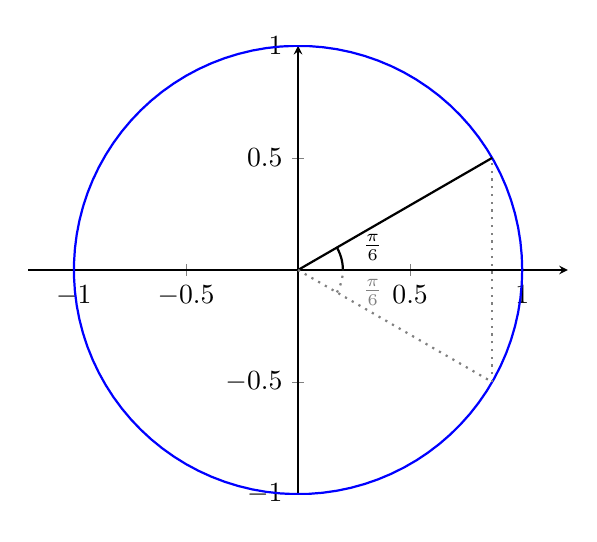
\begin{tikzpicture}
	\begin{axis}[xmin=-1,xmax=1,ymin=-1,ymax=1,axis x line=center,
	axis y line=center, axis equal]
	\addplot[blue,domain=0:2*pi,thick, samples=100] ({cos(deg(x))},{sin(deg(x))});
	\addplot[domain=0:sqrt(3)/2,thick] {1/sqrt(3)*x};
	\addplot[domain=0:pi/6,thick,samples=100] ({0.2*cos(deg(x))},{0.2*sin(deg(x))}) node[label={[label distance=2pt]0.5:\small$\frac{\pi}{6}$},pos=1] {};
	\addplot[domain=0:sqrt(3)/2,thick,gray,dotted] {-1/sqrt(3)*x};
	\addplot[domain=-pi/6:0,thick,samples=100,gray,dotted] ({0.2*cos(deg(x))},{0.2*sin(deg(x))}) node[label={[label distance=2pt]0.5:\small$\frac{\pi}{6}$},pos=0] {};
	\addplot[dotted,gray,thick] coordinates {(sqrt(3)/2, -1/2) (sqrt(3)/2, 1/2)};
	\end{axis}
	\end{tikzpicture}
	\caption{Opgave~\ref{it:trig3}}
	\label{fig:trig3}
\end{figure}

\item \label{it:trig4} I denne opgave beviser vi nogle af de eksakte værdier for sinus og cosinus til vinklen $ \frac{\pi}{4}$.
\begin{enumerate}
	\item Vis at $\sin(\frac{\pi}{4})=\frac{\sqrt{2}}{2}$ ved at regne på trekanten i Figur~\ref{fig:trig4}.(Hint: Pythagoras) 
	\item Brug idiotformlen til at vise at $\cos(\frac{\pi}{4})=\frac{\sqrt{2}}{2}$. 
\end{enumerate}

\begin{figure}
	\centering
	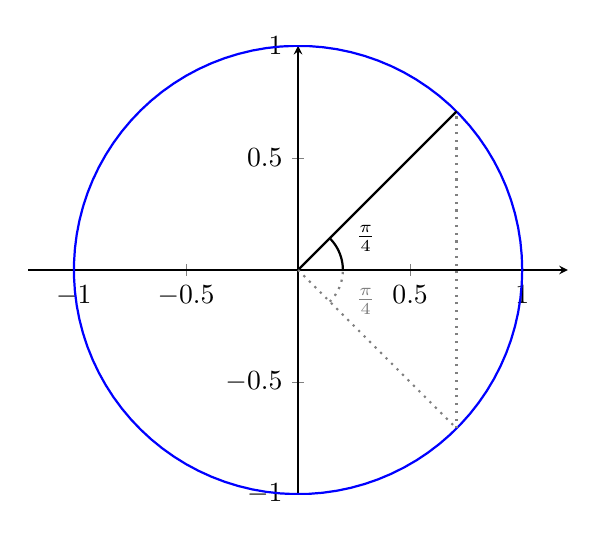
\begin{tikzpicture}
	\begin{axis}[xmin=-1,xmax=1,ymin=-1,ymax=1,axis x line=center,
	axis y line=center, axis equal]
	\addplot[blue,domain=0:2*pi,thick, samples=100] ({cos(deg(x))},{sin(deg(x))});
	\addplot[domain=0:sqrt(2)/2,thick] {1*x};
	\addplot[domain=0:pi/4,thick,samples=100] ({0.2*cos(deg(x))},{0.2*sin(deg(x))}) node[label={[label distance=2pt]0.5:\small$\frac{\pi}{4}$},pos=1] {};
	\addplot[domain=0:sqrt(2)/2,thick,gray,dotted] {-1*x};
	\addplot[domain=-pi/4:0,thick,samples=100,gray,dotted] ({0.2*cos(deg(x))},{0.2*sin(deg(x))}) node[label={[label distance=2pt]0.5:\small$\frac{\pi}{4}$},pos=0] {};
	\addplot[dotted,gray,thick] coordinates {({sqrt(2)/2}, -{sqrt(2)/2}) ({sqrt(2)/2}, {sqrt(2)/2})};
	\end{axis}
	\end{tikzpicture}
	\caption{Opgave~\ref{it:trig4}}
	\label{fig:trig4}
\end{figure}

\end{enumerate}

\section{Ligninger og uligheder}
\noindent En ligning består af to udtryk, en højre- og en venstreside, hvor mindst en af siderne indeholder en ubekendt variabel som vi gerne vil bestemme, samt et lighedstegn der binder de to sider sammen. Vores mål med ligninger er at bestemme alle de tal, som når vi sætter dem ind på den ubekendte variables plads gør at venstre siden er lig med højre siden. Dette kaldes også at løse ligningen.

\paragraph*{Eksempel:}
\begin{enumerate}
\item Løs ligningen $x + 2=7$:

Vi ser at $x=5$ er den eneste løsning til ligningen.
\item Løs ligningen $x=\sqrt{-2}$:

Vi husker fra tidligere kursusgange at dette er ensbetydende med at finde de $x$ der opfylder at $x^2=-2$, men da alle tal opløftet i anden giver noget positivt, har denne ligning ingen reelle løsning.
\item Løs ligningen $x^2 = 9$:

Vi ser at $x=3$ og $x=-3$ er de eneste løsninger til ligningen.

\item Løs ligningen $x+1 = \frac{1}{2}(2x+2)$:

Hvis vi reducere højresiden får vi
\begin{align*}
\frac{1}{2}(2x+2) = x+1,
\end{align*}
hvilket er sandt for alle $x$. Denne ligning har derfor uendeligt mange løsninger.
\end{enumerate}
Disse eksempler er alle meget ligetil og vi kan ved at betragte dem aflæse løsningerne. Det er dog ikke altid muligt og i disse tilfælde vil vi gerne kunne reducere vores ligning til en ny ligning med præcis samme løsningsmængde, men hvor vi nemt kan aflæse løsningerne. Sådanne ligninger kaldes ækvivalente ligninger og noteres med en biimplikationspil $\Leftrightarrow$.

\paragraph*{Regneregler:}
Når vi reducerer vores højre- og venstreside kan vi tænke på det som at de to er lig med hinanden. Det betyder at hvis vi gør noget på den ene side, så for at beholde ligheden er vi nødt til at gøre præcis det samme på den anden side.
\begin{enumerate}
\item Vi må lægge tal til og trække fra, så længe vi gør det samme på begge sider af lighedstegnet, f.eks.:
\begin{align*}
a + x = b \Leftrightarrow a+x \pm c = b \pm c, 
\end{align*}
hvor $a,b,c$ kan være alle tal.
\item Vi må gange begge sider med det samme tal, med undtagelse af $0$, f.eks.:
\begin{align*}
a + x = b \Leftrightarrow (a + x)c = bc \Leftrightarrow ac + xc = bc. 
\end{align*}
\item Vi må dividere begge sider med det samme tal, f.eks.:
\begin{align*}
a + x = b \Leftrightarrow \frac{a+x}{c} = \frac{b}{c} \Leftrightarrow \frac{a}{c}  + \frac{x}{c} = \frac{b}{c}.
\end{align*}
\end{enumerate}
Når vi løser ligninger vil vi gerne samle de ubekendte variable på den ene side, så vores reducerede ligning kommer til at ligne de nemme eksempler fra tidligere.

\paragraph*{Eksempler:}
\begin{enumerate}
\item Løs ligningen $4x+7 = 3(x+8)$:

Vi ganger først ind i parentesen på højresiden og derefter isolerer vi $x$ på venstresiden:
\begin{align*}
4x+7=3(x+8)= 3x+24 &\Leftrightarrow 4x+7-7 = 3x+24-7 \\
&\Leftrightarrow 4x = 3x + 17 \\
&\Leftrightarrow 4x - 3x = 3x + 17 - 3x \\
&\Leftrightarrow x = 17.
\end{align*}
\item Løs ligningen $\frac{2x+1}{4x}=3$:

Vi ganger først med nævneren på venstresiden for at få brøken væk og isolerer derefter $x$ på højresiden:
\begin{align*}
\frac{2x+1}{4x}=3 &\Leftrightarrow \frac{2x+1}{4x} \cdot 4x = 3 \cdot 4x \\
&\Leftrightarrow 2x+1 = 12x \\
&\Leftrightarrow 2x +1 - 2x = 12x - 2x \\
&\Leftrightarrow 1 = 10x\\
&\Leftrightarrow \frac{1}{10} = \frac{10x}{10} \\
&\Leftrightarrow \frac{1}{10} = x. 
\end{align*}
\item Løs ligningen $\pi x = 3-2x$:

Vi isolerer $x$ på venstresiden og trækker $x$ udenfor en parentes:
\begin{align*}
\pi x = 3-2x &\Leftrightarrow \pi x +2x = 3 - 2x + 2x \\
&\Leftrightarrow \pi x + 2x = 3 \\
&\Leftrightarrow x(\pi+2) = 3 \\
&\Leftrightarrow \frac{x(\pi + 2)}{\pi + 2} = \frac{3}{\pi +2} \\
&\Leftrightarrow x = \frac{3 }{\pi +2}.
\end{align*}
\end{enumerate}

\paragraph*{Nulreglen:}
Det er klart at hvis vi har to tal $a,b$ hvor ingen af dem er $0$, så giver $a \cdot b$ også noget der er forskelligt fra $0$. Det betyder at hvis vi har en ligning hvor to tal ganget sammen skal give $0$, så må det ene af de to tal være $0$. Det kan vi også skrive mere matematisk:
\begin{align*}
\textup{Hvis }a \cdot b = 0, \textup{ så er } a=0 \textup{ eller } b=0.
\end{align*}
Denne regel kaldes nulreglen og den er ekstremt nyttig når man skal løse ligninger hvor man kan trække den ubekendte variabel udenfor en parentes.

\paragraph*{Eksempler:}
\begin{enumerate}
\item Løs ligningen $2x^2+3x=0$:

Vi trækker $x$ udenfor en parentes:
\begin{align*}
2x^2+3x=0 &\Leftrightarrow x(2x+3)=0.
\end{align*}
Ved at bruge nulreglen ser vi nu at løsningerne er $x=0$ eller $2x+3=0 \Leftrightarrow x = \frac{-3}{2}$.
\end{enumerate}

\paragraph*{Uligheder}
Hvis vi erstatter lighedstegnet i en ligning med et ulighedstegn får vi en ulighed. Ligesom med ligninger vil vi gerne bestemme alle de tal vi kan sætte ind på den ubekendtes plads i vores ulighed, så den er sand. Det at løse en ulighed minder meget om at løse ligninger, men med den forskel at hvis vi ganger med et negativt tal på begge sider, så skal vi vende ulighedstegnet om. Det giver god mening da hvis vi f.eks. har uligheden $4 \leq 5$ og vi trækker først $5$ fra på begge sider og dernæst trækker $4$ fra på begge sider, så får vi
\begin{align*}
4 \leq 5 &\Leftrightarrow 4 - 5 \leq 5 - 5 \\
&\Leftrightarrow 4 - 5 - 4 \leq 5 - 5 - 4 \\
&\Leftrightarrow -5 \leq -4. 
\end{align*} 

\paragraph*{Regneregler:} 
Det giver os følgende regneregler til at løse uligheder:
\begin{enumerate}
\item Vi må lægge tal til og trække fra, så længe vi gør det samme på begge sider af ulighedstegnet, f.eks.:
\begin{align*}
a + x \leq b \Leftrightarrow a+x \pm c \leq b \pm c, 
\end{align*}
hvor $a,b,c$ kan være alle tal.
\item Vi må gange begge sider med det samme positive tal, f.eks.:
\begin{align*}
a + x \leq b \Leftrightarrow (a + x)c \leq bc \Leftrightarrow ac + xc \leq bc, 
\end{align*}
hvor $c$ er et positivt tal.
\item Vi må gange begge sider med det samme negative tal, hvis vi vender ulighedstegnet, f.eks.:
\begin{align*}
a + x \leq b \Leftrightarrow (a + x)d \geq bd \Leftrightarrow ad + xd \geq bd, 
\end{align*}
hvor $d$ er et negativt tal.
\item Vi må dividere begge sider med det samme positive tal, f.eks.:
\begin{align*}
a + x \leq b \Leftrightarrow \frac{a+x}{c} \leq \frac{b}{c} \Leftrightarrow \frac{a}{c}  + \frac{x}{c} \leq \frac{b}{c},
\end{align*}
hvor $c$ er et positivt tal.
\item Vi må dividere begge sider med det samme negative tal, hvis vi vender ulighedstegnet, f.eks.:
\begin{align*}
a + x \leq b \Leftrightarrow \frac{a+x}{d} \geq \frac{b}{d} \Leftrightarrow \frac{a}{c}  + \frac{x}{d} \geq \frac{b}{d},
\end{align*}
hvor $d$ er et negativt tal.
\end{enumerate}

\paragraph*{Eksempler:}
\begin{enumerate}
\item Løs uligheden $4+x \leq 5$:

Vi isolerer $x$ på venstresiden og får at $x \leq 1$.
\item Løs uligheden $-2x+4 \leq 3x$:

Vi isolerer $x$ på højresiden og får at $4 \leq 5x \Leftrightarrow \frac{4}{5} \leq x$.
\end{enumerate}



\section{Introduktion til differentialregning}
\begin{enumerate}
	\item Differentier funktionerne 
	\begin{align*}
	f_1(x)=2x+1,&& f_2(x)=x+\cos(x),&& f_3(x)=e^x-1,&&f_4(x)=\frac{1}{4}x^2+\ln(x).
	\end{align*}
	
	
	\item Bestem hældningen af funkionen $f(x)=x^3+x^2-x$ i punkterne $x=0$ og $x=1$.

	\item Brug regnereglen $\frac{d}{dx} x^n=nx^{n-1}$ til at differentiere funktionerne
	\begin{align*}
	f_1(x)=x^3,&& f_2(x)=\sqrt{x},&& f_3(x)=\frac{1}{x},&&f_4(x)=\frac{1}{x^2},&&f_5(x)=\frac{1}{\sqrt{x}}.
	\end{align*}
	\item \label{it:diff12} Bestem for hver af de blå grafer i Figur~\ref{fig:diff12} hvilken af de røde grafer der beskriver den afledede.
	
	\item Differentier funktionerne 
	\begin{align*}
	f(x)=3e^{2x}-\frac{1}{2}\ln x,&& g(x)=\frac{1}{2}\sin x,&& h(x)=\ln(\frac{x}{2})+3e^{-\frac{1}{6}x}.
	\end{align*}
	
	\item Differentier funktionerne
	\begin{align*}
	f(x)=x^7-2x^4-3x^2,&&g(x)=-x^5+4x^{\frac{3}{2}}-x^{-2},&&h(x)=\sqrt{x}+\frac{2}{x}.
	\end{align*}
	
	\begin{figure}
		\centering
		
		\begin{minipage}{0.3\linewidth}
			\begin{tikzpicture}[scale=0.5]
			\begin{axis}[xmin=-2,xmax=2,ymin=-2,ymax=2,axis x line=center,
			axis y line=center,ticks=none, restrict y to domain=-2:2]
			\addplot[thick,blue, samples = 600] {x^4-5/4*x^2+1/4};
			\end{axis}
			\end{tikzpicture}
		\end{minipage}
		\begin{minipage}{0.3\linewidth}
			\begin{tikzpicture}[scale=0.5]
			\begin{axis}[xmin=-2,xmax=2,ymin=-2,ymax=2,axis x line=center,
			axis y line=center,ticks=none]
			\addplot[thick,blue, samples = 200] {x+1/2};
			\end{axis}
			\end{tikzpicture}
		\end{minipage}
		\begin{minipage}{0.3\linewidth}
			\begin{tikzpicture}[scale=0.5]
			\begin{axis}[xmin=-2,xmax=2,ymin=-2,ymax=2,axis x line=center,
			axis y line=center,ticks=none, restrict y to domain=-2:2]
				\addplot[thick,blue, samples = 600] {x^3-x^2/2-x+1/2};
			\end{axis}
			\end{tikzpicture}
		\end{minipage}
%		
		\begin{minipage}{0.3\linewidth}
			\begin{tikzpicture}[scale=0.5]
			\begin{axis}[xmin=-2,xmax=2,ymin=-2,ymax=2,axis x line=center,
			axis y line=center,ticks=none]
				\addplot[thick,red, samples = 600] {3*x^2-x-1};
			\end{axis}
			\end{tikzpicture}
		\end{minipage}
		\begin{minipage}{0.3\linewidth}
			\begin{tikzpicture}[scale=0.5]
			\begin{axis}[xmin=-2,xmax=2,ymin=-2,ymax=2,axis x line=center,
			axis y line=center,ticks=none]
			\addplot[domain=-2:2,thick,red, samples = 600] {1};
			\end{axis}
			\end{tikzpicture}
		\end{minipage}
		\begin{minipage}{0.3\linewidth}
			\begin{tikzpicture}[scale=0.5]
			\begin{axis}[xmin=-2,xmax=2,ymin=-2,ymax=2,axis x line=center,
			axis y line=center,ticks=none, restrict y to domain=-2:2]
			\addplot[thick,red, samples = 200] {4*x^3-5/2*x};					
			\end{axis}
			\end{tikzpicture}
		\end{minipage}
		\caption{Opgave~\ref{it:diff12}}
		\label{fig:diff12}
	\end{figure}	
	
	
	\item Bestem, for hver af de følgende funktioner, de punkter hvor tangenthældningen er $2$.
	\begin{align*}
	f(x)=x^3+2x,&& f(x)=\frac{1}{3}x^3-3x^2+2x-1. 
	\end{align*}
	
	\item Differentier funktionerne 
	\begin{align*}
	f(x)=3\sqrt[3]{x},&& f(x)=(3x+4)x^2.
	\end{align*}
		

	\item Differentier funktionerne
	
	\begin{align*}
		f(x)=\frac{\sqrt{x}+1}{x},&& f(x)=\frac{x^2\sqrt{x^3}}{x^{-1/4}},&&f(x)=\ln\frac{1}{x^2}
	\end{align*}
	
	

	
	\item \label{it:diff11} Bestem for hver af de blå grafer i Figur~\ref{fig:diff11} hvilken af de røde grafer der beskriver den afledede.
		\begin{figure}
		\centering
		
		\begin{minipage}{0.3\linewidth}
			\begin{tikzpicture}[scale=0.5]
			\begin{axis}[xmin=-2,xmax=2,ymin=-2,ymax=2,axis x line=center,
				axis y line=center,ticks=none]
				\addplot[thick,blue, samples = 600] {e^(-x^2)};

				\end{axis}
			\end{tikzpicture}
		\end{minipage}
		\begin{minipage}{0.3\linewidth}
			\begin{tikzpicture}[scale=0.5]
			\begin{axis}[xmin=-2,xmax=2,ymin=-2,ymax=2,axis x line=center,
			axis y line=center,ticks=none,restrict y to domain=-2:2]
			\addplot[thick,blue, samples = 200] {1/(3*x)};
			\end{axis}
			\end{tikzpicture}
		\end{minipage}
			\begin{minipage}{0.3\linewidth}
		\begin{tikzpicture}[scale=0.5]
		\begin{axis}[xmin=-2,xmax=2,ymin=-2,ymax=2,axis x line=center,
		axis y line=center,ticks=none]
		\addplot[domain=-2:2,thick,blue, samples = 800] {x^4*cos(deg(x))};
		\end{axis}
		\end{tikzpicture}
	\end{minipage}

		\begin{minipage}{0.3\linewidth}
	\begin{tikzpicture}[scale=0.5]
	\begin{axis}[xmin=-2,xmax=2,ymin=-2,ymax=2,axis x line=center,
	axis y line=center,ticks=none,restrict y to domain=-2:2]
	\addplot[thick,red, samples = 200] {4*x^3*cos(deg(x))-x^4*sin(deg(x))};
	\end{axis}
	\end{tikzpicture}
\end{minipage}
\begin{minipage}{0.3\linewidth}
	\begin{tikzpicture}[scale=0.5]
	\begin{axis}[xmin=-2,xmax=2,ymin=-2,ymax=2,axis x line=center,
	axis y line=center,ticks=none,restrict y to domain=-2:2,restrict x to domain=-2:2]
	\addplot[,thick,red, samples = 200] {-2*x*e^(-x^2)};
	\end{axis}
	\end{tikzpicture}
\end{minipage}
\begin{minipage}{0.3\linewidth}
	\begin{tikzpicture}[scale=0.5]
	\begin{axis}[xmin=-2,xmax=2,ymin=-2,ymax=2,axis x line=center,
	axis y line=center,ticks=none,restrict y to domain=-2:2]
		\addplot[thick,red, samples = 600] {-1/(3*x^2)};
	\end{axis}
	\end{tikzpicture}
	\end{minipage}
	\caption{Opgave~\ref{it:diff11}}
	\label{fig:diff11}
	\end{figure}	
	

	
	\item Differentier funktionerne
	\begin{align*}
	f(x)=-\ln(\frac{1}{x^{-5}}),&& f(x)=\sqrt[3]{e^{9x}}.
	\end{align*}
	
	\end{enumerate}

\section{Andengradsligninger og to ligninger med to ubekendte}
Indtil videre har vi for det meste kun betragtet førstegradsligninger, som er ligninger på formen $ax+b=0$, hvor $a$ kan være et hvilket som helst tal med undtagelse af $0$ og $c$ kan være alle tal. Det næste vi skal undersøge er andengradsligninger, som er på formen $ax^2+bx+c=0$, hvor $a$ kan være alle tal bortset fra $0$, og $b,c$ kan være alle tal.

Vi finder løsningerne til en andengradsligning ud fra formlen
\begin{align*}
x = \frac{-b \pm \sqrt{b^2-4ac}}{2a} = \frac{-b \pm \sqrt{d}}{2a},
\end{align*}
hvor $a,b,c$ er de samme tal som indgår i den andengradsligning vi er ved at løse og $d=b^2-4ac$ kaldes diskriminanten. Løsningerne til en andengradsligning kaldes ofte for rødderne af andengradsligningen. 

Vi ser først på antallet af løsninger til en andengradsligning:
\begin{enumerate}
\item Hvis $d>0$ så har andengradsligningen præcis $2$ løsninger, givet ved
\begin{align*}
x_1 = \frac{-b+\sqrt{b^2-4ac}}{2a} \qquad \textup{ og } \qquad x_2=\frac{-b - \sqrt{b^2-4ac}}{2a}.
\end{align*}
\item Hvis $d=0$ så har andengradsligningen præcis $1$ løsning, givet ved
\begin{align*}
x = \frac{-b}{2a}.
\end{align*}
\item Hvis $d<0$ så har andengradsligningen ingen reelle løsninger (I modsætning til hvad mange får at vide i gymnasiet, så har den stadig løsninger, men dem vil I komme til at se i kurset \emph{Calculus}, og vi vil ikke komme mere ind på dem her).
\end{enumerate}

\paragraph*{Eksempler:}
\begin{enumerate}
\item Løs andengradsligningen $x^2+5x+4 = 0$:

Vi ser at $a=1$, $b=5$ og $c=4$. Dernæst udregner vi diskriminanten
\begin{align*}
d=b^2-4ac = 5^2-4\cdot 1 \cdot 4 = 25-16=9.
\end{align*}
Indsætter vi nu i løsningsformlen får vi
\begin{align*}
x=\frac{-b\pm\sqrt{d}}{2a} = \frac{-5\pm \sqrt{9}}{2 \cdot 1} = \frac{-5 \pm 3}{2} = \begin{cases} -1 \\
-4
\end{cases}.
\end{align*}
\item Løs andengradsligningen $x^2-3x+10=8$:

Før vi kan bruge løsningsformlen skal vi have højresiden til at være lig nul
\begin{align*}
x^2-3x+10=8 \Leftrightarrow x^2-3x +2 = 0.
\end{align*}
Vi ser at $a=1$, $b=-3$ og $c=2$, hvilket medfører at
\begin{align*}
d = b^2-4ac = (-3)^2 - 4 \cdot 1 \cdot 2 = 9-8 =1.
\end{align*}
Det giver os rødderne
\begin{align*}
x=\frac{-b \pm \sqrt{d}}{2a} = \frac{-(-3) \pm \sqrt{1}}{2 \cdot 1} = \frac{3 \pm 1}{2} =  \begin{cases} 2 \\
1
\end{cases}.
\end{align*}
\end{enumerate}


\paragraph*{Specialtilfælde:}
Hvis vi har nogle bestemte andengradspolynomier, så kan vi simplificere den generelle løsning.
\begin{enumerate}
\item Hvis $b=0$ så har vi andengradsligningen $ax^2+c=0$ det kan vi omskrive for at finde rødderne
\begin{align*}
ax^2+c=0 \Leftrightarrow x^2 = \frac{-c}{a} \Leftrightarrow x = \pm \sqrt{\frac{-c}{a}},
\end{align*}
givet at fortegnet på $a$ og $c$ er forskellige.
\item Hvis $c=0$ har vi andengradsligningen $ax^2+bx = 0$ og ved at sætte $x$ udenfor en parentes får vi
\begin{align*}
ax^2+bx = 0 \Leftrightarrow x(ax+b)=0.
\end{align*}
Nulreglen giver så at rødderne er
\begin{align*}
x_1=0 \qquad \textup{ og } \qquad x_2= \frac{-b}{a}.
\end{align*}
\end{enumerate}

\paragraph*{Faktorisering:}
Hvis vi har en andengradsligning $ax^2+bx+c=0$, så kan man omskrive venstresiden til
\begin{align*}
ax^2+bx+c = a(x-r_1)(x-r_2),
\end{align*}
hvor $r_1$ og $r_2$ er rødder til den givne andengradsligning. Dette kaldes at faktorisere sin andengradsligning. Det viser også at enhver andengradsligning er entydigt bestemt ud fra $a$ samt sine rødder, da vi, såfremt vi kender disse, kan genskabe den andengradsligning de kommer fra.

\paragraph*{Eksempel:}
\begin{enumerate}
\item Reducer udtrykket $\displaystyle \frac{2x^2+2x-4}{x-1}$.

Først finder vi rødderne for vores andengradspolynomium. Vi har at $d = b^2-4ac = 2^2-4\cdot 2 \cdot (-4) = 36$, hvilket medfører at vi har rødderne
\begin{align*}
x = \frac{-b\pm \sqrt{d}}{2a} = \frac{-2 \pm 6}{4} = \begin{cases} 1 \\ -2 \end{cases}.
\end{align*} 
Det betyder at vi kan faktorisere vores andengradspolynomium til
\begin{align*}
2x^2+2x-4 = 2(x-1)(x+2).
\end{align*}
Nu kan vi så reducere vores udtryk til
\begin{align*}
\frac{2x^2+2x-4}{x-1} = \frac{2(x-1)(x+2)}{x-1} = 2(x+2)=2x+4.
\end{align*}
\end{enumerate}
\paragraph*{To ligninger med to ubekendte:}
Indtil videre har vi kun betragtet én ligning med en ubekendt (ofte $x$) ad gangen. Det er ikke altid muligt at løse en ligning med flere ubekendte, men hvis vi har lige så mange ligninger som ubekendte så er det ofte muligt at løse dem. Vi vil her betragte to forskellige metoder til at løse sådanne ligningssystemer; \emph{substitutionsmetoden} og \emph{lige store koefficienters metode}. Vi vil primært holde os til to ligninger med to ubekendte men i kurset \emph{Lineær Algebra} vil i lære hvordan man effektivt kan løse flere ligninger med flere ubekendte.

Vi vil løse de følgende to ligninger med to ubekendte
\begin{align}
2x+y+3&=2y-4 \label{eq:1flereubekendte} \\
4x+2&=5y \label{eq:2flereubekendte}
\end{align}
først ved substitutionsmetoden og derefter ved brug lige store koefficienters metode.

I substitutionsmetoden starter vi med at isolere den ene af de ubekendte variable i en af ligningerne. Hvis vi starter med at isolere $x$ i \eqref{eq:1flereubekendte} får vi
\begin{align*}
2x+y+3 = 2y-4 &\Leftrightarrow 2x = y-7 \\
&\Leftrightarrow x = \frac{y-7}{2}.
\end{align*}
Det udtryk  kan vi så indsætte i \eqref{eq:2flereubekendte} så vi får én ligning med en ubekendt som vi kan løse
\begin{align*}
4x+2 = 5y &\Leftrightarrow 4 \cdot \frac{y-7}{2} + 2 = 5y \\
&\Leftrightarrow 2y-14 + 2 = 5y \\
&\Leftrightarrow -12 = 3y \\
&\Leftrightarrow y = -4.
\end{align*}
Indsætter vi nu dette udtryk for $y$ i \eqref{eq:2flereubekendte} får vi
\begin{align*}
4x+2=5 \cdot (-4) &\Leftrightarrow 4x+2=-20 \\
&\Leftrightarrow 4x = -22 \\
&\Leftrightarrow x = \frac{-22}{4} \\
&\Leftrightarrow x = \frac{-11}{2},
\end{align*}
hvilket betyder at løsningen til vores to ligninger med to ubekendte er $x= \frac{-11}{2}$ og $y=-4$. Bemærk at vi kunne også have indsat vores udtryk for $y$ i \eqref{eq:1flereubekendte}.


Idéen i lige store koefficienters metode er igen at omskrive de to ligninger til én ligning med en ubekendt, som vi godt kan løse og så derefter indsætte den variabel vi har fundet i en af de to givne ligninger, så vi igen har én ligning med én ubekendt bare med den anden ubekendte variabel.

Fra \eqref{eq:1flereubekendte} har vi, at $2x + y + 3 = 2y-4$, og ganger vi med $2$ på begge sider får vi at $4x+2y+6 = 4y-8$. Vi husker at vi gerne må trække noget fra på den ene side af en ligning, så længe vi trækker det samme fra på den anden side. Det betyder, at hvis vi trækker $4x + 2y +6$ fra på den ene side i \eqref{eq:2flereubekendte} så kan vi trække $4y-8$ fra på den anden side uden at ændre ved vores lighed. Det giver
\begin{align*}
4x+2-(4x+2y+6)= 5y-(4y-8) &\Leftrightarrow 4x+2-4x-2y-6= 5y-4y+8 \\
&\Leftrightarrow -4 -2y = y+8 \\
&\Leftrightarrow -12 = 3y \\
&\Leftrightarrow y=-4.
\end{align*}
Grunden til at vi gangede \eqref{eq:1flereubekendte} med $2$ før vi trak den fra \eqref{eq:2flereubekendte}, var for at få det samme til til at stå foran $x$ i begge ligninger. Det medførte at alle $x$'erne gik ud med hinanden i \eqref{eq:2flereubekendte}, og vi fik derfor én ligning med en ubekendt, som vi godt kunne løse. Vi mangler stadig at finde $x$, men det kan vi gøre ved at indsætte $y=-4$ i enten \eqref{eq:1flereubekendte} eller \eqref{eq:2flereubekendte} og så isolere $x$. Indsætter vi $y=-4$ i \eqref{eq:2flereubekendte} får vi
\begin{align*}
4x + 2 = 5 \cdot (-4) &\Leftrightarrow 4x+2 = -20 \\
&\Leftrightarrow 4x=-22 \\
&\Leftrightarrow x= \frac{-11}{2}.
\end{align*}
Det betyder at løsningen til vores to ligninger med to ubekendte er $x=\frac{-11}{2}$ og $y=-4$.
























%To typiske andengradspolynomier er afbilledet i Figur ~\ref{fig:andengradspolynomium1} og~\ref{fig:andengradspolynomium2}. De tre tal $a,b,c$ der indgår i et andengradspolynomium har direkte indflydelse på hvordan grafen for andengradspolymiet ser ud.
%
%\begin{figure}[!htbp]
%\begin{minipage}{0.49\textwidth}
%\centering
%  \pgfplotsset{width=0.5\textwidth,compat=1.11}
%  \centering
%  \begin{tikzpicture}
%  \begin{axis}[ 
%    xmin=-2.0,
%    xmax=2.0,
%    ymin=-2.0,
%    ymax=2.0,
%    axis equal,
%    %axis lines=middle,
% ticks=none,
%xlabel={},
%ylabel={},
%  ]
%\addplot[thick,blue,samples=300]{x^2+x-1}; 
%\node[below] at (2.2,0.0) {$x$}; 
%\node[left] at (0.0,1.8) {$y$}; 
%\end{axis}
% \end{tikzpicture}
%  \caption{$f(x)=x^2+x-1$}
%  \label{fig:andengradspolynomium1}
%\end{minipage}
%\begin{minipage}{0.49\textwidth}
%  \pgfplotsset{width=0.5\textwidth,compat=1.11}
%  \centering
%  \begin{tikzpicture}
%  \begin{axis}[ 
%    xmin=-2.0,
%    xmax=2.0,
%    ymin=-2.0,
%    ymax=2.0,
%    axis equal,
%    %axis lines=middle,
% ticks=none,
%xlabel={},
%ylabel={},
%  ]
%\addplot[thick,blue,samples=300]{-1*x^2+x+1}; 
%\node[below] at (2.2,0.0) {$x$}; 
%\node[left] at (0.0,1.8) {$y$}; 
%\end{axis}
% \end{tikzpicture}
%  \caption{$f(x)=-x^2 + x + 1$}
%  \label{fig:andengradspolynomium2}
%\end{minipage}
%\end{figure}
%

\newpage
\section{Math101 exercises}
\begin{enumerate}

	\item Differentiate the functions:
	\begin{align*}
	f_1(x)=\sqrt{x^2+1},&& f_2(x)=\frac{x}{2x+1},&& f_3(x)=x\sin(x).
	\end{align*}

	\item Differentiate the functions:
	\begin{align*}
	f_1(x)=xe^x,&& f_2(x)=2x^2\cos(x),&& f_3(x)=\ln(x)e^x,&& f_4(x)=\sin(x)\cos(x).
	\end{align*}

	\item Differentiate the functions:
	\begin{align*}
	f_1(x)=\frac{x}{x-1},&&f_2(x)=\frac{x^2-x+1}{3x+2},&&f_3(x)=\frac{x^2}{x^3-2x^2}.
	\end{align*}
	
	\item Differentiate the functions:
	\begin{align*}
	f_1(x)=(3x-1)^\frac{4}{3},&& f_2(x)=\ln(x^2+3x),&& f_3(x)=e^{2-x},&&f_4(x)=\sin(x^3).
	\end{align*}
	
	\item \label{it:diff24}Determine the derivative of $f(x)=(x-1)e^x$.
	
	
	\item \label{it:diff23}Determine the derivative of $f(x)=x\ln(x)-x$.
	
	\item Differentiate the functions:
	\begin{align*}
	f_1(x)=e^{x^3},&&f_2(x)=\cos^2(x),&&f_3(x)=\sin^3(x)&&f_4(x)=2\tan(x^2).
	\end{align*}
		
	\item\label{it:diff21} Show that 
	\begin{align*}
	\frac{d}{dx} \tan x= 1+\tan^2x.
	\end{align*}
	(Hint: Use that $\tan x=\frac{\sin x}{\cos x}$)

	\item Differentiate the function $f(x)=\frac{xe^x}{\cos(x)}$.
		
	\item Differentiate the function
	\begin{align*}
	f(x)=\cos^2(\sqrt{x^2+1}).
	\end{align*}
		
	\item Differentiate the functions:
	\begin{align*}
	f_1(x)=\frac{\cos^2(x)}{\sin(x)},&&f_2(x)=\frac{e^{x^2}}{x},&&f_3(x)= \frac{x\cos(x)}{e^x}
	\end{align*}
	
	\item Differentiate the functions:
	\begin{align*}
	f(x)=\frac{x^2e^x}{-x\ln(x)},&& g(x)=xe^x\ln x,&& h(x)=\tan(x)e^{x}\cos(x)x^2
	\end{align*}
	
	
\end{enumerate}

\chapter{Funktioner}
\section{Funktioner: Injektivitet, surjektivitet, summer og produkter}
Vi vil nu se nærmere på hvad en funktion egentlig er, for at gøre dette starter vi med at kigge kort på mængder. Lad $X$ og $Y$ være to mængder, det kan f.eks. være et interval som $[0,1]$ eller $(0,1)$, der henholdsvis består af alle tal der opfylder $0 \leq x \leq 1$ og $0 < x < 1$, eller en endelig mængde $\{a,b,c,d\}$. Hvis vi lader $X = \{1,2,3,4\}$ så siger vi f.eks. at $2$ ligger i $X$ og notere det med $2 \in X$ mens vi siger at $5$ ikke ligger i $X$ hvilket vi notere $5 \not\in X$. Hvis vi vil fjerne et element i en mængde skriver vi f.eks. $X \setminus 3 = \{1,2,4\}$. Derudover kan vi også tage en delmængde af en allerede givet mængde, hvilket vi notere f.eks. med $\{1,2\} \subset X$. For at simplificere vores notation vil vi ofte skrive intervallet $(-\infty,\infty)$ som $\mathbb{R}$ og kalde det for de reelle tal. 



Vi siger at $f$ er en funktion der går mellem $X$ og $Y$, skrevet $f \colon X \to Y$, hvis $f(x)$ giver præcis et element i $Y$ for alle $x \in X$. Vi kalder $X$ for domænet (også kaldet definitionsmængden) af $f$ og $Y$ for codomænet af $f$. Bemærk, at det betyder at hvis $f$ sender et element fra $X$ over i flere forskellige elementer i $Y$ så er $f$ ikke en funktion, men en funktion kan godt sende flere elementer fra $X$ over i det samme element i $Y$.

\paragraph*{Eksempler:}
\begin{enumerate}
\item Lad $f \colon \{1,2,3\} \to \{1,2,3,4,5,6\}$ være givet ved $f(x)=2x$, så er $f$ en funktion da ethvert element i $X$ bliver sendt over i præcis et element af $Y$. Bemærk, at vi behøver ikke ramme alle elementer i $Y$. 
\item Lad $f \colon \mathbb{R} \to \mathbb{R}$ være givet ved $f(x)=x^2$ så er $f$ en funktion.
\item Lad $X=\{a,b,c,d\}$ og $Y=\{1,2,\pi,\mathrm{abe}\}$ og bestem en funktion $f\colon X \to Y$. Det eneste der skal gælde for en funktion er, at den tager ethvert element i sit domæne og sender over i præcis et element i codomænet. Det  betyder at en mulig funktion $f$ er givet ved, $f(a)=1$, $f(b)=\pi$, $f(c)=\mathrm{abe}$  og $f(d)=2$. Dette kan også skrives som en ``gaffel funktion'' på følgende måde:
\begin{align*}
f (x) = \begin{cases} 
1 & x=a \\
\pi & x= b\\
\mathrm{abe} & x=c\\
2 & x=d
\end{cases}.
\end{align*}
Bemærk, at hvis vi f.eks. havde sat både $f(a)=1$ og $f(a)=2$ så havde $f$ ikke været en funktion!
\end{enumerate}

\paragraph*{Injektiv og surjektiv:}
Hvis $f \colon X \to Y$ er en funktion, så kalder vi alle de elementer i $Y$ som bliver ramt af $f$ for værdimængden af $f$. Bemærk, at vi på intet tidspunkt har sagt at vi skal ramme alle elementer i $Y$, derfor er værdimængden af $f$ en delmængde af codomænet for $f$. Vi siger derfor at en funktion $f$ er surjektiv hvis der gælder at værdimængden og codomænet for $f$ er den samme mængde, som det er tilfældet i Figur~\ref{fig:funktioner1etlec}.

Derudover har vi at hvis en funktion opfylder at der ikke er to forskellige elementer i $X$ der bliver sendt over i det samme element i $Y$, også skrevet
\begin{align*}
f(x_1) = y \textup{ og } f(x_2) =y \quad  \Rightarrow \quad x_1=x_2, 
\end{align*}
så siges funktionen at være injektiv, som f.eks. i Figur~\ref{fig:funktioner1tolec}. 

Hvis en funktion er både injektiv og surjektiv, så kalder vi den for en bijektiv funktion.

\begin{figure}[!htbp]
\begin{minipage}{0.49\textwidth}
  \pgfplotsset{width=0.5\textwidth,compat=1.11}
  \centering
  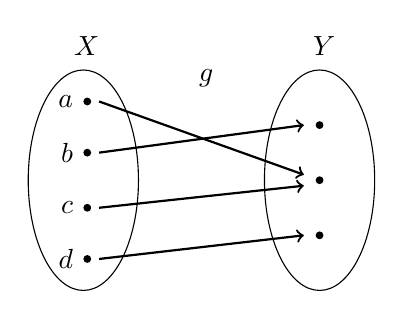
\begin{tikzpicture}
  \draw \boundellipse{0,0}{0.7}{1.4};
  \draw \boundellipse{3,0}{0.7}{1.4};
  \node[circle,fill,inner sep=1pt] at (0.05,1.0) [label=left:$a$]{};
  \node[circle,fill,inner sep=1pt] at (0.05,0.35) [label=left:$b$]{};
  \node[circle,fill,inner sep=1pt] at (0.05,-0.35) [label=left:$c$]{};
  \node[circle,fill,inner sep=1pt] at (0.05,-1.0) [label=left:$d$]{}; 
  \node[] at (0.45,1.7) [label=left:$X$]{}; 
  \node[circle,fill,inner sep=1pt] at (3.0,0.7) [label=right:]{};
  \node[circle,fill,inner sep=1pt] at (3.0,0.0) [label=right:]{};
  \node[circle,fill,inner sep=1pt] at (3.0,-0.7) [label=right:]{}; 
  \node[] at (3.45,1.7) [label=left:$Y$]{}; 
  \node[] at (1.9,1.3) [label=left:$g$]{}; 
  \draw[->,thick] (0.2,1.0) -- (2.8,0.07);
  \draw[->,thick] (0.2,0.35) -- (2.8,0.7);
  \draw[->,thick] (0.2,-0.35) -- (2.8,-0.07);
  \draw[->,thick] (0.2,-1.0) -- (2.8,-0.7);
 \end{tikzpicture}
  \caption{En surjektiv funktion}
  \label{fig:funktioner1etlec}
\end{minipage}
\begin{minipage}{0.49\textwidth}
\centering
  \pgfplotsset{width=0.5\textwidth,compat=1.11}
  \centering
  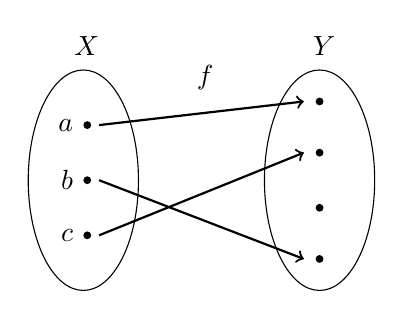
\begin{tikzpicture}
  \draw \boundellipse{0,0}{0.7}{1.4};
  \draw \boundellipse{3,0}{0.7}{1.4};
  \node[circle,fill,inner sep=1pt] at (0.05,0.7) [label=left:$a$]{};
  \node[circle,fill,inner sep=1pt] at (0.05,0.0) [label=left:$b$]{};
  \node[circle,fill,inner sep=1pt] at (0.05,-0.7) [label=left:$c$]{}; 
  \node[] at (0.45,1.7) [label=left:$X$]{}; 
  \node[circle,fill,inner sep=1pt] at (3.0,1.0) [label=right:]{};
  \node[circle,fill,inner sep=1pt] at (3.0,0.35) [label=right:]{};
  \node[circle,fill,inner sep=1pt] at (3.0,-0.35) [label=right:]{};
  \node[circle,fill,inner sep=1pt] at (3.0,-1.0) [label=right:]{}; 
  \node[] at (3.45,1.7) [label=left:$Y$]{}; 
  \node[] at (1.9,1.3) [label=left:$f$]{}; 
  \draw[->,thick] (0.2,0.7) -- (2.8,1);
  \draw[->,thick] (0.2,0.0) -- (2.8,-1.0);
  \draw[->,thick] (0.2,-0.7) -- (2.8,0.35);
 \end{tikzpicture}
  \caption{En injektiv funktion}
  \label{fig:funktioner1tolec}
\end{minipage}
\end{figure}

\paragraph*{Eksempler:}
\begin{enumerate}
\item Hvis $X=\{1,2,3,4\}$ og $Y= \{3,4,5,6,7\}$ så er funktionen $f \colon X \to Y$ givet ved $f(x)=x+2$ injektiv da ethvert $x \in X$ bliver sendt over i forskellige $y \in Y$ men den er ikke surjektiv, da $7$ ikke bliver ramt af noget $x \in X$.
\item Vi betragtede tidligere funktionen $f \colon \mathbb{R} \to \mathbb{R}$ givet ved $x^2$, denne funktion er hverken injektiv eller surjektiv da $-x$ og $+x$ bliver sent i det samme $y$, og vi rammer ikke hele $\mathbb{R}$ da $f(x)$ altid er positiv. Ved at ændre på domænet og codomænet kan vi gøre funktionen henholdsvis injektiv eller surjektiv. F.eks. er funktionen $f \colon [0,\infty) \to \mathbb{R}$ injektiv og $f \colon \mathbb{R} \to [0,\infty)$ er surjektiv. Vi ser endvidere at hvis vi har $f \colon [0,\infty) \to [0,\infty)$ så er $f$ endda bijektiv.
\end{enumerate}

\paragraph*{Sum og produkt af funktioner:}
Ligesom at vi kan lægge tal sammen og gange tal sammen, kan vi også gøre det samme med funktioner.

\paragraph*{Regneregler:}
Hvis $f$ og $g$ er funktioner, så har vi at
\begin{enumerate}
\item Summen af $f$ og $g$ evalueret i $x$ er det samme som at evaluere de to funktioner i $x$ og så lægge dem sammen:
\begin{align*}
(f\pm g)(x)=f(x) \pm g(x).
\end{align*}
\item Produktet af $f$ og $g$ evalueret i $x$ er det samme som at evaluere de to funktioner i $x$ og så gange dem sammen: 
\begin{align*}
(f \cdot g)(x)=f(x) \cdot g(x).
\end{align*}
\item At dividere funktionerne $f$ og $g$ og så evaluere i $x$ er det samme som at evaluere de to funktioner i $x$ og så dividere dem bagefter, såfremt $g(x)\neq 0$:
\begin{align*}
\Big(\frac{f}{g}\Big) (x) = \frac{f(x)}{g(x)},
\end{align*}
hvor $g(x) \neq 0$.
\end{enumerate}

\paragraph*{Eksempler:}
\begin{enumerate}
\item Hvis $f(x)=3x^2+1$ og $g(x)=\frac{1}{x}$ hvad er $(f+g)(2)$ så:

Vi udregner først $f(2)$ og $g(2)$:
\begin{align*}
f(2) &= 3 \cdot 2^2 + 1 = 3 \cdot 4 + 1 = 13, \\
g(2) &= \frac{1}{2},
\end{align*}
hvilket betyder at
\begin{align*}
(f+g)(2)=f(2)+g(2) = 13 + \frac{1}{2} = \frac{27}{2}.
\end{align*}
\item Hvis $f(x)=2x$ og $g(x)=\frac{1}{x}$ hvad er $\big(\frac{f}{g}\big)(3)$ så:

Vi udregner først $f(3)$ og $g(3)$:
\begin{align*}
f(3) &= 2 \cdot 3 = 6,\\
g(3) &= \frac{1}{3},
\end{align*}
hvilket medfører at 
\begin{align*}
\Big( \frac{f}{g}\Big) (3) = \frac{f(3)}{g(3)} = \frac{6}{\frac{1}{3}} = 6 \cdot 3 = 18.
\end{align*}
\end{enumerate}
\subsection{Opgaver}

\begin{enumerate}
	\item  Lad $A=\{1,2,3,4,5\}$ og $ B=\{ 3,5,\pi , 1,-1 \} $. Bestem en funktion $f\colon A\to B$ såedes at
	\begin{enumerate}
		\item $ f $ er injektiv og surjektiv.
%		\item $f $ er ikke injektiv men surjektiv.
%		\item $f$ er injektiv men ikke surjektiv.
		\item $f$ er hverken injektiv eller surjektiv.
	\end{enumerate}
	
	
	\item Kan cirklen med ligning $x^{2} +(y-1)^{2}=1$ beskrives som grafen af en funktion? Begrund dig svar, og i bekræftende tilfælde bedstem da funktionen.
	
	\item Givet mængderne 
	\begin{align*}
	A&= \{0,2,4,6,8\},\\
	B&=\{\text{Hund},\textup{Hest},\textup{Struds},\textup{Fugleedderkop},\textup{Laks},\textup{Mariehøne} \}
	\end{align*}
	bestem om følgende sammenhænge mellem $A$ og $B$ er funktioner. I bekræftende fald bestem også om de er injektive og/eller surjektive.
	\begin{enumerate}
		\item Lad $f\colon B\to A$ være givet ved
		\[f(x)=\textup{antal ben }x \textup{ har}.\]
		\item Lad $g$ være givet ved
		\begin{align*}
		g(0)&=\textup{Hund},\quad g(2)=\textup{Struds},\quad g(4)=\textup{Laks},\\ g(6)&=\textup{Fugleedderkop},\quad g(8)=\textup{Hest}
		\end{align*}
		
		\item Lad $ h\colon A\to B$ være givet ved at 
		\[h(x)= \textup{Dyerne i }B \textup{ som har } x \textup{ ben}.\] 
	\end{enumerate}

	\item Lad $f(x)=x^2-1$, $g(x)=\frac{1}{1+x}$. Bestem
	\begin{enumerate}
		\item $(f+g)(2)$
		\item $ \frac{f}{g}(-2) $
		\item $(fg)(0)$
		\item $\frac{g}{f}(x)$
		\item $(g-f)(x)$.
	\end{enumerate}

	\item Bestem værdimængden for funktionen $f\colon \mathbb{R}\to \mathbb{R}$ givet ved $f(x)=-3x^2+9$.
	
	\item \label{it:fun1} I Figur~\ref{fig:fun1} ses graferne for forskellige funktioner med definitionsmængde $[-2,2]$ og codomæne $[-2,2]$. Bestem for hver funktion om den er injektiv, surjektiv og/eller bijektiv.
	\begin{figure}
		\centering
	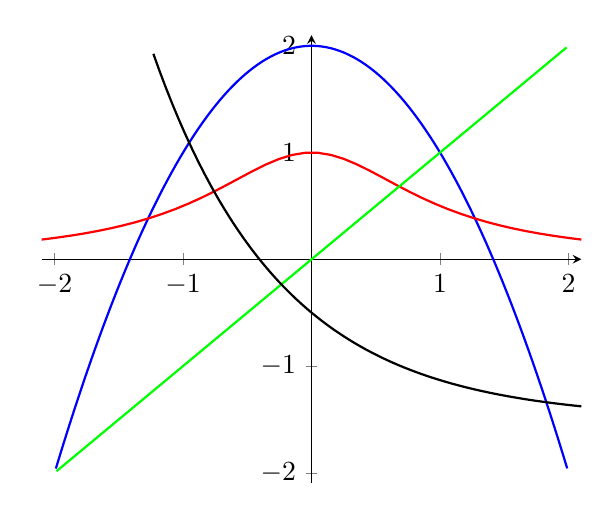
\begin{tikzpicture}
\begin{axis}[xmin=-2.1,xmax=2.1,ymin=-2.1,ymax=2.1,axis x line=center,
axis y line=center, restrict y to domain=-2:2]
\addplot[thick,blue,samples =300] {-x^2+2};
\addplot[thick,red,samples=100] {(1+x^2)^-1};
\addplot[thick,green, samples =200] {x };
\addplot[thick, black,samples=200] { e^-x -3/2};
\end{axis}
	\end{tikzpicture}
	\caption{Opgave~\ref{it:fun1}.}
	\label{fig:fun1}
	\end{figure}

	\item Bestem en mængde $D\subset \R$ således at funktionen $f\colon D\to \R$ givet ved $f(x)=x^2$ bliver injektiv.
	
	\item \label{it:fun2} På Figur~\ref{fig:fun2} ses grafen for funktionen $f(x)=x^{-1}$. Brug grafen til at afgøre om $f$ er injektiv, surjektiv og/eller bijektiv på $\R$. Hvis ikke $f$ er bijektiv bestem så det størst mulige domæne og codomæne således at $f$ bliver bijektiv.
	
	\begin{figure}
		\centering
		\begin{tikzpicture}
		\begin{axis}[xmin=-5,xmax=5,ymin=-20,ymax=20,axis x line=center,
		axis y line=center, restrict y to domain=-50:50]
		\addplot[thick,blue,samples=400] {1/x};
		\end{axis}
		\end{tikzpicture}
		\caption{Opgave~\ref{it:fun2}.}
		\label{fig:fun2}
	\end{figure}

	\item Brug \href{https://www.geogebra.org/m/eEE7RXzU}{Geogebra} til at bestemme for hvilke $a\in \{0,1,2,\dots,10\}$ funktionen $f\colon \R\to \R$ givet ved $f(x)=x^a$ er injektiv, surjektiv eller bijektiv. 
	
	\item Bestem den størst mulige definitionsmængde for funktionerne
	\begin{align*}
	f(x)=\sqrt{-x^2+x+2},&& g(x)=\frac{1}{(1+x^2)^\frac{1}{2}},&& h(x)=\frac{2}{\sqrt{x+2}}.
	\end{align*}
	
	\item \label{it:fun3exc} Figur~\ref{fig:fun3exc} viser forskellige kurver i planen. Argumenter for hvilke kurver der beskriver grafen for en funktion. 
	
 	\begin{figure}
		\centering
		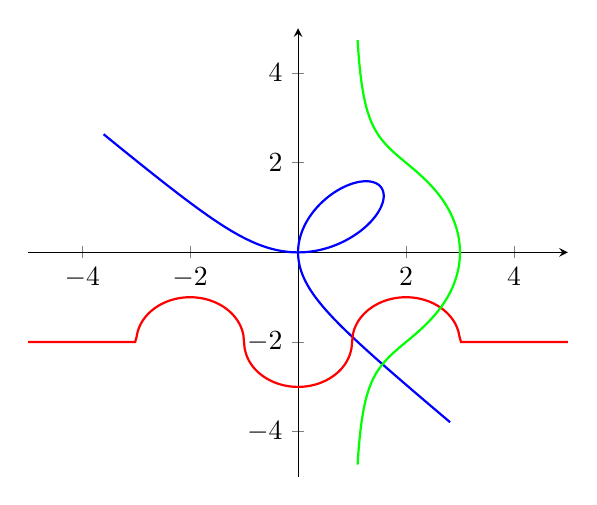
\begin{tikzpicture}[
		%declare function={func(\x)= (\x<-3)*(-2)+ and (\x>=-3,\x<=-1)*(sqrt(1-(x+2)^2)-2)+ and (\x>-1)*(-2); }
		declare function={
			func(\x)= (\x < -3) * (-2)   +
			and(x >= -3,\x<=-1) * (sqrt(1-(x+2)^2)-2)     +
			and(x >= -1,\x<=1) * (-sqrt(1-(x)^2)-2)     +
			and(x >= 1,\x<=3) * (sqrt(1-(x-2)^2)-2)     +
			(\x>3) * (-2)
			;
			}
		]
		\begin{axis}[xmin=-5,xmax=5,ymin=-5,ymax=5,axis x line=center,
	axis y line=center, restrict y to domain =-5:5]
		\addplot[data cs=polar, thick,blue,samples=200, domain= 0:180] ({x}, {3*sin(x)*cos(x)/(sin(x)^3+cos(x)^3)});
		\addplot[thick,red,samples=400] {func(x)};
		\addplot[data cs=polar, thick,green,samples=200, domain= 0:180] ({x}, {sec(x)+2*cos(x)});
		\end{axis}
		\end{tikzpicture}
		\caption{Opgave~\ref{it:fun3exc}.}
		\label{fig:fun3exc}
	\end{figure}

	\item Skitser grafen for en funktion som opfylder alle nedenstående puntker:
	\begin{enumerate}
		\item har domæne $[-2,4[$, og codomæne $[-2,4]$,
		\item går gennem punkterne $(-1,3)$ og $(2,-2)$,
		\item skærer y-aksen i $-2$,
		\item ikke skærer x-aksen.
		\end{enumerate}
	\item I \href{https://www.geogebra.org/m/eEE7RXzU}{Geogebra} er en kurve afbildet. Kurven afhænger af en parameter $a$. Bestem for hvilke (om nogen) $a\in \{-3,-2,\dots,2,3\}$ kurven beskriver grafen for en funktion.
\end{enumerate}

\section{Sammensatte og inverse funktioner}
Sidste gang beskæftigede vi os med funktioner $f \colon X \to Y$, hvor $X$ og $Y$ var mængder. Hvis vi har en anden funktion $g \colon Y \to Z$, hvor $Z$ også er en mængde, så kan man betragte sammensætningen af de to funktioner $g \circ f  \colon X \to Z$ (se Figur~\ref{fig:funktioner2et}) som er bestemt udfra formlen $(g \circ f)(x)=g(f(x))$ (bemærk at $g \circ f$ skal læses som at vi først anvender $f$ og dernæst $g$). Måden vi udregner $g \circ f$ er at indsætte funktionen $f$ på den ubekendte variabels plads  i $g$. I sådan et tilfælde kalder vi $f$ for den indre funktion, $g$ for den ydre funktion og $g \circ f$ for den sammensatte funktion.

\begin{figure}[!htbp]
  \pgfplotsset{width=0.5\textwidth,compat=1.11}
  \centering
  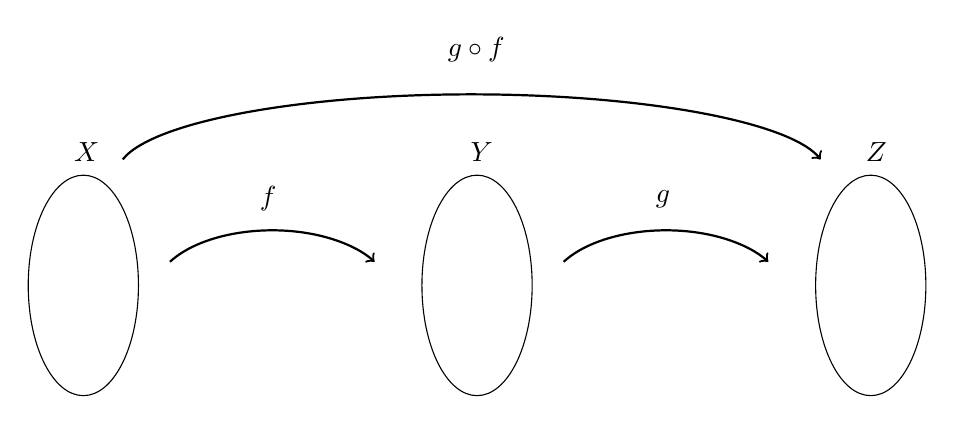
\begin{tikzpicture}
  \draw \boundellipse{0,0}{0.7}{1.4};
  \draw \boundellipse{5,0}{0.7}{1.4};
  \draw \boundellipse{10,0}{0.7}{1.4};
  \node[] at (0.45,1.7) [label=left:$X$]{};
  \node[] at (5.45,1.7) [label=left:$Y$]{}; 
  \node[] at (10.45,1.7) [label=left:$Z$]{}; 
  \node[] at (2.7,1.1) [label=left:$f$]{};
  \node[] at (7.7,1.1) [label=left:$g$]{};
  \node[] at (5.6,3.0) [label=left:$g \circ f$]{};
  \draw[thick,->] (0.5,1.6) arc (170:10:4.5 and 1.0);
  \draw[thick,->] (1.1,0.3) arc (150:30:1.5 and 0.8);
  \draw[thick,->] (6.1,0.3) arc (150:30:1.5 and 0.8);
 \end{tikzpicture}
  \caption{En sammensat funktion}
  \label{fig:funktioner2et}
\end{figure}

\paragraph*{Eksempler:}
\begin{enumerate}
\item Givet den sammensatte funktion $\frac{1}{x^2}$, find funktioner $f$ og $g$ så $f(g(x))=\frac{1}{x^2}$:

Vi genkender funktionerne $\frac{1}{x}$ og $x^2$ og ser at $x^2$ er sat ind på $x$ plads i $\frac{1}{x}$. Det betyder at hvis vi sætter $g(x)=x^2$ og $f(x)=\frac{1}{x}$ så har vi at $f(g(x))=\frac{1}{x^2}$.
\item Lad $f(x) = x^2+3x + \cos(x)$ og $g(x) = \tan(x)$ og bestem forskriften $(f \circ g)(x)$:

Vi indsætter $g(x)$ på $x$ plads i $f(x)$ og får:
\begin{align*}
(f \circ g)(x) = f(g(x))= (\tan (x))^2 + 3\tan(x) + \cos(\tan(x)).
\end{align*} 
\item Lad $f (x) = x^3$ og $g(x) = \sqrt{x}$ og bestem både $(g \circ f)(2)$ og $(f \circ g)(2)$:

Vi har at $f(2)=2^3 = 8$ og $g(2)=\sqrt{2}$, hvilket giver:
\begin{align*}
(g \circ f) (2) = g(f(2)) = g(8)=\sqrt{8}=\sqrt{4 \cdot 2} = \sqrt{4}\sqrt{2} = 2\sqrt{2}, \\
(f \circ g)(2) = f(g(2)) = f(\sqrt{2}) = (\sqrt{2})^3 = \sqrt{2^3} = \sqrt{8} = 2\sqrt{2}.
\end{align*}
\item Generelt kender vi funktioner så som 
\begin{align*}
\cos (x), \quad \sin (x),\quad \tan (x),\quad  x^2,\quad  \sqrt{x},\quad  \frac{1}{x}.
\end{align*} 
Hvis vi på $x$ plads i de forskellige funktioner indsætter en anden funktion, så vil vi få en sammensat funktion, som f.eks.
\begin{align*}
\cos(x^3), \quad  \sin (\sqrt{x}), \quad  \tan \Big( \frac{1}{x} \Big),\quad  (\sin(x))^2, \quad  \sqrt{\tan(x)}, \quad  \frac{1}{\cos(x)}.
\end{align*}
Bemærk, at der kan være forskel på at være den ydre og den indre funktion, f.eks. er $\sin (x^2)$ og $(\sin (x))^2$ ikke altid det samme.
\end{enumerate}
\paragraph*{Inverse funktioner:}
Hvis vi har to funktioner $f \colon X \to Y$ og $g \colon Y \to X$, som i Figur~\ref{fig:funktioner2to}, som opfylder at 
\begin{align*}
f(g(y))=y \qquad \textup{ og } \qquad g(f(x))=x,
\end{align*}
for alle $x \in X$ og $y \in Y$, så siges $f$ at være den inverse funktion til $g$ og ligelede siges $g$ at være den inverse funktion til $f$, hvilket også noteres med $g=f^{-1}$. Det betyder at den inverse funktion er en funktion der sender elementet $f(x)$ tilbage i det element det kom fra og tilsvarende for $g$. 

For at en sådan funktion kan eksistere skal $f$ være bijektiv, altså både injektiv og surjektiv. Hvis den ikke er injektiv så vil der være flere $x$'er der bliver sendt over i det samme $y$ men det betyder, at $f^{-1}(y)$ skal sende $y$ i mere end et punkt, hvilket ikke er muligt for en funktion. Derudover skal $f$ være surjektiv, da $f^{-1}$ skal kunne anvendes på alle elementer i $Y$ og det kan den ikke, medmindre $f$ rammer alle elementer i $Y$. 


\begin{figure}[!htbp]
  \pgfplotsset{width=0.5\textwidth,compat=1.11}
  \centering
  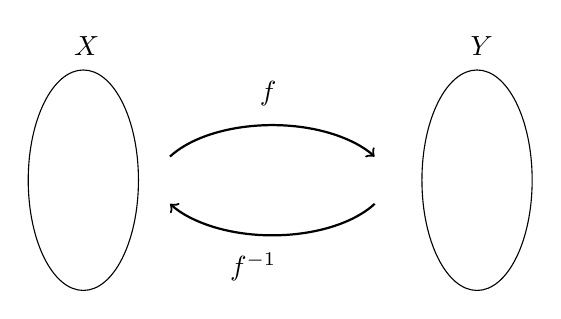
\begin{tikzpicture}
  \draw \boundellipse{0,0}{0.7}{1.4};
  \draw \boundellipse{5,0}{0.7}{1.4};
  \node[] at (0.45,1.7) [label=left:$X$]{};
  \node[] at (5.45,1.7) [label=left:$Y$]{}; 
  \node[] at (2.7,1.1) [label=left:$f$]{};
  \node[] at (2.7,-1.1) [label=left:$f^{-1}$]{};
  \draw[thick,->] (1.1,0.3) arc (150:30:1.5 and 0.8);
  \draw[thick,->] (3.7,-0.3) arc (330:210:1.5 and 0.8);
 \end{tikzpicture}
  \caption{En invers funktion}
  \label{fig:funktioner2to}
\end{figure}

\paragraph*{Eksempler:}
\begin{enumerate}
\item Lad $f \colon [0,\infty) \to [0,\infty)$ og $g(x) \colon [0,\infty) \to [0,\infty)$ være givet ved henholdsvis $f(x)=x^2$ og $g(x)=\sqrt{x}$, så har vi at
\begin{align*}
f(g(x))=(\sqrt{x})^2=x \qquad \textup{ og } \qquad g(f(x)) = \sqrt{x^2} = x,
\end{align*}
så $g=f^{-1}$. Bemærk, at vi ikke kan udvide $f$ og $g$ til hele $\mathbb{R}$, da de så ikke er bijektive.
\item Lad $f \colon \mathbb{R} \to \mathbb{R}$ og $g \colon \mathbb{R} \to \mathbb{R}$ være givet ved henholdsvis $f(x)=3x+2$ og $g(x)=\frac{1}{3}x-\frac{2}{3}$, så har vi at
\begin{align*}
f(g(x))= 3\Big(\frac{1}{3}x - \frac{2}{3}\Big) + 2 = x - 2 + 2 = x \\
g(f(x)) = \frac{1}{3}(3x+2) - \frac{2}{3} = x + \frac{2}{3} - \frac{2}{3} = x ,
\end{align*}
hvilket betyder at $g=f^{-1}$.
\end{enumerate}
\subsection{Opgaver}

\begin{enumerate}
	
	\item Det oplyses at $f(1)=2$, $f(4)=1$, $g(1)=1$ og $g(2)=4$ for to funktioner $f$ og $g$. Bestem
	\begin{enumerate}
		\item $f(g(2))$
		\item $g(f(1))$
		\item $g(f(f(4)))$
	\end{enumerate}
	
	\item Lad $f,g$ være givet ved $f(x)=x^2$ og $g(x)=1/(1+x)$ på domænet $(0,\infty)$. Er $f\circ g=g\circ f$? 
	
	\item \label{it:ssfunk1} Lad $f(x)=x^2$ og $g(x)=\cos(x)$. På Figur~\ref{fig:ssfunk1} er graferne for $f\circ g$ of $g\circ f$ plottet. Bestem for hver graf den tilhørende funktionsforskrift.
	
	\begin{figure}
		\centering
		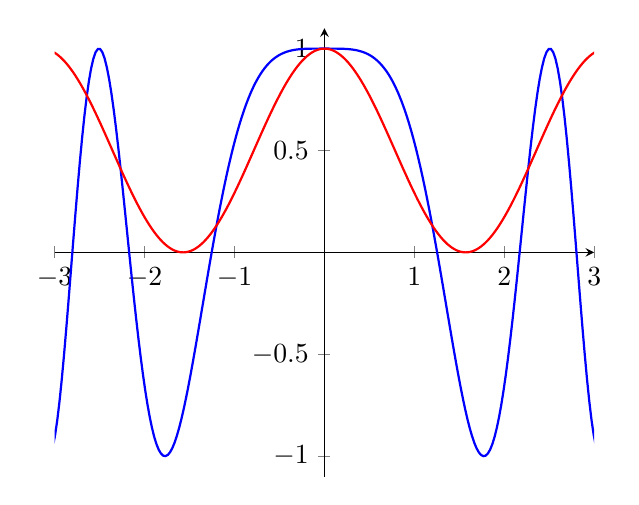
\begin{tikzpicture}
		\begin{axis}[xmin=-3,xmax=3,ymin=-1.1,ymax=1.1,axis x line=center,
		axis y line=center, restrict y to domain =-5:5]
		\addplot[thick,blue,samples=400] {cos(deg(x^2))};
		\addplot[thick,red,samples=400] {(cos(deg(x)))^2};
		\end{axis}
		\end{tikzpicture}
		\caption{Opgave~\ref{it:ssfunk1}}
		\label{fig:ssfunk1}
	\end{figure}
	
	\item Bestem $f\circ g$ og $g\circ f$ hvor $f(x)=\frac{1}{2}$ og $g(x)=4x^2+2x-1$.
	
	\item Lad $f\colon \{1,2,3\}\to \{a,b,c\}$ være givet ved $f(1)=b$, $ f(2)=a $, $ f(3)=c $. Bestem $g\colon \{a,b,c\}\to \{1,2,3\}$ så $g=f^{-1}$.
	
	\item Lad $f,g,h$ være funktioner defineret på $(0,\infty)$ givet ved
	\begin{align*}
	f(x)&=\sqrt{x},\\
	g(x)&=\frac{1}{1+x},\\
	h(x)&=\Big(\frac{1}{x}-1 \Big)^{2}.
	\end{align*}
	Bestem forskriften for følgende funktioner:
	\begin{enumerate}
		\item $f\circ g$,
		\item $g\circ f$,
		\item $f\circ h\circ g$,
		\item $g\circ h \circ f$,
		\item $ f\circ g \circ h $,
		\item $g\circ g$.
	\end{enumerate}
	
	
	\item Bestem den inverse funktion til $f\colon \R\setminus \{0\}\to \R\setminus\{0\}$ givet ved $f(x)=x^{-1}$. (Hint: Hvad er $f(f(x))$.)
	
	\item Vis at funktionerne $f\colon \R\setminus \{ \frac{1}{2}\}\to \R\setminus \{-\frac{1}{2} \}$ og $g\colon \R\setminus \{- \frac{1}{2}\} \to \R\setminus \{\frac{1}{2}\}$ givet ved
	\begin{align*}
	f(x)=\frac{x-1}{1-2x},&&g(x)=\frac{x+1}{1+2x},
	\end{align*}
	er inverse funktioner.
	
	\item Lad $f(x)=\cos((x-2)^2)$
	\begin{enumerate}
		\item Bestem funktioner $g$, $h$ så $f(x)=g(h(x))$.
		\item Bestem to andre funktioner $g_1$, $h_1$ så $f(x)=g_1(h_1(x))$
		\item Bestem tre funktioner $f_1,f_2,f_3$ så $f(x)=f_1(f_2(f_3(x)))$
	\end{enumerate}
	
	
	\item Lad funktionen $f(x)=e^{x^2}$ og bestem funktioner $g$ og $h$ så $f=g\circ h$.
	
	\item Lad $f\colon \R\to [-2,\infty[$ være givet ved $f(x)=(x-\sqrt{2})(x+\sqrt{2})$ og lad $g\colon [-2,\infty[\to [0,\infty[$ være givet ved $g(x)=\sqrt{x+2}$.
	\begin{enumerate}
		\item Bestem definitionsmængde, værdimængde og funktionsforskrift for $f\circ g$
		\item Er $g$ og $f$ inverse funktioner? (Hint: hvad er $(g\circ f)(-1)$?)
		\item Bestem en passende definitionsmængde $D$ så $f\colon D\to [-2,\infty[$ er invers til $g$.
	\end{enumerate}
	
		
	
	\item Betragt funktionerne $f\colon [0,\infty)\to [0,\infty)$ og $g\colon [0,\infty)\to[1,\infty)$ givet ved $f(x)=x^{3/2}$ og $g(x)=x^{2/3}+1$. 
	\begin{enumerate}
		\item Bestem det størst mulige domæne $D$ for funktionen $h\colon D\to \R$ givet ved $h(x)=x-1$ så sammensætningen $f \circ h$ er defineret.
		\item Vis at $g^{-1}=f\circ h$.
		\end{enumerate}
	
	%	
	
	
	
\end{enumerate}

\section{Polynomier}
Vi betragtede tidligere første- og andengradsligninger, hvor venstre siden var på formen $ax+b$ og $ax^2+bx+c$, henholdsvis. Dette er to eksempler på funktionstyper som man kalder polynomier. Disse funktioner vil vi nu studere mere dybdegående. 

\paragraph*{Førstegradspolynomier:}
En funktion med forskrift
\begin{align*}
f(x)=ax+b,
\end{align*}
hvor $a \in \mathbb{R}\setminus \{0\}$ og $b \in \mathbb{R}$, kaldes for et førstegradspolynomium. I genkender formentlig et førstegradspolynomium som ligningen for en ret linje.
\begin{figure}[!htbp]
  \centering
  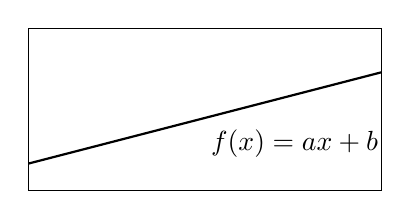
\begin{tikzpicture}
  \begin{axis}[ 
  	width=0.5\textwidth,
  	height=0.3\textwidth,
    xmin=-0.1,
    xmax=3,
    ymin=-0.1,
    ymax=1,
    %axis equal,
    %axis lines=center,
	ticks=none,
	restrict y to domain =0:1]
	\addplot[thick] {0.2*x+0.1} node[below right,pos=0.4] {$f(x)=ax+b$};
\end{axis}
 \end{tikzpicture}
  \caption{Førstegradspolynomium.}
  \label{fig:funktioner3et}
\end{figure}

Hvis vi sætter $x=0$ i vores førstegradspolynomium får vi at 
\begin{align*}
f(0)=a\cdot 0 + b = b,
\end{align*}
hvilket viser at et førstegradspolynomium skærer $y$-aksen i $b$. Derudover får vi, hvis vi indsætter $x+1$ på $x$ plads at
\begin{align*}
f(x+1)=a(x+1)+b = a + (ax+b)=a+f(x),
\end{align*}
hvilket viser at hvis vi går $1$ ud ad $x$-aksen, så gå vi $a$ op ad $y$-aksen og vi kalder derfor $a$ for hældningen af vores rette linje.

Hvis man får givet to punkter $(x_1,y_1)$ og $(x_2,y_2)$ i et koordinatsystem, så kan man bestemme forskriften for den rette linje der går gennem de to punkter ud fra formlerne
\begin{align*}
a= \frac{y_2-y_1}{x_2-x_1} \qquad \textup{ og } \qquad b= f(x_1)-ax_1 = y_1 - ax_1.
\end{align*}
Bemærk, at man også kan bruge punktet $(x_2,y_2)$ til at finde $b$.

\paragraph*{Eksempler:}
\begin{enumerate}
\item Givet punkterne $P=(1,7)$ og $Q=(2,4)$, bestem en forskrift for $f$:

Vi udregner først $a$:
\begin{align*}
a= \frac{y_2-y_1}{x_2-x_1} = \frac{4-7}{2-1}=\frac{-3}{1}=-3.
\end{align*}
Det bruger vi så sammen med punktet $P$ til at bestemme $b$:
\begin{align*}
b=y_1 - ax_1=7- (-3) \cdot 1 = 10, 
\end{align*}
hvilket giver at forskriften for $f$ er givet ved $f(x)=-3x+10$.
\item Lad funktionerne $f$ og $g$ være givet ved henholdsvis $f(x)=-x+2$ og $g(x)=2x+2$ og find det punkt hvor de skærer hinanden.

Vi vil finde den værdi for $x$ der gør at $f(x)=g(x)$. Det gør vi ved at sætte de to forskrifter lig med hinanden og så isolere $x$:
\begin{align*}
f(x)=g(x) &\Leftrightarrow -x+2 = 2x+2 \\
&\Leftrightarrow -3x = 0 \\
&\Leftrightarrow x = 0.
\end{align*}
Ved at indsætte $x=0$ i forskriften for enten $f$ eller $g$ får vi at $y=2$, hvilket viser at $f$ og $g$ skærer hinanden i punktet $(0,2)$.
\end{enumerate}

\paragraph*{Andengradspolynomier:}
En funktion med forskrift
\begin{align*}
f(x)=ax^2+bx+c,
\end{align*}
hvor $a \in \mathbb{R} \setminus \{0\}$ og $b,c \in \mathbb{R}$, kaldes for et andengradspolynomium. Grafen for et andengradspolynomium er en parabel (se Figur~\ref{fig:funktioner3to}).
\begin{figure}[!htbp]
  \centering
  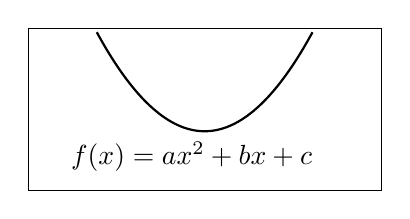
\begin{tikzpicture}
  \begin{axis}[ 
  	width=0.5\textwidth,
  	height=0.3\textwidth,
    xmin=-3,
    xmax=3,
    ymin=-0.1,
    ymax=1,
%    axis equal,
%    axis lines=center,
	ticks=none,
	restrict y to domain =0:1]
	\addplot[thick,samples=200] {0.2*x^2+0.2+0.1} node[below,pos=0.5] {$f(x)=ax^2+bx+c \phantom{ss}$};
\end{axis}
 \end{tikzpicture}
  \caption{Andengradspolynomium.}
  \label{fig:funktioner3to}
\end{figure}

Ved at sætte $x=0$ får vi, at et andengradspolynomium skærer $y$-aksen i
\begin{align*}
f(0)=a\cdot 0^2 + b \cdot 0 + c = c.
\end{align*}
Hvis vi differentierer $f(x)$, får vi
\begin{align*}
f'(x)=2ax+b,
\end{align*}
og ved igen at indsætte $x=0$ får vi at $f'(0)=b$. Vi husker at den afledte funktion beskriver hældningen i punktet, hvilket medfører, at $b$ beskriver hvad hældningen af vores andengradspolynomium er i skæringspunktet med $y$-aksen.

Til sidst ser vi, at hvis $x$ bliver meget stor, så bliver $x^2$ meget større end $x$ gør. Det betyder, at leddet $ax^2$ bestemmer om $f(x)$ går mod $+ \infty$ eller $-\infty$ når $x$ bliver meget stor. Da $x^2$ altid er positiv, har vi, at fortegnet på $a$ bestemmer om vores parabel går opad eller nedad. 

Hvis man får givet tre punkter $(x_1,y_1)$, $(x_2,y_2)$ og $(x_3,y_3)$, kan man entydigt bestemme det andengradspolynomium der går gennem de punkter ved at løse de tre ligninger med tre ubekendte:
\begin{align*}
f(x_1)&=ax_1^2+bx_1+c = y_1, \\
f(x_2)&=ax_2^2+bx_2+c = y_2, \\
f(x_3)&=ax_3^2+bx_2+c = y_3.
\end{align*}

\paragraph*{Toppunktsformlen:}
Hvis $a > 0$ i vores andengradspolynomium så kaldes det punkt med den mindste funktionsværdi for andengradspolynomiets toppunkt og hvis $a < 0$ så kaldes punktet med den største funktionsværdi for toppunktet. Vi notere toppunktet med $(x_0,y_0)$, hvor $x_0$ og $y_0$ kan bestemmes ud fra formlerne
\begin{align*}
x_0 = \frac{-b}{2a} \qquad \textup{ og } \qquad y_0=\frac{-d}{4a},
\end{align*}
hvor vi husker at $d=b^2-4ac$.


\paragraph*{Eksempler:}
\begin{enumerate}
\item Lad $f(x)= 2x^2+2x-2$ og bestem funktionens toppunkt.

Vi ser at $a=2$, $b=2$ og $c=-2$, hvilket medfører at $d=2^2-4 \cdot 2 \cdot (-2)=20$. Indsætter vi dette i formlerne for toppunktet får vi
\begin{align*}
x_0 = \frac{-2}{4} = \frac{-1}{2} \qquad \textup{ og } \qquad y_0 = \frac{-20}{8}=\frac{-5}{2},
\end{align*}
hvilket giver at toppunktet er $\big(\frac{-1}{2},\frac{-5}{2}\big)$.
\item Givet de tre punkter $(-1,1)$, $(0,1)$ og $(-2,-2)$, bestem en ligning for det dertilhørende andengradspolynomium.

Vi har de tre ligninger
\begin{align*}
a(-1)^2+b(-1) + c = 1 &\Leftrightarrow a-b+c=1,\\
a(0)^2+b(0) + c = 1 &\Leftrightarrow c=1,\\
a(-2)^2+b(-2) + c = -2 &\Leftrightarrow 4a-2b +c = -2.
\end{align*}
Fra ligning to ser vi at $c=1$ og ved at indsætte dette i de to andre, får vi to ligninger med to ubekendte:
\begin{align*}
a-b+1=1 &\Leftrightarrow a-b=0, \\
4a-2b+1=-2 &\Leftrightarrow 4a-2b = -3.
\end{align*}
Hvis vi benytter de lige store koefficienters metode til at løse disse to ligninger, får vi at
\begin{align*}
4a-2b = -3 &\Leftrightarrow 4a - 2b -4(a-b) = -3 \\
&\Leftrightarrow 2b = -3 \\
&\Leftrightarrow b = \frac{-3}{2}.
\end{align*}
Indsætter vi nu dette i ligningen $a-b=0$ får vi at $a=\frac{-3}{2}$, så vores andengradspolynomium er:
\begin{align*}
f(x)=-\frac{3}{2}x^2 -\frac{3}{2}x+1.
\end{align*}
\end{enumerate}













\subsection{Opgaver}

\begin{enumerate}
	\item Lad $f(x)=12x-3$, $ g(x)=-x^2-3x+1$ og bestem 
	\begin{align*}
	f\Big(-\frac{1}{3}\Big),&&f(-1),&& (f+g)(-2).
	\end{align*} 
	Bestem også $x$ så $f(x)=0$.
	
	\item \label{it:poly1} På Figur~\ref{fig:poly1} ses graferne for funktionerne
	\begin{align*}
		f(x)=x-2,&& g(x)=-\frac{1}{2}x+1,&&h(x)=5x+9.
	\end{align*}
	Bestem hvilke grafer hører til hvilke funktioner.
	\begin{figure}
		\centering
		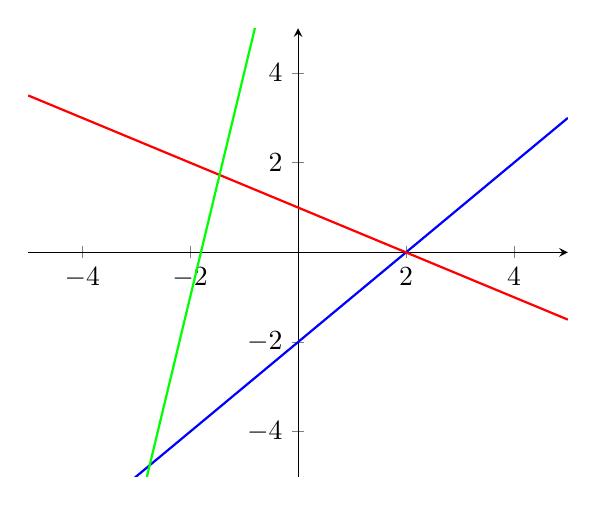
\begin{tikzpicture}
		\begin{axis}[xmin=-5,xmax=5,ymin=-5,ymax=5,axis x line=center,
		axis y line=center]
			\addplot[thick,blue] {x-2};
			\addplot[thick,red] {-x/2+1};
			\addplot[thick,green] {5*x+9};
		\end{axis}
		\end{tikzpicture}
		\caption{Opgave~\ref{it:poly1}}
		\label{fig:poly1}
	\end{figure}
	
	\item Bestem toppunktet for polynomiet $-2x^2+3x-1$
	
	\item Bestem hjørnepunkterne i den trekant som ses i Figur~\ref{fig:poly1}.
	
	\item Grafen for funktionen $f(x)=ax+b$ går gennem punkterne $(-1,3)$ og $(2,-1)$. Bestem $a$ og $b$.
	
	\item Lad $f(x)=2x-3$ og bestem $x_0$ så $ f(x_0)=x_0 $.
	
	\item Lad $ f(x)=\frac{3}{4}x^2-7x+5 $ og bestem først $f(-2)$ og derefter alle $x_0$ så $ f(x_0)=x_0 $
	
	\item Bestem koefficienterne $b$ og $c$ således at $f(x)=-x^2+bx+c$ har rødder $-2$ og $3$.
	
	\item Bestem et andengradspolynomium som går gennem punkterne $(-1,2)$, $(1,-1)$, $(2,4)$
	
	\item Bestem skæringspunkterne mellem $f(x)=2x^3-x^2+x-1$ og $h(x)=2x-1$.
	
	\item \label{it:poly2} På Figur~\ref{fig:poly2} ses grafen for et andengradspolynomium $f(x)=ax^2+bx+c$. Bestem fortegnene for $a,b,c,d$ ud fra grafen ($d$ betegner diskriminanten).
	
	\begin{figure}
		\centering
		\begin{tikzpicture}
		\begin{axis}[xmin=-1,xmax=2,ymin=-2,ymax=3,axis x line=center,
		axis y line=center,ticks=none]
			\addplot[thick,blue,samples=200]{2*x^2-2*x-1};
		\end{axis}
		\end{tikzpicture}
		\caption{Opgave~\ref{it:poly2}}
		\label{fig:poly2}
	\end{figure}
	
	\item \label{it:poly3} Figur~\ref{fig:poly3} viser skæringerne mellem $f(x)=2x^3-x^2-3x+2$ og $g(x)=-x^2-x+2$. Bestem skæringspunkterne mellem disse to polynomier.
	\begin{figure}
		\centering
		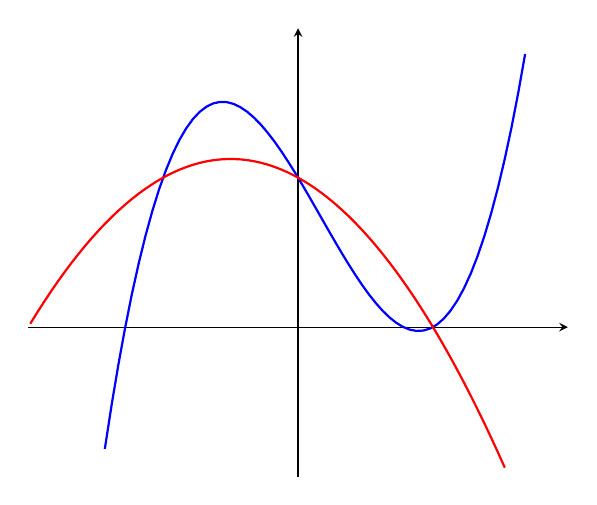
\begin{tikzpicture}
		\begin{axis}[xmin=-2,xmax=2,ymin=-2,ymax=4,axis x line=center,
		axis y line=center,ticks=none,restrict y to domain=-2:4,restrict x to domain=-2:2]
		\addplot[blue,thick,samples=200] {2*x^3-x^2-3*x+2};
		\addplot[red,thick,samples=200] {-x^2-x+2};]
		\end{axis}
		\end{tikzpicture}
		\caption{Opgave~\ref{it:poly3}}
		\label{fig:poly3}
	\end{figure}
	

	
	\item Lad $f(x)=2x^2-bx+1$ (se \href{https://www.geogebra.org/m/B5GvWyYW}{Geogebra}) og bestem
	\begin{enumerate}
		\item For hvilke værdier af $b$ ligger toppunktet for $f$ i første kvadrant?
		\item For hvilke værdier af $b$ ligger toppunktet for $f$ i tredje kvadrant?
	\end{enumerate}
	
	\item Lad $a_0$ og $c_0$ være faste tal og lad $f(x)=a_0 x^2+bx+c_0$ være et polynomium hvor $b$ er vilkårlig. Vis, at toppunktet for $f$ ligger på parablen $-a_0 x^2+c_0$ uanset værdien af $b$. Se eventuelt \href{https://www.geogebra.org/m/B5GvWyYW}{Geogebra}
\end{enumerate}

\section{Logaritme-og eksponentialfunktioner}
Vi definerer logaritmen $\log_a \colon (0,\infty) \to \mathbb{R}$ ved
\begin{align*}
\log_a(x) = y \quad \textup{ hvis og kun hvis } \quad a^y=x,
\end{align*}
hvor $a>0$ kaldes for grundtallet af logaritmefunktionen. Det skal forstås således at $\log_a(x)$ giver det tal, som $a$ skal opløftes i for at give $x$. Hvis grundtallet $a=e$, hvor $e$ er Eulers tal, så skriver vi $\ln(x)$ i stedet for $\log_e(x)$ og kalder det for den naturlige logaritme. Bemærk, at ud fra den måde vi definerede $\log_a(x)$ har vi, at
\begin{align}\label{eq:funktioner4et}
\log_a(a^y)=y \qquad \textup{ og } \qquad a^{\log_a(x)}=x.
\end{align}

\paragraph*{Eksempler:}
\begin{enumerate}
\item Udregn $\log_2(8)$:

For at udregne $\log_2(8)$ skal vi finde et $y$ som opfylder at $2^y=8$, hvilket vi ser er $y=3$. Derfor har vi at $\log_2(8)=3$.
\item Udregn $\log_{10}(10000)$:

Vi ser at $10000=10^4$ hvilket medfører at $\log_{10}(10000)=4$.
\item Udregn $\log_a(1)$:

Vi har for alle $a$, at $a^0=1$, hvilket betyder, at $\log_a(1)=0$, lige meget hvad grundtallet $a$ er.
\end{enumerate}

\paragraph*{Regneregler:}
Vi har følgende regneregler for logaritmefunktioner:
\begin{enumerate}
\item $\log_a(xy)=\log_a(x)+\log_a(y)$.
\item $\log_a\big(\frac{x}{y}\big) = \log_a(x)-\log_a(y)$.
\item $\log_a(x^r) = r\log_a(x)$.
\end{enumerate}

\paragraph*{Eksempler:}
\begin{enumerate}
\item Udregn $\log_2(16)$:

Vi ser at 
\begin{align*}
\log_2(16)=\log_2(2 \cdot 8) = \log_2(2)+\log_2(8) = \log_2(2^1)+ \log_2(2^3) = 1+3 = 4.
\end{align*}
\item Udregn $\log_{10}(50)+\log_{10}(20)$:

Vi kan ikke umiddelbart regne de to logaritmer, da vi ikke kan finde to pæne tal $x,y$, som opfylder at $10^x=50$ og $10^y=20$, men hvis vi bruger vores regneregler ser vi at
\begin{align*}
\log_{10}(50)+\log_{10}(20)=\log_{10}(50 \cdot 20) = \log_{10}(1000)=\log_{10}(10^3)=3.
\end{align*}
\end{enumerate}
\paragraph*{Eksponentialfunktioner:}
En funktion på formen 
\begin{align*}
f(x) = a^x,
\end{align*}
hvor $a >0$ kaldes for en eksponentialfunktion. Vi husker fra opgaveregningen at hvis $a > 1$ så er $f(x)$ en voksende funktion, hvis $a=1$ så er $f(x)$ en konstant funktion og hvis $0<a<1$ så er $f(x)$ en aftagende funktion.

Hvis vi får givet et punkt $(x,y)$ kan vi, ligesom vi gjorde med førstegradspolynomier,  bestemme forskriften for den eksponentialfunktion der går gennem disse punkter. Det kan vi gøre ved at bruge formlen
\begin{align*}
a=\sqrt[x]{y}.
\end{align*}
En anden ting interessant ting man kan bestemme ud fra en eksponentialfunktion, såfremt denne er voksende, er dens fordoblingskonstant, som vi vil notere med $T_2$. Hvis vi har et punkt $(x_0,y_0)$, så fortæller fordoblingskonstanten hvor langt ud af $x$-aksen vi skal gå fra $x_0$ for at vores tilhørende $y$-værdi, som startede i $y_0$, er blevet dobbelt så stor. Fordoblingskonstanten er givet ud fra formlen
\begin{align*}
T_2=\frac{\ln(2)}{\ln(a)}.
\end{align*}


\begin{figure}[!htbp]
\begin{minipage}{0.49\textwidth}
  \centering
  \begin{tikzpicture}
  \begin{axis}[ 
  	width=0.8\textwidth,
  	height=0.5\textwidth,
    xmin=-3,
    xmax=3,
    ymin=-0.1,
    ymax=5,
%    axis equal,
%    axis lines=center,
	ticks=none]
	restrict y to domain =0:5]
	\addplot[thick,samples=300] {(2.5)^x};
\end{axis}
 \end{tikzpicture}
  \caption{Voksende eksponentialfunktion.}
  \label{fig:funktioner4et}
\end{minipage}
\begin{minipage}{0.49\textwidth}
\centering
  \begin{tikzpicture}
  \begin{axis}[ 
  	width=0.8\textwidth,
  	height=0.5\textwidth,
    xmin=-3,
    xmax=3,
    ymin=-0.1,
    ymax=5,
%    axis equal,
%    axis lines=center,
	ticks=none]
	restrict y to domain =0.01:4.99]
	\addplot[thick,samples=200,domain=-1.34:3]{(0.3)^x};
\end{axis}
 \end{tikzpicture}
  \caption{Aftagende eksponentialfunktion.}
  \label{fig:funktioner4to}
\end{minipage}
\end{figure}
Hvis vores eksponentialfunktion derimod er aftagende, kan vi i stedet bestemme dens halveringskonstant, som vi vil notere med $T_{1/2}$. Halveringskonstanten er givet ved
\begin{align*}
T_{1/2} = \frac{\ln(\frac{1}{2})}{\ln(a)}.
\end{align*}
Når vi betragter fordoblings- og halveringskonstanter så er vi kun interesseret i hvordan funktionen voker/aftager. Det betyder, at en funktion givet ved $f(x)=ba^x$, har samme fordoblingskonstan/halveringskonstant som $f(x)=a^x$, da det at gange med en konstant ikke ændre noget ved hvordan funktionen vokser/aftager.


Bemærk, at vi ud fra \eqref{eq:funktioner4et} kan se at logaritme funktionen med grundtal $a$ og eksponentialfunktionen med grundtal $a$ er hinandens inverse.

\paragraph*{Eksempler:}
\begin{enumerate}
\item Bestem forskriften for den eksponentialfunktion der går gennem punktet $(4,16)$:

Vi indsætter i vores formel og får
\begin{align*}
a= \sqrt[x]{y} = \sqrt[4]{16} = 2,
\end{align*} 
hvilket medfører at forskriften for eksponentialfunktionen er $f(x)=2^x$.
\item Bestem fordoblingskonstanten for eksponentialfunktionen $f(x)=2^x$:

Vi ser at $a=2$ og indsætter i formlen for fordoblingskonstanten
\begin{align*}
T_2=\frac{\ln(2)}{\ln(2)}=1,
\end{align*}
hvilket betyder at hver gang vi går en ud af $x$-aksen så fordobles vores $y$-værdi.
\item Løs ligningen $\ln(2x)=\ln(2) +3$:

Vi isolerer $x$ på venstre side ved at samle logaritmen og så bruge at $e^x$ er den inverse til $\ln(x)$:
\begin{align*}
\ln(2x)=\ln(2) + 3 &\Leftrightarrow \ln(2x)-\ln(2)=3 \\
&\Leftrightarrow \ln\Big(\frac{2x}{2}\Big) = 3\\
&\Leftrightarrow \ln(x)=3 \\
&\Leftrightarrow e^{\ln(x)} = e^3 \\
&\Leftrightarrow x=e^3.
\end{align*}
\end{enumerate}








\subsection{Opgaver}

\begin{enumerate}
	\item Udregn følgende tal
	\begin{align*}
	2^4,&& 4^{-1},&& e^3, &&\Big(\frac{1}{2}\Big)^{3},&&\Big(\frac{1}{3}\Big)^{-3},&& 123^0.
	\end{align*}
	\item Udregn følgende tal
	\begin{align*}
	\log_2(256),&& \log_{10}(1000),&& \log_3\Big(\frac{1}{9}\Big),&& \ln(e^6),&&\log_{123}(1)
	\end{align*}
	\item Bestem fordoblings- eller halveringskonstanten for hver af de følgende funktioner
	\begin{align*}
	f(x)=\Big(\frac{1}{2}\Big)^x,&&g(x)=3e^x,&&h(x)=e^{-x}.
	\end{align*}
	\item Udregn følgende tal
	\begin{align*}
	\log_{10}(40)+\log_{10}(25),&&\log_{10}(40)-\log_{10}(4),&& \log_4(32)+\log_4\Big(\frac{1}{2}\Big)
	\end{align*}
	\item Udregn følgende tal
	\begin{align*}
	\ln(\sqrt{2}),&& \log_{10}(5^{3/2})+\frac{1}{2}\log_{10}(5)+\frac{1}{3}\log_{10}(64),&& \frac{1}{2}\log_5(4^2+9+10^2)
	\end{align*}
	\item Udregn følgende tal
	\begin{align*}
	e^{\ln(1)},&&2^{2+\log_2(10)},&& 10^{3\log_{10}(7)},&& 7^{-\log_7(9)},&& 4^{\log_2(3)}
	\end{align*}
	\item Bestem $a$ og $b$ så at $f(x)=ba^x$ går gennem punkterne $(1,2)$ og $(3,4)$.
	
	\item Løs ligningerne 
	\begin{align*}
	e^x=5,&& 10^{x^2}=100^x,&& 2^{x+1}=3,&& e^{x^2-45}=e^{-135}e^{19x}
	\end{align*}
	
	\item Løs ligningerne 
	\begin{align*}
	\ln(x)=4,&& 3\log_{10}(x)=\log_{10}(27),&&\ln(x)+\ln(x+2)=3\ln(2)
	\end{align*}
	
	\item Lad $f$ være en eksponential funktion med halveringskonstant $7$, som opfylder $f(3)=12$.
	\begin{enumerate}
		\item Bestem $f(-11)$
		\item Bestem $f(10)$
		\item Løs ligningen $f(x)=\frac{3}{2}$.
	\end{enumerate}
	
	\item Argumenter for, at det ikke giver mening at tage den naturlige logaritme af et negativt tal.
	
	\item Funktionen $f(x)=a^x$ har fordoblingskonstanten $ \ln(2^5) $. Bestem $a$.
	
	
	\item Bestem $a$ og $b$ så $f(x)=ba^x$ går gennem punkterne $(1,e^3)$ og $(3,e^7)$.
	
	\item \label{it:eks1} Figur~\ref{fig:eks1} viser graferne for tre forskellige eksponentialfunktioner. Hvilken af disse har den største fordoblingskonstant?
	
	\begin{figure}
		\centering
		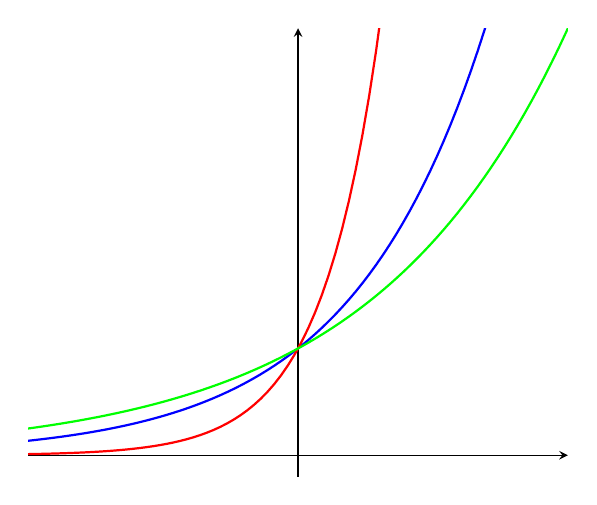
\begin{tikzpicture}
		\begin{axis}[xmin=-2,xmax=2,ymin=-0.2,ymax=4,axis x line=center,
		axis y line=center,ticks=none,restrict y to domain =0:20]
		\addplot[thick,blue, samples = 200] {exp(x)};
		\addplot[thick, red, samples = 200] {10^x};
		\addplot[thick, green, samples = 200] {2^x};
		\end{axis}
		\end{tikzpicture}
		\caption{Opgave~\ref{it:eks1}}
		\label{fig:eks1}
	\end{figure}


	\item Bestem halvveringskonstanten for funktionen $f(x)=e^{-2x}$
	
	
	\item Givet en eksponentialfunktion $f(x)=ba^x$ bestem $c$ og $d$ så $g(x)=cd^x$ er spejlingen af $f$ i $y$-aksen. (Hint: Symmetri om $y$-aksen er ensbetydende med at $f(-x)=g(x)$.)
	
	
	\item \label{it:eks2} Vis at 
	\begin{align*}
	\frac{\ln(a^y)}{\ln(a)}=y,\quad \textup{og}\quad a^{\frac{\ln(x)}{\ln(a)}}=x.
	\end{align*}
	Konkluder at
	\begin{align*}
	\log_a(x)=\frac{\ln(x)}{\ln(a)}.
	\end{align*}
	(Hint: til at vise den anden lighed brug at $ x=a^{\log_a(x)} $ på venstresiden.)
\end{enumerate}

\subsection{Trigonometriske funktioner}
\noindent Vi er nu kommet til at studere trigonometriske funktioner som sinus, cosinus og tangens. For at gøre dette vil vi starte med at betragte vinkler. Man kan måle vinkler i enten radianer eller grader, i dette kursus vil vi oftest benytte radianer, som er et mål for hvor langt man går på enhedscirklen. Vi har følgende sammenhæng mellem grader og radianer
\begin{align*}
2\pi \textup{ rad} = 360 \textup{ grader}
\end{align*}
hvilket medfører at 
\begin{align*}
1 \textup{ rad} = \frac{180}{\pi} \textup{ grader} \qquad \textup{ og } \qquad 1 \textup{ grader} = \frac{\pi}{180} \textup{ rad}.
\end{align*}
\paragraph*{Eksempler:}
\begin{enumerate}
\item Omskriv $2$ radianer til grader:

Vi har 
\begin{align*}
2 \textup{ rad} = 2 \cdot 1 \textup{ rad} = 2 \cdot \frac{180}{\pi} \textup{ grader} = \frac{360}{\pi} \textup{ grader}.
\end{align*}
\item Omskriv $280$ grader til radianer:

Vi har
\begin{align*}
280 \textup{ grader} = 280 \cdot 1 \textup{ grader} = 280 \cdot \frac{\pi}{180} \textup{ rad} = \frac{14\pi}{9} \textup{ rad}.
\end{align*}
\end{enumerate}
For at kunne definere de trigonometriske funktioner vil vi betragte enhedscirklen (se Figur~\ref{fig:funktioner5et}), som er en cirkel med radius $1$ og centrum i origo, som er punktet $(0,0)$.
\begin{figure}
\centering
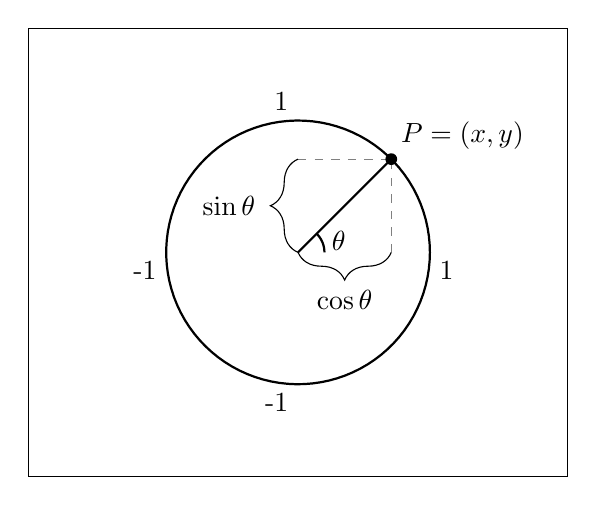
\begin{tikzpicture}
	\begin{axis}[xmin=-1.7,xmax=1.7,ymin=-1.7,ymax=1.7,ticks=none,axis equal]
	\addplot[domain=0:2*pi,thick, samples=100] ({cos(deg(x))},							{sin(deg(x))});
	\addplot[domain=0:sqrt(2)/2,thick] {1*x};
	\addplot[domain=0:pi/4,thick,samples=200] ({0.2*cos(deg(x))},						{0.2*sin(deg(x))})node[right,pos=0.6] {$\theta$};
	\node[above left] at (axis cs:0,1) {1};
	\node[below right] at (axis cs:1,0) {1};
	\node[below left] at (axis cs:0,-1) {-1};
	\node[below left] at (axis cs:-1,0) {-1};
	\draw[gray,dashed] (axis cs:{sqrt(2)/2},0) -- (axis cs:{sqrt(2)/2},{sqrt(2)/2});
	\draw[gray,dashed] (axis cs:0,{sqrt(2)/2}) -- (axis cs:{sqrt(2)/2},{sqrt(2)/2});
\draw [decorate,decoration={brace,amplitude=10pt}]
(axis cs:{sqrt(2)/2},0) -- (axis cs:0,0)node [below=10pt,midway] {$\cos\theta$};
\draw [decorate,decoration={brace,amplitude=10pt}]
(axis cs:0,0) -- (axis cs:0,{sqrt(2)/2})node [left=12pt,midway] {$\sin\theta$};
\node[fill,circle,inner sep=1.5pt] at (axis cs:{sqrt(2)/2},{sqrt(2)/2}){};
\node[above right] at (axis cs:{sqrt(2)/2},{sqrt(2)/2}){$P=(x,y)$};

\end{axis}
\end{tikzpicture}
\caption{Sinus og cosinus i enhedscirklen.}
\label{fig:funktioner5et}
\end{figure}
Hvis vi starter i punktet $(1,0)$ på enhedscirklen og bevæger os med en vinkel $\theta$ mod uret (se Figur~\ref{fig:funktioner5et}) så når vi til et punkt på enhedscirklen som vi kalder $P$. Hvis $P$ har koordinaterne $(x,y)$ så definerer vi $\cos\theta=x$ og $\sin\theta=y$. Hvis vi går imod urets retning i enhedscirklen, vil vi kalde det for den positive omløbsretning og hvis vi går i urets retning, vil vi kalde det for den negative omløbsretning.

Bemærk, at enhedscirklen er $2\pi$-periodisk. Det betyder, at hvis vi går en vinkel på $\theta$ mod uret og får et punkt $P$, så vil vi få det samme punkt hvis vi går vinklen $\theta+2\pi$, da der er $2\pi$ rundt om hele enhedscirklen. Det medfører også at sinus og cosinus er $2\pi$-periodiske funktioner, hvilket betyder at
\begin{align*}
\sin\theta = \sin(\theta + 2\pi k) \qquad \textup{ og } \qquad \cos\theta = \cos(\theta + 2\pi k),
\end{align*}
hvor $k$ er et heltal.

Hvis vi betragter Figur~\ref{fig:funktioner5to} ser vi, at hvis vi spejler et punkt $(x,y)$, på enhedscirklen, omkring $x$-aksen får vi punktet $(x,-y)$ på enhedscirklen. Da det at spejle et punkt omkring $x$-aksen er det samme som at gå vinklen i den negative omløbsretning, får vi at 
\begin{align*}
\sin(-\theta) = -\sin\theta \qquad \textup{ og } \qquad \cos(-\theta)=\cos\theta.
\end{align*}
På tilsvarende vis ser vi, at hvis vi spejler punktet $(x,y)$ i $y$-aksen får vi punktet $(-x,y)$. Da det at spejle i $y$-aksen, er det samme som at gå vinklen $\pi - \theta$ i positiv omløbsretning får vi, at
\begin{align*}
\sin(\pi - \theta)=\sin\theta \qquad \textup{ og } \qquad \cos(\pi - \theta) = - \cos\theta.
\end{align*} 
Vi definerer nu tangens ud fra sinus og cosinus, ved
\begin{align*}
\tan\theta=\frac{\sin\theta}{\cos\theta},
\end{align*}
når $\theta \neq \frac{\pi}{2} + \pi k$, hvor $k$ er et heltal. Tangens kan også bestemmes ud fra enhedscirklen (se Figur~\ref{fig:funktioner5tre}). Vi tegner en tangentlinje der skærer cirklen i punktet $(1,0)$. Hvis vi går en vinkel $\theta$ i enhedscirklen og så forlænger linjen indtil den skærer vores tangent, så er $\tan\theta$ præcis $y$-koordinaten i skæringspunktet. 
\begin{figure}[!htbp]
\begin{minipage}{0.49\textwidth}
\centering
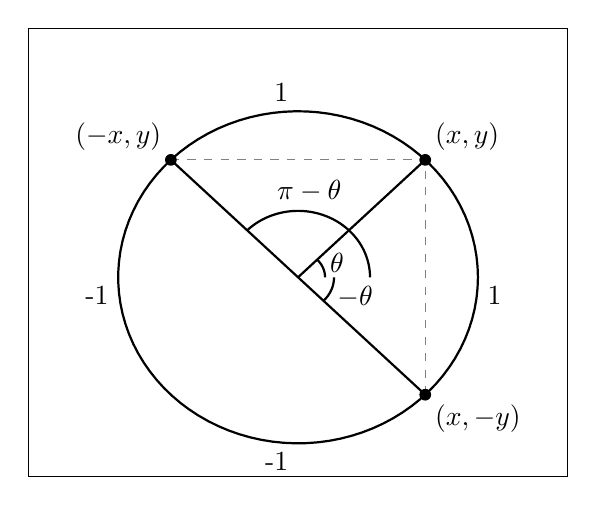
\begin{tikzpicture}
	\begin{axis}[xmin=-1.5,xmax=1.5,ymin=-1.2,ymax=1.5,ticks=none]
	\addplot[domain=0:2*pi,thick, samples=100] ({cos(deg(x))},							{sin(deg(x))});
	\addplot[domain=0:sqrt(2)/2,thick] {1*x};
	\addplot[domain=-sqrt(2)/2:sqrt(2)/2,thick] {-1*x};
	\addplot[domain=0:pi/4,thick,samples=200] ({0.15*cos(deg(x))},						{0.15*sin(deg(x))})node[right,pos=0.8] {$\theta$};
	\addplot[domain=0:-pi/4,thick,samples=200] ({0.2*cos(deg(x))},						{0.2*sin(deg(x))})node[right,pos=0.8] {$-\theta$};
	\addplot[domain=0:3*pi/4,thick,samples=200] ({0.4*cos(deg(x))},						{0.4*sin(deg(x))})node[above,pos=0.6] {$\pi-\theta$};
	\node[above left] at (axis cs:0,1) {1};
	\node[below right] at (axis cs:1,0) {1};
	\node[below left] at (axis cs:0,-1) {-1};
	\node[below left] at (axis cs:-1,0) {-1};
	\draw[gray,dashed] (axis cs:{sqrt(2)/2},{-sqrt(2)/2}) -- (axis cs:{sqrt(2)/2},{sqrt(2)/2});
	\draw[gray,dashed] (axis cs:{-sqrt(2)/2},{sqrt(2)/2}) -- (axis cs:{sqrt(2)/2},{sqrt(2)/2});
%\draw [decorate,decoration={brace,amplitude=10pt}]
%(axis cs:{sqrt(2)/2},0) -- (axis cs:0,0)node [below=10pt,midway] {$\mathrm  {cos}(\theta)$};
%\draw [decorate,decoration={brace,amplitude=10pt}]
%(axis cs:0,0) -- (axis cs:0,{sqrt(2)/2})node [left=12pt,midway] {$\mathrm  {sin}(\theta)$};
\node[fill,circle,inner sep=1.5pt] at (axis cs:{sqrt(2)/2},{sqrt(2)/2}){};
\node[above right] at (axis cs:{sqrt(2)/2},{sqrt(2)/2}){$(x,y)$};
\node[fill,circle,inner sep=1.5pt] at (axis cs:{sqrt(2)/2},{-sqrt(2)/2}){};
\node[below right] at (axis cs:{sqrt(2)/2},{-sqrt(2)/2}){$(x,-y)$};
\node[fill,circle,inner sep=1.5pt] at (axis cs:{-sqrt(2)/2},{sqrt(2)/2}){};
\node[above left] at (axis cs:{-sqrt(2)/2},{sqrt(2)/2}){$(-x,y)$};
\end{axis}
\end{tikzpicture}
\caption{Symmetrien i enhedscirklen.}
\label{fig:funktioner5to}
\end{minipage}
\begin{minipage}{0.49\textwidth}
 \centering
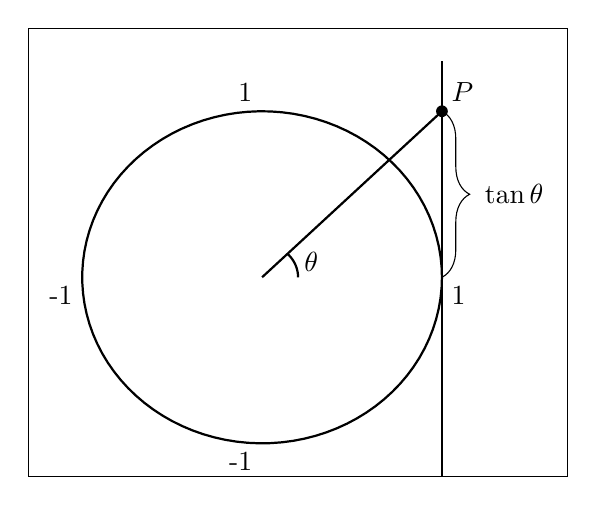
\begin{tikzpicture}
	\begin{axis}[xmin=-1.3,xmax=1.7,ymin=-1.2,ymax=1.5,ticks=none]
	\addplot[domain=0:2*pi,thick, samples=100] ({cos(deg(x))},							{sin(deg(x))});
	\addplot[domain=0:1,thick] {1*x};
	\addplot[domain=0:pi/4,thick,samples=200] ({0.2*cos(deg(x))},						{0.2*sin(deg(x))})node[right,pos=0.6] {$\theta$};
	\node[above left] at (axis cs:0,1) {1};
	\node[below right] at (axis cs:1,0) {1};
	\node[below left] at (axis cs:0,-1) {-1};
	\node[below left] at (axis cs:-1,0) {-1};
\draw[thick] (axis cs:1,-1.3) -- (axis cs:1,1.3);
\draw [decorate,decoration={brace,amplitude=10pt}]
(axis cs:1,1) -- (axis cs:1,0)node [right=12pt,midway] {$\tan\theta$};
\node[fill,circle,inner sep=1.5pt] at (axis cs:1,1){};
\node[above right] at (axis cs:1,1){$P$};
\end{axis}
\end{tikzpicture}
\caption{Tangens i enhedscirklen.}
\label{fig:funktioner5tre}
\end{minipage}
\end{figure}
\paragraph*{Trigonometriske identiter}
Vi opsummere her en liste over de trigonometriske identiteter vi har vist plus nogle flere som vil være brugbare i opgaveregningen:
\begin{enumerate}
\item $\cos(\theta + 2\pi k) = \cos(\theta)$, når $k$ er et heltal.
\item $\sin(\theta + 2\pi k) = \sin(\theta)$, når $k$ er et heltal.
\item $\sin(-\theta)=-\sin(\theta)$.
\item $\cos(-\theta)=\cos(\theta)$.
\item $\sin(\pi \pm \theta)=\mp \sin(\theta)$.
\item $\cos(\pi \pm \theta)=-\cos(\theta)$.
\item $\tan(\pi \pm \theta)=\pm \tan(\theta)$.
\item $\cos^2(\theta) + \sin^2(\theta)=1$ (Idiotformlen).
\item $\sin(\theta \pm \phi) = \sin(\theta)\cos(\phi)\pm\cos(\theta)\sin(\phi)$ (Additionsformlen for sinus).
\item $\cos(\theta \pm \phi) = \cos(\theta)\cos(\phi)\mp\sin(\theta)\sin(\phi)$ (Additionsformlen for cosinus).
\item $\cos(2\theta)=\cos^2(\theta)-\sin^2(\theta) = 2\cos^2(\theta)-1 = 1-2\sin^2(\theta)$.
\item $\sin(2\theta)=2\sin(\theta)\cos(\theta)$.
\end{enumerate}
Derudover giver vi en liste over værdierne for nogle udvalgte vinkler. Vi betragter her kun vinkler i første kvadrant, da vi kan finde værdier for de andre kvadranter ved at benytte de ovenstående formler.

\begin{table}[h!]
\centering
\begin{tabular}{l !{\qquad} {c}!{\qquad} {c}!{\qquad} r}
$\theta$           & $\sin \theta$ & $\cos \theta$ & $\tan \theta$  \\
\toprule
$0$				 & $0$ 				    & $1$  				   & $0$					\\ \midrule
$\displaystyle \frac{\pi}{6}$  & $\displaystyle\frac{1}{2}$        & $\displaystyle\frac{\sqrt{3}}{2}$ & $\displaystyle \frac{\sqrt{3}}{3}$   \\ \midrule
$\displaystyle\frac{\pi}{4}$  & $\displaystyle\frac{\sqrt{2}}{2}$	& $\displaystyle\frac{\sqrt{2}}{2}$ &	$1$					\\ \midrule
$\displaystyle\frac{\pi}{3}$  & $\displaystyle\frac{\sqrt{3}}{2}$ & $\displaystyle\frac{1}{2}$		   & $\sqrt{3}$				\\ \midrule
$\displaystyle\frac{\pi}{2}$  & $1$ 			        & $0$				   &   \\
\bottomrule  
\end{tabular}
\caption{Værdier for udvalgte vinkler}\label{tab:funktioner5et}
\end{table}

\paragraph*{Eksempler:}
\begin{enumerate}
\item Beregn værdien $\cos(\frac{3\pi}{2})$:

Ved at bruge den trigonometriske identitet nummer $6.$ får vi at
\begin{align*}
\cos\Big( \frac{3\pi}{2}\Big) = \cos\Big(\pi + \frac{\pi}{2}\Big) = -\cos\Big(\frac{\pi}{2} \Big)=-0=0.
\end{align*}
\item Beregn $\sin(9\pi)$:

Ved at bruge den trigonometriske identitet nummer $2.$ får vi at
\begin{align*}
\sin(9\pi)=\sin(\pi + 8\pi)= \sin(\pi + 2 \cdot 4 \cdot \pi) = \sin(\pi) = 0.
\end{align*}
\item Vis at den trigonometriske identitet nummer $5$. gælder for plus, ved at bruge additionsformlen for sinus:

Vi sætter $\phi=\pi$ i additionsformlen for sinus og får
\begin{align*}
\sin(\theta+\pi) = \sin(\theta)\cos(\pi)+\cos(\theta)\sin(\pi).
\end{align*}
Vi ser i enhedscirklen at~\ref{tab:funktioner5et} at $\cos(\pi)=-1$ og $\sin(\pi)=0$. Indsætter vi det i den ovenstående ligning får vi at
\begin{align*}
\sin(\theta+\pi) = \sin\theta\cdot (-1)+\cos\theta\cdot 0 =-\sin\theta.
\end{align*}
\end{enumerate}
\subsection{Opgaver}

\begin{enumerate}
	\item Omregn følgende fra grader til radianer
	\begin{align*}
	90^\circ,&& 15^\circ,&&150^\circ,&& 45^\circ.
	\end{align*}
	
	\item Omregn følgende radianer til grader
	\begin{align*}
	\frac{\pi}{3},&&\frac{7\pi}{4},&& \frac{5\pi}{12}.
	\end{align*}
	

	
		\item Brug \href{https://www.geogebra.org/m/e2vTM4Ut}{GeoGebra} til at undersøge de trigonometriske funktioner sinus og cosinus. Bemærk at GeoGebra laver nogle afrundinger der kræver at man bruger sund fornuft når man aflæser funktionerne.
	\begin{enumerate}
		\item Bestem $\sin(0)$ og $\cos(0)$.
		\item Bestem $\sin(\frac{\pi}{2})$ og $ \cos(\frac{\pi}{2}) $.
		\item Bestem $\sin(\pi)$ og $\cos(\pi)$.
		\item Bestem $\sin(\frac{3\pi}{2}) $ og $\cos(\frac{3\pi}{2})$.
		\item Bestem $\sin(2\pi)$ og $ \cos(2\pi) $.
	\end{enumerate}
	
	 \item Udregn følgende tal
	\begin{align*}
	\sin(\frac{5\pi}{4})+\cos(\frac{\pi}{4}),&& \tan(\frac{\pi}{6})+\cos(\frac{\pi}{3}),&& \frac{\sin(\frac{\pi}{6})+\cos(\frac{\pi}{3})}{\sin(\frac{4\pi}{6})}.
	\end{align*}
	
	\begin{figure}
		\centering
		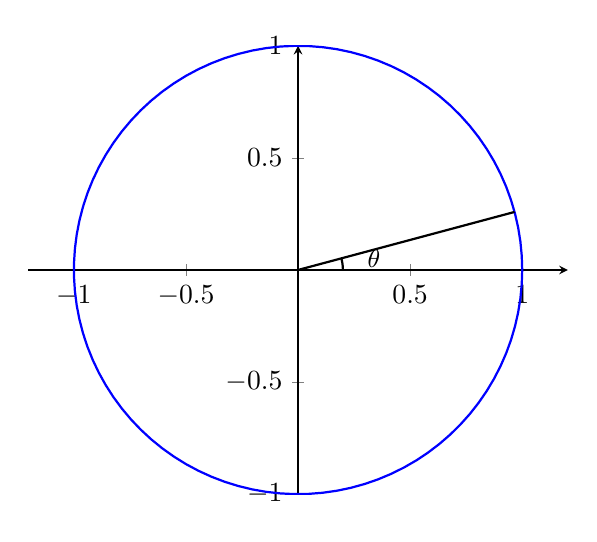
\begin{tikzpicture}
		\begin{axis}[xmin=-1,xmax=1,ymin=-1,ymax=1,axis x line=center,
		axis y line=center, axis equal]
		\addplot[blue,domain=0:2*pi,thick, samples=100] ({cos(deg(x))},{sin(deg(x))});
		\addplot[domain=0:(sqrt(6)+sqrt(2))/4,thick] {(2-sqrt(3))*x};
		\addplot[domain=0:pi/12,thick,samples=100] ({0.2*cos(deg(x))},{0.2*sin(deg(x))}) node[label={[label distance=2pt]0.5:\small$\theta$},pos=1] {};
		\end{axis}
		\end{tikzpicture}
		\caption{Opgave~\ref{it:trig1}}
		\label{fig:trig1}
	\end{figure}
	

	\item Brug sumformlerne til at vise formlerne $\sin(-\theta)=-\sin(\theta) $ og $\cos(-\theta)=\cos(\theta) $. Se evt. \href{https://www.geogebra.org/m/e2vTM4Ut}{GeoGebra}. (Hint $\cos(-\theta)=\cos(0-\theta)$ og $\sin(-\theta)=\sin(0-\theta)$).
	
	\item Brug \href{https://www.geogebra.org/m/e2vTM4Ut}{GeoGebra} til at formode en sammenhæng mellem $\cos(\theta-\frac{\pi}{2})$ og $\sin(\theta)$. Brug efterfølgende sumformlerne til at be- eller afkræfte formodningen.
	  
	  	\item \label{it:trig1} I Figur~\ref{fig:trig1} er en vinkel på $\theta$ indtegnet i enhedscirklen. Skitser vinklerne
	  \begin{align*}
	  \theta+ \frac{\pi}{2},&& \pi-\theta,&& \theta +3\pi,&& \frac{7\pi}{4}-\theta.
	  \end{align*}
	  
	
	 
	 \item Bestem to forskellige løsninger til ligningerne 
	 \begin{align*}
	 \sin(x)=\frac{\sqrt{3}}{2},&& \cos(x-\pi)=-\frac{\sqrt{2}}{2},&& 2\sin^2(x)+5\sin(x)+2=0.
	 \end{align*}

	\item Brug enhedscirklen til at vise idiotformlen
	\begin{align*}
	\sin^2x+\cos^2x=1.
	\end{align*}
	(Hint: Pythagoras.)

	\item Udregn følgende
	\begin{align*}
	\cos(-\frac{3\pi}{4}),&& \sin(\frac{5\pi}{6}),&&\tan(\frac{5\pi}{4}),&& \cos(\frac{5\pi}{3}).
	\end{align*}
	
	\item\label{it:trig2} Vis at $\sin(2\theta)=2\cos(\theta)\sin(\theta)$. (Hint: Brug sumformlerne)

	\item Løs ligningen $16\sin^2(x)\cos^2(x)=3$ for $x\in [0,\pi]$. (Hint: Brug formlen fra Opgave~\ref{it:trig2})
	
	\item Udregn
	\begin{align*}
	\cos(\frac{15\pi}{4}),&& \tan(\frac{14\pi}{6}),&& \sin(-\frac{10\pi}{3}),&& \tan(\frac{10 \pi}{5}).
	\end{align*}
	
	\item Vis at $\tan(x+\pi)=\tan(x)$ for alle hvor tangens er defineret. (Hint: Brug sumformlerne.)
	
	\item Løs ligningen $\sin^2(\theta)+3\cos^2(\theta) =2$ for $\theta\in [0,\frac{\pi}{2}]$.(Hint: Idiotformlen)
	
	\item \label{it:trig3} I denne opgave beviser vi nogle af de eksakte værdier for sinus og cosinus til vinklerne $ \frac{\pi}{6}$ og $ \frac{\pi}{6} $.
	
	\begin{enumerate}
		\item Vis at $\sin(\frac{\pi}{6})=\frac{1}{2}$ ved at regne på trekanten i Figur~\ref{fig:trig3}. (Hint: Hvad kan man sige om sidelængderne i trekanten?)
		
		\item Brug idiotformlen til at vise at $\cos(\frac{\pi}{6})=\frac{\sqrt{3}}{2}$.
		
		\item Vis at $\sin(\frac{\pi}{3})=\frac{\sqrt{3}}{2}$. (Hint: $ \sin(\frac{\pi}{3})=\sin(\frac{\pi}{6}+\frac{\pi}{6}) $)
		
		\item Brug idiotformlen til at vise at $\cos(\frac{\pi}{3})=\frac{1}{2}$.
		
	\end{enumerate}
		
	\begin{figure}
		\centering
		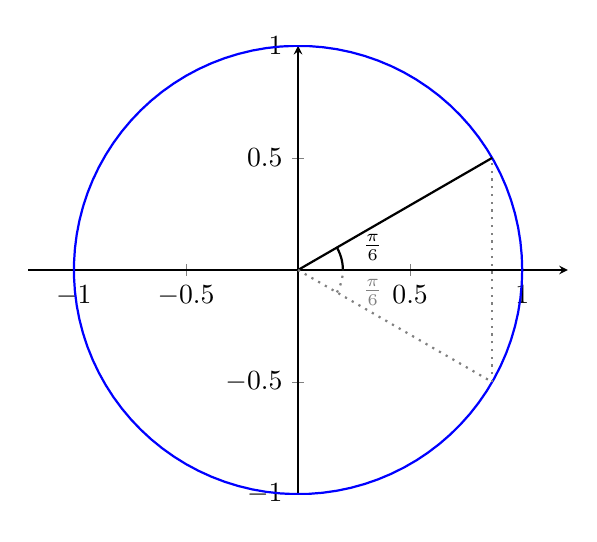
\begin{tikzpicture}
		\begin{axis}[xmin=-1,xmax=1,ymin=-1,ymax=1,axis x line=center,
		axis y line=center, axis equal]
		\addplot[blue,domain=0:2*pi,thick, samples=100] ({cos(deg(x))},{sin(deg(x))});
		\addplot[domain=0:sqrt(3)/2,thick] {1/sqrt(3)*x};
		\addplot[domain=0:pi/6,thick,samples=100] ({0.2*cos(deg(x))},{0.2*sin(deg(x))}) node[label={[label distance=2pt]0.5:\small$\frac{\pi}{6}$},pos=1] {};
		\addplot[domain=0:sqrt(3)/2,thick,gray,dotted] {-1/sqrt(3)*x};
		\addplot[domain=-pi/6:0,thick,samples=100,gray,dotted] ({0.2*cos(deg(x))},{0.2*sin(deg(x))}) node[label={[label distance=2pt]0.5:\small$\frac{\pi}{6}$},pos=0] {};
		\addplot[dotted,gray,thick] coordinates {(sqrt(3)/2, -1/2) (sqrt(3)/2, 1/2)};
		\end{axis}
		\end{tikzpicture}
		\caption{Opgave~\ref{it:trig3}}
		\label{fig:trig3}
	\end{figure}

		\item \label{it:trig4} I denne opgave beviser vi nogle af de eksakte værdier for sinus og cosinus til vinklerne $ \frac{\pi}{4}$.
		\begin{enumerate}
			\item Vis at $\sin(\frac{\pi}{4})=\frac{\sqrt{2}}{2}$ ved at regne på trekanten i Figur~\ref{fig:trig4}.(Hint: Pythagoras) 
			\item Brug idiotformlen til at vise at $\cos(\frac{\pi}{4})=\frac{\sqrt{2}}{2}$. 
		\end{enumerate}
	
	\begin{figure}
		\centering
		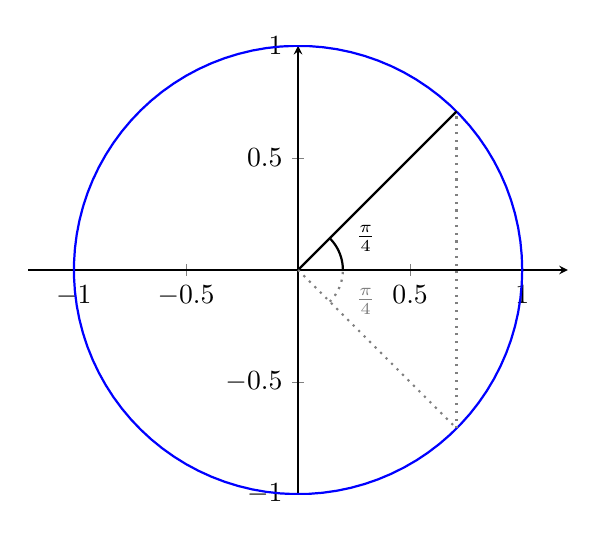
\begin{tikzpicture}
		\begin{axis}[xmin=-1,xmax=1,ymin=-1,ymax=1,axis x line=center,
		axis y line=center, axis equal]
		\addplot[blue,domain=0:2*pi,thick, samples=100] ({cos(deg(x))},{sin(deg(x))});
		\addplot[domain=0:sqrt(2)/2,thick] {1*x};
		\addplot[domain=0:pi/4,thick,samples=100] ({0.2*cos(deg(x))},{0.2*sin(deg(x))}) node[label={[label distance=2pt]0.5:\small$\frac{\pi}{4}$},pos=1] {};
		\addplot[domain=0:sqrt(2)/2,thick,gray,dotted] {-1*x};
		\addplot[domain=-pi/4:0,thick,samples=100,gray,dotted] ({0.2*cos(deg(x))},{0.2*sin(deg(x))}) node[label={[label distance=2pt]0.5:\small$\frac{\pi}{4}$},pos=0] {};
		\addplot[dotted,gray,thick] coordinates {({sqrt(2)/2}, -{sqrt(2)/2}) ({sqrt(2)/2}, {sqrt(2)/2})};
		\end{axis}
		\end{tikzpicture}
		\caption{Opgave~\ref{it:trig4}}
		\label{fig:trig4}
	\end{figure}

	\item \label{it:trig5}I denne opgave beviser vi nogle af de eksakte værdier for sinus og cosinus til vinklerne $ \frac{\pi}{12}$ og $ \frac{5\pi}{12} $.
	\begin{enumerate}
%		\item Brug Figur~\ref{fig:trig5} at $\sin(\frac{\pi}{12})=\frac{\sqrt{2-\sqrt{3}}}{2}$. (Hint: Brug cosinusrelationen)
%		\item Brug idiotformlen til at bestemme $\cos(\frac{\pi}{12})$. 
		\item Bestem $\cos(\frac{\pi}{12})$ og $\sin(\frac{\pi}{12})$ ved at bruge sumformlerne. (Hint: $ \frac{\pi}{12}=\frac{\pi}{3}-\frac{\pi}{4} $)
		\item  Bestem $\cos(\frac{5\pi}{12})$ og $\sin(\frac{5\pi}{12})$ ved at bruge sumformlerne. (Hint: $ \frac{5\pi}{12}=\frac{\pi}{6}+\frac{\pi}{4} $)
	\end{enumerate}
	
	
%	\begin{figure}
%		\centering
%		\begin{tikzpicture}
%		\begin{axis}[xmin=-1,xmax=1,ymin=-1,ymax=1,axis x line=center,
%		axis y line=center, axis equal]
%		\addplot[blue,domain=0:2*pi,thick, samples=100] ({cos(deg(x))},{sin(deg(x))});
%		\addplot[domain=0:(sqrt(6)+sqrt(2))/4,thick] {(2-sqrt(3))*x};
%		\addplot[domain=0:pi/12,thick,samples=100] ({0.2*cos(deg(x))},{0.2*sin(deg(x))}) node[label={[label distance=2pt]0.5:\tiny$\frac{\pi}{12}$},pos=1] {};
%
%		\addplot[domain=0:(sqrt(6)+sqrt(2))/4,thick,gray,dotted] {-(2-sqrt(3))*x};
%		\addplot[domain=-pi/12:0,thick,samples=100,gray,dotted] ({0.2*cos(deg(x))},{0.2*sin(deg(x))}) node[label={[label distance=2pt]0.5:\tiny$\frac{\pi}{12}$},pos=0] {};
%		\addplot[dotted,gray,thick] coordinates {({(sqrt(6)+sqrt(2))/4}, -{(sqrt(6)-sqrt(2))/4}) ({(sqrt(6)+sqrt(2))/4}, {(sqrt(6)-sqrt(2))/4})};
%		\end{axis}
%		\end{tikzpicture}
%		\caption{Opgave~\ref{it:trig5}}
%		\label{fig:trig5}
%	\end{figure}
%	

	
\end{enumerate}

\section{Grænseværdier og kontinuitet}
\noindent Når vi senere vil snakke om differentiabilitet, vil vi snakke om at tage grænsen af sekanthældningen, men hvad mener vi med at tage ``grænsen'', det vil vi nu specificere. Vi siger at $f(x)$ har en grænseværdi $L^-$ fra venstre for $x$ gående mod $a$ fra venstre og noterer det med
\begin{align*}
\lim_{x \to a^-} f(x) = L^-,
\end{align*}
hvis $f(x)$ kan komme lige så tæt på $L^-$ som vi ønsker, ved at lade $x$ komme tættere og tættere på $a$ fra venstre. På tilsvarende vis siger vi, at $f(x)$ har en grænseværdi $L^+$ fra højre for $x$ gående mod $a$ fra højre og notere det med 
\begin{align*}
\lim_{x \to a^+} f(x) = L^+.
\end{align*}
Hvis der gælder at 
\begin{align*}
\lim_{x \to a^-} f(x)=L^-=L^+=\lim_{x \to a^+} f(x),
\end{align*}
så siger vi, at $f(x)$ har en grænseværdi $L$ for $x$ gående mod $a$ og notere det med
\begin{align*}
\lim_{x \to a } f(x) =L.
\end{align*}
Konceptet med en grænseværdi er ikke let at forstå, derfor illustrerer vi det nu ved hjælp af figurer, og dernæst med nogle simple eksempler. Hvis vi betragter Figur~\ref{fig:graenseret} ser vi, at hvis vi lader $x$ nærme sig $a$ fra henholdsvis højre og venstre så vil vi få
\begin{align*}
\lim_{x \to a^-} f(x)=L \qquad \textup{ og } \qquad \lim_{x \to a^+} f(x)=L,
\end{align*}
hvilket medfører at funktionen $f$ har en grænseværdi i $a$ som er
\begin{align*}
\lim_{x \to a} f(x) =L.
\end{align*}
Hvis vi derimod betragter Figur~\ref{fig:graenserto}, ser vi at 
\begin{align*}
\lim_{x \to a^-} f(x)=L^- \qquad \textup{ og } \qquad \lim_{x \to a^+}=L^+,
\end{align*}
hvor $L^- \neq L^+$. Det betyder at grænsen fra højre og grænsen for venstre ikke er lig med hinanden i punktet $a$, og dermed har $f$ ikke en grænseværdi for $x$ gående mod $a$.

Bemærk, at man kan godt snakke om $f$ har en grænseværdi for $x$ gående mod $a$ selvom $f(a)$ slet ikke er defineret.
\begin{figure}[!htbp]
\begin{minipage}{0.49\textwidth}
\centering
\begin{tikzpicture}
	\begin{axis}[xmin=-1.5,xmax=1.5,ymin=-1.5,ymax=1.5,ticks=none,restrict y to domain=-1.5:1.5]
	\addplot[thick, samples=100,domain=-1.1:1.1] {x^3};
	\draw[dashed] (axis cs:1,0) -- (axis cs:1,1);	
	\node[below] at (axis cs:1,0){$a$};
	\draw[dashed] (axis cs:0,1) -- (axis cs:1,1);	
	\node[left] at (axis cs:0,1){$L^-=L^+=L$};
	\node[above left=3 pt] at (axis cs:1.1,1.1){$f(x)$};
\end{axis}
\end{tikzpicture}
\caption{Grænseværdi i $x=a$.}
\label{fig:graenseret}
\end{minipage}
\begin{minipage}{0.49\textwidth}
 \centering
\begin{tikzpicture}
	\begin{axis}[xmin=-1.3,xmax=1.7,ymin=-1.2,ymax=1.5,ticks=none,restrict y to domain=-1:1.5]
	\addplot[domain=-1.1:1,thick, samples=100] {x^2};
	\addplot[domain=1:10,thick, samples=100] {-x+2.3};
	\draw[dashed] (axis cs:1,0) -- (axis cs:1,1);	
	\node[below] at (axis cs:1,0){$a$};
	\draw[fill] (axis cs:1,1) circle[radius=0.1em];
	\draw[fill=white] (axis cs:1,1.3) circle[radius=0.1em];
	\node[above right] at (axis cs:-1.1,1.2){$f(x)$};
	\draw[dashed] (axis cs:0,1) -- (axis cs:1,1);	
	\node[left] at (axis cs:0,1){$L^-$};
	\draw[dashed] (axis cs:0,1.3) -- (axis cs:1,1.3);	
	\node[left] at (axis cs:0,1.3){$L^+$};
\end{axis}
\end{tikzpicture}
\caption{Ingen grænseværdi i $x=a$.}
\label{fig:graenserto}
\end{minipage}
\end{figure}

\paragraph*{Eksempler:}
\begin{enumerate}
\item Lad $f(x)=x^3$ og vis at $f$ har en grænseværdi for $x$ gående mod $2$ og bestem denne.

Vi ser, at vi kan lade $f(x)$ komme lige så tæt på $8$ som vi ønsker ved at lade $x$ komme tættere og tættere på $2$ fra både højre og venstre, hvilket medfører at
\begin{align*}
\lim_{x \to 2^-} f(x) = 8 \qquad \textup{ og } \qquad \lim_{x \to 2^+} f(x) = 8.
\end{align*}
Da grænsen fra højre og venstre er den samme har vi 
\begin{align*}
\lim_{x \to 2} x^3=8.
\end{align*}
\item Har funktionen
\begin{align*}
f (x) = 
\begin{cases}
x^2 & \textup{ hvis } x \leq 1, \\
-x+3 & \textup{ hvis } x > 1,
\end{cases}
\end{align*}
en grænseværdi for $x$ gående mod $1$?

Vi forklarer først kort hvad vi mener med den måde $f$ er defineret på. Hvis vores $x$-værdi er mindre eller lig $1$ så er $f(x)=x^2$, mens vi for alle $x$-værdier der er skarpt større end $1$ har at $f(x)=-x+3$. Hvis $f$ er givet på denne måde, siger man, at $f$ er en gaffelfunktion.

Vi finder grænsen for $f(x)$ når $x$ går mod $1$ fra henholdsvis venstre og højre
\begin{align*}
\lim_{x \to 1^-} f(x) = \lim_{x \to 1^-} x^2 = 1 \qquad \textup{ og } \qquad \lim_{x \to 1^+} f(x)= \lim_{x \to 1^+} -x+3 = 2, 
\end{align*} 
da $f(x)=x^2$ kan komme vilkårligt tæt på $1$ ved at lade $x$ komme tættere og tættere på $1$ og tilsvarende kan vi lade $f(x)=-x+3$ komme vilkårligt tæt på $2$. Da
\begin{align*}
\lim_{x \to 1^-} f(x) \neq \lim_{x \to 1^+} f(x),
\end{align*}
har $f$ ikke en grænseværdi for $x$ gående mod $1$.
\end{enumerate}
\paragraph*{Regneregler:}
Lad $f$ og $g$ være to funktioner med grænseværdier når $x$ går mod $a$. Så har vi følgende regneregler for grænseværdierne:
\begin{enumerate}
\item $\displaystyle\lim_{x \to a} (f+g)(x) = \displaystyle\lim_{x \to a} f(x) + \lim_{x \to a} g(x)$.
\item $\displaystyle\lim_{x \to a} cf(x) = c \displaystyle\lim_{x \to a} f(x)$, hvor $c \in \mathbb{R}$.
\item $\displaystyle\lim_{x \to a} (fg)(x) = \displaystyle\lim_{x \to a} f(x) \cdot \lim_{x \to a} g(x)$.
\item $\displaystyle \lim_{x \to a} \Big(\frac{f}{g}\Big)(x) = \frac{\displaystyle\lim_{x \to a} f(x)}{\displaystyle\lim_{x \to a} g(x)}$, hvis $\displaystyle\lim_{x \to a} g(x) \neq 0$.
\end{enumerate}

\paragraph*{Kontinuitet:}
En funktion $f$ siges at være kontinuert i punktet $a$, hvis
\begin{align}\label{eq:graenserkontinuitetet}
\lim_{x \to a} f(x) = f(a).
\end{align}
Det betyder, at $f$ er kontinuert i $a$ hvis den har en grænseværdi i punktet $a$ der er lig med $f(a)$.

Vi siger, at $f$ er en kontinuert funktion, hvis den er kontinuert i alle punkter i dens definitionsmængde.  

Hvis $f$ og $g$ er kontinuerte funktioner, så har vi fra \eqref{eq:graenserkontinuitetet}, at
\begin{align*}
\lim_{x \to a} f(g(x)) = f(\lim_{x \to a} g(x)) = f(g(a)).
\end{align*}
Bemærk, at funktioner så som $x,ax+b,ax^2+bx+c,\frac{1}{x},\sqrt{x},\ln(x), e^x, \sin(x),\cos(x)$ alle er kontinuerte på passende domæne.

\paragraph*{Eksempler:}
\begin{enumerate}
\item Vis at funktionen 
\begin{align*}
f(x)=
\begin{cases}
2x+3 & x \neq 0, \\
3 & x=0,
\end{cases}
\end{align*}
er kontinuert i $0$.

Vi finder først grænseværdien for $f$ når $x$ går mod $0$, ved at finde grænseværdien fra henholdsvis venstre og højre
\begin{align*}
\lim_{x \to 0^-} f(x) = \lim_{x \to 0^-} 2x+3=3 \qquad \textup{ og } \qquad \lim_{x \to 0^+} f(x) = \lim_{x \to 0^+} 2x+3 = 3,
\end{align*}
hvilket medfører at $\displaystyle\lim_{x \to 0} f(x) = 3$.

Vi ser derudover at $f(0)=3$, så 
\begin{align*}
\lim_{x \to 0} f(x) = 3 = f(0),
\end{align*}
hvilket betyder at $f$ er kontinuert i $0$.
\item Vis at funktionen 
\begin{align*}
f(x)=
\begin{cases}
2x+3 & x \neq 0, \\
4 & x=0,
\end{cases}
\end{align*}
ikke er kontinuert i $0$.

Vi har fra den forrige opgave at $\lim_{x \to 0} f(x)=3$ men da $f(0) = 4$, har vi at
\begin{align*}
\lim_{x \to 0} f(x) \neq f(0),
\end{align*}
og dermed er $f$ ikke kontinuert i $0$.
\end{enumerate}









\subsection{Opgaver}

\begin{enumerate}
	\item Lad $f\colon \R\to \R$ være givet ved
	\begin{align*}
	f(x)=\begin{cases}
	2x+3,& \textup{hvis } x\neq 1\\
	6,&\textup{ellers}.
	\end{cases}
	\end{align*}
	Bestem $\lim_{x\to 1}f(x)$, $f(1)$ og afgør om $f$ er kontinuert.
	
	
	\item Lad $f\colon \R\to \R$ være givet ved
	\begin{align*}
	f(x)=\begin{cases}
	2x^2-1,& \textup{hvis } x\neq 2\\
	7,&\textup{ellers}.
	\end{cases}
	\end{align*}
	Bestem $\lim_{x\to 2}f(x)$ og afgør om $f$ er kontinuert.

	
	
	\item Bestem de følgende grænseværdier
	\begin{align*}
	\lim_{x\to 3} x^2,&& \lim_{x\to 0} \frac{1}{x-1},&&\lim_{x\to -2} \frac{x^2-4}{x+2},&& \lim_{x\to 0} \frac{-2\frac{1}{x^3}-4\frac{1}{x^2}+12}{3\frac{1}{x^3}+\frac{1}{x}}
	\end{align*}
	


	
	
	\item Lad $f\colon \R\to \R$ være givet ved
	\begin{align*}
	f(x)=\begin{cases}
	\frac{1}{3}x+\frac{7}{6}, & \textup{hvis } x<-\frac{1}{2}\\
	-\frac{2}{3}x^2-\frac{1}{3}x+1,& \textup{hvis } x\geq -\frac{1}{2}.
	\end{cases}	
	\end{align*}
	Bestem grænsen $\lim_{x\to -\frac{1}{2}} f(x)$ såfremt den er veldefineret. 
	
	\item Lad funktionen $f\colon \R\to \R$ være givet ved
	\begin{align*}
	f(x)=\begin{cases}
	x^3+x-1,&\textup{hvis } x<1\\
	4x^4-2x^2+1,&\textup{hvis } x>1\\
	2,& \textup{ellers}.
	\end{cases}
	\end{align*}
	Hvad er $f(1)$? Er $f$ kontinuert i $1$.
	
	
	\item Bestem $a$ og $b$ så funktionen
	\begin{align*}
	f(x)=\begin{cases}
	ax,&\textup{hvis } x<1\\
	5,&\textup{hvis } x=1\\
	bx^2+x+1,& \textup{hvis }x>1
	\end{cases}
	\end{align*}
	er kontinuert i $1$.
	
	\item\label{it:lim2} Lad $f\colon \R\to \R$ være givet ved
	\begin{align*}
	f(x)=\begin{cases}
	\frac{x}{\abs{x}},&\textup{hvis } x\neq 0\\
	0 ,& \textup{ellers}.
	\end{cases}
	\end{align*}
	Bestem $ f(0) $, $ \lim_{x\to 0^+}f(x) $ og $\lim_{x\to 0^-}f(x)$. I hvilke punkter er $f$ kontinuert?
	
	\item Bestem grænserne
	\begin{align*}
	\lim_{x\to 2} \frac{x^2+4-4x}{x^2-4},&& \lim_{x\to -5} \frac{(x-1)(2x^2+14x+20)}{x^2+4x-5}
	\end{align*}
	
	\item Lad $f$ være givet som i Opgave~\ref{it:lim2} og lad $g(x)=-f(x)$. 
	\begin{enumerate}
		\item Bestem $ (f+g)(0) $, $ \lim_{x\to 0^+}(f+g)(x) $ og $\lim_{x\to 0^-}(f+g)(x)$. I hvilke punkter er $(f+g)$ kontinuert?
		\item Bestem $ (fg)(0) $, $ \lim_{x\to 0^+}(fg)(x) $ og $\lim_{x\to 0^-}(fg)(x)$. I hvilke punkter er $(fg)$ kontinuert?
	\end{enumerate}
	
	\item Funktionen $f\colon \R\to \R$ givet ved 
	\begin{align*}
	f(x)=\begin{cases}
	2x^2+x+1,&\textup{hvis } x\in [-a,a]\\
	x+2,&\textup{ellers}
	\end{cases}
	\end{align*}
	er plottet i \href{https://www.geogebra.org/m/mAmaHPC6}{Geogebra}.
	\begin{enumerate}
		\item Bestem $a>0$ så $f$ er kontinuert.
		\item Er $f$ kontinuert når $a=0$?
	\end{enumerate}

	\item Bestem grænserne
	\begin{align*}
	\lim_{x\to 1} \frac{\ln x}{x},&& \lim_{x\to -2} (x^2-x)e^{x^2},&&  \lim_{x\to -1} x\ln(x+3).
	\end{align*}
	
	\item\label{it:lim1} I denne opgave bestemmes grænseværdien for funktionen $\frac{\sin x}{x}$ når $x$ går mod nul.
	\begin{enumerate}
		\item Figur~\ref{fig:lim1} viser vinklen $x\in [0,\frac{\pi}{2}[$ indtegnet i enhedscirklen. Brug figuren til at vise uligheden
		\begin{align*}
		\frac{1}{2}\sin x\leq \frac{1}{2}x\leq \frac{1}{2}\tan x.
		\end{align*}
		(Hint: Sammenlign arealet af det grå cirkeludsnit med arealet af $\Delta ACD$ og $\Delta ABD$ ).
		\item Omskriv uligheden fra (a) til 
		\begin{align*}
		\cos(x)\leq \frac{\sin x}{x}\leq 1.
		\end{align*}
		\item Brug at $\lim_{x\to 0} \cos(x)=1$ samt uligheden i (b) til at argumentere for at
		\begin{align*}
		\lim_{x\to 0}\frac{\sin x}{x}=1
		\end{align*}
	\end{enumerate}
	
	\begin{figure}
		\centering
		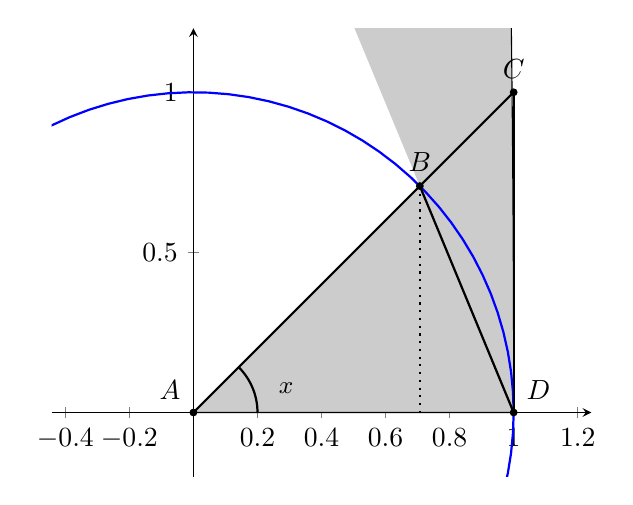
\begin{tikzpicture}
		\begin{axis}[xmin=-0.2,xmax=1,ymin=-0.2,ymax=1.2,axis x line=center,
		axis y line=center, axis equal]
				\pgfmathsetmacro\foo{sqrt(2)/2}
		\draw[fill=gray!40] (axis cs:0,0)--(axis cs:1,0)--(axis cs:\foo,\foo);		
		\draw[fill=gray!40] (axis cs:1,0)  arc[start angle=0, end angle=45,radius={transformdirectionx(1)}];

		\addplot[blue,domain=0:2*pi,thick, samples=100] ({cos(deg(x))},{sin(deg(x))});
		\addplot[domain=0:1,thick] {x};
		\addplot[domain=0:pi/4,thick,samples=100] ({0.2*cos(deg(x))},{0.2*sin(deg(x))}) node[label={[label distance=2pt]0:\small$x$},pos=0.5] {};
		\addplot[dotted,thick] coordinates {({sqrt(2)/2}, {sqrt(2)/2}) ({sqrt(2)/2}, 0)};
		\addplot[domain=sqrt(2)/2:1,thick] {{-x*sqrt(2)/(2-sqrt(2))+sqrt(2)/(2-sqrt(2))}};
		\addplot[thick] coordinates {(1,1) (1,0) };
		
		\node[fill, circle, inner sep=1pt] at (axis cs:0,0) [label=above left: $A$]{};
		\node[fill, circle, inner sep=1pt] at (axis cs:\foo,\foo) [label=above: $B$]{};
		\node[fill, circle, inner sep=1pt] at (axis cs:1,1) [label=above: $C$]{};
		\node[fill, circle, inner sep=1pt] at (axis cs:1,0) [label=above right: $D$]{};
		\end{axis}
		\end{tikzpicture}
		\caption{Opgave~\ref{it:lim1}}
		\label{fig:lim1}
	\end{figure}

	\item\label{it:lim3} Vis at 
	\begin{align*}
	\lim_{x\to 0}\frac{\cos (x)-1}{x}=0.
	\end{align*} 
	(Hint: Bruge Opgave~\ref{it:lim1}, identiteten
	\begin{align*}
	\frac{\cos (x)-1}{x}=\frac{\sin^2 x}{x(1+\cos x)}= \frac{\sin x}{x}\frac{\sin x}{1+\cos x}
	\end{align*}
	og produktreglen for grænser.)
	
	\item \label{it:lim4} Brug Opgave~\ref{it:lim1} del (b) til at vise at
	\begin{align*}
	\frac{\cos(x)-1}{x}\leq \frac{\sin(x)-x}{x^2}\leq 0.
	\end{align*}
	Argumenter vha. Opgave~\ref{it:lim3} for at 
	\begin{align*}
	\lim_{x\to 0}\frac{\sin(x)-x}{x^2}=0.
	\end{align*}
	
	\item\label{it:lim5} Vis at 
	\begin{align*}
	\lim_{x\to 0}\frac{\cos (x)-1}{x^2}=\frac{1}{2}.
	\end{align*} 
	(Hint: Bruge Opgave~\ref{it:lim1}, identiteten
	\begin{align*}
	\frac{\cos (x)-1}{x^2}=\frac{\sin^2 x}{x^2(1+\cos x)}= \Big(\frac{\sin x}{x}\Big)^2\frac{1}{1+\cos x}
	\end{align*}
	og produktreglen for grænser.)	
		
	
\end{enumerate}

\chapter{Differentiabilitet}
\section{Differentialkvotienter og differentialregneregler}
\noindent Differentialregning omhandler at bestemme hældningen af en funktion $f$. Vi definerer hældningen af et punkt til at være
\begin{align}\label{eq:diff1et}
f'(x_0) = \lim_{h \to 0} \frac{f(x_0+h)-f(x_0)}{h},
\end{align}
hvor $f'(x_0)$ kaldes differentialkvotienten i punktet $x_0$. Dette betyder, at vi skal finde grænsen fra både højre og venstre.

Motivationen for dette er, at vi tidligere kiggede på hældningen for en ret linje og hvis vi har en sekant der går igennem punkterne $(x_0,f(x_0))$ og $(x_0+h,f(x_0+h))$ (se Figur~\ref{fig:Diff1et}) så kender vi hældningen for den. Vi husker at sekantens hældning $a$ er 
\begin{align*}
a= \frac{y_2-y_1}{x_2-x_1}
\end{align*}
og ved at indsætte vores to punkter får vi
\begin{align*}
a=\frac{f(x_0+h)-f(x_0)}{h}.
\end{align*}
Idéen er så, at hvis vi lader $h$ gå mod $0$ så går sekantens hældning mod noget der minder om hældningen for $f$ i punktet $x_0$ og denne grænse kalder vi så for $f$'s hældning. Hvis differentialkvotienten $f'(x)$ eksisterer for alle $x$ i domænet for $f$, så siger vi at $f$ er en differentiabel funktion. Bemærk, at vi nogle gange noterer differentialkvotienten som
\begin{align*}
f'(x)=\frac{d}{dx}f(x) = \frac{df}{dx}(x).
\end{align*}

\begin{figure}[!htbp]
\begin{minipage}{0.49\textwidth}
\centering
\begin{tikzpicture}
\begin{axis}[xmin=-1.5,xmax=1.5,ymin=-1.2,ymax=1.5,ticks=none]
	\addplot[thick, samples=100] {x^2};
	\draw[dashed] (axis cs:0.5,0) -- (axis cs:0.5,0.25);	
	\node[below] at (axis cs:0.5,0){$x_0$};
	\draw[dashed] (axis cs:0,0.25) -- (axis cs:0.5,0.25);	
	\node[left] at (axis cs:0,0.25){$f(x_0)$};
	
	\draw[dashed] (axis cs:1,0) -- (axis cs:1,1);	
	\node[below] at (axis cs:1,0){$x_0+h$};
	\draw[dashed] (axis cs:0,1) -- (axis cs:1,1);	
	\node[left] at (axis cs:0,1){$f(x_0+h)$};
	
	\node[above left=3 pt] at (axis cs:1.2,1.2){$f(x)$};
	
	\addplot[thick,blue, samples=100] {1.5*x-0.5};
\end{axis}
\end{tikzpicture}
\caption{En sekant i punktet $x_0$}
\label{fig:Diff1et}
\end{minipage}
\begin{minipage}{0.49\textwidth}
 \centering
\begin{tikzpicture}
\begin{axis}[xmin=-1.5,xmax=1.5,ymin=-1.2,ymax=1.5,ticks=none]
	\addplot[thick, samples=100] {x^2};
	\draw[dashed] (axis cs:0.5,0) -- (axis cs:0.5,0.25);	
	\node[below] at (axis cs:0.5,0){$x_0$};
	\draw[dashed] (axis cs:0,0.25) -- (axis cs:0.5,0.25);	
	\node[left] at (axis cs:0,0.25){$f(x_0)$};
	
	\node[above left=3 pt] at (axis cs:1.2,1.2){$f(x)$};
	
	\addplot[thick,blue, samples=100] {x-0.25};
\end{axis}
\end{tikzpicture}
\caption{Sekanten når $h$ er tæt på $0$}
\label{fig:Diff1to}
\end{minipage}
\end{figure}

\paragraph*{Eksempler:}
\begin{enumerate}
\item Bestem differentialkvotienten af funktionen $f(x)=ax+b$ i $x_0$:

Vi indsætter funktionen i \eqref{eq:diff1et} og får
\begin{align*}
\lim_{h \to 0} \frac{f(x_0+h)-f(x_0)}{h}.
\end{align*}
Vi kan ikke umiddelbart tage grænsen, da vi så vil dividere med $0$. Derfor omskriver vi først og tager dernæst grænsen
\begin{align*}
\lim_{h \to 0} \frac{f(x_0+h)-f(x_0)}{h} &= \lim_{h \to 0} \frac{a(x_0+h)+b-(ax_0+b)}{h}\\
&= \lim_{h \to 0} \frac{ax_0+ah+b-ax_0-b)}{h} \\
&= \lim_{h \to 0} \frac{ah}{h} \\
&= \lim_{h \to 0} a \\
&= a.
\end{align*}
Dette viser, at $f'(x_0)=a$. Bemærk, at dette stemmer overens med at vi tidligere sagde at hældningen for en ret linje er $a$.
\item Vis at funktionen $f(x)=\vert x \vert$ ikke er differentiabel i $x=0$:

Vi husker, at $f(x)=\vert x \vert$ betyder at
\begin{align*}
f(x) = \begin{cases}
x & \textup{hvis } x \geq 0, \\
-x & \textup{hvis } x <0.
\end{cases}
\end{align*}
Vi betragter grænsen fra venstre og får
\begin{align*}
\lim_{h \to 0^-} \frac{f(0+h)-f(0)}{h} &= \lim_{h \to 0^-} \frac{\vert 0 + h \vert - \vert 0 \vert}{h} \\
&= \lim_{h \to 0^-} \frac{\vert h \vert}{h} \\
&= \lim_{h \to 0^-} \frac{-h}{h} \\
&= \lim_{h \to 0^-} -1 \\
&= -1,
\end{align*}
hvor den tredje lighed gælder fordi $h$ nærmer sig $0$ fra venstre, hvilket betyder at $h$ er negativ og så er $\vert h \vert = -h$.

Dernæst kigger vi på grænsen fra højre og får
\begin{align*}
\lim_{h \to 0^+} \frac{f(0+h)-f(0)}{h} &= \lim_{h \to 0^+} \frac{\vert 0 + h \vert - \vert 0 \vert}{h} \\
&= \lim_{h \to 0^+} \frac{\vert h \vert}{h} \\
&= \lim_{h \to 0^+} \frac{h}{h} \\
&= \lim_{h \to 0^+} 1 \\
&= 1,
\end{align*}
hvor den tredje lighed gælder fordi $h$ nærmer sig $0$ fra højre, hvilket betyder at $h$ er positiv og dermed har vi $\vert h \vert =h$.

Da grænsen i $0$ fra højre ikke er lig med grænsen i $0$ fra venstre, giver differentialkvotienten ikke mening i $0$, og dermed er $f$ ikke differentiabel i $0$.
\end{enumerate}

\paragraph*{Regneregler:}
Vi har følgende regneregler for når man skal finde differentialkvotienten for en funktion.
\begin{enumerate}
\item $(c \cdot f)'(x) = c \cdot f'(x)$, hvor $c \in \mathbb{R}$.

\item $(f\pm g)'(x) = f'(x) \pm g'(x)$.
\end{enumerate}
Der findes flere regneregler for at finde differentialkvotienter, som vi vil betragte de næste par kursusgange.
\paragraph*{Tabel over funktioner og deres differentialkvotient:}
Følgende er en tabel over de mest almindelige funktioner og deres differentialkvotienter. 

\begin{table}[h!]
\centering
\begin{tabular}{l !{\qquad} {c}!}
$f(x)$      & $f'(x)$  				\\ \toprule
$c$			& $0$ 					\\ \midrule
$x$			& $1$					\\ \midrule
$x^n$  		& $nx^{n-1}$				\\ \midrule
$\sqrt{x}$	& $\frac{1}{2\sqrt{x}}$	\\ \midrule
$\frac{1}{x}$& $-\frac{1}{x^2}$		\\ \midrule
$e^x$  		& $e^x$					\\ \midrule
$e^{cx}$  	& $ce^{cx}$				\\ \midrule
$a^x$  		& $a^x\ln a $			\\ \midrule
$\log_a x$ 	& $\frac{1}{x\ln a}$	\\ \midrule
$\ln x$ 	& $\frac{1}{x}$			\\ \midrule
$\cos x$  	& $-\sin x$				\\ \midrule
$\sin x$  	& $\cos x$				\\ \midrule
$\tan x$ 	& $1+\tan^2(x)$	\\ \bottomrule  
\end{tabular}
\caption{Udvalgte differentialkvotienter.}
\label{tab:Diff1et}
\end{table}

\paragraph*{Eksempler:}
\begin{enumerate}
\item Differentier funktionen $f(x)=3x^3$:

Vi benytter regneregel $1.$ og Tabel~\ref{tab:Diff1et} til at få
\begin{align*}
f'(x) = \frac{d}{dx} (3x^3) = 3 \frac{d}{dx} x^3 = 3 \cdot 3 x^{3-1} = 9x^2.
\end{align*}
\item Differentier funktionen $f(x)=\cos x$:

Vi benytter Tabel~\ref{tab:Diff1et} og får
\begin{align*}
f'(x) = \frac{d}{dx} \cos x = - \sin x.
\end{align*}
\item Differentier funktionen $f+g$ hvor $f(x)=e^{3x}$ og $g(x)= \ln x$:

Vi har fra regneregel $2.$ at vi kan differentiere de to funktioner hver for sig, og ved at benytte Tabel~\ref{tab:Diff1et} får vi at
\begin{align*}
(f+g)'(x) = f'(x) + g'(x) = \frac{d}{dx} e^{3x} + \frac{d}{dx}\ln x = 3e^{3x} + \frac{1}{x}.
\end{align*}
\item Differentier funktionen $f(x)=\ln(x^{\frac{1}{3}})$:

Vi kan ikke umiddelbart bruge Tabel~\ref{tab:Diff1et} til at differentiere $f(x)$ på denne form, men hvis vi i stedet omskriver funktionen ved hjælp af vores regneregler for den naturlige logaritme, så får vi
\begin{align*}
f(x) = \ln(x^{\frac{1}{3}}) = \frac{1}{3} \ln x.
\end{align*} 
Ved at benytte Tabel~\ref{tab:Diff1et} nu får vi at
\begin{align*}
f'(x) = \frac{d}{dx}\Big(\frac{1}{3} \ln x\Big)=\frac{1}{3} \frac{d}{dx}\ln x= \frac{1}{3} \cdot \frac{1}{x} = \frac{1}{3x}.
\end{align*}
\end{enumerate}

\subsection{Opgaver}

\begin{enumerate}
	\item Bestem $f'(1)$ for funktionen $f(x)=3x^3+\frac{1}{2}x^2-1$.

	\item Brug regnereglen $\frac{d}{dx} x^n=nx^{n-1}$ til at differentiere funktionerne
	\begin{align*}
	f(x)=x^3,&& f(x)=3+x,&& f(x)=\sqrt{x},&& f(x)=\frac{1}{x},&& f(x)=2x^6.
	\end{align*}
	
	\item Differentier funktionerne 
	\begin{align*}
	f(x)=3e^{2x}-\frac{1}{2}\ln x,&& f(x)=\frac{1}{2}\sin x,&& f(x)=\ln(\frac{x^2}{13})+3e^{-\frac{1}{12}x}
	\end{align*}
	
	\item Differentier funktionerne
	\begin{align*}
	f(x)=3x^7+2x^4-3x^2,&&f(x)=2x^5+3x^{\frac{3}{2}}-2x^{-2},&&f(x)=3\sqrt{x}+\frac{1}{x}.
	\end{align*}
	
		
	\item \label{it:diff12} Bestem for hver af de blå grafer i Figur~\ref{fig:diff12} hvilken af de røde grafer der beskriver den afledede.
	\begin{figure}
		\centering
		
		\begin{minipage}{0.3\linewidth}
			\begin{tikzpicture}[scale=0.5]
			\begin{axis}[xmin=-2,xmax=2,ymin=-2,ymax=2,axis x line=center,
			axis y line=center,ticks=none,xlabel={},ylabel={}]
			\addplot[thick,blue, samples = 600] {3/4*x^3+7/8*x^2-7/8*x-3/4};
			\end{axis}
			\end{tikzpicture}
		\end{minipage}
		\begin{minipage}{0.3\linewidth}
			\begin{tikzpicture}[scale=0.5]
			\begin{axis}[xmin=-2,xmax=2,ymin=-2,ymax=2,axis x line=center,
			axis y line=center,ticks=none,xlabel={},ylabel={}]
			\addplot[thick,blue, samples = 200] {-0.5*x-0.5};
			\end{axis}
			\end{tikzpicture}
		\end{minipage}
		\begin{minipage}{0.3\linewidth}
			\begin{tikzpicture}[scale=0.5]
			\begin{axis}[xmin=-2,xmax=2,ymin=-2,ymax=2,axis x line=center,
			axis y line=center,ticks=none, restrict y to domain=-2:2,xlabel={},ylabel={}]
				\addplot[thick,blue, samples = 600] {sqrt(x+2)-1};
			\end{axis}
			\end{tikzpicture}
		\end{minipage}
		\begin{minipage}{0.3\linewidth}
			\begin{tikzpicture}[scale=0.5]
			\begin{axis}[xmin=-2,xmax=2,ymin=-2,ymax=2,axis x line=center,
			axis y line=center,ticks=none,xlabel={},ylabel={}]
				\addplot[thick,red, samples = 600] {1/(2*sqrt(x+2))};
			\end{axis}
			\end{tikzpicture}
		\end{minipage}
		\begin{minipage}{0.3\linewidth}
			\begin{tikzpicture}[scale=0.5]
			\begin{axis}[xmin=-2,xmax=2,ymin=-2,ymax=2,axis x line=center,
			axis y line=center,ticks=none,xlabel={},ylabel={}]
			\addplot[domain=-2:2,thick,red, samples = 600] {9/4*x^2+7/4*x-7/8};
			\end{axis}
			\end{tikzpicture}
		\end{minipage}
		\begin{minipage}{0.3\linewidth}
			\begin{tikzpicture}[scale=0.5]
			\begin{axis}[xmin=-2,xmax=2,ymin=-2,ymax=2,axis x line=center,
			axis y line=center,ticks=none,xlabel={},ylabel={}]
			\addplot[thick,red, samples = 200] {-0.5};					
			\end{axis}
			\end{tikzpicture}
		\end{minipage}
		\caption{Opgave~\ref{it:diff12}}
		\label{fig:diff12}
	\end{figure}	
	
	\item Brug \href{https://www.geogebra.org/m/eTmzBFEq}{GeoGebra} til bestemme 
	\begin{align*}
	\lim_{h\to 0^+} \frac{f(1+h)-f(1)}{h}
	\end{align*}
	for funktionen
	\begin{align*}
	f(x)=\begin{cases}
	\frac{x}{x+3},&\textup{hvis } x\leq 1\\
	\frac{x}{x+3}+2,&\textup{hvis } x> 1.
	\end{cases}
	\end{align*}
	Hvorfor er $f$ ikke differentiabel i $x=1$?
	
	\item Brug definitionen af differentialkvotienten til at finde den afledede af funktionerne
	\begin{align*}
	f(x)=k,&&f(x)=x,&&f(x)=kx.
	\end{align*}
	
	\item Bestem, for hver af de følgende funktioner, de punkter hvor tangenthældningen er $2$.
	\begin{align*}
	f(x)=\frac{x^3-2x}{x},&& f(x)=\frac{1}{3}x^3-2x^2+2x+7,&& 
	\end{align*}
	
	\item Differentier funktionerne 
	\begin{align*}
	f(x)=3\sqrt[3]{x},&& f(x)=(2x-1)x^2,&& f(x)=(5x+3)(2x^2-2)(x+7).
	\end{align*}
	
	\item Lad $f(x)=2x^2-3x+1$ og $g(x)=x^3-3x^2+3x$. Bestem $(f+g)'(x)$ og $(f-g)'(x)$.
	
	\item Brug \href{https://www.geogebra.org/m/eTmzBFEq}{GeoGebra} til bestemme 
	\begin{align*}
	\lim_{h\to 0^+} \frac{f(h)-f(0)}{h},\quad \textup{og}\quad \lim_{h\to 0^-} \frac{f(h)-f(0)}{h}
	\end{align*}
	 for funktionen
	\begin{align*}
	f(x)=1-x^{2/5}.
	\end{align*}
	Hvorfor er $f$ ikke differentiabel i $x=0$?
	
	\item Differentier funktionerne
	
	\begin{align*}
		f(x)=\frac{\sqrt{x}+1}{x},&& f(x)=\frac{x^2\sqrt{x^3}}{x^{-1/4}},&& f(x)=2\cos(\frac{x}{2})\sin(\frac{x}{2}),&&f(x)=\ln\frac{1}{x^2}
	\end{align*}
	
	

	
	\item \label{it:diff11} Bestem for hver af de blå grafer i Figur~\ref{fig:diff11} hvilken af de røde grafer der beskriver den afledede.
		\begin{figure}
		\centering
		
		\begin{minipage}{0.3\linewidth}
			\begin{tikzpicture}[scale=0.5]
			\begin{axis}[xmin=-2,xmax=2,ymin=-2,ymax=2,axis x line=center,
				axis y line=center,ticks=none,xlabel={},ylabel={}]
				\addplot[domain=0:2,thick,blue, samples = 600] {(x^2)^(1/3)};
				\addplot[domain=-2:0,thick,blue,samples=600] {((-x)^2)^(1/3)};
				\end{axis}
			\end{tikzpicture}
		\end{minipage}
		\begin{minipage}{0.3\linewidth}
			\begin{tikzpicture}[scale=0.5]
			\begin{axis}[xmin=-2,xmax=2,ymin=-2,ymax=2,axis x line=center,
			axis y line=center,ticks=none,xlabel={},ylabel={}]
			\addplot[thick,blue, samples = 200] {x*sqrt(2-x)};
			\end{axis}
			\end{tikzpicture}
		\end{minipage}
			\begin{minipage}{0.3\linewidth}
		\begin{tikzpicture}[scale=0.5]
		\begin{axis}[xmin=-2,xmax=2,ymin=-2,ymax=2,axis x line=center,
		axis y line=center,ticks=none,xlabel={},ylabel={}]
		\addplot[domain=0:2,thick,blue, samples = 200] {x*sqrt(4-x^2)};
		\addplot[domain=-2:0,thick,blue, samples = 200] {x*sqrt(4-(x)^2)};
		\end{axis}
		\end{tikzpicture}
	\end{minipage}
		\begin{minipage}{0.3\linewidth}
	\begin{tikzpicture}[scale=0.5]
	\begin{axis}[xmin=-2,xmax=2,ymin=-2,ymax=2,axis x line=center,
	axis y line=center,ticks=none,xlabel={},ylabel={}]
	\addplot[thick,red, samples = 200] {sqrt(2-x)-x/(2*sqrt(2-x))};
	\end{axis}
	\end{tikzpicture}
\end{minipage}
\begin{minipage}{0.3\linewidth}
	\begin{tikzpicture}[scale=0.5]
	\begin{axis}[xmin=-2,xmax=2,ymin=-2,ymax=2,axis x line=center,
	axis y line=center,ticks=none,restrict y to domain=-2:2,restrict x to domain=-2:2,xlabel={},ylabel={}]
	\addplot[domain=0:2,thick,red, samples = 200] {sqrt(4-x^2)-x^2/sqrt(4-x^2)};
\addplot[domain=-2:0,thick,red, samples = 200] {sqrt(4-x^2)-x^2/sqrt(4-x^2)};
	\end{axis}
	\end{tikzpicture}
\end{minipage}
\begin{minipage}{0.3\linewidth}
	\begin{tikzpicture}[scale=0.5]
	\begin{axis}[xmin=-2,xmax=2,ymin=-2,ymax=2,axis x line=center,
	axis y line=center,ticks=none,restrict y to domain=-4:4,xlabel={},ylabel={}]
		\addplot[domain=0:2,thick,red, samples = 600] {2/3*(x)^(-1/3)};
		\addplot[domain=-2:0,thick,red, samples = 600] {-2/3*(-x)^(-1/3)};
	\end{axis}
	\end{tikzpicture}
	\end{minipage}
	\caption{Opgave~\ref{it:diff11}}
	\label{fig:diff11}
	\end{figure}	
	
	\item\label{it:diff13} Lad $f(x)=x-2\cos x$. 
	\begin{enumerate}
		\item Bestem alle punkter hvor $f'(x)=1$.
		\item Vis at alle punkter på formen $ (x,f(x)) $ hvor $x$ er som i del (a) ligger på en af de to linjer
		\begin{align*}
		y=x+2,\quad \textup{eller}\quad y=x-2.
		\end{align*}
	\end{enumerate}
	(Hint: Se Figur~\ref{fig:diff13}.)
	
	\begin{figure}
		\centering
		\begin{tikzpicture}
		\begin{axis}[axis x line=center,axis y line=center,ticks=none]
		\addplot[thick,blue, samples = 600] {x-2*cos(deg(x))};
		\addplot[thick,red, samples = 600] {x-2};
		\addplot[thick,red, samples = 600] {x+2};
		\end{axis}
		\end{tikzpicture}
		\caption{Opgave~\ref{it:diff13}}
		\label{fig:diff13}
	\end{figure}
	
	\item Brug definitionen af differentialkvotienten til at finde den afledede af funktionerne
	\begin{align*}
	f(x)=x^2,&&f(x)=\frac{1}{x},&&f(x)=\sin x&&, f(x)=\sqrt{x}
	\end{align*}
	(Hint: Brug sumformlerne, Opgave~\ref{it:lim1} og Opgave~\ref{it:lim3} til $\sin x$.)
	
	\item Differentier funktionerne
	\begin{align*}
	f(x)=-\ln(\frac{1}{x^3}),&& f(x)=\sqrt{e^{6x}}.
	\end{align*}
	
	\item \label{it:diff14} Lad $f\colon \R\to \R$ være givet ved
	\begin{align*}
	f(x)=\begin{cases}
	\frac{\sin x}{x},&\textup{hvis }x\neq 0\\
	1,&\textup{ellers}. 
	\end{cases}
	\end{align*}
	Brug definitionen af differentialkvotienten til at bestemme $f'(0)$. (Hint: Brug resultatet fra Opgave~\ref{it:lim4}.)
	
	\item\label{it:diff15} På Figur~\ref{fig:diff15} ses en cirkel med radius $r$ samt en tangent til cirklen som tangerer cirklen i punktet $P$. Lad $s$ betegne buelængden fra punktet $(1,0) $ til $ P $, lad $\theta$ betegne vinklen mellem vandret og tangenten og lad $\phi$ betegne vinklen mellem vandret og $P$.
	
	\begin{enumerate}
		\item Argumenter for at $\theta=\frac{\pi}{2}+\phi$.
		\item Brug formlen for længden af en cirkelbue, i.e. $ \phi r=s $, til at beskrive $ \theta $ som en funktion af $s$. 
		\item Vis at
		\begin{align*}
		\frac{d \theta}{d s}= \frac{1}{r}.
		\end{align*}
	\end{enumerate}
	
	\begin{figure}
		\centering
\begin{tikzpicture}
\begin{axis}[xmin=-0.2,xmax=1,ymin=-0.2,ymax=1.2,axis x line=center,
axis y line=center, axis equal,ticks =  none]
\pgfmathsetmacro\foo{sqrt(2)/2}
%\draw[fill=gray!40] (axis cs:0,0)--(axis cs:1,0)--(axis cs:\foo,\foo);		
%\draw[fill=gray!40] (axis cs:1,0)  arc[start angle=0, end angle=45,radius={transformdirectionx(1)}];

\addplot[blue,domain=0:2*pi,thick, samples=100] ({cos(deg(x))},{sin(deg(x))}) node[black,below,left,pos=0.0625] {$s$};
\addplot[domain=0:\foo,thick] {x} node[above,pos=0.5] {$r$};
\addplot[thick] {-x+2*\foo};
\addplot[domain=\foo:1,dotted,thick] {\foo};
\addplot[domain=0:pi/4,thick,samples=100] ({0.2*cos(deg(x))},{0.2*sin(deg(x))}) node[label={[label distance=2pt]0:\small$\phi$},pos=0.5] {};

\addplot[domain=0:3*pi/4,thick,samples=100] ({\foo+0.2*cos(deg(x))},{\foo+0.2*sin(deg(x))}) node[label={[label distance=2pt]0:\small$\theta$},pos=0.5] {};

\node[fill, circle, inner sep=1pt] at (axis cs:\foo,\foo) [label=below: $P$]{};
\end{axis}
\end{tikzpicture}
\caption{Opgave~\ref{it:diff15}}
\label{fig:diff15}
	\end{figure}
	\end{enumerate}

\section{Differentiation af produkter og kvotienter}
\noindent Sidste gang betragtede vi hvordan man differentierer to funktioner lagt sammen eller en konstant gange en funktion. Denne gang vil vi studere, hvordan man differentierer to funktioner, der er ganget sammen eller divideret med hinanden.

Hvis vi har to funktioner $f$ og $g$ der begge afhænger af $x$ så husker vi, at vi at deres produkt (de to funktioner ganget sammen) og kvotient (de to funktioner divideret) er givet på følgende måde
\begin{align*}
(fg)(x)=f(x) \cdot g(x) \qquad \textup{ og } \qquad \Big(\frac{f}{g}\Big) (x) = \frac{f(x)}{g(x)},
\end{align*}
hvor kvotienten kun giver mening, hvis $g(x) \neq 0$.

Eksempler på produkter og kvotienter af funktioner er
\begin{align*}
xe^x, \quad \frac{1}{x} \cdot \cos x = \frac{\cos x}{x},\quad \sin x \cdot \ln(x),\quad \frac{\ln x}{\sqrt{x}}, \quad \sqrt{x}\cdot x.
\end{align*}
Bemærk, at det sidste eksempel er et produkt af to funktioner, der begge afhænger af $x$, men hvis vi omskriver kvadratroden ved hjælp af vores potensregler får vi
\begin{align*}
\sqrt{x}\cdot x = x^{\frac{1}{2}} \cdot x = x^\frac{3}{2},
\end{align*}
som ikke er et produkt af funktioner. Det kan derfor nogle gange være nemmere, at omskrive et produkt af funktioner før man differentierer.

\paragraph*{Regneregler:}
Vi har følgende regneregler for at differentiere produkter og kvotienter.
\begin{enumerate}
\item $(fg)'(x)=f'(x)g(x)+f(x)g'(x)$.
\item $\displaystyle \Big( \frac{f}{g} \Big)'(x) = \frac{f'(x)g(x)-f(x)g'(x)}{(g(x))^2}$, hvis $g(x) \neq 0$.
\end{enumerate}
Man kan vise (som i kommer til at gøre i en senere opgaveregning) at regnereglen for at differentiere kvotienter, følger ud fra regnereglen om at differentiere produkter.

\paragraph*{Eksempler:}
\begin{enumerate}
\item Differentier $xe^x$:

Vi sætter $f(x)=x$ og $g(x)=e^x$ og får at $f'(x)=1$ og $g'(x)=e^x$. Ved at indsætte det i regneregel $1$. får vi
\begin{align*}
\frac{d}{dx}(xe^x)=1 \cdot e^x + x \cdot e^x = e^x + x e^x = e^x(1+x).
\end{align*}
\item Differentier $\frac{\cos x}{x}$:

Vi sætter $f(x)=\cos x$ og $g(x) = x$, og får at $f'(x) = -\sin x$, $g'(x)=1$ og $(g(x))^2=x^2$. Indsætter vi det i regneregel $2.$ får vi 
\begin{align*}
\frac{d}{dx}\Big(\frac{\cos x}{x}\Big) = \frac{-\sin (x) \cdot x - \cos (x) \cdot 1 }{x^2} = \frac{-(x\sin x + \cos x)}{x^2} = - \frac{x\sin x + \cos x}{x^2}.
\end{align*}
\item Differentier $\sqrt{x} \cdot x$ først ud fra regneregel $1.$ og dernæst ved at omskrive udtrykket ved hjælp af potensregnereglerne:

Vi gør det først ved at bruge regneregel $1.$ Lad $f(x)=\sqrt{x}$ og $g(x)=x$ så har vi at $f'(x)= \frac{1}{2\sqrt{x}}$ og $g'(x)=1$. Indsætter vi nu det i regneregel nummer $1.$ får vi
\begin{align*}
\frac{d}{dx}(\sqrt{x}\cdot x)=\frac{1}{2\sqrt{x}} \cdot x + \sqrt{x} \cdot 1 = \frac{x}{2\sqrt{x}}+\sqrt{x} = \frac{1}{2}\sqrt{x}+\sqrt{x} = \frac{3}{2}\sqrt{x},
\end{align*}
hvor vi i den tredje lighed har brugt at $x=\sqrt{x}\cdot \sqrt{x}$.

Hvis vi omskriver $\sqrt{x}\cdot x$ ved hjælp at potensregneregler, så vi tidligere at 
\begin{align*}
\sqrt{x}\cdot x = x^\frac{3}{2},
\end{align*}
hvilket giver at
\begin{align*}
\frac{d}{dx}(\sqrt{x}\cdot x) = \frac{d}{dx}x^\frac{3}{2}=\frac{3}{2}x^\frac{1}{2}=\frac{3}{2}\sqrt{x}.
\end{align*}
\end{enumerate}
\subsection{Opgaver}

\begin{enumerate}
	\item \label{it:diff23}Bestem den afledede af funktionen $f(x)=x\ln(x)-x$.
	
	\item\label{it:diff21} Vis at 
	\begin{align*}
	\frac{d}{dx} \tan x= 1+\tan^2x.
	\end{align*}
	(Hint: Brug $\tan x=\frac{\sin x}{\cos x}$)
	Hvordan passer dette med Tabel 1 i oplægget fra sidste gang?

	\item \label{it:diff24} Bestem den afledede af funktionen $f(x)=(x-1)e^x$.
	
	\item Differentier funktionerne
	\begin{align*}
	f(x)=3xe^x,&& f(x)=2x^2\sin x,&& f(x)=\frac{3x^2+2x-1}{x-1}.
	\end{align*}
	
	
	\item Differentier funktionerne
	\begin{align*}
	f(x)=\frac{2x^5-2x^3+1}{x^4-2x},&& f(x)=\frac{\frac{2}{x}-\frac{3}{x^2}}{\frac{1}{x^3}+\frac{2}{x^4}},&& f(x)=\frac{x\sin x}{-\cos x}
	\end{align*} 
	
	
	\item Lad $f,g,h$ være differentiable funktioner. Brug produktreglen til at vise at 
	\begin{align*}
	\frac{d}{dx} (fgh)(x)=f'(x)g(x)h(x)+f(x)g'(x)h(x)+f(x)g(x)h'(x).
	\end{align*}
	
	
	
	
	\item Lad $f$ og $g$ være differentiable funktioner. Brug produktreglen til at vise at
	\begin{align*}
	(fg)''(x)=f''(x)g(x)+2f'(x)g'(x)+f(x)g''(x).
	\end{align*}
	
	\item Differentier følgende funktioner
	\begin{align*}
	f(x)=\frac{x-e^x}{1+x},&&f(x)=\frac{x}{e^x+1},&&f(x)=\frac{\ln(x)}{x},&& f(x)=\frac{\cos x}{\sin x}
	\end{align*}
	
	\item Udregn følgende
	\begin{align*}
	\frac{d^2}{dx^2} e^{-x}x^2,&& \frac{d^2}{dx^2} e^x\ln(x),&& \frac{d^2}{dx^2} (x^2+1)\sin(x).
	\end{align*}
	
	
	
	
	
	\item Differentier funktionerne
	\begin{align*}
	f(x)=\frac{x^2e^x}{-\ln(x^{x})},&& g(x)=x^2e^x\ln x,&& h(x)=\tan(x)e^{-2x}\ln(x)x^2
	\end{align*}
	
	
	
	
	\item\label{it:diff22} Vis at den afledede af funktionen
	\begin{align*}
	f(x)=\begin{cases}
	\frac{\sin x}{x},&\textup{hvis }x\neq 0\\
	1,&\textup{ellers}. 
	\end{cases}
	\end{align*}
	Er givet ved
	\begin{align*}
	f'(x)=\begin{cases}
	\frac{x\cos x-\sin x}{x^2},&\textup{hvis }x\neq 0\\
	0,&\textup{ellers}. 
	\end{cases}
	\end{align*}
	(Hint: Fra Opgave~\ref{it:diff14} kender vi $f'(0)$, så vi behøver kun betragte tilfældet $ x\neq 0 $.)
	
	\item Vis at $f'(x)$ fra Opgave~\ref{it:diff22} er kontinuert. (Hint: Brug Opgave~\ref{it:lim4} og Opgave~\ref{it:lim5} til at bestemme $ \lim_{x\to 0}f'(x) $)
	

	\item Lad $f$ være givet som i Opgave~\ref{it:diff22} og lad $g(x)=1/x$. Vis at $g'(\frac{\pi}{2}+2\pi k)=f'(\frac{\pi}{2}+2\pi k)$ for alle heltal $k$.
	
\end{enumerate}

\section{Kædereglen}
\noindent Vi er nu kommet til at studere, hvordan man differentiere sammensatte funktioner. Vi husker, at en sammensat funktion er en funktion på formen
\begin{align*}
(f \circ g)(x) = f(g(x)).
\end{align*}
Eksempler på sammensatte funktioner er
\begin{align*}
\cos(x^3), \quad \sin(\sqrt{x}), \quad \tan\Big(\frac{1}{x}\Big), \quad (\sin x)^2, \quad \sqrt{\tan x}, \quad \frac{1}{\cos x}, \quad \frac{1}{x^2}.
\end{align*}

\paragraph*{Regneregler:}
Vi har følgende regneregel for at differentiere sammensatte funktioner.
\begin{enumerate}
\item $(f \circ g)'(x) = \frac{d}{dx}(f(g(x))) = f'(g(x))g'(x)$.
\end{enumerate}
Denne regel kaldes ofte for kædereglen. Bemærk, at kædereglen siger at hvis vi skal differentiere en sammensat funktion, så gør vi det ved at differentiere den ydre funktion og sætte den indre funktion ind på $x$ plads deri, og så gange den indre funktion differentieret på.

Bemærk, at ligesom ved produkter af funktioner, kan det nogle gange være smart at omskrive en funktion ved hjælp at potensregneregler. F.eks. kan den sammensatte funktion $ \frac{1}{x^2}$ omskrives til
\begin{align*}
\frac{1}{x^2}=x^{-2}.
\end{align*}
\paragraph*{Eksempler:}
\begin{enumerate}
\item Differentier $\cos (x^2)$:

Vi ser, at $f(x)=\cos x$ er den ydre funktion og $g(x)=x^2$ er den indre funktion. Derudover har vi, at $f'(x)=-\sin x$, $f'(g(x))=-\sin(x^2)$ og $g'(x)=2x$. Indsætter vi det i kædereglen får vi, at
\begin{align*}
\frac{d}{dx}\cos(x^2) = -\sin (x^2) 2x = -2x\sin(x^2).
\end{align*}
\item Differentier $e^{x^2+3x}$:

Vi ser, at $f(x)=e^x$ er den ydre funktion og $g(x)=x^2+3x$ er den indre funktion. Derudover har vi, at $f'(x)=e^x$, $f'(g(x))=e^{x^2+3x}$ og $g'(x)=2x+3$. Indsætter vi det i kædereglen får vi, at
\begin{align*}
\frac{d}{dx} e^{x^2+3x}=e^{x^2+3x} (2x+3) = 2xe^{x^2+3x} + 3e^{x^2+3x}.
\end{align*}
\item Differentier $\displaystyle \frac{1}{x^2}$ først ved at bruge kædereglen og dernæst ved at omskrive den ved brug af potensregneregler:

Vi bruger først kædereglen. Vi ser, at $f(x)=\frac{1}{x}$ er den ydre funktion og $g(x)=x^2$ er den indre funktion. Derudover har vi, at $f'(x)=-\frac{1}{x^2}$, $f'(g(x))= -\frac{1}{(x^2)^2}=-\frac{1}{x^4}$ og $g'(x)=2x$. Indsætter vi det i kædereglen får vi, at
\begin{align*}
\frac{d}{dx}\frac{1}{x^2} = -\frac{1}{x^4} \cdot 2x = \frac{-2}{x^3}.
\end{align*}

Dernæst differentierer vi funktionen ved at omskrive den ved hjælp af potensregneregler. Vi husker, at $\frac{1}{x^2}=x^{-2}$, hvilket giver at
\begin{align*}
\frac{d}{dx}\frac{1}{x^2} =\frac{d}{dx} x^{-2}=-2x^{-3}=\frac{-2}{x^3}.
\end{align*}
\item Udregn $(f\circ g)'(2)$ givet at $f'(4)=3$, $g(2)=4$ og $g'(2)=5$:

Vi har fra kædereglen, at
\begin{align*}
(f \circ g)'(x)=\frac{d}{dx}(f(g(x))) = f'(g(x))\cdot g'(x).
\end{align*}
Indsætter vi nu de værdier vi har fået oplyst, får vi
\begin{align*}
(f \circ g)'(2) = f'(g(2))\cdot g'(2)=f'(4)\cdot 5 = 3 \cdot 5 = 15.
\end{align*}
\end{enumerate}


















\subsection{Opgaver}

\begin{enumerate}
			
	\item Differentier funktionerne
	\begin{align*}
	f(x)=\sqrt{x^2+1},&&f(x)=(3x^2+2x+1)^3,&&f(x)=(4x+2)^2
	\end{align*}
	
	\item Differentier funktionerne
	\begin{align*}
	f(x)=e^{x^2},&& g(x)=\frac{1}{\ln x}+\tan(x^2),&&h(x)=\sqrt{x^2+2x-1}
	\end{align*}
	
	\item Brug Opgave~\ref{it:diff21} fra sidste gang til at vise at 
	\begin{align*}
	\frac{d^2}{dx^2}\tan x =2\tan x+2\tan^3x
	\end{align*}
	
	\item Bestem den afledede af funktionerne $f(x)=\ln(\frac{1}{\cos x})$ og $g(x)=\ln(\sin x)$.
	
	\item Differentier funktionen $ f(t)=\sqrt{e^{4t}+e^{-4t}-2} $.
	
	\item Vis at
	\begin{align*}
	\frac{d}{dx}\cos^2x=-\sin(2x),&& \frac{d}{dx}\sin^2x=\sin(2x)
	\end{align*}
	
	\item Lad $f(x)=\frac{\sin^2(x)\cos(x)}{\tan(x)}$. Vis at
	\begin{align*}
	f'(x)=\cos^3(x)-2\sin^2(x)\cos(x)
	\end{align*}
	
	\item Differentier funktionerne
	\begin{align*}
	f(x)=\ln(x+3),&& f(x)=e^{2x+x^2},&& f(x)=\sin(x-1),&&f(x)=\sqrt{\ln(x)}.
	\end{align*}
	

	
	\item Differentier funktionerne 
	\begin{align*}
	f(x)=\ln((2x^4-3x^2)^3)^2,&&g(x)=\cos^2((x-1)^5),&& h(x)=e^{\cos(x^2)}.
	\end{align*}
	
	\item \label{it:diff31} Funktionen $f(x)=a^x$ hvor $a>1$ er differentiabel. Brug kædereglen til at bestemme $f'(x)$. (Hint: Differentier begge sider af identiteten $a^x=e^{x\ln(a)}$.)

	\item Funktionen $g(x)=\log_a(x)$ hvor $a>1$ er differentiabel. Brug kædereglen samt Opgave~\ref{it:diff31} til at vise at
	\begin{align*}
	g'(x)=\frac{1}{x\ln a}.
	\end{align*}
	(Hint: Differentier begge sider af identiteten $x=a^{\log_a(x)}$).
	
	\item Differentier funktionen $ f(x)=\ln(\ln(x)) $

	
	\item Brug produktreglen og kædereglen til at vise kvotientreglen. (Hint: Skriv $\frac{f(x)}{g(x)}=f(x)(g(x))^{-1} $.)
	
	
	\item\label{it:diff32} Vis at
	\begin{align*}
	\frac{d}{dx}\Big( x(\ln(x))^2 -2x\ln(x)+2x\Big)=(\ln(x))^2
	\end{align*}
	
	
	
	\item Bestem den afledede til funktionen $f(x)=\log_a x$ ved at bruge Opgave~\ref{it:eks2}.
	
	\item Lad $f,g,h$ være differentiable funktioner. Brug kædereglen til at vise at
	\begin{align*}
	(f\circ g \circ h)'(x)=f'(g(h(x)))g'(h(x))h'(x).
	\end{align*}
\end{enumerate}

\section{Tangentligning og monotoniforhold}
\noindent Vi vil nu se på nogle anvendelser af differentiation. Den første anvendelse er, hvordan man finder forskriften for den rette linje der går gennem et punkt på grafen for $f$, f.eks. $(x_0,f(x_0))$ med hældning $f'(x_0)$. Denne linje kaldes for tangenten til $f$ i punktet $(x_0,f(x_0)$.

Vi husker, at forskriften for den rette linje er givet ved
\begin{align}\label{eq:tangentmonotoniet}
y=ax+b,
\end{align}
hvor $a$ er hældningen og $b$ er skæringspunktet med $y$-aksen. Vi har, at $a=f'(x_0)$ i forskriften for tangentens ligning da $f'(x_0)$ præcis beskriver hældningen. Det betyder at vi kun mangler at bestemme $b$, for at have en forskrift for tangentens ligning. Da vi ved, at tangenten går gennem punktet $(x_0,f(x_0))$ har vi, at
\begin{align*}
b=f(x_0) - f'(x_0)x_0.
\end{align*}
Hvis vi indsætter dette i \eqref{eq:tangentmonotoniet}, får vi at
\begin{align*}
y=f'(x_0)x + (f(x_0)-f'(x_0)x_0) = f'(x_0)(x-x_0)+f(x_0). 
\end{align*}
Denne ligning kaldes for tangents ligning til $f$ i punktet $(x_0,f(x_0))$.

\paragraph*{Eksempler:}
\begin{enumerate}
\item Find tangentens ligning til $f(x)=x^2-4x+7$ i punktet $(1,4)$:

Vi ser ud fra punktet, at $x_0=1$ og $f(x_0)=4$. For at finde $a=f'(x_0)$ finder vi først $f'(x)$, som er
\begin{align*}
f'(x)=\frac{d}{dx}(x^2-4x+7) = 2x-4.
\end{align*}
Det medfører, at 
\begin{align*}
f'(1)=2 \cdot 1 - 4 = -2.
\end{align*}
Til sidst finder vi $b$ ved
\begin{align*}
b=f(x_0)-f'(x_0)x_0 = 4-(-2)\cdot 1 = 4+2=6,
\end{align*}
så tangentens ligning til $f$ i punktet $(1,4)$ er
\begin{align*}
y=-2x+6.
\end{align*}
\end{enumerate}

\paragraph*{Monotoniforhold:}
Den næste anvendelse vi vil betragte er monotoniforhold. At finde monotoniforhold går ud på at finde ud af i hvilke intervaller en given funktion er voksende og hvor den er aftagende. Vi siger, at
\begin{enumerate}
\item En funktion er voksende i intervallet $[a,b]$, hvis $f'(x) \geq 0$ for alle $x \in [a,b]$.
\item En funktion er aftagende i intervallet $[a,b]$, hvis $f'(x) \leq 0$ for alle $x \in [a,b]$.
\end{enumerate}
Hvis vi har en funktion $f$ som er differentiabel og hvor $f'$ er en kontinuert funktion, så gælder der, at $f$ kun kan skifte fra at være voksende (aftagende) til at være aftagende (voksende) i et punkt $x_0$, hvor $f'(x_0)=0$. Vi kalder sådanne punkter $x_0$ for kritiske punkter. Bemærk dog, at selvom selvom $f$ kan skifte fra at være voksende (aftagende) til at være aftagende (voksende) efter et kritisk punkt, så betyder det ikke at den nødvendigvis gør det. Hvis $x_0$ opfylder at $f'(x_0)=0$, men $f$ er voksende (aftagende) både før og efter $x_0$, så kaldes $x_0$ for et vendetangentspunkt.

Hvis der findes et $x_0$ hvorom der gælder, at 
\begin{align*}
f(x) \leq f(x_0),
\end{align*}
for alle $x$ der både ligger i et lille interval omkring $x_0$ og i domænet for $f$, så kaldes $x_0$ for at lokalt maximum (se Figur~\ref{fig:tangentmonotoniet}). På tilsvarende vis, siger vi at $x_0$ er et lokalt minimum hvis der gælder, at
\begin{align*}
f(x) \geq f(x_0),
\end{align*}
for alle $x$ der både ligger i et lille interval omkring $x_0$ og i domænet for $f$ (se Figur~\ref{fig:tangentmonotonito}).
\begin{figure}[!htbp]
\begin{minipage}{0.49\textwidth}
\centering
\begin{tikzpicture}
\begin{axis}[xmin=-1.5,xmax=1.5,ymin=-1.2,ymax=1.5,ticks=none]
	\addplot[thick, samples=100] {-x^2+x+0.5};

	\draw[dashed] (axis cs:0.5,0) -- (axis cs:0.5,0.75);	
	\node[below] at (axis cs:0.5,0){$x_0$};
	\node[above left=3 pt] at (axis cs:1.5,0.5){$f(x)$};
	\node at (axis cs:.7,0.7){$)$};
	\node at (axis cs:.3,0.7){$($};
	
\end{axis}
\end{tikzpicture}
\caption{Lokalt maximum.}
\label{fig:tangentmonotoniet}
\end{minipage}
\begin{minipage}{0.49\textwidth}
 \centering
\begin{tikzpicture}
\begin{axis}[xmin=-1.5,xmax=1.5,ymin=-1.2,ymax=1.5,ticks=none]
	\addplot[thick, samples=100] {x^2-x+0.5};

	\draw[dashed] (axis cs:0.5,0) -- (axis cs:0.5,0.25);	
	\node[below] at (axis cs:0.5,0){$x_0$};	
	\node[above left=3 pt] at (axis cs:1.4,1.0){$f(x)$};
	\node at (axis cs:.7,0.28){$)$};
	\node at (axis cs:.3,0.28){$($};
\end{axis}
\end{tikzpicture}
\caption{Lokalt minimum.}
\label{fig:tangentmonotonito}
\end{minipage}
\end{figure}

For at finde ud af i hvilke intervaller en funktion $f$ er voksende og aftagende, finder vi først ud af i hvilke punkter $f'(x)=0$. Dernæst finder vi ud af hvilket fortegn $f'(x)$ har i punkter henholdsvis før, efter og imellem disse kritiske punkter, da $f'$ kun kan skifte fortegn efter et kritisk punkt. Disse værdier kan man så indsætte i en monotonilinje (se Tabel~\ref{tab:tangentmonotoniet}). Hvis $f'(x)$ er negativ så vil man i $f$'s indgang i monotonilinjen lave en nedadgående pil, for at vise at $f$ er aftagende og modsat, hvis $f'(x)$ er positiv vil man lave en opadgående pil (se det følgende eksempel).

\begin{table}[h!]
\centering
\begin{tabular}{l !{\qquad} {c}!{\qquad} {c}!{\qquad} {c}!{\qquad} {c} !{\qquad} {c}}
$x$      & $x_1$  &	 $x_2$ & $x_3$	& $x_4$ & $x_5$	\\ \toprule
$f'(x)$	 &  					\\ \midrule
$f(x)$ 	 & 	\\ \bottomrule  
\end{tabular}
\caption{Monotonilinje.}\label{tab:tangentmonotoniet}
\end{table}
Til sidst kan man så ud fra monotonilinjen konkludere i hvilke intervaller funktionen er aftagende og voksende.

\paragraph*{Eksempler:}
\begin{enumerate}
\item Bestem monotoniforhold for funktionen $f(x)=-x^3 - 3x^2+2$:

Vi finder først $f'(x)$ ved at differentiere
\begin{align*}
f'(x)=(-x^3-3x^2+2)' = -3x^2-6x.
\end{align*}
Dernæst løser vi $f'(x)=0$ og ser at
\begin{align*}
f'(x)=0 &\Leftrightarrow -3x^2-6x=0, \\
& \Leftrightarrow -3x(x+2)=0.
\end{align*}
Ved at benytte nulreglen får vi, at de kritiske punkter er $x=-2$ og $x=0$. Dermed ser vores monotonilinje indtil videre ud som 
\begin{table}[h!]
\centering
\begin{tabular}{l !{\qquad} {c}!{\qquad} {c}!{\qquad} {c}!{\qquad} {c} !{\qquad} {c}}
$x$      & $x_1$  &	 $-2$ & $x_2$	& $0$ & $x_3$	\\ \toprule
$f'(x)$	 &  	  &	$0$	& & $0$ &			\\ \midrule
$f(x)$ 	 & 	 & & & &\\ \bottomrule  
\end{tabular}
\caption{Monotonilinje for $f(x)=-x^3-3x^2+2$.}
\end{table}

Vi vælger nu punkter $x_1,x_2,x_3$ hvor $x_1$ er mindre end $-2$, $x_2$ ligger mellem $-2$ og $0$ og $x_3$ er større end $0$, f.eks. $x_1=-3$, $x_2=-1$ og $x_3=1$. Vi indsætter nu disse punkter i forskriften for $f'$ og får
\begin{align*}
f'(-3)&=-3 \cdot (-3)^2 - 6 \cdot (-3) = -27 + 18=-9,\\
f'(-1)&=-3 \cdot (-1)^2 - 6 \cdot (-1) = -3 + 6 = 3, \\
f'(1) &=-3 \cdot 1^2 - 6 \cdot 1 = -3 -6 = -9.
\end{align*}
Hvis vi indsætter disse oplysninger i vores monotonolinje, får vi
\begin{table}[h!]
\centering
\begin{tabular}{l !{\qquad} {c}!{\qquad} {c}!{\qquad} {c}!{\qquad} {c} !{\qquad} {c}}
$x$      & $-3$  &	 $-2$ & $-1$	& $0$ & $1$	\\ \toprule
$f'(x)$	 &  $-9$	  &	$0$	& $3$ & $0$ & $-9$			\\ \midrule
$f(x)$ 	 & 	$\searrow$ & & $\nearrow$ & & $\searrow$ \\ \bottomrule  
\end{tabular}
\caption{Monotonilinje for $f(x)=-x^3-3x^2+2$.}
\end{table}

Det giver at
\begin{enumerate}
\item $f$ er aftagende i intervallet $(-\infty,-2]$,
\item $f$ er voksende i intervallet $[-2,0]$,
\item $f$ er aftagende i intervallet $[0,\infty)$,
\end{enumerate}
og at $x=-2$ er et lokalt minimum og $x=0$ er et lokalt maximum.
\end{enumerate}










\subsection{Opgaver}

\begin{enumerate}
	
	\item Bestem monotoniforholdene for funktionen $f(x)=2x^2-2x-1$.
	
	\item Bestem en ligning for tangenten til grafen for funktionen $f(x)=x^3+3x^2+1$ i punktet $(1,f(1))$.
	
	\item En differentiabel funktion  $ f $ med definitionsmængde $]-1,\infty[$ opfylder at
	\begin{enumerate}
		\item $f$ er aftagende i $]-1,1]$.
		 \item $f$ er voksende i $[1,\infty[$.
		\item $f'$ har kun et nulpunkt.
	\end{enumerate}
	Bestem fortegnet for $f'(0)$, $f'(2)$ og $f'(1)$.
	
	
	\item Bestem tangentligningen for funktionen $\ln(x)$ i punktet $(1,0)$.
	
	\item Bestem monotoniforholdene for funktionen $f(x)=3x^3+3x^2+x+1$
	

	
	\item Lad $f$ være en funktion der opfylder $f(2)=4$ og $f'(2)=\frac{1}{2}$. I hvilket punkt skærer tangenten til $f$ i punktet $(2,f(2))$ $x$-aksen.
	
	\item Bestem tangentligningen for funktionen $f(x)=-3x^3-3x^2+x+1$ i de punkter hvor $f'(x)=2$.
	
	
	\item Lad $f(x)=(x-2)^2+1$. Bestem tangentligningerne for de tangenter til $f$ som skærer $x$-aksen i punktet $(\frac{5}{4},0)$.  
	
	\item Lad $f$ være en funktion der er symmetrisk om $y$-aksen, i.e. $f(-x)=f(x)$, som opfylder at $f'(1)=2$ og $f(1)=-1$. Bestem tangentligningen for funktionen i punktet $(-1,f(-1))$. 
	
	
	\item Lad $f$ og $g$ være funktioner som opfylder $f(1)=2$, $f'(1)=4$, $g(-3)=1$, $g'(-3)=-\frac{1}{2}$. Bestem tangentligningen for funktionen $f\circ g$ når $x=-3$.
	
	\item Bestem monotoniforholdene for funktionen $f(x)=5$
	
	\item Bestem
	\begin{enumerate}
		\item Tangentens ligning for funktionen $\sin x$ i punktet $(0,\sin 0)$.
		\item Tangentens ligning for funktionen $\cos x$ i punktet $(\frac{\pi}{2},\cos \frac{\pi}{2})$.
		\item Arealet af trekanten afgrænset af tangenterne og $x$-aksen.
	\end{enumerate}


\end{enumerate}

\section{Optimering}
\noindent Den sidste anvendelse af differentiabilitet vi vil betragte er emnet optimering. Optimering omhandler at finde de maksimale og/eller minimale værdier for en funktion. Vi så sidste gang hvad et lokalt maksimum/minimum er. Vi kalder et punkt $x_0$ for et globalt maksimum, hvis der gælder 
\begin{align*}
f(x) \leq f(x_0),
\end{align*}
for alle $x$ i domænet for $f$. På tilsvarende hvis kalder vi et punkt $x_0$ for et globalt minimum hvis
\begin{align*}
f(x) \geq f(x_0),
\end{align*}
for alle $x$ i domænet for $f$.

Hvis vi gerne vil finde den mindste eller den største værdi en funktion $f$ antager på et lukket interval $[a,b]$ (lukket betyder at endepunkterne $a$ og $b$ er med i intervallet), så er der tre muligheder for hvor det kan ske:
\begin{enumerate}
\item Punktet $x_0$ kan være et globalt maksimum/minimum, hvis $f'(x_0)=0$.
\item Punktet $x_0$ kan være et globalt maksimum/minimum, hvis $f'(x_0)$ ikke er defineret.
\item Punktet $x_0$ kan være et globalt maksimum/minimum, hvis $x_0=a$ eller $x_0=b$.
\end{enumerate}
Det betyder, at hvis vi vil finde den største (mindste) værdi for en funktion i intervallet $[a,b]$, så skal vi undersøge disse tre tilfælde, og vælge den største (mindste) værdi.

\emph{Bonus info:} Bemærk, at hvis vores interval $(a,b)$ er åbent så skal punkt $3$. byttes ud med 
\begin{itemize}
\item[$3^*$.] Hvis $\displaystyle\lim_{y \to a}f(y) \geq f(x)$ eller $\displaystyle\lim_{y \to b}f(y) \geq f(x)$, for alle $x \in (a,b)$, så har $f$ ikke noget maksimum i intervallet $(a,b)$,
\item[$4^*$.] Hvis $\displaystyle\lim_{y \to a}f(y) \leq f(x)$ eller $\displaystyle\lim_{y \to b}f(y) \leq f(x)$, for alle $x \in (a,b)$, så har $f$ ikke noget minimum i intervallet $(a,b)$,
\end{itemize}
da vi i det tilfælde ikke kan garantere, at der er et globalt maksimum/minimum.

\paragraph*{Eksempler:}
\begin{enumerate}
\item Find den mindste værdi som funktionen $f(x)=\vert x \vert$ i intervallet $[-3,3]$:

Vi husker at $f(x)=\vert x \vert$ betyder at
\begin{align*}
f(x) = \begin{cases}
x & \textup{hvis } x \geq 0,\\
-x & \textup{hvis } x < 0.
\end{cases}
\end{align*}
Vi tjekker nu de tre mulige tilfælde, hvor det globale minumum kan være. Først husker at vi $f(x)=\vert x \vert$ ikke er differentiabel i punktet $x=0$, hvilket betyder at $f(0)=0$ muligvis er det globale minimum.

Derudover, har vi at 
\begin{align*}
f'(x)= \begin{cases}
1 & \textup{hvis } x > 0, \\
-1 & \textup{hvis } x < 0,
\end{cases}
\end{align*}
hvilket betyder at der ikke eksistere nogle punkter hvor $f'(x)=0$.

Til sidst tjekker vi værdien af $f$ i endepunkterne, hvilket giver
\begin{align*}
f(-3)=\vert -3 \vert = 3 \qquad \textup{ og } \qquad f(3)=\vert 3 \vert = 3.
\end{align*}
Derfor har det globale minimum for $f(x)=\vert x \vert$ i intervallet $[-3,3]$ værdien $0$.
\item Find den største værdi som funktionen $f(x)=\vert x \vert$ antager i intervallet $[-2,4]$:

Vi har fra Opgave 1. at der ikke er nogen løsninger til $f'(x)=0$ og at værdien for det punkt hvor den afledede af $f$ ikke eksisterer er $0$. Derfor mangler vi kun at tjekke de to endepunkter
\begin{align*}
f(-2) = \vert -2 \vert = 2 \qquad \textup{ og } \qquad f(4) = \vert 4 \vert =4.
\end{align*}
Dermed kan vi se, at værdien af det globale maksium for $f(x)=\vert x \vert$ i intervallet $[-2,4]$ er $4$.
\item Find det globale maksimum for funktionen $f(x)=-x^2$ i intervallet $[-10,10]$:

Vi tjekker igen de tre muligheder for et maksimum. Først finder vi den afledede af $f$ ved at differentiere
\begin{align*}
f'(x) = \frac{d}{dx}(-x^2) = -2x.
\end{align*}
Det betyder at $f'(x)$ er defineret i hele vores interval og det eneste punkt der opfylder at $f'(x)=0$ er $x=0$ med værdien $f(0)=0$. Vi mangler nu kun at tjekke endepunkterne
\begin{align*}
f(-10)=-(-10)^2=-100 \qquad \textup{ og } \qquad f(10)=-10^2 = - 100.
\end{align*}
Dermed kan vi se, at værdien af det globale maksium for $f(x)=-x^2 $ i intervallet $[-10,10]$ er $0$.
\item Antag, at vi har en firkantet mark, der støder op til et vandløb. Derudover, har vi $120$m hegn. Vi skal indhegne en del af marken i en firkant, hvor den ene side er afgrænset af vanløbet. Find længden og bredden af denne indhegning så arealet af indhegningen bliver størst mulig:

Lad $x$ og $y$ betegne henholdsvis længden og bredden. Så beskriver funktionen
\begin{align*}
A(x,y)=xy
\end{align*}
arealet af vores indhegning. Da vi har $120$m hegn har vi derudover ligningen
\begin{align*}
2x+y=120
\end{align*}
og hvis vi isolerer $y$ i den får vi
\begin{align*}
y=120-2x.
\end{align*}
Hvis vi indsætter dette på $y$'s plads i $A$ så får vi i stedet en funktion der kun afhænger af variablen $x$ givet ved
\begin{align*}
A(x)=x(120-2x)=120x-2x^2,
\end{align*}
hvor $x \in (0,60)$. For at løse vores problem, skal vi derfor finde det globale maksimum for $A$. Vi finder først den afledede 
\begin{align*}
A'(x)=\frac{d}{dx}(120x-2x^2)=120-4x.
\end{align*}
Dernæst finder vi de $x \in (0,60)$ som opfylder at $A'(x)=0$
\begin{align*}
A'(x) = 0 &\Leftrightarrow 120-4x = 0 \\
& \Leftrightarrow x= 30.
\end{align*}
Ved at tegne en monotonilinje (se Tabel~\ref{tab:optimeringet}) ser vi at $x=30$ er et lokalt maksimum (se Tabel~\ref{tab:optimeringet}) med værdien $A(30)=1800$.
\begin{table}
\centering
\begin{tabular}{l !{\qquad} {c}!{\qquad} {c}!{\qquad} {c}}
$x$      & $10$  &	 $30$ & $40$		\\ \toprule
$f'(x)$	 &  $80$	  &	$0$	& $-40$ 			\\ \midrule
$f(x)$ 	 & 	$\nearrow$ & & $\searrow$  \\ \bottomrule  
\end{tabular}
\caption{Monotonilinje for $A(x)=120x-x^2$.}
\label{tab:optimeringet}
\end{table}

Derudover ser vi at $f'(x)$ er defineret for alle $x \in (0,60)$. Da vores interval $(0,60)$ er åbent, mangler vi nu kun at tjekke endepunkterne for at se om der er et globalt maksimum.
\begin{align*}
\lim_{x \to 0^+}A(x)&=\lim_{x \to 0^+} 120x -2 x^2= 120 \cdot 0 - 2 \cdot 0^2 =0 \\
\lim_{x \to 60^-} A(x) &= \lim_{x \to 60^-} 120x -2 x^2 =  120\cdot 60 - 2\cdot 60^2 = 0.
\end{align*}
Da $A(30)$ er større end de to grænseværdier, har vi, at $A(30)$ er vores globale maksimum. Dvs. at for at få det størst mulige areal skal $x=30$ og $y=120-2 \cdot 30 = 60$.
\end{enumerate}








\subsection{Opgaver}

\begin{enumerate}
	
	
	\item I denne opgave betragtes en kasse med højde $5cm$, længde $x$ og bredde $y$. Bestem det maksimale rumfang kassen kan have når bundens omkreds skal være $20cm$. 
	
	\item Find lokale maksimum og minimum for funktionen $f(x)=\frac{1}{4}x^4+\frac{1}{3}x^3-x^2+1$
	
	\item Et $ 300m $ langt hegn skal indhegne et rektangulært område. Bestem sidelængderne i rektanglet så arealet bliver størst muligt. 
	
	\item Brug differentialregning til at vise toppunktsformlen for et andengradspolynomium.
	
	\item En åben kasse skal have kvadratisk bund og et rumfang på $ 5000 cm^2 $. Bestem sidelængden i bunden og højden så kassens overfladeareal bliver mindst muligt.
	
	\item Funktionen $f$ givet ved $f(x)=ax^3+bx^2$ har et lokalt ekstremumspunkt i $(2,2)$. Bestem $a$ og $b$.
		
	\item \label{it:opt2exc} Et kvadrat og en ligebenet trekant er givet som i Figur~\ref{fig:opt2exc}.
	\begin{enumerate}
		\item Bestem $x$ så det samlede areal af kvadratet og trekanten bliver størst muligt.
		\item Bestem $x$ så det samlede areal af kvadratet og trekanten bliver mindst muligt.
	\end{enumerate}
	
		\begin{figure}
		\centering
		\begin{tikzpicture}
		\draw (0,0)--(0,2)--(2,2)--(2,0)--node[below] {$x$}cycle;
		\draw (2,0)--(2,3)--(5,0)--node[below] {$1-x$}cycle;
		\end{tikzpicture}
		\caption{Opgave~\ref{it:opt2exc}}
		\label{fig:opt2ëxc}
	\end{figure} 
	
	\item Har funktionen $f(x)=1-\sqrt[5]{x^2}$ et maksimum. Hvis ja så bestem det givne maksimum.
	

	
	\item Bestem de punkter hvor tangenthældningen til grafen for funktionen $f(x)=e^{-(x+1)^2}$ er størst og mindst. Hvad er den største og mindste tangenthældning. (Hint:	Bemærk at 
		\begin{align*}
		f''(x)=e^{-(x+1)^2}(4x^2+8x+2),
		\end{align*}
	samt at $e^{-(x+1)^2}>0$ for alle $x\in \R$.)


	\item Et rektangel er indskrevet i enhedscirklen som vist i \href{https://www.geogebra.org/m/efDNd8KK}{Geogebra} . Bestem sidelængderne så rektanglet får størst muligt areal. (Hint: Beskriv arealet af rektanglet ud fra punktet P.)
	
	\item En sekskant er indskrevet i enhedscirklen som vist i \href{https://www.geogebra.org/m/efDNd8KK}{Geogebra}. Bestem det størst mulige areal af sekskanten. (Hint: Beskriv arealet af sekskanten ud fra punktet P.)

	\item En trekant er indskrevet i enhedscirklen som vist i \href{https://www.geogebra.org/m/efDNd8KK}{Geogebra}. Bestem det størst mulige areal af trekanten. (Hint: Beskriv arealet af trekanten ud fra punktet P.)
	
	\item Et rektangel er placeret i et koordinatsystem således at det har et hjørnepunkt i origo, et på den positive del af $y$-aksen, et på den positive del af $x$-asksen. Det sidste hjørnepunkt er placeret på linjen $y=-3x+48$. Bestem sidelængderne på rektanglet som giver det størst mulige areal. Bestem også det maksimale areal af rektanglen.
	
	\item Et rektangel er placeret i et koordinatsystem således at det har et hjørnepunkt i origo, et på den positive del af $y$-aksen, et på den positive del af $x$-asksen. Det sidste hjørnepunkt er placeret på grafen for funktionen $\frac{\sin x}{x}$. Bestem sidelængderne på rektanglet som giver det størst mulige areal når $x\in[0\pi]$. Bestem også det maksimale areal af rektanglen.
	
	
	\item Lad $f(x)=x^2+4-4x$. I intervallet $]-2,2[ $ danner tangenten til $f$ samt $x$-aksen og $y$-aksen en retvinklet trekant. Bestem ligningen for den tangent der giver det størst mulige areal af trekanten. Bestem også arealet af denne trekant. Hvad er det mindst mulige areal areal af trekanten i det givne interval.
	
	\item\label{it:opt1} En kvadratisk plade med sidelængde $1$ skæres som vist Figur~\ref{fig:opt1} og foldes efterfølgende til en kasse uden top. Bestem $x$ så kassen rumfang bliver størst muligt.
	
	\item I denne opgave betragtes $3$ plader af typen som er afbildet i Figur~\ref{fig:opt1}. De afskårne kvadrater laves til to terninger. Bestem $x$ således de tre kasser uden låg og de to terninger får størst mulig fælles rumfang. 
	

	
	\begin{figure}
		\centering
		\begin{tikzpicture}
		\draw (0,0)--(0,5)--(5,5)--(5,0)--cycle;
		\draw[dashed] (1,0)--node[right] {$x$} (1,1)-- node[above] {$x$} (0,1);
		\draw[dashed] (4,0)--node[left] {$x$} (4,1)-- node[above] {$x$} (5,1);
		\draw[dashed] (5,4)--node[below] {$x$} (4,4)-- node[left] {$x$} (4,5);
		\draw[dashed] (0,4)--node[below] {$x$} (1,4)-- node[right] {$x$} (1,5);
		\draw[dotted] (1,1)--(4,1)--(4,4)--(1,4)--cycle;
		\end{tikzpicture}
		\caption{Opgave~\ref{it:opt1}}
		\label{fig:opt1}
	\end{figure} 


	\item Bestem den største og mindste værdi som funktionen $ g(x)=x^3+\frac{3}{4}x^2-\frac{3}{2}x $ antager intervallet
	\begin{enumerate}
		\item $ [-2,\frac{3}{2}] $,
		\item $ [-\frac{3}{2},1] $.
	\end{enumerate}
 
 	\item \label{it:opt3} I Figur~\ref{fig:opt3} ses en kegle med højde $H$ og radius $R$. Inden i denne kegle er en mindre kegle med højde $h$ og radius $r$ placeret på hovedet. Bestem $h$ og $r$ så rumfanget af den indre kegle bliver størst muligt. Bestem efterfølgende det maksimale rumfang af den lille kegle. (Hint: Rumfanget af en kegle med grundfladeareal $G$ og højde $h$ er $V=\frac{1}{3}Gh$. Brug at vinklen mellem grundfladen og siden af den store kegle er den samme som vinklen mellem grundfladen i den lille kegle og siden af den store kegle.)
 \begin{figure}
 	\centering
 	 \begin{tikzpicture}
 	\draw[dashed] (0,0) arc (170:10:2cm and 0.4cm)coordinate[pos=0] (a);
 	\draw (0,0) arc (-170:-10:2cm and 0.4cm)coordinate (b);
 	\draw[densely dashed] ([yshift=4cm]$(a)!0.5!(b)$) -- node[right,font=\footnotesize] {$H$} coordinate[pos=0.95] (c) ([yshift=2cm]$(a)!0.5!(b)$)-- node[right,font=\footnotesize] {$h$} coordinate[pos=0.95] (aa) ($(a)!0.5!(b)$)
 	-- node[above,font=\footnotesize] {$R$}coordinate[pos=0.05] (bb) (b);
	\draw (aa) -| (bb);
 	\draw (a) --node {} coordinate[pos=0.5] (aaa) ([yshift=4cm]$(a)!0.5!(b)$) -- node {} coordinate[pos=0.5](bbb) (b);
 	\draw[densely dashed] (aaa) arc (170:10:1cm and 0.2cm);
 	\draw (aaa) arc (-170:-10:1cm and 0.2cm);
 	\draw (aaa)--($(a)!0.5!(b)$)--(bbb);
 	\draw[densely dashed] ($(aaa)!0.5!(bbb) $)--node[above,font=\footnotesize] {$r$} coordinate[pos=0.1] (d) (bbb);
 	\draw (c)-| (d);
 	\end{tikzpicture}
 	\caption{Opgave~\ref{it:opt3}}
 	\label{fig:opt3}
 	
 	\item Vis Bernoullis ulighed,
 	\begin{align*}
 	(1+x)^r\geq 1+rx
 	\end{align*}
 	for $r\geq 1$ og $x>-1$. (Hint: Find minimum for funktionen $f(x)=(1+x)^r-(1+rx) $.)
 \end{figure}
\end{enumerate}

\chapter{Integralregning}
\section{Regneregler for ubestemte integraler}
\noindent I differentialregning studerede vi problemet med at finde $f'(x)$ hvis vi kender $f(x)$. Nu vil vi i stedet betragte det inverse problem, hvordan man kan finde $f(x)$ hvis man kender $f'(x)$. For at løse dette problem vil vi introducere integralregning. 

Hvis $f$ er en kontinuert funktion, så siger vi, at $F$ er en stamfunktion til $f$, hvis der gælder at
\begin{align*}
F'(x)=f(x).
\end{align*}
Vi husker, at hvis $c \in \mathbb{R}$, så gælder der, at $\frac{d}{d x}c=0$. Det betyder, at hvis $F$ er en stamfunktion til $f$, så er 
\begin{align*}
\frac{d}{dx}(F(x)+c) = \frac{d}{dx} F(x) = f(x),
\end{align*}
også en stamfunktion til $f$. Dermed kan vi kun bestemme en stamfunktion op til en konstant (hvilket medfører at der er uendeligt mange stamfunktioner til en funktion). Vi definerer det ubestemte integral af en kontinuert funktion $f$ til at være
\begin{align*}
\int f(x) \d x = F(x) + c,
\end{align*}
hvor $c \in \mathbb{R}$ og $F$ er en stamfunktion til $f$ (se Figur~\ref{fig:ubestemtint1et}).
\begin{figure}[!htbp]
  \pgfplotsset{width=0.5\textwidth,compat=1.11}
  \centering
  \begin{tikzpicture}
  \node[] at (3.5,1.1) [label=left:$\frac{d}{dx}$]{};
  \node[] at (6.9,1.1) [label=left:$\frac{d}{dx}$]{};
  \node[] at (3.8,-1.5) [label=left:$\int \d x$]{};
  \node[] at (7.1,-1.5) [label=left:$\int \d x$]{};
  \node[] at (1.7,0.3) [label=below:$F(x)$]{};
  \node[] at (4.8,0.3) [label=below:$f(x)$]{};
  \node[] at (8.7,0.3) [label=below left:$f'(x)$]{};
  \draw[thick,->] (1.8,0.3) arc (150:30:1.5 and 0.8);
  \draw[thick,->] (5.1,0.3) arc (150:30:1.5 and 0.8);
  \draw[thick,->] (4.4,-0.7) arc (-30:-150:1.5 and 0.8);
  \draw[thick,->] (7.7,-0.7) arc (-30:-150:1.5 and 0.8);
 \end{tikzpicture}
  \caption{Sammenhængen mellem integration og differentiation.}
  \label{fig:ubestemtint1et}
\end{figure}
\paragraph*{Eksempler:}
\begin{enumerate}
\item Vis at både $F_1(x)=x^3+2x+1$ og $F_2(x)=x^3+2x$ er stamfunktioner til $f(x)=3x^2+2$:

Vi tjekker om $F_1'(x)=f(x)$ og $F_2'(x)=f(x)$ ved at differentiere
\begin{align*}
F_1'(x)&=\frac{d}{dx}(x^3+2x+1)=3x^2+2 = f(x),\\
F_2'(x)&=\frac{d}{dx}(x^3+2x)=3x^2+2 = f(x),
\end{align*}
hvilket viser at både $F_1'$ og $F_2'$ er stamfunktioner til $f$.
\item Vis at $F(x)=e^x$ er stamfunktion til $f(x)=e^x$:

Vi tjekker om $F'(x)=f(x)$ ved at differentiere
\begin{align*}
F'(x)=\frac{d}{dx}e^x = e^x = f(x),
\end{align*}
hvilket viser at $F$ er en stamfunktion til $f$.
\end{enumerate}
\paragraph*{Regneregler:}
Hvis $f$ og $g$ begge er kontinuerte funktioner, så har vi følgende regneregler for ubestemte integraler
\begin{enumerate}
\item $\displaystyle \int c f(x) \d x = c \int f(x) \d x$, hvor $c \in \mathbb{R}$.
\item $\displaystyle \int f(x) \pm g(x) \d x = \int f(x) dx \pm \int g(x) \d x$.
\end{enumerate}
Der findes flere regneregler for ubestemte integraler, som vi vil betragte de næste par kursusgange.

\paragraph*{Tabel over funktioner og deres stamfunktioner:}
I Tabel~\ref{tab:ubestemtint1et} er der en liste, over de mest almindelige funktioner og deres stamfunktioner
\begin{table}[h!]
\centering
\begin{tabular}{l !{\qquad} {c}!}
$f(x)$      & $\int f(x) \d x$									\\ \toprule
$0$			& $c$												\\ \midrule
$k$			& $kx+c$											\\ \midrule
$x$			& $\frac{1}{2}x^2+c$								\\ \midrule
$x^n$  		& $\frac{1}{n+1} x^{n+1}+c$, $n \neq -1$			\\ \midrule
$\sqrt{x}$	& $\frac{2}{3}x^{\frac{3}{2}}+c$					\\ \midrule
$\frac{1}{x}$& $\ln \abs{x}+c$									\\ \midrule
$e^x$  		& $e^x+c$											\\ \midrule
$e^{kx}$  	& $\frac{1}{k} e^{kx}+ c$, $k \neq 0$				\\ \midrule
$\ln x$ 	& $x\ln(x)-x+c$										\\ \midrule
$a^x$  		& $\frac{1}{\ln(a)}a^x+c$, $a \neq 1$				\\ \midrule
$\log_a x$ 	& $\frac{x(\ln(x)-1)}{\ln(a)}+c$, $a \neq 1$	\\ \midrule
$\cos x$  	& $\sin x+c$										\\ \midrule
$\sin x$  	& $-\cos x+c$										\\ \midrule
$\tan x$ 	& $-\ln \vert \cos x \vert +c$						\\ \bottomrule  
\end{tabular}
\caption{Udvalgte stamfunktioner.}
\label{tab:ubestemtint1et}
\end{table}

\paragraph*{Eksempler:}
\begin{enumerate}
\item Bestem enhver stamfunktion til $f(x)=x^3+9x+1$:

Ved at benytte begge regneregler og Tabel~\ref{tab:ubestemtint1et}, får vi at
\begin{align*}
F(x) &=\int f(x) \d x  \\
&= \int (x^3+9x+1) \d x \\
&= \int x^3 \d x + 9 \int x \d x + \int 1 \d x  \\
&= \frac{1}{4}x^4 + \frac{9}{2}x^2 + x + c.
\end{align*}
\item Bestem enhver stamfunktion til $f(x)=\frac{1}{x}+\sqrt{x}+e^x$:

Ved at benytte begge regneregel $2.$ og Tabel~\ref{tab:ubestemtint1et}, får vi at
\begin{align*}
F(x) &= \int f(x) \d x  \\
&= \int \Big(\frac{1}{x}+\sqrt{x}+e^x\Big) \d x  \\
&= \int \frac{1}{x} \d x + \int \sqrt{x} \d x + \int e^x \d x  \\
&= \ln x + \frac{2}{3}x^{\frac{3}{2}} + e^x +c.
\end{align*}
\item Bestem den stamfunktion til $f(x)=3e^{3x}$, som går gennem punktet $(0,7)$:

Vi finder først enhver stamfunktion til $f$, ved at bruge regneregel $1$. og Tabel~\ref{tab:ubestemtint1et}
\begin{align*}
F(x) &= \int f(x) \d x \\
&=\int 3e^{3x} \d x  \\
&= 3 \int e^{3x} \d x  \\
&=3 \cdot \frac{1}{3} e^{3x} + c \\
&=e^{3x}+c.
\end{align*}
Da vi ved, at $F$ går gennem punktet $(0,7)$, har vi, at $F(0)=7$. Indsætter vi dette, får vi én ligning med én ubekendt som vi kan løse, for at finde $c$
\begin{align*}
F(0)=7 & \Leftrightarrow e^{3 \cdot 0} + c = 7 \\
&\Leftrightarrow 1 + c = 7 \\
&\Leftrightarrow c=6.
\end{align*}
Det giver, at den stamfunktion der går gennem punktet $(0,7)$, er $F(x)=e^{3x}+6$.
\end{enumerate}






\subsection{Opgaver}


\begin{enumerate}
	\item Bestem en stamfunktion til funktionen $f$ givet ved $f(x)=x+2$
	
	\item Hvilken funktion er $F$ givet ved $F(x)= 2\sqrt{x}+12$ stamfunktion til?
	
	\item Vis at funktionen $F(x)=\frac{3}{5}x^{\frac{10}{3}}$ er en stamfunktion til $f(x)=2x^{\frac{7}{3}}$.
	
	\item Udregn følgende integraler
	\begin{align*}
	\int x^2+2x\dd x,&& \int 3(e^x-\sin x) \dd x,&& \int 2e^{2x}-\frac{1}{x} \dd x.
	\end{align*}
	
	\item Bestem en stamfunktion til $f(x)=x^2+x$ som går gennem punktet $(1,1)$. 
	
	\item Udregn følgende integraler
	\begin{align*}
	\int \frac{2}{x}+\sqrt{x}+x \dd x,&& \int \frac{5}{2} x^{\frac{3}{2}}-\frac{1}{x^3} \dd x,&& \int x^{\frac{3}{2}}-\sqrt{x^3}\dd x
	\end{align*}
	
	\item\label{it:int11} Betragt funktionerne $f$ og $g$ givet ved
	\begin{align*}
	f(x)=\frac{e^x-e^{-x}}{2},\quad \textup{og},\quad g(x)=\frac{e^x+e^{-x}}{2}.
	\end{align*}
	\begin{enumerate}
		\item Bestem en stamfunktion til $f+g$.(Hint: udregn summen  $f+g$ først).
		\item Vis at $f$ er en stamfunktion til $g$.
		\item Er $g$ en stamfunktion til $f$?
		\item Vis at $ \ln(g(x)) $ er en stamfunktion til $ \frac{f}{g} $
	\end{enumerate}
	Funktionen $f$ kaldes også $\sinh$ mens $g$ kaldes $\cosh$.

	\item Bestem en stamfunktion til $f(x)=xx^{3/2}+2\sqrt[3]{x}$ som går gennem punket $ (0,\sqrt{2}) $. 
	
	\item Vis, at $F(x)=(1-x)^{-1}$ og $G(x)=x(1-x)^{-1}$ begge er stamfunktioner til samme funktion. Hvad er differensen mellem $F$ og $G$.

	\item Brug Opgave~\ref{it:diff21} til at bestemme en stamfunktion for $\tan^2 x$.
	
	\item Er funktionen $f(x)=x\ln x$ en stamfunktion for $\ln x$? Hvis ikke, så bestem en stamfunktion til $\ln x$.(Hint: Opgave~\ref{it:diff23}.)
	
	
	
\end{enumerate}

\section{Delvis integration for ubestemte integraler}
\noindent Sidste gang betragtede vi hvordan man bestemmer stamfunktionen til to funktioner lagt sammen eller en konstant gange en funktion. Denne gang vil vi studere, hvordan man kan finde en stamfunktion af to funktioner ganget sammen.

\paragraph*{Regneregel:}
Hvis $f$ er en differentiabel funktion og $g$ er en kontinuere funktion, så er integralet af deres produkt givet ved
\begin{enumerate}
\item $\displaystyle \int f(x)g(x) \d x = f(x)G(x)-\int f'(x)G(x) \d x$.
\end{enumerate}
Denne regel kaldes ofte for delvis integration. Bemærk, at hvis man har et produkt af to funktioner ganget sammen, så bliver det ofte meget nemmere hvis man tænker sig lidt om før man vælger hvilken funktion man kalder $f$ og hvilken man kalder $g$.

\paragraph*{Eksempler:}
\begin{enumerate}
\item Brug delvis integration en gang til at finde stamfunktionen til $h(x)=x\sin x$, ved først at sætte $g(x)=x$ og $f(x) = \sin x$ og dernæst $f(x)=x$ og $g(x)=\sin x$:

Vi starter med at sætte $g(x)=x$ og $f(x) = \sin x$. Så har vi, at $f'(x)=\cos x$ og $G(x) = \frac{1}{2}x^2$. Ved delvis integration får vi
\begin{align*}
\int x \sin x \d x &= \sin (x) \frac{1}{2}x^2 - \int \cos (x)  \frac{1}{2}x^2 \d x\\
&=\frac{1}{2}x^2 \sin x - \int \frac{1}{2}x^2 \cos x \d x.
\end{align*}
Hvis vi i stedet sætter $f(x)=x$ og $g(x)=\sin x$ så har vi, at $f'(x)=1$ og $G(x)=-\cos x$. Indsætter vi dette i regneregel $1.$ får vi
\begin{align*}
\int x \sin x \d x &= x (-\cos x) - \int 1 \cdot (-\cos x) \d x \\
&= -x\cos x + \int \cos x \d x \\
&= -x \cos x + \sin x +c.
\end{align*}
Det viser, at valget af $f$ og $g$, har betydning for, hvor pænt vores resultat bliver.

\item Bestem stamfunktionen til $h(x)=x^2e^x$:

Vi vælger $f(x)=x^2$ og $g(x)=e^x$. Så har vi at $f'(x)=2x$ og $G(x)=e^x$. Indsætter vi dette i regneregel $1$. får vi at
\begin{align*}
\int x^2 e^x \d x &= x^2 e^x - \int 2x e^x \d x \\
&= x^2 e^x - 2\int x e^x \d x.
\end{align*}
Det ser ikke videre pænt ud, men hvis vi ser, at det nye integral også består af to funktioner ganget sammen. Derfor kan vi bruge delvis integration endnu en gang. Lad $f(x)=x$ og $g(x)=e^x$, så er $f'(x)=1$ og $G(x)=e^x$ og vi får 
\begin{align*}
\int x e^x \d x &= x e^x - \int 1 \cdot e^x \d x \\
&=  x e^x - \int e^x \d x \\
&= xe^x - e^x + c.
\end{align*}
Indsætter vi nu det i den forrige udregning får vi at
\begin{align*}
\int x^2 e^x \d x = x^2e^x - 2(xe^x - e^x +c) = x^2e^x-2xe^x+2e^x+c.
\end{align*}
\item Bestem stamfunktionen til $h(x)=2^xe^x$:

Vi lader $f(x)=2^x$ og $g(x)=e^x$. Så har vi at $f'(x)=2^x\ln 2$ og $G(x)=e^x$. Indsætter vi dette i regneregel $1.$ får vi
\begin{align*}
\int 2^x e^x \d x &= 2^x e^x - \int 2^x\ln (2) e^x \d x \\
&=2^x e^x - \ln 2 \int 2^xe^x \d x.
\end{align*}
Vi ser, at integralet på begge sider er det samme, så hvis vi ligger $\displaystyle \ln 2 \int 2^xe^x \d x$ til på begge sider får vi
\begin{align*}
\int 2^x e^x \d x + \ln 2\int 2^xe^x \d x &=2^x e^x - \ln(2)\int 2^xe^x \d x + \ln(2)\int 2^xe^x \d x
\end{align*}
og ved at reducere det får vi
\begin{align*}
(1 + \ln 2)\int 2^xe^x \d x &=2^x e^x \Leftrightarrow \int 2^x e^x \d x = \frac{1}{1+\ln(2)}2^xe^x.
\end{align*}
Dermed har vi at stamfunktionen til $h(x)=2^xe^x$ er givet ved $\displaystyle \frac{1}{1+\ln(2)}2^xe^x$.
\end{enumerate}





\subsection{Opgaver}


\begin{enumerate}
	\item \label{it:int21} Udregn følgende ubestemte integraler
	\begin{align*}
	\int x\sin x\dd x,&& \int xe^x\dd x,&& \int x^2e^{-2x}\dd x
	\end{align*}
	
		\item Udregn følgende integraler
	\begin{align*}
	\int (x+1)\sin(x) \dd x,&& \int (2x-1) e^x \dd x.
	\end{align*}
	
	
	
	\item Find en stamfunktion til $\ln x$ ved at bruge delvis integration.(Hint: Brug formlen på integralet $\int 1\cdot \ln x\dd x$)
	
	\item\label{it:int23} Udregn følgende ubestemte integraler
	\begin{align*}
	\int \ln(x^x) \dd x,&& \int x^2 e^{3x+1}\dd x,&& \int e^x\ln x+ \frac{e^x}{x}\dd x.
	\end{align*}
	(Hint: I den sidste opgave kan man med fordel starte med at fokusere på $\int e^x\ln x \dd x$.)
	
	\item Bestem integralet 
	\begin{align*}
	\int \frac{\ln x}{x} \dd x.
	\end{align*}
	
	\item Brug produktreglen til at vise formlen for delvis integration.
	
	\item\label{it:int22} Bestem
	\begin{align*}
	\int e^{x}\sin(x) \dd x
	\end{align*}
	
	\item Brug delvis integration til at bestemme
	\begin{align*}
	\int x\cosh x \dd x.
	\end{align*}
	(Hint: Se Opgave~\ref{it:int11})
	
	\item Udregn 
	\begin{align*}
	\int x^2\ln x\dd x.
	\end{align*}
	
	\item Brug delvis integration til at udregne
	\begin{align*}
	\int \ln^2(x)\dd x.
	\end{align*}
	Sammenlign evt. dig svar med Opgave~\ref{it:diff32}.
\end{enumerate}

\section{Integration ved substitution for ubestemte integraler}
\noindent Sidste gang studerede vi, hvordan man kan finde stamfunktionen til et produkt af funktioner. Hvis dette produkt er på formen 
\begin{align}\label{eq:ubestemtint3et}
h(x)=f(g(x))g'(x),
\end{align}
så kan vi bruge en anden metode til at finde stamfunktionen. Denne metode kaldes integration ved substitution. Idéen med integration ved substitution er, at substituere den indre funktion i den sammensatte funktion ud, så vi ikke længere har en sammensat funktion. Derfor sætter vi $u=g(x)$ og hvis vi differentierer denne funktion får vi 
\begin{align*}
\frac{du}{dx}=g'(x).
\end{align*}
Hvis vi nu betragter venstresiden som en brøk og isolerer $dx$, får vi
\begin{align*}
dx = \frac{1}{g'(x)}du.
\end{align*}
Indsætter vi dette i stamfunktionen for $h$, får vi
\begin{align*}
H(x) = \int g'(x)f(g(x)) \d x = \int g'(x) f(u) \frac{1}{g'(x)} \d u = \int f(u) \d u = F(u) + c,
\end{align*}
hvor $F$ er stamfunktionen til $f$. Nu kan vi så substituere $u = g(x)$ tilbage, hvilket giver at stamfunktionerne til $h$ er 
\begin{align*}
H(x) = F(g(x)) + c.
\end{align*}
Integration ved substitution er tit nemmere at forstå ved hjælp af eksempler.

\paragraph*{Eksempler:}
\begin{enumerate}
\item Find stamfunktionerne til $h(x)=5x^4e^{x^5}$:

Vi følger samme strategi som ovenfor. Hvis vi lader $f(x)=e^x$ og $g(x)=x^5$, så har vi at
\begin{align*}
h(x) = g'(x) f(g(x))
\end{align*}
og vi vil gerne bestemme stamfunktionerne til $h$, som er
\begin{align*}
H(x)= \int 5x^4 e^{x^5} \d x +c.
\end{align*}
Vi sætter nu $u = g(x) = x^5$, differentierer og isolerer $dx$ og får
\begin{align*}
\frac{du}{dx} = 5x^4 \Leftrightarrow dx = \frac{1}{5x^4}du.
\end{align*}
Hvis vi indsætter dette i integralet for stamfunktionen får vi at
\begin{align*}
H(x) = \int 5x^4 e^u \frac{1}{5x^4} \d u   = \int e^u \d u  = e^u .
\end{align*}
Substituerer vi nu $u=x^5$ tilbage får vi
\begin{align*}
H(x) = e^{x^5} + c.
\end{align*}
\item Find stamfunktionerne til $h(x)=x\sin(x^2)$:

Hvis vi lader $f(x)=\sin x$ og $g(x)=x^2$, så har vi at
\begin{align*}
h(x) = x \sin (x^2) = 2\frac{1}{2}x \sin (x^2) = \frac{1}{2} g'(x)f(g(x))
\end{align*}
og vi vil gerne bestemme stamfunktionen til $h$, som er
\begin{align*}
H(x)= \int x\sin (x^2) \d x .
\end{align*}
Vi sætter nu $u = g(x) = x^2$, differentierer og isolerer $dx$ og får
\begin{align*}
\frac{du}{dx} = 2x \Leftrightarrow dx = \frac{1}{2x}du.
\end{align*}
Hvis vi indsætter dette i integralet for stamfunktionerne får vi at
\begin{align*}
H(x) = \int  x \sin (u) \frac{1}{2x} \d u  = \frac{1}{2}\int \sin u \d u  = -\frac{1}{2}\cos u  +c.
\end{align*}
Substituerer vi nu $u=x^2$ tilbage får vi
\begin{align*}
H(x) = -\frac{1}{2}\cos (x^2) + c.
\end{align*}
\item Find stamfunktionerne til $h(x)=4x^7\cos x^4$:

Vi har indtil videre kun betragtet integration ved substitution af funktioner på formen $h(x)=g'(x)f(g(x))$, men i visse tilfælde er det muligt at benytte integration ved substitution selv for funktioner der ikke er på den form. Vi kan dog ikke garantere at integration ved substitution giver noget nyttigt så. Derfor må man nogle gange prøve sig frem, og se om man får noget nyttigt ud af det.

Hvis vi prøver at substituere $u=x^4$, så får vi
\begin{align*}
\frac{du}{dx} = 4x^3 \Leftrightarrow \frac{1}{4x^3}du = dx.
\end{align*} 
Indsætter vi dette i stamfunktionen for $h$, får vi
\begin{align*}
H(x)=\int 4x^7 \cos (u) \frac{1}{4x^3}\d u = \int x^4 \cos u \d x = \int u \cos u \d u.
\end{align*}
Vi ser at vi stadig har et produkt af to funktioner, men det kan vi nu integrere ved brug af delvis integration. Vi sætter $f(u)=u$ og $g(u)=\cos u$, hvilket giver at $f'(u)=1$ og $G(u)=\sin u$. Dermed får vi at
\begin{align*}
\int u \cos u \d u = u\sin u - \int \sin u \d u = u\sin u + \cos u + c.
\end{align*}
Substituere vi nu $u=x^4$ tilbage igen får vi
\begin{align*}
H(x) = \int 4x^7\cos x^4 \d x = x^4 \sin (x^4) + \cos (x^4) + c.
\end{align*}
\end{enumerate}




\subsection{Opgaver}


\begin{enumerate}
	\item Udregn integralerne
	\begin{align*}
	\int \sin(3x+1) \dd x,&& \int \cos(-2x+1) \dd x, && \int e^{5x-3} \dd x
	\end{align*}
	
	\item Bestem
	\begin{align*}
	\int \frac{3x^2+1}{x^3+x-1}\dd x,&& \int (x+1)^5\dd x,&& \int(2x^3-1)(\frac{1}{2}x^4-x+12)^3\dd x.
	\end{align*}
	
		
	\item Udregn integralerne
	\begin{align*}
	\int xe^{x^2} \dd x, && \int \ln(x+1) \dd x,&& \int 2x\sin(x^2-1)\dd x
	\end{align*}
	

	
	\item Udregn integralerne
	\begin{align*}
	\int \cos(x)\sin(x) \dd x,&& \int \sin^3(x)\cos(x) \dd x,&& \int (3x^2-1)\cos(x^3-x+2) \dd x
	\end{align*}
	
	\item Lad $a\neq 0$ og $b$ være reelle tal. Bestem stamfunktioner til funktionerne
	\begin{align*}
	\sin(ax+b),&& \cos(ax+b),&& e^{ax+b},&&\ln(ax+b).
	\end{align*}
	
	\item Bestem integralet
	\begin{align*}
	\int \frac{e^{\sqrt{x}}}{\sqrt{x}} \dd x.
	\end{align*}


	\item Lad $f$, $g$ og $h$ være funktioner og lad $F$ være en stamfunktion for $f$. Vis at 
	\begin{align*}
	\int f(g(h(x)))g'(h(x)) h'(x)\dd x=F(g(h(x))) +C.
	\end{align*}
	
	\item Brug delvis integration samt integration ved substitution til at vise 
	\begin{align*}
	\int x\sqrt{x+1}\dd x=\frac{2}{3}x(1+x)^{\frac{3}{2}}-\frac{4}{15}(1+x)^{\frac{5}{2}}+C.
	\end{align*}
	Brug efterfølgende dette til at udregne
	\begin{align*}
	\int \sqrt{1+\sqrt{x}} \dd x
	\end{align*}
	
	\item Udregn integralerne
	\begin{align*}
	\int x^3\sin(x^2) \dd x,&& \int e^{-\sqrt{x}} \dd x.
	\end{align*}
	(Hint: Substituer hhv. $x^2$ og $\sqrt{x}$ og brug efterfølgende delvisintegration.)
	
	\item Brug integration ved substitution til at bestemme en stamfunktion til $\tan x$.
\end{enumerate}

\section{Regneregler for bestemte integraler}
\noindent De sidste par gange har vi studeret ubestemte integraler. Det næste vi vil betragte er bestemte integraler. 

Hvis $f$ er en kontinuert funktion, så er det bestemte integral af $f$ i intervallet $[a,b]$ givet ved
\begin{align*}
\int_a^b f(x) \d x = [F(x)]^b_a = F(b)-F(a),
\end{align*}
hvor $F$ er en stamfunktion til $f$. Et ubestemt integral er en funktion, hvorimod et bestemt integral er et tal, som beskriver arealet mellem en funktion og $x$-aksen i intervallet $[a,b]$ (se Figur~\ref{fig:bestemtint1et}).
\begin{figure}[!htbp]
  \centering
  \begin{tikzpicture}
\begin{axis}[xmin=-0.1,xmax=3.5,ymin=-0.1,ymax=1,ticks=none,restrict y to domain =-0.2:3.5]
  	
	\addplot[thick,samples=300,name path=A] {{sin(deg(x))}} node[above right,pos=0.8] {$f(x)$};
	\draw[gray] (axis cs:pi/4,0) -- (axis cs:pi/4,{sqrt(2)/2}){};
	\draw[gray] (axis cs:11*pi/12,0) -- (axis cs:11*pi/12,{(sqrt(6)-sqrt(2))/4}){};
    \addplot[draw=none,name path=B] {0};     % “fictional” curve
    \addplot[colorgray] fill between[of=A and B,soft clip={domain=pi/4:11*pi/12}];
    \node[below] at (axis cs:pi/4,0){$a$};
    \node[below] at (axis cs:11*pi/12,0){$b$};
    \node[] at (axis cs:1.7,0.45){$\displaystyle\int_a^b f(x) \d x$};
\end{axis}
 \end{tikzpicture}
  \caption{Arealet under $f$ og over $x$-aksen mellem $a$ og $b$.}
  \label{fig:bestemtint1et}
\end{figure}

\paragraph*{Regneregler:}
Hvis $f$ og $g$ begge er kontinuerte funktioner, så har vi følgende regneregler for bestemte integraler (bemærk, at de minder meget om dem for ubestemte integraler).
\begin{enumerate}
\item $\displaystyle \int_a^b cf(x) \d x = c \int_a^b f(x) \d x$, hvor $c \in \mathbb{R}$.
\item $\displaystyle \int_a^b f(x) \pm g(x) \d x = \int_a^b f(x) \d x \pm \int_a^b g(x) \d x$.
\end{enumerate}

\paragraph*{Eksempler:}
\begin{enumerate}
\item Bestem arealet under $f(x)=\frac{1}{x}$ og over $x$-aksen i intervallet $[1,2]$:

Vi udregner det bestemte integral
\begin{align*}
\int_1^2 f(x) \d x &= \int_1^2 \frac{1}{x} \d x \\
&=[\ln x]_1^2 \\
&=\ln 2 - \ln 1 \\
&=\ln 2.
\end{align*}

\item Bestem arealet under $f(x)=3x^2+3e^x$ og over $x$-aksen i intervallet $[0,4]$:

Vi udregner det bestemte integral ved at benytte regnereglerne
\begin{align*}
\int_0^4 f(x) \d x &= \int_0^4 (3x^2+3e^x) \d x \\
&= 3\int_0^4 x^2 \d x+ 3 \int_0^4 e^x \d x \\
&= 3\Big[ \frac{1}{3}x^3 \Big]_0^4 + 3[e^x]_0^4 \\
&=3 \Big(\frac{1}{3}\cdot 4^3 - \Big(\frac{1}{3} \cdot 0^4 \Big) \Big) + 3 ( e^4 - (e^0)) \\
&=3 \cdot \frac{64}{3} + 3e^4-3\\
&=61+3e^4.
\end{align*}
\end{enumerate}

\paragraph*{Arealet mellem to funktioner:}
Vi har indtil nu kun betragtet arealet mellem en funktion og $x$-aksen, men det er også muligt at finde arealet mellem to funktioner. Hvis $f$ og $g$ er to funktioner hvor $f(x) \geq g(x)$ for alle $x \in [a,b]$, så er arealet mellem de to funktioner givet ved
\begin{align*}
\int_a^b f(x) \d x - \int_a^b g(x) \d x = \int_a^b f(x) - g(x) \d x.
\end{align*}
Det betyder, at for at finde arealet mellem $f$ og $g$ finder vi arealet mellem $f$ og $x$-aksen, og trækker så arealet mellem $g$ og $x$-aksen fra (se Figur~\ref{fig:bestemtint1et},~\ref{fig:bestemtint1to} og~\ref{fig:bestemtint1tre}).


\begin{figure}[!htbp]
\begin{minipage}{0.49\textwidth}
\centering
\begin{tikzpicture}
\begin{axis}[xmin=-0.1,xmax=3.5,ymin=-0.1,ymax=1,ticks=none,restrict y to domain =-0.2:3.5]
  	
	\addplot[thick,samples=300,name path=A] {0.031*x^2} node[above=5pt,pos=0.82] {$g(x)$};
	\draw[gray] (axis cs:pi/4,0) -- (axis cs:pi/4,0.01912){};
	\draw[gray] (axis cs:11*pi/12,0) -- (axis cs:11*pi/12,0.257){};
    \addplot[draw=none,name path=B] {0};     % “fictional” curve
    \addplot[colorgray] fill between[of=A and B,soft clip={domain=pi/4:11*pi/12}];
    \node[below] at (axis cs:pi/4,0){$a$};
    \node[below] at (axis cs:11*pi/12,0){$b$};
     \node[] at (axis cs:02.4,0.07){$\int_a^b g(x) \d x$};
\end{axis}
 \end{tikzpicture}
  \caption{Arealet under $g$.}
  \label{fig:bestemtint1to}
\end{minipage}
\begin{minipage}{0.49\textwidth}
 \centering
\begin{tikzpicture}
\begin{axis}[xmin=-0.1,xmax=3.5,ymin=-0.1,ymax=1,ticks=none,restrict y to domain =-0.2:3.5]
  	\addplot[thick,samples=300,name path=A] {{sin(deg(x))}} node[above right,pos=0.8] {$f(x)$};
	\addplot[thick,samples=300,name path=B] {0.031*x^2} node[above=5pt,pos=0.82] {$g(x)$};
	\draw[gray] (axis cs:pi/4,0.01912) -- (axis cs:pi/4,{sqrt(2)/2}){};
    \addplot[colorgray] fill between[of=A and B,soft clip={domain=pi/4:11*pi/12}];
    \node[below] at (axis cs:pi/4,0){$a$};
    \node[below] at (axis cs:11*pi/12,0){$b$};
    \node[] at (axis cs:1.8,0.4){$\displaystyle \int_a^b f(x) - g(x) \d x$};
\end{axis}
 \end{tikzpicture}
  \caption{Arealet mellem $f$ og $g$.}
  \label{fig:bestemtint1tre}
\end{minipage}
\end{figure}

\paragraph*{Eksempel:}
\begin{enumerate}
\item Find arealet under $f(x)=12-2x^2$ og over $g(x)=x^2$ i intervallet $[-2,2]$:

Vi udregner det bestemte integralet af de to funktioner trukket fra hinanden
\begin{align*}
\int_{-2}^2 f(x) - g(x) \d x &= \int_{-2}^2 \big( 12 -2x^2 - x^2\big) \d x \\
&= \int_{-2}^2 12 - 3x^2 \d x \\
&=\Big[ 12x - \frac{3}{3}x^3 \Big]_{-2}^2 \\
&=\Big[ 12x - x^3 \Big]_{-2}^2 \\
&= 24 -  8 - \Big( -24 - (-8) \Big) \\
&= 24-8+24-8 \\
&= 32.
\end{align*}
\end{enumerate}

\subsection{Opgaver}

\begin{enumerate}
	\item Udregn følgende bestemte integraler
	\begin{align*}
	\int_1^2 x^2\dd x,&& \int_{-1}^0 x+3x^2\dd x,&& \int_1^2 \frac{1}{x} \dd x,&&\int_{-1}^1\sin x\dd x.
	\end{align*}
	
	\item Bestem
	\begin{align*}
	\int_{\frac{\pi}{4}}^{\frac{\pi}{2}} \cos(x)\tan(x) \dd x.
	\end{align*}
	
	\item Bestem arealet under grafen for funktionen $ f(x)=e^x $ i intervallet $ [1,3] $.
	
	\item Vis at det bestemte integral af den konstante funktion $f(x)=1$ over intervallet $[a,b]$ er lig intervallængden.
	
	\item Bestem arealet som afgrænses af funktionerne $f(x)=x^2$ og $g(x)=\sqrt{x}$ i intervallet $(0,1) $.
	
	\item Brug bestemte integraler til at vise at et rektangel med sidelængder $a$ og $b$ har areal $ab$.
	
	\item \label{it:best2} Vis at 
	\begin{align*}
	\int_a^b f(x)\dd x=\int_a^c f(x)\dd x+\int_c^b f(x)\dd x,
	\end{align*}
	for alle punkter $a,b,c\in \R$ og alle kontinuerte $f$. (Hint: Lad $F$ være en stamfunktion til $f$ og regn på højresiden af ovenstående lighed.) 
	
	\item Bestem arealet under kurven $f(x)=\abs{x}$ i intervallet $ [-2,1] $. (Hint: Anvend Opgave~\ref{it:best2} med $a=-2$, $b=1$ og $c=0$.)
	

	
	\item \label{it:bes3} Vis at 
	\begin{align*}
	\int_{a}^{b} f(x)\dd x=-\int_{b}^{a} f(x) \dd x.
	\end{align*}
	(Hint: Regn på højresiden.)
	
	\item Bestem en værdi af $a$ således at 
	\begin{align*}
	\int_0^a\sin(x)\dd x=2
	\end{align*}
	
	\item Bestem arealet under grafen for funktionen $f(x)=-\cos x$ i intervallet $ [\frac{\pi}{2},\frac{3\pi}{2}] $. 
	

	
	\item Lad $k>0$ og definer $f(x)=x^k$ og $g(x)=x^{1/k}$.
	\begin{enumerate}
		\item Vis at arealet mellem graferne for $f$ og $g$ fra $0$ til $1$ er givet ved 
		\begin{align*}
		\frac{k-1}{k+1}.
		\end{align*}
		\item I \href{https://www.geogebra.org/m/csvbae28}{Geogebra} kan man se at hvis $k$ bliver meget stor så er arealet meget tæt på $1$. Hvad er den første værdi af $k$ hvor Geogebra siger at arealet er $1$?
		\item Brug formlen til at vise, at arealet mellem de to kurver aldrig kan være $1$.
		\item Hvad er det korrekte areal når $k=399$?
		\end{enumerate}
	
	\item Lad 
	\begin{align*}
	f(x)=\begin{cases}
	x^{\frac{2}{3}},& \textup{hvis } x<0,\\
	x^{\frac{1}{3}},& \textup{hvis } x\geq 0,
	\end{cases}
	\end{align*}
	Bestem arealet mellem grafen for $f$ og $x$-aksen i intervallet $ [-1,1] $.
	
	


	\item Bestem arealet mellem graferne for funktionerne $f(x)=x^2$ og $g(x)=1-x^2$.
	
	\item\label{it:bes1} Hvilket af de to grå områder i Figur~\ref{fig:bes1} har det største areal? Hvad er det samlede areal af begge grå områder?
			\begin{figure}
		\centering
		\begin{tikzpicture}
		\begin{axis}[axis x line=center,xmin=-0.1,xmax=2.6,ymin=-0.1,ymax=5.1,axis y line=center]
		\addplot[domain=-1:3,name path=A,thick,blue, samples = 600] {(x-2)^2+1} node[above right=5pt,pos=0.75] {\small$x^2-4x+5$};
		\addplot[domain=-1:1.5,name path=B,thick,red, samples = 600] {-4*x+5} node[left,pos=0.75] {\small$-4x+5$};
		\addplot[domain=1:3,name path=C,thick,red, samples = 600] {x-5/4} node[right,below,pos=0.6] {\small$x-\frac{5}{4}$};
		\addplot[gray!50] fill between[of=A and B,soft clip={domain=0:5/4}];
		\addplot[gray!25] fill between[of=A and C,soft clip={domain=5/4:5/2}];
		\end{axis}
		\end{tikzpicture}
		\caption{Opgave~\ref{it:bes1}}
		\label{fig:bes1}
	\end{figure}
	
	
\end{enumerate}

\section{Delvis integration og substitution for bestemte integraler}
\noindent Vi har tidligere betragtet delvis integration og integration ved substitution for ubestemte integraler. Vi vil nu indføre disse teknikker for bestemte integraler.

\paragraph*{Regneregel:}
Hvis $f$ er en differentiabel funktion og $g$ er en kontinuert funktion, så er det bestemte integral af deres produkt i intervallet $[a,b]$ givet ved
\begin{enumerate}
\item $\displaystyle \int_a^b f(x)g(x) \d x = [f(x)G(x)]_a^b - \int_a^b f'(x)G(x) \d x$.
\end{enumerate}
Husk, at det ofte er en fordel, hvis man tænker sig lidt om, før man vælger, hvilken funktion man tager som $f$ og hvilken man tager som $g$. 
\paragraph*{Eksempler:}
\begin{enumerate}
\item Bestem integralet af funktionen $h(x)=x \sin x$ i intervallet $[0,\frac{\pi}{2}]$:

Hvis vi vælger $f(x)=x$ og $g(x)=\sin x$, så har vi at $f'(x)=1$ og $G(x)=-\cos x$. Indsætter vi dette i regneregel $1$. får vi
\begin{align*}
\int_0^\frac{\pi}{2} x \sin x \d x &= [x  (- \cos x)]_0^\frac{\pi}{2}-\int_0^\frac{\pi}{2} 1 (-\cos x ) \d x \\
&= [x  (- \cos x)]_0^\frac{\pi}{2}+\int_0^\frac{\pi}{2} \cos x  \d x \\
&=[-x\cos x]_0^\frac{\pi}{2}  + [\sin x]_0^\frac{\pi}{2} \\
&=- \frac{\pi}{2} \cos \frac{\pi}{2} - \Big( -0 \cdot \cos 0 \Big) + \sin \frac{\pi}{2} - \sin 0 \\
&= - \frac{\pi}{2} \cdot 0 - 0 + 1 - 0 \\
&= 1.
\end{align*}
\end{enumerate}

\paragraph*{Integration ved substitution:}
Integration ved substitution for bestemte integraler minder meget om integration ved substitution for ubestemte integraler. Den eneste forskel er, at når vi substituerer den indre funktion skal vi huske at ændre grænserne tilsvarende.

Hvis vi har en funktion $h$ som er givet som et produkt af to funktioner på formen
\begin{align*}
h(x) = f(g(x))g'(x),
\end{align*}
så er det bestemte integral i intervallet $[a,b]$ af $h$ givet ved
\begin{align}\label{eq:bestemtint2et}
\int_a^b h(x) \d x = \int_a^b f(g(x))g'(x) \d x.
\end{align}
Hvis vi nu substituerer $u=g(x)$ og differentierer i forhold til $x$, får vi
\begin{align*}
\frac{du}{dx}=g'(x) \Leftrightarrow \frac{1}{g'(x)} du = dx.
\end{align*}
Vi indsætter nu dette i \eqref{eq:bestemtint2et}, hvilket giver
\begin{align*}
\int_a^b h(x) \d x = \int_a^b f(g(x))g'(x) \d x = \int_{g(a)}^{g(b)} f(u) g'(x) \frac{1}{g'(x)}\d u = \int_{g(a)}^{g(b)} f(u) \d u.
\end{align*}
Bemærk, at når vi substituere er vi nød til at ændre vores grænser.
Vi kan nu integrere $f$ i forhold til $u$ og dernæst substituere tilbage igen
\begin{align*}
\int_a^b h(x) \d x = \int_{g(a)}^{g(b)} f(u) \d u = [F(u)]^{g(b)}_{g(a)} = F(g(b))-F(g(a)).
\end{align*}
En anden måde at bestemme det bestemte integral af $h$ er ved først at finde stamfunktionen til $h$ og dernæst bruge at
\begin{align*}
\int_a^b h(x) \d x = H(b) - H(a).
\end{align*}
Vi finder nu stamfunktionen til $h$ ved substitution
\begin{align*}
H(x) &= \int h(x) \d x \\
&= \int f(g(x))g'(x) \d x \\
&= \int f(u) g'(x) \frac{1}{g'(x)} \d u \\
&= \int f(u) \d u \\
&= F(u) +c \\
&= F(g(x))+c. 
\end{align*}
Dermed har vi, at det bestemte integral af $h$ i intervallet $[a,b]$ er givet ved
\begin{align*}
\int_a^b h(x) \d x = H(b)-H(a) = F(g(b))-F(g(a)).
\end{align*}

\paragraph*{Eksempler:}
\begin{enumerate}
\item Udregn det bestemte integral i intervallet $[0,2]$ af funktionen $h(x)=5x^4e^{x^5}$:

Vi udregner det bestemte integral
\begin{align}\label{eq:bestemtint2to}
\int_0^2 h(x) \d x = \int_0^2 5x^4e^{x^5} \d x,
\end{align}
ved at bruge de to ovenstående metoder. Vi lader $f(x)=e^x$ og $g(x)=x^5$, så har vi at $h(x)=f(g(x))g'(x)$.

Hvis vi nu sætter $u=g(x)=x^5$ og differentierer i forhold til $x$ får vi
\begin{align*}
\frac{du}{dx}=5x^4 \Leftrightarrow \frac{1}{5x^4} d u = dx.
\end{align*}
Vi indsætter nu dette i~\eqref{eq:bestemtint2to}, hvilket giver
\begin{align*}
\int_0^2 h(x) \d x = \int_0^2 5x^4e^{x^5} \d x = \int_{g(0)}^{g(2)} 5x^4 e^u \frac{1}{5x^4} \d u = \int_{0^5}^{2^5} e^u \d u = \int_0^{32} e^u \d u.
\end{align*}
Ved at integrere og substituere tilbage får vi nu
\begin{align*}
\int_0^2 h(x) \d x = \int_0^{32} e^u \d u. = [e^u]_0^{32} = e^{32}-1.
\end{align*}
I den anden metode, finder vi først stamfunktionen til $h$
\begin{align*}
H(x)=\int h(x) \d x = \int 5 x^4e^{x^5} = \int 5x^4 e^u \frac{1}{5x^4} \d u = \int e^u \d u = e^u = e^{x^5}
\end{align*}
og dernæst finder vi det bestemte integral udfra
\begin{align*}
\int_0^2 h(x) \d x = H(b) - H(a) = e^{2^5}-e^{0^5} = e^{32} - 1.
\end{align*}
\end{enumerate}











\subsection{Opgaver}

\begin{enumerate}
	\item Udregn
	\begin{align*}
	\int_{0}^{\frac{\pi}{4}} \sin(-x) \dd x,&& \int_{0}^{\sqrt[3]{\frac{\pi}{2}}} 3x^2\cos(x^3) \dd x,&& \int_{0}^{\frac{\pi}{6}}\cos(x)\sin^2(x) \dd x
	\end{align*}
	
	
	
	\item Udregn
	\begin{align*}
	\int_0^3 x^2\sqrt{x^3+9}\dd x,&& \int_0^\frac{\pi}{4} \frac{\cos x}{1+\sin x} \dd x,&& \int_0^1 \frac{x}{(1+x^2)^2}\dd x.
	\end{align*}
	
	\item\label{it:bes11} En funktion $f$ siges at være ulige hvis $f(-x)=-f(x)$. Vis at
	\begin{align*}
	\int_{-a}^{a}f(x)\dd x=0,
	\end{align*}
	såfremt $f$ er kontinuert.
	(Hint: Brug variabelskiftet $u=-x$ og Opgave~\ref{it:bes3} til at vise 
	\begin{align*}
	\int_{-a}^{0}f(x)\dd x=-\int_{0}^{a}f(x)\dd x.
	\end{align*}
	Brug efterfølgende Opgave~\ref{it:best2} til at færdiggøre opgaven.)
	
	\item Udregn
	\begin{align*}
	\int_{-\frac{\sqrt{3}}{3}}^{\frac{\sqrt{3}}{3}} (3x^2-1)(x^3-x)^3 \dd x,&& \int_{-1}^{1} \sin(x)e^{\cos(x)}\dd x,&& \int_{-100}^{100} x\abs{x}\dd x.
	\end{align*}
	(Hint: Brug Opgave~\ref{it:bes11})
	
	
	\item\label{it:bes12} En funktion $f$ siges at være lige hvis $f(-x)=f(x)$. Vis at
	\begin{align*}
	\int_{-a}^{a} f(x)\dd x =2\int_{0}^{a}f(x) \dd x,
	\end{align*}
		såfremt $f$ er kontinuert.
	(Hint: Brug variabelskiftet $u=-x$ og Opgave~\ref{it:bes3} til at vise 
	\begin{align*}
	\int_{-a}^{0}f(x)\dd x=\int_{0}^{a}f(x)\dd x.
	\end{align*}
	Brug efterfølgende Opgave~\ref{it:best2} til at færdiggøre opgaven.)
	
	\item Udregn
	\begin{align*}
	\int_{-\sqrt[3]{\frac{\pi}{2}}}^{\sqrt[3]{\frac{\pi}{2}}} 6x^2\cos(x^3) \dd x,&& \frac{1}{2}\int_{-\frac{pi}{6}}^{\frac{\pi}{6}}\cos(x)\sin^2(x) \dd x
	\end{align*}
		(Hint: Brug Opgave~\ref{it:bes12})
	
	\item Lad $f(x)=x^{-2}\sin (\frac{1}{x})$.
	\begin{enumerate}
		\item Vis at $f$ er en ulige funktion.
		\item Bestem en stamfunktion til $f$. 
		\item Integralet 
		\begin{align*}
		\int_{-1}^{1} f(x)\dd x,
		\end{align*}
		er ikke defineret. Hvordan stemmer det overens med resultatet i Opgave~\ref{it:bes11}?
	\end{enumerate} 
	
	\item I Opgave~\ref{it:diff24} blev det vist at
	\begin{align*}
	\int xe^x\dd x=(x-1)e^x+C.
	\end{align*}
	Brug dette til at vise at 
	\begin{align*}
	\int_0^1 e^{\sqrt{x}}\dd x =2.
	\end{align*}
	(Hint: substituer $u=\sqrt{x}$ så variabelskiftet bliver $2u du =dx$.)
	
	\item I Opgave~\ref{it:int21} så vi at 
	\begin{align*}
	\int x\sin x\dd x=\sin x-x\cos x+C.
	\end{align*}
	Brug dette til at vise at 
	\begin{align*}
	\int_0^{\pi^2} \sin\sqrt{x}\dd x =2\pi
	\end{align*}
		(Hint: substituer $u=\sqrt{x}$ så variabelskiftet bliver $2u du =dx$.)
	
	\item I denne opgave vil vi beskrive arealet af en cirkel med vilkårlig radius.
	\begin{enumerate}
		\item Tallet $\pi$ kan defineres som arealet af enhedscirklen. Brug denne definition til at konkludere at
		\begin{align*}
		4\int_0^1 \sqrt{1-x^2}\dd x=\pi.
		\end{align*}
		(Hint: Enhedscirklen er defineret ved $x^2+y^2=1$.)
		\item Brug formlen ovenfor til at vise at arealet af cirklen givet ved $x^2+y^2=r^2$ har areal $A=\pi r^2$.
		(Hint: Brug udregninigen
		\begin{align*}
		A=4\int_0^r \sqrt{r^2-x^2}\dd x=4r\int_0^r \sqrt{1-\frac{x^2}{r^2}}\dd x,
		\end{align*}
		og substituer $u=\frac{x}{r}$.)
	\end{enumerate}
	\item\label{it:bes2} En ellipse kan beskrives ved ligningen 
	\begin{align}\label{eq:bes1}
	\frac{x^2}{a^2}+\frac{y^2}{b^2}=1,
	\end{align}
	 hvor betydningen af $a$ og $b$ kan ses i Figur~\ref{fig:bes2}.
			\begin{enumerate}
				\item Vis at hvis $a=b$ så beskriver~\eqref{eq:bes1} en cikel. 
				\item Brug samme fremgangsmåde som i Opgave~\ref{it:bes2} til at vise at arealet af en ellipse er givet ved $\pi a b$.
				\item Hvordan stemmer dette over ens med at arealet af en cirkel er givet ved $\pi r^2$.
			\end{enumerate}

	\begin{figure}
	\centering
	\begin{tikzpicture}
	\begin{axis}[axis x line=center,xmin=-3.5,xmax=3.5,ymin=-2.5,ymax=2.5,axis y line=center]
	\addplot[thick,blue,domain=0:2*pi,samples=300] ({5/2*cos(deg(x))},{3/2*sin(deg(x))});
	\node[fill, circle, inner sep=1pt] at (axis cs:0,3/2) [label=above right: {\tiny$(0,b)$}]{};
	\node[fill, circle, inner sep=1pt] at (axis cs:0,-3/2) [label=below right: {\tiny$(0,-b)$}]{};
	\node[fill, circle, inner sep=1pt] at (axis cs:5/2,0) [label=above right: {\tiny$(a,0)$}]{};
	\node[fill, circle, inner sep=1pt] at (axis cs:-5/2,0) [label=above left: {\tiny$(-a,0)$}]{};
	\end{axis}
	\end{tikzpicture}
	\caption{Opgave~\ref{it:bes2}}
	\label{fig:bes2}
	\end{figure}
	\item Bestem
	\begin{align*}
	 \int_0^\pi x^2\cos x \dd x.
	\end{align*}
	
		\item Bestem integralerne
	\begin{align*}
	\int_0^{\frac{\pi}{2}} x\cos x\dd x,&& \int_0^{\ln 2} x e^{2x} \dd x,&& \int_1^4 3x^2\ln x\dd x.
	\end{align*}
	
		\item Bestem arealet afgrænset af $x$-aksen og grafen for funktionen $f(x)=x^2\sin x$ fra $0$ til $\pi$.
		
			\item Funktionerne $\sin(x)\cos(x)$ og $\frac{1}{2}\sin x$ skærer hinanden i $0$ og $\frac{\pi}{3}$. Hvad er arealet mellem graferne for funktionerne i intervallet givet af deres skæringspunkter?
\end{enumerate}

\chapter{Differentialligninger}
\section{Introduktion til differentialligninger}
\noindent Vi har tidligere studeret både ligninger og differentialkvotienter. Det næste vi gerne vil betragte er ligninger der indeholder differentialkvotienter, også kaldet differentialligninger. I modsætning til en almindelig ligning, hvor den ubekendte er et tal, er den ubekendte i en differentialligning en funktion. Det betyder, at vi gerne vil bestemme alle de funktioner, vi kan indsætte på den ubekendtes plads i en differentialligning, så den er sand.

Eksempler på differentialligninger er
\begin{align*}
\frac{d}{dx}f(x) = f(x), \quad y'(x)=5, \quad f'(x) +x = 3, \quad y'(x)=x^2.
\end{align*}

Hvis man får givet en funktion $f$ og en differentialligning, så er den nemmeste måde at tjekke om $f$ er en løsning ved at ``gøre prøve''. At gøre prøve betyder, at vi indsætter $f$ i differentialligningen og ser om den opfylder, at venstresiden er lig med højresiden. Hvis en funktion $f$ løser differentialligningen, så kalder man $f$ for en partikulær løsning til differentialligningen.

\paragraph*{Eksempler:}
\begin{enumerate}
\item Vis at $f(x)=\frac{1}{3}x^3+9$ er en løsning til differentialligningen $\displaystyle \frac{d}{dx}f(x) = x^2$:

Vi ser, at $f$ ikke indgår i vores differentiallignings højreside, hvilket betyder vi kun behøver at betragte venstresiden. Vi udregner derfor venstresiden
\begin{align*}
\frac{d}{dx}f(x)= \frac{d}{dx} \Big( \frac{1}{3}x^3+9 \Big) = \frac{1}{3}\cdot 3 x^2 = x^2.
\end{align*}
Da både venstresiden og højresiden af vores ligning er lig $x^2$, så er $f(x)=\frac{1}{3}x^3 + 9$ en partikulær løsning til differentialligningen.
\item Vis at $f(x)=2+5e^{-3x}$ er en løsning til differentialligningen $y'-6=-3y$:

Vi tjekker først hvad venstresiden giver
\begin{align*}
y'-6=f'(x) -6 = \frac{d}{dx}(2+5e^{-3x} )-6 = 5 \cdot (-3) e^{-3x}-6 = -15e^{-3x}-6.
\end{align*}
Dernæst udregner vi højresiden
\begin{align*}
-3y = -3f(x) = -3(2+5e^{-3x}) = -6 -15 e^{-3x}.
\end{align*}
Vi ser nu at både højre og venstre siden er lig med $-6-15e^{-3x}$, hvilket betyder at $f(x)=2+5e^{-3x}$ er en partikulær løsning til vores differentialligning.
\end{enumerate}

\paragraph*{Fuldstændige løsning:}
Hvis vi igen betragter differentialligningen $\displaystyle \frac{d}{dx}f(x) = x^2$ så ser vi at funktionen $f(x)=\frac{1}{3} x^3+1$ også er en løsning da
\begin{align*}
\frac{d}{dx} f(x) = \frac{d}{dx} \Big(\frac{1}{3}x^3+1 \Big) = x^2.
\end{align*}
Det betyder at der er mere end en løsning til differentialligningen $\displaystyle \frac{d}{dx}f(x)=x^2$, faktisk er der uendeligt mange, da vi kan ændre konstanten der er lagt til. Det næste vi vil studere er de fuldstændige løsninger, som er en måde at finde alle de mulige løsninger til en given differentialligning.

Hvis vi har en differentialligning på formen
\begin{align*}
f'(x)=k,
\end{align*}
hvor $k\in \mathbb{R}$, så kan vi finde den fuldstændige løsning ved at integrere begge sider
\begin{align*}
\int f'(x) \d x = \int k \d x &\Leftrightarrow f(x) + c_1 = kx + c_2 \\
&\Leftrightarrow f(x) = kx + (c_2 - c_1) \\
&\Leftrightarrow f(x) = kx + c.
\end{align*}
Ved at gøre prøve ser vi, at venstresiden er
\begin{align*}
f'(x) = \frac{d}{dx}(kx + c) = k,
\end{align*}
hvilket viser, at venstresiden er lig med højresiden. Det betyder, at samtlige løsninger til differentialligningen $f'(x)=k$ er på formen $f(x)=kx+c$.


\paragraph*{Tabel over differentialligninger og deres fuldstændige løsninger:}
Tabel~\ref{tab:Diffeq1} indeholder en liste over de mest almindelige differentialligninger og deres fuldstændige løsninger (nogle af dem kommer I selv til at vise i opgaveregningen).
\begin{table}[h!]
\centering
\begin{tabular}{l !{\qquad} {l}!}
Differentialligning     & Fuldstændig løsning				\\ \toprule
$f'(x)=k$				& $f(x)=kx+c$						\\ \midrule
$f'(x)=h(x)$			& $f(x)=\int h(x) \d x$				\\ \midrule
$f'(x)=kf(x)$			& $f(x)=ce^{kx}$					\\ \midrule
$f'(x)+ af(x) =b$			& $f(x)=\frac{b}{a}+ce^{-ax}$		\\ \bottomrule  
\end{tabular}
\caption{Udvalgte fuldstændige løsninger.}
\label{tab:Diffeq1}
\end{table}

\paragraph*{Eksempler:}
\begin{enumerate}
\item Bestem den fuldstændige løsning til differentialligningen $f'(x)=x^2$:

Vi ser at det er en differentialligning på formen $f'(x)=h(x)$, hvor $h(x)=x^2$. Ved at bruge Tabel~\ref{tab:Diffeq1} ser vi at den fuldstændige løsning er givet ved
\begin{align*}
f(x) = \int h(x) \d x = \int x^2 \d x = \frac{1}{3}x^3+c.
\end{align*}

\item Bestem den fuldstændige løsning til differentialligningen $f'(x)-3f(x)=5$:

Vi ser, at det er en differentialligning på formen $f'(x)+af(x)=b$ med $b=5$ og $a=-3$. Ved at benytte Tabel~\ref{tab:Diffeq1} ser vi, at den fuldstændige løsning er givet ved
\begin{align*}
f(x)=\frac{b}{a}+ce^{-ax} = \frac{5}{-3} +ce^{- (-3)x} = -\frac{5}{3}+ce^{3x}.
\end{align*}
\end{enumerate}

\subsection{Opgaver}

\begin{enumerate}
	\item Er funktionen $ f(x)=\frac{1}{3}x^3-5 $ en løsning til differentialligningen
	\begin{align*}
	y'=x^2?
	\end{align*}
	\item Vis at $f(x)=-x-1+e^x$ er en løsning til differentialligningen
	\begin{align*}
	y'=y+x.
	\end{align*}
	Er $g(x)=-x-1$ en løsning?
	\item Find den fuldstændige løsning til differentialligningen
	\begin{align*}
	y'=0.
	\end{align*}
	
	\item Vis at $f(x)=3e^{2x}$ løser ligningen
	\begin{align*}
	y'=2y.
	\end{align*}
	Er funktionen $g(x)=f(x)+2$ også en løsning?
	
	
	\item \label{it:diffeq11} Lad $y$ være en positiv funktion. Vis at
	\begin{align*}
	\frac{d}{dx} \ln y= \frac{y'}{y}.
	\end{align*}
	Brug dette til at finde den fuldstændig løsning til differentialligningen
	\begin{align*}
	y'=ky.
	\end{align*}
	
	
	\item Er $f(x)=\ln(e^x+e+1)$ en løsning til differentialligningen
	\begin{align*}
	y'=e^{x-y}?
	\end{align*}
	
	\item Vis at $f(x)=4e^{3x}-e^{2x}$ ikke er en løsning til differentialligningen
	\begin{align*}
	y'-2y=e^{2x}.
	\end{align*}
	
	\item Bestem $a$ og $b$ så $f(x)=ax+b$ løser ligningen
	\begin{align*}
	y'-y=2x-3
	\end{align*}
	
	
	
	\item Lad $f(x)$ være med en differentiabel stamfunktion $F(x)$. Vis at funktionen 
	\begin{align*}
	g(x)=\int_0^x f(x)\dd x
	\end{align*}
	løser differentialligningen 
	\begin{align*}
	y'=f.
	\end{align*}
	Vil $g$ stadig være en løsning hvis vi vælger en anden stamfunktion $\tilde{F}$ til $f$?
	
	\item Gør rede for at $f(x)=2e^x$ løser differentialligningen
	\begin{align*}
	\frac{y'}{y^2}=\frac{1}{2}e^{-x}.
	\end{align*}

	
	
	
	
	
	
	
		\item Gør rede for at $\sin x$ løser differentialligningen
		\begin{align*}
		(y'')^2+(y')^2=1.
		\end{align*}
	\item Bestem $a$ så $ f(x)=axe^{-x}$ løser ligningen
	\begin{align*}
	y''-y=e^{-x}.
	\end{align*}
	
\end{enumerate}

\section{Begyndelsesværdiproblemer}
\noindent Sidste gang studerede vi fuldstændige løsninger til differentialligninger. Vi så at der var uendeligt mange løsninger til en differentialligning og vi kaldte hver af disse løsninger for en partikulær løsning. Denne gang vil vi studere differentialligninger, der opfylder en såkaldt begyndelsesbetingelse. 

Hvis man bliver bedt om at finde en funktion $f(x)$ og den eneste ledetråd man får, er at $f(x)$ er en partikulær løsning til differentialligningen
\begin{align*}
\frac{d}{dx}f(x)=5f(x),
\end{align*}
kan man så finde $f(x)$? Fra sidste gang, ved vi at den fuldstændige løsning til differentialligningen er på formen 
\begin{align*}
f(x)=ce^{5x},
\end{align*}
men vi har ingen mulighed for at finde ud af hvad $c$ er. Hvis man derudover får at vide at funktionen opfylder at $f(0)=10$, så kan man bestemme hvad $c$ er. Hvis vi indsætter, at $f(0)=10$ i den fuldstændige løsning får vi at
\begin{align*}
10=f(0)=ce^{5\cdot 0} = c e^0 = c,
\end{align*}
hvilket betyder, at den partikulære løsning jeg tænkte på må være
\begin{align*}
f(x)=10e^{5x}.
\end{align*}
Betingelsen $f(0)=10$ kaldes for en begyndelsesbetingelse og noteres generelt ved
\begin{align*}
f(t_0)=y_0.
\end{align*}
Det betyder, at hvis vi har en differentialligning, hvor løsningen skal opfylde at den går igennem punktet $(t_0,y_0)$, så findes der præcis én løsning. Det at løse en differentialligning med begyndelsesbetingelse kaldes ofte for et begyndelsesværdiproblem.

\paragraph*{Eksempler:}
\begin{enumerate}
\item Løs begyndelsesværdiproblemet $f'(x)=5$ med $f(2)=4$:

Vi finder først den fuldstændige løsning til differentialligningen $f'(x)=5$. Ved at benytte tabellen fra sidste gang ser vi at differentialligningen er på formen $f'(x)=k$ og har dermed den fuldstændige løsning
\begin{align*}
f(x)=5x+c.
\end{align*}
Vi indsætter nu vores begyndelsesbetingelse og bestemmer $c$
\begin{align*}
4=f(2)=5 \cdot 2 + c = 10 + c \Leftrightarrow c = -6.
\end{align*}
Det betyder at den løsning vi leder efter er $f(x)=5x-6$.

\item Vis at  $f(x)=ce^{x^2}$ er en løsning til differentialligningen $f'(x)=2xf(x)$ og bestem den partikulære løsning der opfylder at $f(0)=3$:

Vi viser, at $f(x)=ce^{x^2}$ er en løsning ved at gøre prøve. Vi har, at venstresiden i vores differentialligning giver
\begin{align*}
f'(x) = \frac{d}{dx} \big(ce^{x^2}\big) = 2xce^{x^2},
\end{align*}
hvor vi har brugt kædereglen til at differentiere. Derudover har vi, at højresiden er
\begin{align*}
2xf(x)=2xce^{x^2}.
\end{align*}
Da venstresiden er lig højresiden er $f(x)=ce^{x^2}$ en løsning. Vi bestemmer nu $c$ ved at benytte begyndelsesbetingelsen
\begin{align*}
3=f(0)=ce^{0^2}=ce^0=c.
\end{align*}
Dermed er den partikulære løsning vi leder efter $f(x)=3e^{x^2}$.
\end{enumerate}

\paragraph*{Tangentligningen:}
Vi har tidligere studeret tangentens ligning
\begin{align*}
f(x)=f'(x_0)(x-x_0)+f(x_0).
\end{align*}
Hvis vi er givet en differentialligning, f.eks.
\begin{align*}
f'(x)=x^2-f(x),
\end{align*}
og vi gerne vil bestemme tangentens ligning for en løsning $f$ i punktet $(3,7)$, så har vi at $x_0=3$ og $f(x_0)=7$. Det betyder at vi kun mangler at bestemme $f'(x_0)$. Hvis vi indsætter $x_0=3$ i vores differentialligning får vi at
\begin{align*}
f'(3)=3^2-f(3)=9-7=2.
\end{align*}
Hvilket giver at tangentens ligning i punktet $(3,7)$ er givet ved
\begin{align*}
f(x)=2(x-3)+7 = 2x -6 + 7 = 2x+1.
\end{align*}
Bemærk, at det ikke er nødvendigt at løse differentialligningen for at finde tangentens ligning til en løsning gennem et givet punkt, såfremt man kender $x_0$ og $f(x_0)$.

\paragraph*{Eksempel:}
\begin{enumerate}
\item Lad $f$ være en funktion der løser differentialligningen $\displaystyle \frac{d}{dx}f(x) = \frac{2f(x)-1}{x}$ med begyndelsesbetingelse $f(1)=3$. Bestem tangentens ligning til $f$ i punktet $(1,3)$:

Vi har at $x_0=1$ og $f(x_0)=3$. Vi finder dernæst $f'(x_0)$ ved
\begin{align*}
f'(x_0) = \frac{2f(1)-1}{1} = \frac{2 \cdot 3 - 1}{1} = \frac{5}{1} = 5.
\end{align*}
Dermed har vi, at tangentens ligning i punktet $(1,3)$ er givet ved
\begin{align*}
f(x)=f'(x_0)(x-x_0)+f(x_0)=5(x-1)+3 = 5x-5+3 = 5x-2.
\end{align*}
\end{enumerate}











\subsection{Opgaver}
\begin{enumerate}
	\item Løs differentialligningerne
	\begin{align*}
	y'=3,&&y'=\sin(x),&&y'=e^{-2x},
	\end{align*}
	alle med begyndelsesbetingelser $y(0)=2$.
	
	\item Bestem løsningen til differentialligningen
	\begin{align*}
	y'=-y
	\end{align*}
	som går gennem punktet $(1,\frac{1}{e^2})$. 
	
	\item Differentialligningen
	\begin{align*}
	y'=\frac{x+2y}{3},
	\end{align*}
	har en løsning som går gennem punktet $(1,3)$. Bestem en ligning for tangenten til løsningen i dette punkt.

	\item Løs følgende differentialligninger med begyndelsesbetingelser
\begin{enumerate}
	\item $y'=3x^3-1$, $y(0)=-1$.
	\item $y'-y=0$, $y(0)=\sqrt{2}$.
	\item $3y'+y=0$, $y'(0)=1$.
\end{enumerate}	
	
		\item Differentialligningen
	\begin{align*}
	y'=x-y^2,
	\end{align*}
	har en løsning som går gennem punktet $(3,5)$. Bestem en ligning for tangenten til løsningen i dette punkt.
	
		\item\label{it:diffeq21} For at få en forståelse for hvordan løsningerne til en differentialligning kan se ud kan man tegne såkaldte linjeelementer. Måden man gør det på er ved at udvælge punkter og så for hvert punkt tegne en linje med samme hældning som løsningen vil have i punktet. 
	
	I Figur~\ref{fig:diffeq21} ses en skitse af linjeelementer tilhørende differentialligningen
	\begin{align*}
	y'=x+y,
	\end{align*}
	samt grafen for løsningen med begyndelsesbetingelse $y(0)=1$. Skitser grafen for løsningen med begyndelsesbetingelser
	\begin{enumerate}
		\item $y(0)=0$.
		\item $y(0)=-1$.
		\item $y(0)=-2$.
	\end{enumerate}
	
	
	\begin{figure}
		\centering
		\begin{tikzpicture}[
		declare function={f(\x,\y) = \y+\x;} % Define which function we're using
		]
		\begin{axis}[
		axis x line=center,axis y line=center	,xmin=-3, xmax=3.1, % Axis limits
		ymin=-3, ymax=3.1,view={0}{90},xtick={-2,-1,0,1,2}, ytick={-2,-1,0,1,2},every x tick/.style={black},every y tick/.style={black},restrict y to domain=-3:3,restrict x to domain=-3:3]
		\def\length{sqrt(1+(f(x,y)^2)}
		\addplot3[blue, quiver={u={1/(\length)}, v={(f(x,y))/(\length)}, scale arrows=0.075},samples=40] {0};
		\addplot[thick,black,samples=200] {2*e^x-x-1};
		%		\addplot[thick,blue,samples=200] {e^x-x-1};
		%		\addplot[thick, red,samples=200] {-x-1};
		%		\addplot[thick,green,samples=200] {-e^x-x-1};
		%\addplot {x^2+0.15}; % You need to find the antiderivative yourself, unfortunately. Good exercise!
		\end{axis}
		\end{tikzpicture} 
		\caption{Opgave~\ref{it:diffeq21}}
		\label{fig:diffeq21}
	\end{figure}
	
		\item Differentialligningen
	\begin{align*}
	y'=\frac{x}{1+y^2},
	\end{align*}
	har en løsning som går gennem punktet $(4,1)$. Bestem en ligning for tangenten til løsningen i dette punkt.
	
	
	\item I Opgave~\ref{it:diffeq11} så vi at den fuldstændige løsning til differentialligningen
	\begin{align*}
	y'=ky
	\end{align*}
	er givet ved $y=ce^{kx}$ hvor $c\in \R$. Bestem løsninger som opfylder begyndelsesbetingelserne
	\begin{enumerate}
		\item $y(0)=a$.
		\item $y'(0)=b$.
	\end{enumerate}
	
	
	\item Differentialligningen
	\begin{align*}
	y'=3\sqrt{xy},
	\end{align*}
	har en løsning som går gennem punktet $(1,4)$. Bestem en ligning for tangenten til løsningen i dette punkt.
	

	
	
	
	\item Differentialligningen
	\begin{align*}
	y'=\frac{y-1}{x},
	\end{align*}
	har en løsning som går gennem punktet $(2,7)$. Bestem en ligning for tangenten til løsningen i dette punkt.
	
	\item \label{it:diffeq22}	 I Figur~\ref{fig:diffeq22} ses en skitse af linjeelementer tilhørende differentialligningen
	\begin{align*}
	\frac{y'}{y}=x^2-x,
	\end{align*}
	samt grafen for løsningen med begyndelsesbetingelse $y(0)=2$. Skitser grafen for løsningen med begyndelsesbetingelser
	\begin{enumerate}
		\item $y(0)=1$.
		\item $y(0)=-1$.
		\item $y(0)=-2$.
	\end{enumerate}
	
	
	\begin{figure}
		\centering
		\begin{tikzpicture}[
		declare function={f(\x,\y) = \y*(\x*\x-\x);} % Define which function we're using
		]
		\begin{axis}[
		axis x line=center,axis y line=center	,xmin=-3, xmax=3.1, % Axis limits
		ymin=-3, ymax=3.1,view={0}{90},xtick={-2,-1,0,1,2}, ytick={-2,-1,0,1,2},xticklabels={$-2$,$-1$,$0$,$1$,$2$},restrict y to domain=-3:3,restrict x to domain=-3:3,every x tick/.style={black},every y tick/.style={black}]
		\def\length{sqrt(1+(f(x,y)^2)}
		\addplot3[blue, quiver={u={1/(\length)}, v={(f(x,y))/(\length)}, scale arrows=0.075},samples=40] {0};
		\addplot[thick,black,samples=200] {2*e^(x^2*(2*x-3)/6)};
%		\addplot[thick,blue,samples=200] {1*e^(x^2*(2*x-3)/6)};
%		\addplot[thick, red,samples=200] {0*e^(x^2*(2*x-3)/6)};
%		\addplot[thick,green,samples=200] {-1*e^(x^2*(2*x-3)/6)};
%		\addplot[thick,green,samples=200] {-2*e^(x^2*(2*x-3)/6)};
		\end{axis}
		\end{tikzpicture}
		\caption{Opgave~\ref{it:diffeq22}}
		\label{fig:diffeq22}
	\end{figure}
	
	
	
	\item Lad $f(x)$ være med en stamfunktion $F(x)$. Vis at funktionen 
	\begin{align*}
	g(x)=y_0+\int_{x_0}^x f(x)\dd x
	\end{align*}
	løser differentialligningen 
	\begin{align*}
	y'=f,
	\end{align*}
	med begyndelsesbetingelsen $y(x_0)=y_0$.
	
	
	
	
	
	
	
	
	
\end{enumerate}

\section{Homogene førsteordens differentialligninger}
\noindent Vi har hidtil kun betragtet differentialligninger med konstante koefficienter. Vi vil nu betragte mere generelle differentialligninger.

En homogen lineær førsteordens differentialligning med variable koefficienter er på formen 
\begin{align*}
f'(x) + a(x)f(x)=0.
\end{align*}
Homogen betyder at højresiden er lig $0$, førsteordens betyder, at der kun indgår en første afledede af $f$ og variable koefficienter betyder, at funktionen $a$ kan variere når $x$ varierer (i modsætning til konstante koefficienter hvor $a(x)=k$).

En sådan ligning har den fuldstændige løsning 
\begin{align}\label{eq:diffeq3et}
f(x)=ce^{-A(x)},
\end{align}
hvor $A(x)$ er en vilkårlig stamfunktionen til $a$ (ofte valgt med konstant lig $0$).

\paragraph*{Eksempler:}
\begin{enumerate}
\item Løs begyndelsesværdiproblemet $f'(x) + \cos (x)f(x) = 0$ med $f(0)=\frac{1}{2}$:

Vi ser at $a(x)=\cos x$. Derudover har vi fra \eqref{eq:diffeq3et} at den fuldstændige løsning er på formen
\begin{align*}
f(x)=ce^{-A(x)}.
\end{align*}
Vi bestemmer først $A(x)$, ved at integrere $a(x)=\cos x$
\begin{align*}
A(x) = \int a(x) \d x = \int \cos x \d x = \sin x +c,
\end{align*}
hvor vi vælger $c=0$. Dermed har vi, at $f(x)=ce^{-\sin x }$. Vi bestemmer nu $c$ ved at benytte vores begyndelsesbetingelse
\begin{align*}
\frac{1}{2} = f(0)= ce^{-\sin 0} = ce^0 =c. 
\end{align*}
Det giver, at løsningen til vores begyndelsesværdiproblem er $f(x) = \frac{1}{2}e^{-\sin x}$.
\item Løs begyndelsesværdiproblemet $f'(x) +  e^x f(x) = 0$ med $f(0)=e$:

Vi ser, at $a(x)=e^x$. Derudover har vi igen, at den fuldstændige løsning er på formen
\begin{align*}
f(x)=ce^{-A(x)}.
\end{align*}
Vi bestemmer først $A(x)$, ved at integrere $a(x)=e^x$
\begin{align*}
A(x) = \int a(x) \d x = \int e^x \d x = e^x + c,
\end{align*}
hvor vi vælger $c=0$. Dermed har vi, at $f(x)=ce^{-e^x }$. Vi bestemmer nu $c$ ved at benytte vores begyndelsesbetingelse
\begin{align*}
e = f(0)= ce^{-e^0} = ce^{-1}  \Leftrightarrow c=e^2
\end{align*}
Det giver at, løsningen til vores begyndelsesværdiproblem er $f(x) = e^2e^{-e^x}$.
\end{enumerate}







\subsection{Opgaver}
\begin{enumerate}
	
	\item Løs ligningerne 
	\begin{align*}
	y'-2y=0,&& y'=-\sqrt{2}y,&& \frac{y'}{y}=\pi.
	\end{align*}
	
	
	\item Løs ligningerne 
	\begin{align*}
	\frac{y'}{2}+3y=0,&& \frac{3}{y}=\frac{-2}{y'},
	\end{align*}
	begge med begyndelsesbetingelser $y(0)=-1$.
	

	
	
	
	\item \label{it:diffeq31} Et radioaktivt materiale henfalder med en hastighed der er proportional til mængden af materiale. Hvis $A(t)$ betegner mængden af det radioaktive materiale til tiden $t$ så vil $A$ opfylde differentialligningen
	\begin{align*}
	A'=-kA,
	\end{align*}
	for en konstant $k$. Bestem en formel for $A$ når $k=4$ og der til $t=0$ er $3 kg$ materiale. Hvor lang tid går der gør der er $ \frac{3}{2} kg $ materiale?
	
	
	\item \label{it:diffeq12} Lad $p(x)$ være en funktion med stamfunktion $P(x)$. Brug samme metode som i Opgave~\ref{it:diffeq11} til at finde den fuldstændige løsning til
	\begin{align*}
	y'+p(x)y=0.
	\end{align*}
	
	\item Bestem den fuldstændige løsning til
	\begin{align*}
	y'=\frac{x^2y-4y}{2+x}.
	\end{align*}

	\item Bestem en løsning til
	\begin{align*}
	y'-\frac{y}{x}=0.
	\end{align*}

	\item Bestem den fuldstændige løsning til differentialligningen
	\begin{align*}
	\frac{y'}{\ln(x)}=y,
	\end{align*}
	hvor $x>0$.
	
	\item Bestem den generelle løsning til hver af differentialligningerne
	\begin{align*}
	y'+3x^2y=0,&& y'+2xy=0,&& xy'+y=0.
	\end{align*}
	
	\item Tidligere har vi løst ligningssystemer, altså flere ligninger med flere ubekendte. På tilsvarende vis findes der systemer af differentialligninger. Et eksempel kunne være 
	\begin{align*}
	y_1'&=4y_1+y_2\\
	y_2'&=3y_1+2y_2.
	\end{align*}
	Vis at 
	\begin{align*}
	y_1(x)=20(e^x+5e^{5x}),
	y_2(x)=10(-6e^x+10e^{5x}).
	\end{align*}
	er en løsning til systemet af differentialligninger ovenfor som opfylder begyndelsesbetingelserne $y_1(0)=120$ og $y_2(0)=40$.
	
	
	\item I denne opgave vil vi løse differentialligningen 
	\begin{align*}
	y''+\frac{k}{x}y'=0,
	\end{align*}
	hvor $k\in \R$ og $y',x>0$.
	
	\begin{enumerate}
		\item Substituer $u=y'$ og vis at 
		\begin{align}\label{eq:diffeq1}
		y'(x)=\frac{c}{x^k},
		\end{align}
		for en konstant $c\in \R$. 
		\item Bestem $y$ ud fra~\eqref{eq:diffeq1} for $k=1$ og $k\neq 1$.
		\item Bestem for $k=1$ en løsning som opfylder $y(1)=1$ og $y'(1)=2$.
		
	\end{enumerate}
	
	
\end{enumerate}

\section{Inhomogene førsteordens differentialligninger}
\noindent Sidste gang betragtede vi homogene første ordens differentialligninger (hvor højresiden var lig $0$) nu vil vi i stedet studere inhomogone lineære første ordens differentialligninger.

En inhomogen lineær førsteordens differentialligning med variable koefficienter er på formen 
\begin{align*}
f'(x) + a(x)f(x)=b(x).
\end{align*}
Inhomogen betyder at højresiden er forskelig fra $0$, førsteordens betyder, at der kun indgår en første afledede af $f$ og variable koefficienter betyder, at funktionerne $a$ og $b$ kan varierer, når $x$ varierer (i modsætning til konstante koefficienter hvor $a(x)=k_1$ og $b=k_2$).

En sådan ligning har den fuldstændige løsning 
\begin{align}\label{eq:diffeq4et}
f(x)=e^{-A(x)} \int b(x) e^{A(x)} \d x + ce^{-A(x)}.
\end{align}
hvor $A(x)$ er en vilkårlig stamfunktionen til $a$ (ofte valgt med konstant lig $0$). Formlen for den fuldstændige løsning kaldes ofte for Panzerformlen.

Bemærk, at hvis $b(x)=0$, så vi i stedet har en homogen første ordens differentialligning, så vil den fuldstændige løsning reducere til 
\begin{align*}
f(x)=ce^{-A(x)},
\end{align*}
som vi genkender fra sidste gang.

\paragraph*{Eksempler:}
\begin{enumerate}
\item Bestem den fuldstændige løsning til differentialligningen $f'(x) + 6xf(x) = 18x$:

Vi ser, at det er en differentialligning på formen $f'(x)+a(x)f(x)=b(x)$, hvor $a(x)=6x$ og $b(x)=18x$. Vi har fra \eqref{eq:diffeq4et} at den fuldstændige løsning er givet ved
\begin{align*}
f(x)=e^{-A(x)} \int b(x) e^{A(x)} \d x + ce^{-A(x)}.
\end{align*}
Vi finder først en stamfunktion til $a$
\begin{align*}
A(x) = \int a(x) \d x = \int 6x \d x = 3x^2 + c,
\end{align*}
hvor vi vælger $c=0$. Det giver, at den fuldstændige løsning er
\begin{align*}
f(x)&=e^{-3x^2} \int 18xe^{3x^2} \d x + ce^{-3x^2}.
\end{align*}
Vi udregner integralet ved hjælp af substitution, sæt $u=3x^2$, så har vi at $ \frac{du}{dx} = 6x$ og $\frac{1}{6x}du = dx$, hvilket giver
\begin{align*}
f(x)&=e^{-3x^2} \int 18xe^{3x^2} \d x + ce^{-3x^2} \\
&=e^{-3x^2} \int 18xe^{u} \frac{1}{6x}\d u + ce^{-3x^2} \\
&=e^{-3x^2} \int 3e^{u} \d u + ce^{-3x^2} \\
&=e^{-3x^2}  3e^{3x^2} + ce^{-3x^2} \\
&=3+ce^{-3x^2}.
\end{align*}
\item Løs begyndelsesværdiproblemet $x f'(x) + 2f(x) = 3x$ med $f(1)=5$:

Vi ser først at vores differentialligning ikke er på formen $f'(x)+a(x)f(x)=b(x)$, men hvis vi dividere igennem med $x$ på begge sider, får vi
\begin{align*}
\frac{x f'(x) + 2f(x)}{x} = \frac{3x}{x} \Leftrightarrow f'(x) + \frac{2}{x}f(x) = 3,
\end{align*}
som er på formen $f'(x)+a(x)f(x)=b(x)$ med $a(x)=\frac{2}{x}$ og $b(x)=3$. Vi har igen, at den fuldstændige løsning er på formen 
\begin{align*}
f(x)=e^{-A(x)} \int b(x) e^{A(x)} \d x + ce^{-A(x)}.
\end{align*}
Vi starter med at bestemme $A(x)$
\begin{align*}
A(x) = \int a(x) \d x = 2\int \frac{1}{x} \d x =2 \ln x + c, 
\end{align*}
hvor vi vælger $c=0$. Hvis vi indsætter det i den fuldstændige løsning, får vi
\begin{align*}
f(x)&=3e^{-2\ln x} \int e^{2\ln x} \d x + ce^{-2\ln x} \\
&=3(e^{\ln x})^{-2} \int (e^{\ln x})^2 \d x + c(e^{\ln x})^{-2} \\
&=3x^{-2} \int x^2 \d x + cx^{-2} \\
&= 3x^{-2} \frac{1}{3}x^3 + cx^{-2} \\
&= x + cx^{-2}
\end{align*}
Vi bestemmer så $c$ ved at benytte vores begyndelsesbetingelse
\begin{align*}
5=f(1) = 1+c 1^{-2} = 1+c \Leftrightarrow c=4.
\end{align*}
Hvilket betyder at løsningen til vores begyndelsesværdiproblem er 
\begin{align*}
f(x)=x+4x^{-2}.
\end{align*}
\end{enumerate}







\subsection{Opgaver}
\begin{enumerate}
	
	
	
	\item Bestem den fuldstændige løsning til differentialligningen 
	\begin{align*}
	\frac{dy}{dx}+y=x.
	\end{align*}
	(Hint: Brug Opgave~\ref{it:int21}).
	
	\item Betragt ligningen 
	\begin{align}\label{eq:diffeq41}
	y'+y=\sin(x).
	\end{align}
	\begin{enumerate}
		\item Bestem den fuldstændige løsning $y_h$ til den homogene ligning
		\begin{align*}
		y'+y=0.
		\end{align*}
		\item Bestem $a$ og $b$ så $y_p(x)=a\cos(x)+b\sin(x)$ bliver en partikulær løsning til~\eqref{eq:diffeq41}. 
		\item Brug løsningsformlen for inhomogene førsteordens differentialligninger til at løse ligningen. Hvad er forskellen på denne løsning og $y_h+y_p$. (Hint: Brug Opgave~\ref{it:int22}.)
	\end{enumerate}

	\item Bestem den fuldstændige løsning til differentialligningen 
	\begin{align*}
	y'-2y=x^2.
	\end{align*}
	(Hint: Opgave~\ref{it:int21}.)
	
	\item Den generelle løsningsformel for en inhomogen førsteordens differentialligning med konstante koefficienter
	\begin{align*}
	y'+ky=q(x),
	\end{align*}
	er givet ved
	\begin{align*}
	y(x)=e^{-kx}\int q(x)e^{kx}\dd x+ ce^{-kx}.
	\end{align*}
	Brug dette til at bestemme en formel for løsningen af en inhomogen førsteordens differentialligning som ikke indeholder et $y$ afhængigt led.
	
	
	
	\item Antag at det radioaktive materiale fra Opgave~\ref{it:diffeq31}, med mængde beskrevet ved $A(t)$, henfalder til et andet radioaktivt materiale, med mængde beskrevet ved $B(t)$. Dette radioaktive materiale henfalder også med en hastighed der er proportionel med mængden $B(t)$. Det betyder at den afledede af $B$ både afhænger af $A$ og $B$. Vi har dermed ligningen
	\begin{align*}
	B'=k_1 A-k_2 B.
	\end{align*} 
	Løs ligningen når $k_1=4$, $k_2=2$, $A(0)=3$ og $B(0)=0$. (Hint: Brug formlen for $A(t)$ fundet i Opgave~\ref{it:diffeq31}). Hvad er den største værdi af $B(t)$ og hvor stor er $A(t)$ på det tidspunkt?
	
	\item Bestem den fuldstændige løsning til differentialligningen
	\begin{align*}
	y'+y=\frac{1}{x}+\ln x.
	\end{align*}
	(Hint: Opgave~\ref{it:int23})
	
	
	\item Vi vil gerne finde en generel formel til at løse differentialligninger på formen
	\begin{align}\label{eq:diffeq2}
	y'+p(x)y=q(x),
	\end{align}
	hvor $p$ og $q$ er kontinuerte funktioner. En måde at gøre dette på er at anvende produktreglen for differentiation:
	\begin{align}\label{eq:diffeq4}
	(yf)'(x)=y'(x)f(x)+y(x)f'(x).
	\end{align}
	\begin{enumerate}
		\item Ved at gange~\eqref{eq:diffeq2} igennem med $f(x)$ får vi at
		\begin{align}\label{eq:diffeq3}
		y'(x)f(x)+p(x)f(x)y(x)=f(x)q(x).
		\end{align}
		Hvilken differentialligning skal $f$ opfylde for at vi kan anvende produktreglen? (Hint: sammenlign højresiden af~\eqref{eq:diffeq4} med venstresiden af~\eqref{eq:diffeq3})
		
		\item Brug Opgave~\ref{it:diffeq12} til at finde en løsning til differentialligning vi bestemte i del (a). 
		
		\item Redegør for at vi kan omskrive~\eqref{eq:diffeq2} til
		\begin{align*}
		\frac{d}{dx} \Big(y(x) e^{P(x)} \Big)=e^{P(x)}q(x),
		\end{align*}
		hvor $P$ er en stamfunktion til $p$. Brug dette til at bestemme den generelle løsning til~\eqref{eq:diffeq2}. (Hint: Ved at integrere begge sider af ligningen ovenfor får vi at
		\begin{align*}
		y(x)e^{P(x)}=\int q(x)e^{P(x)}\dd x+c,
		\end{align*}
		hvorefter vi kan isolere for $y$.
	\end{enumerate}
	
	\item Bestem den fuldstændige løsning til
	\begin{align*}
	xy'=2(y-4).
	\end{align*}
	
	\item Bestem den fuldstændige løsning til 
	\begin{align*}
	y'+\frac{y}{x}=\ln(x).
	\end{align*}
	(Hint: Brug første delopgave i Opgave~\ref{it:int23}.)
	
	
\end{enumerate}

\chapter{Vektorer}
\section{Vektorer i planen}
\noindent Vi er nu kommet til kursets sidste emner, som omhandler vektorer. En vektor er defineret ved at den har en længde og en retning, ofte tegnet som en pil (se Figur~\ref{fig:vec2d1et} hvor $\vec{u},\vec{v},\vec{w}$ er vektorer). Da vi kun er interesseret i en vektors længde og retning har vi at vektorerne $\vec{u}$ og $\vec{v}$ i Figur~\ref{fig:vec2d1et} er ens, da de har samme længde og samme retning, selvom de ikke er bestemt af de samme punkter. 

\begin{figure}[h!]
\centering
\begin{tikzpicture}
\coordinate (A) at (2,2);
\coordinate (B) at (4,4);

\draw [fill=black] (A) circle (2pt) node [left] {A};
\draw [fill=black] (B) circle (2pt) node [above left] {B};

\node[above left] at (3,3) {$\vec{u}$};

\draw [-latex, black, thick] (A) -- (B);

\coordinate (C) at (6,2);
\coordinate (D) at (8,4);

\draw [fill=black] (C) circle (2pt) node [left] {C};
\draw [fill=black] (D) circle (2pt) node [above left] {D};

\node[above left] at (7,3) {$\vec{v}$};

\draw [-latex, black, thick] (C) -- (D);

\coordinate (E) at (9,2);
\coordinate (F) at (10,3);

\draw [fill=black] (E) circle (2pt) node [left] {E};
\draw [fill=black] (F) circle (2pt) node [above left] {F};

\node[above left] at (9.5,2.5) {$\vec{w}$};

\draw [-latex, black, thick] (E) -- (F);

\end{tikzpicture}
\caption{Vektorer.}
\label{fig:vec2d1et}
\end{figure}

Vi vil starte ud med at studere 2-dimensionelle vektorer, som vi kan tænke på som værende punkter i et 2-dimensionalt koordinatsystem. Vi noterer en sådan vektor ved
\begin{align*}
\vec{v}=\begin{bmatrix}
x \\
y
\end{bmatrix}.
\end{align*}
\paragraph*{Regneregler:}
Lad $\vec{u} = \begin{bmatrix} x_1 \\ y_1 \end{bmatrix}$ og $\vec{v} = \begin{bmatrix} x_2 \\ y_2 \end{bmatrix}$, så har vi har følgende regneregler for vektorer.
\begin{enumerate}
\item $\displaystyle \vec{u} \pm \vec{v} = \begin{bmatrix} x_1 \\ y_1 \end{bmatrix} \pm \begin{bmatrix} x_2 \\ y_2 \end{bmatrix} = \begin{bmatrix} x_1 \pm x_2 \\ y_1 \pm y_2 \end{bmatrix} $.
\item $\displaystyle c \vec{u} = c  \begin{bmatrix} x_1 \\y_1 \end{bmatrix} = \begin{bmatrix} cx_1 \\ c y_1 \end{bmatrix}$, hvis $c \in \mathbb{R}$.
\item Længden af $\vec{u}$ noteres $\Vert \vec{u} \Vert$ og er givet ved $\displaystyle \Vert u \Vert = \sqrt{x_1^2+y_1^2}$
\end{enumerate}
For en illustration af hvad det vil sige at lægge to vektorer sammen og trække to vektorer fra hinanden se Figur~\ref{fig:vec2d1to} og~\ref{fig:vec2d1tre}. Bemærk, at hvis man ganger en vektor med en tal, så forlænger (forkorter) man vektoren med tallet og hvis tallet er negativ så ændrer også retningen, så vektoren går i den modsatte retning.
\begin{figure}[!htbp]
\begin{minipage}{0.49\textwidth}
\centering
\begin{tikzpicture}
\begin{axis}[xmin=-1,xmax=5,ymin=-1,ymax=5,ticks=none, axis equal]
\coordinate (A) at (axis cs:0,0);
\coordinate (B) at (axis cs:1,2);
\node[above left] at (axis cs:0.5,1) {$\vec{u}$};
\draw [-latex, black, thick] (A) -- (B);
\coordinate (C) at (axis cs:3,1);
\node[below right] at (axis cs:1.5,0.5) {$\vec{v}$};
\draw [-latex, black, thick] (A) -- (C);
\coordinate (D) at (axis cs:4,3);
\node[above left] at (axis cs:0.5,1) {$\vec{u}$};
\draw [-latex, gray, thick,dashed] (B) -- (D);
\node[below right] at (axis cs:2,3) {$\vec{v}$};
\draw [-latex, gray, thick,dashed] (C) -- (D);
\node[below right] at (axis cs:3.5,2) {$\vec{u}$};
\node[above right] at (axis cs:4,3) {$\vec{u}+\vec{v}$};
\draw [-latex, black, thick] (A) -- (D);
\end{axis}
\end{tikzpicture}
\caption{$\vec{u}+\vec{v}$.}
\label{fig:vec2d1to}
\end{minipage}
\begin{minipage}{0.49\textwidth}
 \centering
\begin{tikzpicture}
\begin{axis}[xmin=-1,xmax=5,ymin=-1,ymax=5,ticks=none, axis equal]
\coordinate (A) at (axis cs:0,0);
\coordinate (B) at (axis cs:1,2);
\coordinate (C) at (axis cs:3,1);
\node[above left] at (axis cs:0.5,1) {$\vec{u}$};
\draw [-latex, black, thick] (A) -- (B);
\node[below right] at (axis cs:1.5,0.5) {$\vec{v}$};
\draw [-latex, black, thick] (A) -- (C);
\node[below right] at (axis cs:2,2) {$\vec{v}-\vec{u}$};
\draw [-latex, black, thick] (B) -- (C);
\end{axis}
\end{tikzpicture}
\caption{$\vec{v}-\vec{u}$.}
\label{fig:vec2d1tre}
\end{minipage}
\end{figure}

Hvis vi får givet to punkter i vores koordinatsystem $A=(x_1,y_1)$ og $B=(x_2,y_2)$ og vi gerne vil bestemme vektoren fra $A$ til $B$, så er den givet ved
\begin{align*}
\overrightarrow{AB}= \begin{bmatrix}
x_2-x_1 \\
y_2 - y_1
\end{bmatrix}.
\end{align*}

Det betyder at hvis $O$ er origo i vores koordinatsystem og $A=(x,y)$ så er vektoren fra origo til $A$ givet ved
\begin{align*}
\overrightarrow{OA}= \begin{bmatrix}x-0 \\y - 0\end{bmatrix}= \begin{bmatrix}x \\y\end{bmatrix}.
\end{align*}
Vi kalder vektoren der går fra origo til $A$ for stedvektoren til $A$. Da vi kun er interesseret i længden og retningen for en vektor og ikke de to punkter den går mellem, så vil vi som udgangspunkt tænke på en vektor som værende stedvektoren. Bemærk, at $\overrightarrow{OA}$ og $A$ har de samme koordinater, og derfor kan man både tænke på en vektor som et objekt med en længde og en retning, men også som et punkt i et koordinatsystem.

\paragraph*{Eksempler:}
\begin{enumerate}
\item Lad $\vec{u}= \begin{bmatrix} 3 \\ 2 \end{bmatrix}$ og $\vec{v}= \begin{bmatrix} 7 \\ 1 \end{bmatrix}$ og udregn $\vec{u}+\vec{v}$ og $\vec{v}-\vec{u}$:

Vi benytter regneregel $1$. og får
\begin{align*}
\vec{u} + \vec{v}&= \begin{bmatrix} 3 \\ 2 \end{bmatrix} + \begin{bmatrix} 7 \\ 1 \end{bmatrix} = \begin{bmatrix} 3+7 \\ 2+1 \end{bmatrix}  = \begin{bmatrix} 10 \\ 3 \end{bmatrix}. \\
\vec{v} - \vec{u}&= \begin{bmatrix} 7 \\ 1 \end{bmatrix} - \begin{bmatrix} 3 \\ 2 \end{bmatrix} = \begin{bmatrix} 7-3 \\ 1-2 \end{bmatrix}  = \begin{bmatrix} 4 \\ -1 \end{bmatrix}.
\end{align*}
\item Lad $\vec{u}= \begin{bmatrix} 1 \\ 2 \end{bmatrix}$ og udregn $3\vec{u}$:

Vi benytter regneregel $2$. og får
\begin{align*}
3\vec{u} = 3\begin{bmatrix} 1 \\ 2 \end{bmatrix} = \begin{bmatrix} 3\cdot 1 \\ 3 \cdot 2 \end{bmatrix}  = \begin{bmatrix} 3 \\ 6 \end{bmatrix}. 
\end{align*}
\item Lad $\vec{u}= \begin{bmatrix} 4 \\ 3 \end{bmatrix}$ og udregn $\norm{\vec{u}}$:

Vi benytter regneregel $3.$ og får
\begin{align*}
\norm{\vec{u}} = \sqrt{4^2+3^2} = \sqrt{16+9}= \sqrt{25}=5.
\end{align*}
\end{enumerate}

\paragraph*{Prikprodukt:}
Vi definerer prikproduktet mellem to vektorer $\vec{u} = \begin{bmatrix} x_1 \\ y_1 \end{bmatrix}$ og $\vec{v} = \begin{bmatrix} x_2 \\ y_2 \end{bmatrix}$ til at være
\begin{align}\label{eq:vec2d1prikprodukt}
\vec{u} \cdot \vec{v} =\begin{bmatrix} x_1 \\ y_1 \end{bmatrix} \cdot \begin{bmatrix} x_2 \\ y_2 \end{bmatrix} = x_1 x_2 + y_1  y_2.
\end{align}
Bemærk, at prikproduktet af to vektorer er et tal og ikke en vektor og at man ikke kan gange to vektorer sammen, man prikker dem sammen (så prikken mellem de to vektorer er ikke et gange tegn, men tegnet for et prikprodukt)!

Ved at benytte prikproduktet kan vi udregne vinklen $\theta$ mellem to vektorer $\vec{u}$ og $\vec{v}$ ved brug af formlen 
\begin{align}\label{eq:vec2d1vinkelvedprikprodukt}
\cos \theta = \frac{\vec{u} \cdot \vec{v}}{\norm{\vec{u}} \norm{\vec{v}}}.
\end{align}
Hvis prikproduktet $\vec{u} \cdot \vec{v}=0$, så har vi at 
\begin{align*}
\cos \theta = 0,
\end{align*}
hvilket betyder at $\theta$ er lig enten $\frac{\pi}{2}$ eller $\frac{3\pi}{2}$. Hvis vinklen mellem to vektorer er $\frac{\pi}{2}$ eller $\frac{3\pi}{2}$, så siger vi at de to vektorer er ortogonale (vinkelrette). Dermed har vi at 
\begin{align*}
\vec{u} \perp \vec{v} \qquad \textup{ hvis og kun hvis } \qquad \vec{u} \cdot \vec{v} = 0,
\end{align*}
hvor $\perp$ betyder at $\vec{u}$ og $\vec{v}$ er ortogonale.

Hvis man får givet en vektor $\vec{u} = \begin{bmatrix} x_1 \\ y_1 \end{bmatrix}$, og man gerne vil finde en vektor, som står ortogonalt på $\vec{u}$, så kan man gøre det ved at finde hatvektoren til $\vec{u}$, som er givet ved
\begin{align*}
\widehat{\vec{u}} = \begin{bmatrix}
-y_1 \\
x_1
\end{bmatrix}.
\end{align*}
I kommer selv i opgaveregningen til at vise at $\vec{u}$ og $\widehat{\vec{u}}$ faktisk er ortogonale.

\paragraph*{Determinant:}
Det næste vi vil betragte er determinanten af to vektorer. Hvis $\vec{u} = \begin{bmatrix} x_1 \\ y_1 \end{bmatrix}$ og $\vec{v} = \begin{bmatrix} x_2 \\ y_2 \end{bmatrix}$ så er determinanten af $\vec{u}$ og $\vec{v}$ givet ved
\begin{align}\label{eq:vec2d1determinant}
\det (\vec{u},\vec{v}) = \begin{vmatrix}
x_1 & x_2 \\
y_1 & y_2
\end{vmatrix}
=
x_1y_2 - x_2y_1.
\end{align}
Bemærk igen, at determinanten af to vektorer er et tal.

Ligesom ved prikproduktet kan vi også benytte determinanten mellem to vektorer $\vec{u}$ og $\vec{v}$ til at bestemme vinklen i mellem dem ud fra formlen
\begin{align}\label{eq:vec2d1vinkelveddeterminant}
\sin \theta = \frac{\det(\vec{u},\vec{v})}{\norm{\vec{u}}\norm{\vec{v}}}.
\end{align}
Hvis determinanten $\det(\vec{u}, \vec{v})=0$, så har vi at 
\begin{align*}
\sin \theta = 0,
\end{align*}
hvilket betyder at $\theta$ er lig enten $0$ eller $\pi$. Hvis vinklen mellem to vektorer er $0$ eller $\pi$, så siger vi at de to vektorer er parallelle. Dermed har vi at 
\begin{align*}
\vec{u} \parallel \vec{v} \qquad \textup{ hvis og kun hvis } \qquad \det(\vec{u}, \vec{v}) = 0,
\end{align*}
hvor $\parallel$ betyder at $\vec{u}$ og $\vec{v}$ er parallelle.

Derudover har vi, at absolutværdien af determinanten af $\vec{u}$ og $\vec{v}$ er lig med arealet af det parallellogram, der er udspændt af $\vec{u}$ og $\vec{v}$ (se Figur~\ref{fig:vec2d1to}), altså
\begin{align*}
A = \abs{\det( \vec{u},\vec{v} )},
\end{align*}
hvor $A$ er arealet af det udspændte parallellogram.

\paragraph*{Eksempler:}
\begin{enumerate}
\item Lad $\vec{u}= \begin{bmatrix} 3 \\ 2 \end{bmatrix}$ og $\vec{v}= \begin{bmatrix} 7 \\ 1 \end{bmatrix}$ og udregn $\vec{u}\cdot \vec{v}$ og $\det(\vec{u},\vec{v})$:

Vi benytter \eqref{eq:vec2d1prikprodukt} og \eqref{eq:vec2d1determinant} til at finde henholdsvis prikproduktet og determinanten
\begin{align*}
\vec{u}\cdot \vec{v} &=\begin{bmatrix} 3 \\ 2 \end{bmatrix}\cdot  \begin{bmatrix} 7 \\ 1 \end{bmatrix} = 3 \cdot 7 + 2 \cdot 1 = 21+2 = 23.\\
\det(\vec{u},\vec{v})&=\begin{vmatrix}
3 & 7 \\
2 & 1
\end{vmatrix}
=3 \cdot 1 - 2 \cdot 7 = 3-14=-11.
\end{align*}
\item Lad $\vec{u}= \begin{bmatrix} 0 \\ 1 \end{bmatrix}$ og $\vec{v}= \begin{bmatrix} 0 \\ -1 \end{bmatrix}$ og udregn vinklen mellem $\vec{u}$ og $\vec{v}$:

Vi kan udregne vinklen enten ved at benytte \eqref{eq:vec2d1vinkelvedprikprodukt} eller \eqref{eq:vec2d1vinkelveddeterminant}. Vi vælger at benytte \eqref{eq:vec2d1vinkelvedprikprodukt}, så vi finder først prikproduktet og normen af de to vektorer
\begin{align*}
\vec{u} \cdot \vec{v} &= \begin{bmatrix} 0 \\ 1 \end{bmatrix} \cdot \begin{bmatrix} 0 \\ -1 \end{bmatrix} = 0 \cdot 0 + 1 \cdot -1 = -1 \\
\norm{\vec{u}} &= \sqrt{0^2+1^2} = \sqrt{1}=1 \\
\norm{\vec{v}} &= \sqrt{0^2 + (-1)^2}=\sqrt{1}=1.
\end{align*}
Dermed har vi, at
\begin{align*}
\cos \theta = \frac{\vec{u} \cdot \vec{v}}{\norm{\vec{u}}\norm{\vec{v}}} = \frac{-1}{1 \cdot 1} = \frac{-1}{1} = -1.
\end{align*}
Dvs. at vinklen mellem $\vec{u}$ og $\vec{v}$ er den vinkel, der opfylder at $\cos \theta =-1$ og vi husker, at det gør $\theta = \pi$.
\item Lad $\vec{u}= \begin{bmatrix} 0 \\ 1 \end{bmatrix}$ og $\vec{v}= \begin{bmatrix} 1 \\ 0 \end{bmatrix}$ og bestem om $\vec{u}\perp \vec{v}$ eller $\vec{u} \parallel\vec{v}$:

Vi udregner prikproduktet og determinanten af de to vektorer
\begin{align*}
\vec{u} \cdot \vec{v} &= \begin{bmatrix} 0 \\ 1 \end{bmatrix}\cdot  \begin{bmatrix} 1 \\ 0 \end{bmatrix} = 0 \cdot 1 + 0 \cdot 1 = 0 \\
\det(\vec{u},\vec{v}) &= \begin{vmatrix}
1 & 0 \\
0 & 1
\end{vmatrix}
= 1 \cdot 1 - 0 \cdot 0 = 1.
\end{align*}
Da $\vec{u} \cdot \vec{v}=0$ men $\det(\vec{u},\vec{v})\neq 0$, har vi at $\vec{u}$ og $\vec{v}$ er ortogonale men ikke parallelle. Bemærk, at det eneste tidspunkt hvor to vektorer er både ortogonale og parallelle er hvis den ene af vektorerne er nulvektoren.
\end{enumerate}
\subsection{Opgaver}
\begin{enumerate}
	\item Lad 
	\begin{align*}
	\vec{u}=\begin{bmatrix}
	2\\3
	\end{bmatrix},\quad \textup{og}\quad \vec{v}=\begin{bmatrix}
	-1\\2
	\end{bmatrix}.
	\end{align*}
	Udregn
	\begin{align*}
	3\vec{u},&&-\vec{v},&&\vec{u}+\vec{v},&&\vec{u}-\vec{v},&&\norm{\vec{u}},&&\norm{\vec{v}},&&\vec{u}\c \vec{v},&& \hat{\vec{u}}\c (2\vec{v}).
	\end{align*}
	
	\item Bestem arealet af det parallelogram som udspændes af de to vektorer
	\begin{align*}
	\vec{u}=\begin{bmatrix}
	3\\2
	\end{bmatrix},
	\vec{v}=\begin{bmatrix}
	-2\\5
	\end{bmatrix}.
	\end{align*}
	
	\item Lad 
	\begin{align*}
	\vec{u}=\begin{bmatrix}
	5-t\\ 2
	\end{bmatrix},
	\vec{v}=\begin{bmatrix}
	4\\t+1
	\end{bmatrix},
	\end{align*}
	hvor $t\in \R$. For hvilke $t$ gælder at
	\begin{enumerate}
		\item $\vec{u}$ og $\vec{v}$ er vinkelrette?
		\item $\vec{u}$ og $\vec{v}$ er parallelle?
	\end{enumerate}
	
	\item Udregn vinklen mellem vektorerne
	\begin{align*}
	\vec{u}=\begin{bmatrix}
	\sqrt{3}\\1
	\end{bmatrix},\quad \textup{og}\quad \vec{v}= \begin{bmatrix}
	1\\\sqrt{3}
	\end{bmatrix}.
	\end{align*}
	
	\item Bestem $\vec{u}$ så at 
	\begin{align*}
	\begin{bmatrix}
	3\\2
	\end{bmatrix}=-\begin{bmatrix}
	-1\\3
	\end{bmatrix}+2\vec{u}
	\end{align*}
	
	\item Lad 
	\begin{align*}
	\vec{u}=\begin{bmatrix}
	1\\-1
	\end{bmatrix},\quad \textup{og}\quad \vec{v}=\begin{bmatrix}
	5\\2
	\end{bmatrix},\quad \textup{og}\quad
	\vec{w}=\begin{bmatrix}
	7\\-3
	\end{bmatrix}
	\end{align*}
	Udregn
	\begin{align*}
	\vec{u}\cdot(\vec{v}+\vec{w}),&&3\vec{u}+\vec{v}-2\vec{w},&&\det(\vec{u}-\vec{w},\vec{v}),&&\vec{u}\cdot \vec{v}+\vec{u}\cdot \vec{w},&&\frac{\vec{w}}{\norm{\vec{u}-\vec{v}}}.
	\end{align*}
	
	\item Bestem arealet af det parallelogram som udspændes af de to vektorer
	\begin{align*}
	\vec{u}=\begin{bmatrix}
	4\\7
	\end{bmatrix},
	\vec{v}=\begin{bmatrix}
	-12\\-21
	\end{bmatrix}.
	\end{align*}
	
	
	\item Lad
	\begin{align*}
	\vec{u}=\begin{bmatrix}
	2\\1
	\end{bmatrix},\quad \textup{og}\quad \vec{v}=\begin{bmatrix}
	6t\\t^2-4
	\end{bmatrix}.
	\end{align*}
	Bestem $t$ så at
	\begin{enumerate}
		\item $\vec{u}$ og $\vec{v}$ er parallelle.
		\item $\vec{u}$ og $\vec{v}$ er vinkelrette.
	\end{enumerate}
	
	
	\item Bestem alle vektorer som står vinkelret på
	\begin{align*}
	\vec{u}=\begin{bmatrix}
	2\\2
	\end{bmatrix}.
	\end{align*}
	
	
	\item Lad 
	\begin{align*}
	\vec{u}=\begin{bmatrix}
	u_1\\u_2
	\end{bmatrix},
	\end{align*}
	og vis med en eksplicit udregning at $\vec{u}\cdot \hat{\vec{u}}=0$.
	
	
	\item\label{it:2dvec11} Lad $\vec{u}$ og $\vec{v}$ være vektorer i $\R^2$ og vis at 
	\begin{align*}
	(\vec{u}\c \vec{v})^2\leq \norm{\vec{u}}^2 \norm{\vec{v}}^2.
	\end{align*}
	(Hint: Brug at $ \vec{u}\c \vec{v} =\norm{\vec{u}}\norm{\vec{v}}\cos(\theta) $, hvor $\theta$ er vinklen mellem $\vec{u}$ og $\vec{v}$.)
	
	\item\label{it:2dvec13} I denne opgave vil vi bruge resultater fra vektorregning til at bevise sumformlerne for sinus og cosinus. Lad $\theta$ og $\phi$ være vinkler med $\theta>\phi$ og definer
	\begin{align*}
	\vec{u}=\begin{bmatrix}
	\cos(\theta)\\\sin(\theta)
	\end{bmatrix},&& \vec{v}=\begin{bmatrix}
	\cos(\phi)\\\sin(\phi)
	\end{bmatrix}.
	\end{align*}
	Disse to vektorer er skitseret i Figur~\ref{fig:2dvec13}
	\begin{figure}
		\centering
		\begin{tikzpicture}
		\begin{axis}[xmin=-1,xmax=1,ymin=-1,ymax=1,axis x line=center,
		axis y line=center, axis equal,xtick={-1,1},ytick={-1,1}]
		%\addplot[blue,domain=0:2*pi,thick, samples=100] ({cos(deg(x))},{sin(deg(x))});
		\addplot[domain=0:(sqrt(6)+sqrt(2))/4,thick,->] {(2-sqrt(3))*x};% \node[pos=0.7,below] {$\vec{v}$};
		\addplot[domain=0:pi/12,samples=100,dotted] ({0.3*cos(deg(x))},{0.3*sin(deg(x))}) node[pos=0.5,right] {\tiny$\phi$};
		
		\addplot[domain=0:(sqrt(6)-sqrt(2))/4,thick,->] {1/(2-sqrt(3))*x};% \node[pos=0.7,left] {$\vec{u}$};
		\addplot[domain=0:5*pi/12,samples=100,dotted] ({0.5*cos(deg(x))},{0.5*sin(deg(x))}) node[pos=0.5,right] {\tiny$\theta$};
		\end{axis}
		\end{tikzpicture}
		\caption{Opgave~\ref{it:2dvec13}}
		\label{fig:2dvec13}
	\end{figure}
		\begin{enumerate}
			\item Redegør for at vinklen mellem $\vec{u}$ og $\vec{v}$ er $\theta-\phi$.
			\item Brug formlen for vinklen mellem vektorer til at vise sumformlen
			\begin{align*}
			\cos(\theta-\phi)=\cos(\theta)\cos(\phi)+\sin(\theta)\sin(\phi).
			\end{align*}
			\item Vis at man kan opnå formlen 
			\begin{align*}
			\sin(\theta-\phi)=\sin(\theta)\cos(\phi)-\cos(\theta)\sin(\phi),
			\end{align*}
			 at anvende determinanten af $\vec{u}$ og $\vec{v}$. (Hint: vinklen regnes fra $\vec{v}$ til $\vec{u}$.)
			
		\end{enumerate}
	
	
	\item\label{it:2dvec12} Vis at $\norm{\vec{u}}^2=\vec{u}\c \vec{u}$. Brug dette til at vise at 
	\begin{align*}
	\norm{\vec{u}+\vec{v}}^2=\norm{\vec{u}}^2+\norm{\vec{v}}^2+2(\vec{u}\c \vec{v}).
	\end{align*}
	
	\item Brug Opgave~\ref{it:2dvec11} og Opgave~\ref{it:2dvec12} til at vise uligheden $\norm{u+v}\leq \norm{u}+\norm{v}$. (Hint Regn på $\norm{\vec{u}+\vec{v}}^2$.)
	
	\item Lad $\vec{v}\neq 0$ og vis at $\frac{\vec{v}}{\norm{\vec{v}}}$ er en enhedsvektor.
	
	
	
	
	\item Vis at 
	\begin{align*}
	\vec{u}\c \vec{v}=\vec{v}\c \vec{u},&& \det(\vec{u},\vec{v})=-\det(\vec{v},\vec{u}),&& \norm{k\vec{u}}=\abs{k}\norm{\vec{u}},
	\end{align*}
	for alle vektorer $\vec{u},\vec{v}$ og $k\in \R$.
	

\end{enumerate}

\section{Linjer i planen}
\noindent Det næste vi vil studere er, hvordan man kan beskrive linjer i planen (i.e. i to dimensioner). Vi vil betragte to metoder, kaldet linjens ligning og parameterfremstillingen for en linje.

Vi starter med at studere linjens ligning. Hvis vi får givet et fast punkt $A=(x_0,y_0)$ som ligger på den linje vi gerne vil bestemme, samt en vektor $\vec{n}=\begin{bmatrix}a \\ b\end{bmatrix}$ som står vinkelret på linjen (en sådan vektor kaldes for en normalvektor) så har vi for ethvert punkt $B=(x,y)$ der ligger på vores linje, at
\begin{align*}
\vec{n} \cdot \overrightarrow{AB} = 0 \qquad \Leftrightarrow \qquad \begin{bmatrix}a \\ b\end{bmatrix} \cdot \begin{bmatrix} x - x_0 \\ y - y_0 \end{bmatrix} =0,
\end{align*}
da de to vektorer er ortogonale. Hvis vi udregner prikproduktet får vi ligningen
\begin{align}\label{eq:vec2d2et}
a(x-x_0) + b(y-y_0) = 0,
\end{align}
som kaldes linjens ligning i planen.

\paragraph*{Eksempler:}
\begin{enumerate}
\item Lad $\vec{n}=\begin{bmatrix}0 \\ 1\end{bmatrix}$ og $A=(4,0)$ og bestem linjens ligning:

Vi indsætter i \eqref{eq:vec2d2et} og får
\begin{align*}
0 \cdot (x - 4) + 1 \cdot (y-0) = 0 \Leftrightarrow y=0,
\end{align*}
hvilket viser at vores linje er $x$-aksen i et koordinatsystem.
\item Bestem linjens ligning for den linje der går gennem punkterne $A=(1,1)$ og $B=(2,3)$ og bestem om punktet $(-1,-1)$ ligger på linjen:

Da vi ikke er givet nogen normalvektor, starter vi med at bestemme sådan en. Vi ser at vektoren
\begin{align*}
\overrightarrow{AB} = \begin{bmatrix} 2-1 \\ 3-1 \end{bmatrix}= \begin{bmatrix} 1 \\ 2 \end{bmatrix},
\end{align*}
ligger på linjen. Vi finder nu en normalvektor ved at tage hatvektoren til $\overrightarrow{AB}$, hvilket giver
\begin{align*}
\vec{n}=\hat{\overrightarrow{AB}}=\begin{bmatrix} -2 \\ 1 \end{bmatrix}.
\end{align*}
Indsætter vi nu $\vec{n}$ og punktet $A$ i \eqref{eq:vec2d2et} får vi linjens ligning
\begin{align*}
-2\cdot (x-1)+1 \cdot (y-1) = 0 &\Leftrightarrow -2x +2 +y -1 = 0 \\
-2x+y+1=0.
\end{align*}
Bemærk, at vi kunne have benyttet punktet $B$ i stedet for $A$. Vi tjekker nu om punktet $(-1,-1)$ løser ligningen
\begin{align*}
-2 \cdot(-1) + (-1) +1 = 2 - 1+1 = 2,
\end{align*}
hvilket viser at punktet $(-1,-1)$ ikke ligger på linjen.
\end{enumerate}

\paragraph*{Parameterfremstilling:}
En anden måde at beskrive en linje i planen er ved parameterfremstillingen. Hvis vi får givet et fast punkt $A=(x_0,y_0)$ på den linje vi gerne vil bestemme samt en vektor $\vec{r}=\begin{bmatrix}r_1\\r_2 \end{bmatrix}$ som er parallel med vores linje (en sådan vektor kaldes for en retningsvektor), så er parameterfremstillingen givet ved
\begin{align}\label{eq:vec2d2to}
\begin{bmatrix}x \\ y\end{bmatrix} = \begin{bmatrix}x_0 \\y_0\end{bmatrix}  +t
\begin{bmatrix}r_1 \\r_2 \end{bmatrix},
\end{align}
hvor $t \in \mathbb{R}$. Det skal forstås således at vi starter med et punkt $(x_0,y_0)$ på vores linje og så går vi i retningen af vores retningsvektor (som er parallel med vores linje) og dermed kan vi beskrive samtlige punkter på vores linje, ved at skifte på $t$, som bestemmer længden vi går.

Bemærk, at i linjens ligning bruger vi en vektor der står vinkelret på linjen, mens vi i parameterfremstillingen bruger en vektor der er parallel med linjen.

\paragraph*{Eksempler:}
\begin{enumerate}
\item Lad $A=(2,2)$ og $\vec{r}= \begin{bmatrix}2 \\ 0\end{bmatrix}$ og bestem parameterfremstillingen for linjen:

Vi indsætter i \eqref{eq:vec2d2to} og får
\begin{align*}
\begin{bmatrix}x \\ y\end{bmatrix} = \begin{bmatrix}2 \\2\end{bmatrix}  +t
\begin{bmatrix}2 \\0 \end{bmatrix}.
\end{align*}
\item Bestem parameterfremstillingen for linjen der går gennem punkterne $A=(3,4)$ og $B=(8,1)$:

Vi bestemmer først en retningsvektor 
\begin{align*}
\vec{r}=\overrightarrow{AB} =  \begin{bmatrix}8-3 \\ 1-4\end{bmatrix} =\begin{bmatrix}5 \\ -3\end{bmatrix}.
\end{align*}
Vi indsætter nu $\vec{r}$ og $A$ i \eqref{eq:vec2d2to} og får
\begin{align*}
\begin{bmatrix}x \\ y\end{bmatrix} = \begin{bmatrix}3 \\4\end{bmatrix}  +t
\begin{bmatrix}5 \\-3 \end{bmatrix}.
\end{align*}
\item Find skæringspunkterne mellem cirklen $x^2+y^2=2$ og linjen beskrevet ved parameterfremstillingen
\begin{align*}
\begin{bmatrix}x \\ y\end{bmatrix} = \begin{bmatrix}2 \\2\end{bmatrix}  +t
\begin{bmatrix}-1 \\-1 \end{bmatrix}:
\end{align*}

Ud fra parameterfremstillingen får vi de to ligninger
\begin{align*}
x &= 2 -t. \\
y &= 2 -t.
\end{align*}
Vi indsætter nu disse i cirklens ligning og får
\begin{align*}
2 = x^2+y^2 = (2-t)^2+(2-t)^2 = 2(2-t)^2 = 2( 4 +t^2 -4t) = 2t^2-8t+8.
\end{align*}
Det giver os andengradsligningen
\begin{align*}
2t^2-8t+6 = 0,
\end{align*}
som vi kan løse 
\begin{align*}
t = \frac{-b \pm \sqrt{b^2-4ac}}{2a} = \frac{8 \pm \sqrt{(-8)^2-4\cdot 2 \cdot 6}}{2 \cdot 2} = \frac{8 \pm \sqrt{16}}{4} = \frac{8 \pm 4}{4} = \begin{cases} 3 \\ 1 \end{cases}.
\end{align*}
\end{enumerate}
Ved at indsætte $t=3$ og $t=1$ i vores ligninger for $x$ og $y$ får vi de to skæringspunkter  $(-1,-1)$ og $(1,1)$.













\subsection{Opgaver}
\begin{enumerate}
	\item En linje $l$ går gennem punkterne $(1,-6)$ og $(-2,3)$. Bestem både parameterfremstillingen og ligningen for $l$ samt linjens skæringspunkter med akserne.
	
	\item Linjen $l$ har ligning 
	\begin{align*}
	x+2y-6=0
	\end{align*}
	og linjen $m$ har parameterfremstilling
	\begin{align*}
	\begin{bmatrix}
	x\\y
	\end{bmatrix}= \begin{bmatrix}
	1\\1
	\end{bmatrix}+t \begin{bmatrix}
	2\\-1
	\end{bmatrix}
	\end{align*}
	hvor $t\in \R$. Gør rede for at $l$ og $m$ er parallelle.
	
	\item Bestem skæringspunkterne mellem cirklen $x^2+y^2=2$ og linjen med parameterfremstilling
	\begin{align*}
	\begin{bmatrix}
	x\\y
	\end{bmatrix}= \begin{bmatrix}
	3\\-3
	\end{bmatrix}+t \begin{bmatrix}
	1\\-1
	\end{bmatrix}.
	\end{align*}
	
	\item Bestem ligningen for linjen gennem punkterne $(-2,1)$ og $(1,-1)$. Hvordan ligger denne linje i forhold til linjen med parameterfremstilling
	\begin{align*}
	\begin{bmatrix}
	x\\y
	\end{bmatrix}= \begin{bmatrix}
	7\\-5
	\end{bmatrix}+t \begin{bmatrix}
	9\\-6
	\end{bmatrix}.
	\end{align*}
	
	
	
	
	\item Bestem parameterfremstillingen for linjen gennem punkterne $(-2,0)$ og $(5,5)$. Hvordan ligger denne linje i forhold til linjen med parameterfremstilling
	\begin{align*}
	-10x+14y=21
	\end{align*}
	
		
	\item Bestem parameterfremstillingen for linjen gennem punkterne  $(-6,-2)$ og $(8,8)$. Hvordan ligger denne linje i forhold til linjen med parameterfremstilling
	\begin{align*}
	3x+2y=9
	\end{align*}
	
	
	\item Bestem parameterfremstillingen for linjen det går gennem skæringspunkterne til de to cirkler 
	\begin{align*}
	(x-1)^2+(y-1)^2=1,&& (x+1)^2+(y+1)^2=5.
	\end{align*}
	
			\item\label{it:2dvec14} I Figur~\ref{fig:2dvec14} er linjerne $-x+y=1$ og $(2+\sqrt{3})x+y=3$ samt vinklen $\theta$ indtegnet. Bestem vinklen $\theta$. (Hint: Bestem koordinater til vektorer som ligger parallelt med de to linjer og bestem vinklen mellem dem. Det kan også være nødvendigt at anvende Opgave~\ref{it:root1})
	
	\begin{figure}
		\centering
		\begin{tikzpicture}
		\begin{axis}[xmin=-1,xmax=1,ymin=-1,ymax=3,axis x line=center,
		axis y line=center, axis equal]
		\addplot[thick,blue] {x+1};
		\addplot[thick,red] {-(2+sqrt(3))*x+3};
		\addplot[domain=pi/4:7*pi/12,thick,samples=100] ({2/(sqrt(3)+3)+0.2*cos(deg(x))},{(5+sqrt(3))/(sqrt(3)+3)+0.2*sin(deg(x))}) node[label=above right:\small$\theta$,pos=1] {};
		\end{axis}
		\end{tikzpicture}
		\caption{Opgave~\ref{it:2dvec14}}
		\label{fig:2dvec14}
	\end{figure}
	
	
	\item\label{it:2dvec15} I denne opgave vil vi projicere vektorer. Lad $\vec{u}$ og $\vec{v}$ være vektorer. Projektionen af $\vec{u}$ på $\vec{v}$ er en vektor $\vec{w}$ der har samme retning som $\vec{w}$ og så at afstanden fra $\vec{u}$ til $\vec{v}$ er mindst mulig. linjestykket fra $\vec{u}$ til $\vec{w}$ må derfor være vinkelret på $\vec{w}$.
	
	\begin{enumerate}
		\item På Figur~\ref{fig:2dvec15} ses en skitse af vektorerne $\vec{u}$, $\vec{v}$ og $\vec{w}$. Argumenter vha. trekanten afgrænset af $\vec{u}$, $\vec{w}$ og $\vec{u}-\vec{w}$ at 
		\begin{align*}
		\cos(\theta)=\frac{\norm{\vec{w}}}{\norm{\vec{u}}}.
		\end{align*}
		
		\item Brug formlen for vinklen mellem $\vec{u}$ og $\vec{v}$ til at konkludere at 
		\begin{align}\label{eq:2dvec11}
		\norm{\vec{w}} =\frac{\vec{u}\cdot \vec{v}}{\norm{\vec{v}}}.
		\end{align}
		
		\item Da $\vec{v}$ og $\vec{w}$ har samme retning gælder at
		\begin{align*}
		\frac{\vec{w}}{\norm{\vec{w}}}=\frac{\vec{v}}{\norm{\vec{v}}}.
		\end{align*}
		Brug dette sammen med~\eqref{eq:2dvec11} til at vise at projektionen $\vec{w}$ af $\vec{u}$ på $\vec{v}$ er givet ved
		\begin{align*}
		\vec{w}=\frac{\vec{u}\c \vec{v}}{\norm{\vec{v}}^2}\vec{v}
		\end{align*}
		
		
	\end{enumerate}
	\begin{figure}
		\centering
		\begin{tikzpicture}
		\begin{axis}[xmin=-0.1,xmax=4,ymin=-0.1,ymax=5,axis x line=center,
		axis y line=center, axis equal]
		\addplot[domain=0:1,thick,blue,->] {x} node[pos=0.5,below] {$\vec{v}$};
		\addplot[domain=0:(1+sqrt(3)),thick,gray,dashed,->] {x} node[pos=0.8,below] {$\vec{w}$};
		\addplot[domain=0:2,thick,red,->] {sqrt(3)*x} node[pos=0.5,above,left] {$\vec{u}$};
		\addplot[domain=2:(1+sqrt(3)),dotted,gray,thick,<-] {-1*x+2+2*sqrt(3))} node[pos=0.5,above,right] {$\vec{u}-\vec{w}$};
		\addplot[domain=pi/4:pi/3,thick,samples=100] ({0.4*cos(deg(x))},{0.4*sin(deg(x))}) node[label=above right:\small$\theta$,pos=1] {};
		\end{axis}
		\end{tikzpicture}
		\caption{Opgave~\ref{it:2dvec15}}
		\label{fig:2dvec15}
	\end{figure}
	
	\item Lad 
	\begin{align*}
	\vec{u}=\begin{bmatrix}
	1\\2
	\end{bmatrix}, \quad \textup{og} \quad \vec{v}_1=\begin{bmatrix}
	6\\2
	\end{bmatrix},\quad \textup{og} \quad \vec{v}_2=\begin{bmatrix}
	-3\\-6
	\end{bmatrix}\quad \textup{og} \quad \vec{v}_3=\begin{bmatrix}
	-4\\2
	\end{bmatrix}.
	\end{align*}
	Beregn 
	\begin{enumerate}
		\item projektionen af $\vec{u}$ på $\vec{v}_1$.
		\item projektionen af $\vec{u}$ på $\vec{v}_2$.
		\item projektionen af $\vec{u}$ på $\vec{v}_3$.
	\end{enumerate}

%	\item Bestem afstanden fra punktet $P=(2,3)$ til linjen $l$ givet ved $3x+2y=0$. Bestem efterfølgende afstanden fra $P$ til linjen $m$ givet ved $3x+2y=1$.
\end{enumerate}

\section{Vektorer i rummet}
\noindent Vi er nu kommet til at studere 3-dimensionelle vektorer, som vi kan tænke på som værende punkter i et 3-dimensionalt koordinatsystem. Vi noterer en sådan vektor ved
\begin{align*}
\vec{v}=\begin{bmatrix}
x \\
y \\
z
\end{bmatrix}.
\end{align*}
\paragraph*{Regneregler:}
Lad $\vec{u} = \begin{bmatrix} x_1 \\ y_1 \\ z_1 \end{bmatrix}$ og $\vec{v} = \begin{bmatrix} x_2 \\ y_2 \\ z_2 \end{bmatrix}$, så har vi har følgende regneregler for vektorer i rummet.
\begin{enumerate}
\item $\displaystyle \vec{u} \pm \vec{v} = \begin{bmatrix} x_1 \\ y_1 \\ z_1 \end{bmatrix} \pm \begin{bmatrix} x_2 \\ y_2 \\ z_2 \end{bmatrix} = \begin{bmatrix} x_1 \pm x_2 \\ y_2 \pm y_2 \\ z_1 \pm z_2 \end{bmatrix} $.
\item $\displaystyle c \vec{u} = c  \begin{bmatrix} x_1 \\y_1 \\ z_1 \end{bmatrix} = \begin{bmatrix} cx_1 \\ c y_1 \\ cz_1 \end{bmatrix}$, hvis $c \in \mathbb{R}$.
\item Længden af $\vec{u}$ noteres $\Vert \vec{u} \Vert$ og er givet ved $\displaystyle \Vert \vec{u} \Vert = \sqrt{x_1^2+y_1^2+z_1^2}$
\end{enumerate}

Hvis vi får givet to punkter i vores koordinatsystem $A=(x_1,y_1,z_1)$ og $B=(x_2,y_2,z_2)$ og vi gerne vil bestemme vektoren fra $A$ til $B$, så er den givet ved
\begin{align*}
\overrightarrow{AB}= \begin{bmatrix}
x_2-x_1 \\
y_2 - y_1\\
z_2 - z_1
\end{bmatrix}.
\end{align*}

Det betyder, at hvis $O$ er origo i vores koordinatsystem og $A=(x,y,z)$ så er vektoren fra origo til $A$ givet ved
\begin{align*}
\overrightarrow{OA}= \begin{bmatrix}x-0 \\y - 0 \\ z - 0 \end{bmatrix}= \begin{bmatrix}x \\y \\ z \end{bmatrix}.
\end{align*}
Vi kalder vektoren der går fra origo til $A$ for stedvektoren til $A$. Da vi kun er interesseret i længden og retningen for en vektor og ikke de to punkter den går mellem, så vil vi altid tænke på en vektor som værende stedvektoren. Bemærk, at $\overrightarrow{OA}$ og $A$ har de samme koordinater, og derfor kan man både tænke på en vektor som et objekt med en længde og en retning, men også som et punkt i et koordinatsystem.

\paragraph*{Eksempler:}
\begin{enumerate}
\item Lad $\vec{u}= \begin{bmatrix} 3 \\ 2 \\ 4 \end{bmatrix}$ og $\vec{v}= \begin{bmatrix} 7 \\ 1 \\ 2 \end{bmatrix}$ og udregn $\vec{u}+\vec{v}$ og $\vec{v}-\vec{u}$:

Vi benytter regneregel $1$. og får
\begin{align*}
\vec{u} + \vec{v}&= \begin{bmatrix} 3 \\ 2 \\ 4 \end{bmatrix} + \begin{bmatrix} 7 \\ 1 \\ 2 \end{bmatrix} = \begin{bmatrix} 3+7 \\ 2+1 \\ 4 + 2 \end{bmatrix}  = \begin{bmatrix} 10 \\ 3 \\ 6 \end{bmatrix}. \\
\vec{v} - \vec{u}&= \begin{bmatrix} 7 \\ 1 \\ 2 \end{bmatrix} - \begin{bmatrix} 3 \\ 2 \\ 4 \end{bmatrix} = \begin{bmatrix} 7-3 \\ 1-2 \\ 2 - 4 \end{bmatrix}  = \begin{bmatrix} 4 \\ -1 \\ -2 \end{bmatrix}.
\end{align*}
\item Lad $\vec{u}= \begin{bmatrix} 1 \\ 2 \\ 3 \end{bmatrix}$ og udregn $3\vec{u}$:

Vi benytter regneregel $2$. og får
\begin{align*}
3\vec{u} = 3\begin{bmatrix} 1 \\ 2 \\ 3 \end{bmatrix} = \begin{bmatrix} 3\cdot 1 \\ 3 \cdot 2 \\ 3 \cdot 3 \end{bmatrix}  = \begin{bmatrix} 3 \\ 6 \\ 9 \end{bmatrix}. 
\end{align*}
\item Lad $\vec{u}= \begin{bmatrix} 2 \\ 2 \\ 1 \end{bmatrix}$ og udregn $\norm{\vec{u}}$:

Vi benytter regneregel $3.$ og får
\begin{align*}
\norm{\vec{u}} = \sqrt{2^2+2^2 + 1^2} = \sqrt{4+4+1}= \sqrt{9}=3.
\end{align*}
\end{enumerate}

\paragraph*{Prikprodukt:}
Vi definerer prikproduktet mellem to vektorer $\vec{u} = \begin{bmatrix} x_1 \\ y_1 \\ z_1 \end{bmatrix}$ og $\vec{v} = \begin{bmatrix} x_2 \\ y_2 \\ z_2 \end{bmatrix}$ til at være
\begin{align}\label{eq:vec3d1prikprodukt}
\vec{u} \cdot \vec{v} =\begin{bmatrix} x_1 \\ y_1 \\ z_1 \end{bmatrix} \cdot \begin{bmatrix} x_2 \\ y_2 \\ z_2 \end{bmatrix} = x_1 x_2 + y_1  y_2 + z_1z_2.
\end{align}
Bemærk, at prikproduktet af to vektorer er et tal og ikke en vektor og at man ikke kan gange to vektorer sammen, man prikker dem sammen (så prikken mellem de to vektorer er ikke et gangetegn, men tegnet for et prikprodukt)!

Ved at benytte prikproduktet kan vi udregne vinklen $\theta$ mellem to vektorer $\vec{u}$ og $\vec{v}$ ved brug af formlen 
\begin{align}\label{eq:vec3d1vinkelvedprikprodukt}
\cos \theta = \frac{\vec{u} \cdot \vec{v}}{\norm{\vec{u}} \norm{\vec{v}}}.
\end{align}
Hvis prikproduktet $\vec{u} \cdot \vec{v}=0$, så har vi at 
\begin{align*}
\cos \theta = 0,
\end{align*}
hvilket betyder at $\theta$ er lig enten $\frac{\pi}{2}$ eller $\frac{3\pi}{2}$. Hvis vinklen mellem to vektorer er $\frac{\pi}{2}$ eller $\frac{3\pi}{2}$, så siger vi, at de to vektorer er ortogonale (vinkelrette). Dermed har vi at 
\begin{align*}
\vec{u} \perp \vec{v} \qquad \textup{ hvis og kun hvis } \qquad \vec{u} \cdot \vec{v} = 0,
\end{align*}
hvor $\perp$ betyder at $\vec{u}$ og $\vec{v}$ er ortogonale.

\paragraph*{Krydsprodukt:}
Det næste vi vil betragte er krydsproduktet af to vektorer. Hvis $\vec{u} = \begin{bmatrix} x_1 \\ y_1 \\ z_1 \end{bmatrix}$ og $\vec{v} = \begin{bmatrix} x_2 \\ y_2 \\ z_2 \end{bmatrix}$ så er krydsproduktet af $\vec{u}$ og $\vec{v}$ givet ved
\begin{align}\label{eq:vec3d1krydsprodukt}
\vec{u} \times \vec{v} = \begin{bmatrix}
\begin{vmatrix}
y_1 & y_2 \\
z_1 & z_2
\end{vmatrix}
\\
\\
\begin{vmatrix}
z_1 & z_2 \\
x_1 & x_2
\end{vmatrix}
\\
\\
\begin{vmatrix}
x_1 & x_2 \\
y_1 & y_2
\end{vmatrix}
\end{bmatrix}
=\begin{bmatrix}
\det\begin{bmatrix}
y_1 & y_2 \\
z_1 & z_2
\end{bmatrix}
\\
\\
\det\begin{bmatrix}
z_1 & z_2 \\
x_1 & x_2
\end{bmatrix}
\\
\\
\det\begin{bmatrix}
x_1 & x_2 \\
y_1 & y_2
\end{bmatrix}
\end{bmatrix}
=
\begin{bmatrix}
y_1z_2 - z_1y_2 \\
z_1x_2 - x_1z_2 \\
x_1y_2 - y_1x_2
\end{bmatrix}.
\end{align}
Bemærk, at krydsproduktet af to vektorer er en vektor, som står vinkelret på både $u$ og $v$.

Ligesom ved prikproduktet kan vi også benytte krydsproduktet af to vektorer $\vec{u}$ og $\vec{v}$ til at bestemme vinklen i mellem dem ud fra formlen
\begin{align}\label{eq:vec3d1vinkelvedkrydsprodukt}
\sin \theta = \frac{\norm{\vec{u} \times \vec{v}}}{\norm{\vec{u}}\norm{\vec{v}}},
\end{align}
hvor $0\leq\theta\leq\pi$. Hvis krydsproduktet har norm $\norm{\vec{u} \times \vec{v}}=0$, så har vi at 
\begin{align*}
\sin \theta = 0,
\end{align*}
hvilket betyder at $\theta$ er lig enten $0$ eller $\pi$. Hvis vinklen mellem to vektorer er $0$ eller $\pi$, så siger vi, at de to vektorer er parallelle. Dermed har vi at 
\begin{align*}
\vec{u} \parallel \vec{v} \qquad \textup{ hvis og kun hvis } \qquad \norm{\vec{u} \times \vec{v}} = 0,
\end{align*}
hvor $\parallel$ betyder at $\vec{u}$ og $\vec{v}$ er parallelle. Da den eneste vektor der har norm lig med $0$ er nulvektoren, har vi at
\begin{align*}
\vec{u} \parallel \vec{v} \qquad \textup{ hvis og kun hvis } \qquad \vec{u} \times \vec{v} = \vec{0}.
\end{align*}
Derudover har vi at normen af $\vec{u} \times \vec{v}$ er lig med arealet af det parallelogram der er udspændt af $\vec{u}$ og $\vec{v}$, altså
\begin{align*}
A = \norm{\vec{u} \times \vec{v}},
\end{align*}
hvor $A$ er arealet af det udspændte parallelogram.

\paragraph*{Eksempler:}
\begin{enumerate}
\item Lad $\vec{u}= \begin{bmatrix} 3 \\ 2 \\ 4\end{bmatrix}$ og $\vec{v}= \begin{bmatrix} 7 \\ 1 \\ 2 \end{bmatrix}$ og udregn $\vec{u}\cdot \vec{v}$ og $\vec{u} \times \vec{v}$:

Vi benytter \eqref{eq:vec3d1prikprodukt} og \eqref{eq:vec3d1krydsprodukt} til at finde henholdsvis prikproduktet og krydsproduktet
\begin{align*}
\vec{u}\cdot \vec{v} &=\begin{bmatrix} 3 \\ 2 \\ 4 \end{bmatrix}\cdot  \begin{bmatrix} 7 \\ 1 \\ 2 \end{bmatrix} = 3 \cdot 7 + 2 \cdot 1 + 4 \cdot 2 = 21+2 + 8 = 31.\\
\vec{u} \times \vec{v}&=\begin{bmatrix}
2 \cdot 2 - 4 \cdot 1 \\
4 \cdot 7 - 3 \cdot 2 \\
3 \cdot 1 - 2 \cdot 7
\end{bmatrix}
=\begin{bmatrix}
0 \\
22 \\
-11
\end{bmatrix}.
\end{align*}
\item Lad $\vec{u}= \begin{bmatrix} 0 \\ 0 \\ 1 \end{bmatrix}$ og $\vec{v}= \begin{bmatrix} 0 \\ -1 \\ 0 \end{bmatrix}$ og udregn vinklen mellem $\vec{u}$ og $\vec{v}$:

Vi kan udregne vinklen enten ved at benytte \eqref{eq:vec3d1vinkelvedprikprodukt} eller \eqref{eq:vec3d1vinkelvedkrydsprodukt}. Vi vælger at benytte \eqref{eq:vec3d1vinkelvedprikprodukt}, så vi finder først prikproduktet og normen af de to vektorer
\begin{align*}
\vec{u} \cdot \vec{v} &= \begin{bmatrix} 0 \\ 0 \\1 \end{bmatrix} \cdot \begin{bmatrix} 0 \\ -1 \\ 0 \end{bmatrix} = 0 \cdot 0 + 0 \cdot -1 + 1 \cdot 0 = 0 \\
\norm{\vec{u}} &= \sqrt{0^2+0^2+1^2} = \sqrt{1}=1 \\
\norm{\vec{v}} &= \sqrt{0^2 + (-1)^2 + 0^2}=\sqrt{1}=1.
\end{align*}
Dermed har vi, at
\begin{align*}
\cos \theta = \frac{\vec{u} \cdot \vec{v}}{\norm{\vec{u}}\norm{\vec{v}}} = \frac{0}{1 \cdot 1} = 0.
\end{align*}
Dvs. at vinklen mellem $\vec{u}$ og $\vec{v}$ er den vinkel der opfylder at $\cos \theta =0$ og vi husker, at det gør $\theta = \frac{\pi}{2}$ eller $\theta=\frac{3\pi}{2}$.
\item Lad $\vec{u}= \begin{bmatrix} 3 \\ 0 \\ 3 \end{bmatrix}$ og $\vec{v}= \begin{bmatrix} 1 \\ 0 \\ 1 \end{bmatrix}$ og bestem om $\vec{u}\perp \vec{v}$ eller $\vec{u} \parallel\vec{v}$:

Vi udregner prikproduktet og krydsproduktet af de to vektorer
\begin{align*}
\vec{u} \cdot \vec{v} &= \begin{bmatrix} 3 \\ 0 \\ 3 \end{bmatrix}\cdot  \begin{bmatrix} 1 \\ 0 \\ 1 \end{bmatrix} = 3 \cdot 1 + 0 \cdot 0 + 3 \cdot 1 = 6 \\
\vec{u} \times \vec{v} &= \begin{bmatrix}
0 \cdot 1 - 3 \cdot 0 \\
3 \cdot 1 - 1 \cdot 3 \\
3 \cdot 0 - 0 \cdot 1
\end{bmatrix}
= \begin{bmatrix}
0 \\
0 \\
0
\end{bmatrix}.
\end{align*}
Da $\vec{u} \cdot \vec{v} \neq 0$ men $\vec{u} \times \vec{v}= \vec{0}$, har vi at $\vec{u}$ og $\vec{v}$ er parallelle men ikke ortogonale. Bemærk, at det eneste tidspunkt to vektorer kan være både ortogonale of paralelle, er hvis den ene af dem er nulvektoren.
\end{enumerate}
\subsection{Opgaver}
\begin{enumerate}
	\item  Lad 
	\begin{align*}
	\vec{u}=\begin{bmatrix}
	7\\1\\4
	\end{bmatrix},\quad \textup{og}\quad \vec{v}=\begin{bmatrix}
	2\\-1\\8.
	\end{bmatrix}.
	\end{align*}
	Udregn
	\begin{align*}
	3\vec{u},&&-\vec{v},&&\vec{u}+\vec{v},&&\vec{u}-\vec{v},&&\norm{\vec{u}},&&\norm{\vec{v}},&&\vec{u}\c \vec{v},&& \vec{u}\times \vec{v}.
	\end{align*}
	
	\item Er vektorerne 
	\begin{align*}
	\vec{u}=\begin{bmatrix}
	1\\5\\0
	\end{bmatrix},\quad \textup{og}\quad \vec{v}=\begin{bmatrix}
	3\\6\\-1.
	\end{bmatrix}
	\end{align*}
	ortogonale?
	
	\item Lad
	\begin{align*}
	\vec{u}=\begin{bmatrix}
	2\\-2\\4
	\end{bmatrix},\quad \textup{og}\quad \vec{v}=\begin{bmatrix}
	1\\2\\-1.
	\end{bmatrix}.
	\end{align*}
	Bestem de værdier af $t$ hvor $\vec{u}+t\vec{v}$ står vinkelret på $\vec{u}-t\vec{v}$.

	\item Bestem arealet af parallelogrammet udspændt af vektorerne
	\begin{align*}
	\vec{u}=\begin{bmatrix}
	1\\-2\\3
	\end{bmatrix},\quad \textup{og}\quad \vec{v}=\begin{bmatrix}
	2\\2\\1.
	\end{bmatrix}.
	\end{align*}

	\item Vis at $\vec{u}\times \vec{u}=\vec{0}$.
	
	\item Lad
		\begin{align*}
	\vec{u}=\begin{bmatrix}
	0\\3\\2
	\end{bmatrix},\quad \textup{og}\quad \vec{v}=\begin{bmatrix}
	-1\\3\\1
	\end{bmatrix}
	\end{align*}
	og bestem $t$ så parallelogrammet udspændt af $\vec{u}$ og $t\vec{v}$ har areal $3$.

	\item Lad
	\begin{align*}
	\vec{u}=\begin{bmatrix}
	1\\1\\-2
	\end{bmatrix},\quad \textup{og}\quad \vec{v}=\begin{bmatrix}
	3\\-1\\0
	\end{bmatrix}
	\quad \textup{og}\quad \vec{w}=\begin{bmatrix}
	2\\3\\-1
	\end{bmatrix}.
	\end{align*}
	Udregn
	\begin{align*}
	\vec{u}\times \vec{v},&& \vec{u}\times(\vec{v}+\vec{w}),&& \vec{u}\cdot (\vec{v}+\vec{w}),&& \vec{v}\times \vec{u},&& \vec{u}\times \vec{v}+\vec{u}\times \vec{w},&& \vec{w}\cdot (\vec{u}\times \vec{v}).
	\end{align*}
	
	\item Vis at der også i rummet gælder at $\vec{u}\c \vec{v}=\vec{v}\c \vec{u}$. 
	
	\item Vis at der også i rummet gælder at $\norm{k\vec{u}}=\abs{k}\norm{\vec{u}}$.
	
	\item Vis at der også i rummet gælder at $\norm{\vec{u}+\vec{v}}^2=\norm{\vec{u}}^2+\norm{\vec{v}}^2+2(\vec{u}\c \vec{v})$.
	
	\item Vis at $\vec{u}$ og $\vec{v}$ står vinkelret på $\vec{u}\times \vec{v}$ for alle vektorer $u$ og $v$.
	
\end{enumerate}

\section{Planer i rummet}
\noindent Det næste vi vil studere er, hvordan man kan beskriver linjer og planer i rummet (i.e. i tre dimensioner). Vi vil betragte parameterfremstillingen for en linje i rummet, samt planens ligning.

Hvis vi får givet et fast punkt $A=(x_0,y_0,z_0)$ på den linje vi gerne vil bestemme samt en vektor $\vec{r}=\begin{bmatrix}r_1\\r_2\\r_3 \end{bmatrix}$ som er parallel med vores linje (en sådan vektor kaldes for en retningsvektor), så er parameterfremstillingen givet ved
\begin{align}\label{eq:vec3d2et}
\begin{bmatrix}x \\ y \\ z\end{bmatrix} = \begin{bmatrix}x_0 \\y_0 \\ z_0\end{bmatrix}  +t
\begin{bmatrix}r_1 \\r_2 \\ r_3 \end{bmatrix},
\end{align}
hvor $t \in \mathbb{R}$. Det skal forståes således at vi starter med et punkt $(x_0,y_0,z_0)$ på vores linje og så går vi i retningen af vores retningsvektor (som er parallel med vores linje) og dermed kan vi beskrive samtlige punkter på vores linje, ved at ændre på $t$, som bestemmer længden vi går.

\paragraph*{Eksempler:}
\begin{enumerate}
\item Lad $A=(2,2,2)$ og $\vec{r}= \begin{bmatrix}2 \\ 0 \\ 2\end{bmatrix}$ og bestem parameterfremstillingen for linjen:

Vi indsætter i \eqref{eq:vec3d2et} og får
\begin{align*}
\begin{bmatrix}x \\ y \\ z\end{bmatrix} = \begin{bmatrix}2 \\2 \\ 2\end{bmatrix}  +t
\begin{bmatrix}2 \\0 \\ 2 \end{bmatrix}.
\end{align*}
\item Find skæringspunkterne mellem kuglen $x^2+y^2+z^2=3$ og linjen beskrevet ved parameterfremstillingen
\begin{align*}
\begin{bmatrix}x \\ y \\ z \end{bmatrix} = \begin{bmatrix}2 \\2 \\ 2\end{bmatrix}  +t
\begin{bmatrix}-1 \\-1 \\ -1 \end{bmatrix}:
\end{align*}

Ud fra parameterfremstillingen får vi de tre ligninger
\begin{align*}
x &= 2 - t. \\
y &= 2 - t. \\
z &= 2 - t.
\end{align*}
Vi indsætter nu disse i kuglens ligning og får
\begin{align*}
3 = x^2+y^2+z^2 = (2-t)^2+(2-t)^2+(2-t)^2 = 3(2-t)^2=3t^2-12t+12.
\end{align*}
Det giver os andengradsligningen
\begin{align*}
3t^2-12t+9 = 0,
\end{align*}
som vi kan løse 
\begin{align*}
t = \frac{-b \pm \sqrt{b^2-4ac}}{2a}  = \frac{12 \pm \sqrt{36}}{6} = \frac{12 \pm 6}{6} = \begin{cases} 3 \\ 1 \end{cases}.
\end{align*}
\end{enumerate}
Ved at indsætte $t=3$ og $t=1$ i vores ligninger for $x$ og $y$ får vi de to skæringspunkter  $(-1,-1,-1)$ og $(1,1,1)$.


\paragraph*{Planens ligning:}
Hvis vi får givet et fast punkt $A=(x_0,y_0,z_0)$, som ligger på den plan vi gerne vil bestemme, samt en vektor $\vec{n}=\begin{bmatrix}a \\ b \\ c \end{bmatrix}$ som står vinkelret på planen (en sådan vektor kaldes for en normalvektor) så har vi for ethvert punkt $B=(x,y,z)$ der ligger på vores plan, at
\begin{align*}
\vec{n} \cdot \overrightarrow{AB} = 0 \qquad \Leftrightarrow \qquad \begin{bmatrix}a \\ b \\ c\end{bmatrix} \cdot \begin{bmatrix} x - x_0 \\ y - y_0 \\ z - z_0 \end{bmatrix} =0,
\end{align*}
da de to vektorer er ortogonale. Hvis vi udregner prikproduktet får vi ligningen
\begin{align}\label{eq:vec3d2to}
a(x-x_0) + b(y-y_0) + c(z-z_0) = 0,
\end{align}
som kaldes planens ligning i rummet.

Hvis vi får givet et punkt $A=(x_1,y_1,z_1)$ samt et plan $\alpha$ med ligning
\begin{align*}
ax+by+cz+d=0,
\end{align*}
så kan vi bestemme afstanden fra vores punkt til planen ud fra formlen
\begin{align}\label{eq:vec3d2afstandpunkttilplan}
\dist(A,\alpha)= \frac{\abs{ax_1+by_1+cz_1 + d}}{\sqrt{a^2+b^2+c^2}}.
\end{align}

\paragraph*{Eksempler:}
\begin{enumerate}
\item Lad $\vec{n}=\begin{bmatrix}0 \\ 1 \\ 2\end{bmatrix}$ og $A=(4,0,3)$ og bestem planens ligning:

Vi indsætter i \eqref{eq:vec3d2to} og får
\begin{align*}
0 \cdot (x - 4) + 1 \cdot (y-0)  + 2(z-3) \Leftrightarrow y + 2z - 6 = 0.
\end{align*}
\item Bestem afstanden fra punktet $A=(0,1,0)$ til plnanen $\alpha$ med ligning
\begin{align*}
2x+2y+z-9=0:
\end{align*}

Vi benytter \eqref{eq:vec3d2afstandpunkttilplan} og får 
\begin{align*}
\dist(A,\alpha)=\frac{\abs{2 \cdot 0 + 2 \cdot 1 + 1 \cdot 0 - 9}}{\sqrt{2^2+2^2+1^2}}=\frac{\abs{-7}}{\sqrt{9}} = \frac{7}{3}.
\end{align*}
\item Bestem skæringen mellem de to planer $\alpha$ og $\beta$ givet ved ligningerne
\begin{align*}
\alpha \colon x-3y+z-1 = 0 \qquad \textup{ og } \qquad \beta \colon 2x-5y-2z+4 = 0:
\end{align*}

Vi benytter de lige store koefficienters metode ved at tage $2$ gange ligningen for $\alpha$ og trække fra ligningen for $\beta$ og dernæst at tage $2$ gange ligningen for $\alpha$ og lægge til ligningen for $\beta$. Så får vi de to ligninger
\begin{align*}
y -4z + 6 = 0 \qquad \textup{ og } \qquad 4x - 11y + 2 = 0.
\end{align*}
Vi ser, at $y$ indgår i begge ligninger, så hvis vi lader $y=t$ og isolerer $z$ i den ene ligning samt $x$ i den anden ligning, så får vi
\begin{align*}
z = \frac{1}{4}t + \frac{3}{2} \qquad \textup{ og } \qquad x = \frac{11}{4}t - \frac{1}{2}.
\end{align*}
Det giver os at parameterfremstillingen for skæringslinjen er
\begin{align*}
\begin{bmatrix}x \\ y \\ z\end{bmatrix} = \begin{bmatrix} \frac{-1}{2} \\ 0 \\ \frac{3}{2} \end{bmatrix} + t \begin{bmatrix} \frac{11}{4} \\ 1 \\ \frac{1}{4} \end{bmatrix}.
\end{align*}
\end{enumerate}













\subsection{Opgaver}
\begin{enumerate}
	\item Bestem en parameterfremstilling for linjen $m$ gennem punkterne $P_1=(11,3,-4)$ og $P_2=(1,-2,6)$. Ligger $P=(5,0,1)$ på $m$?
	
	\item Bestem en ligning for planen der indeholder $P=(1,-5,4)$ og har normalvektor
	\begin{align*}
	\vec{u}=\begin{bmatrix}
	3\\2\\6
	\end{bmatrix}.
	\end{align*}
	
	\item En plan er givet ved ligningen 
	\begin{align*}
	2x+y-5z+2=0.
	\end{align*}
	Beregn afstanden fra planen til punktet $P=(3,2,-4)$.
	
	\item Planen $\alpha$ er givet ved ligningen
	\begin{align*}
	3x-2y+z-20=0,
	\end{align*}
	og linjen $l$ har parameterfremstilling
	\begin{align*}
		\begin{bmatrix}
		x\\y\\z
		\end{bmatrix}=\begin{bmatrix}
		1\\-2\\2
		\end{bmatrix}
		+t\begin{bmatrix}
		1\\-2\\4
		\end{bmatrix}.
	\end{align*}
	Bestem skæringspunkterne mellem $\alpha$ og $l$.
	
	\item En plan $\alpha$ er givet ved ligningen
	\begin{align*}
	4x-2y+z-12=0.
	\end{align*}
	Bestem skæringspunkterne mellem $\alpha$ og koordinatakserne.
	
	\item Udspænder vektorerne
		\begin{align*}
	\vec{u}=\begin{bmatrix}
	1\\-2\\2
	\end{bmatrix},\quad \textup{og}\quad \vec{v}=\begin{bmatrix}
	-3\\6\\-6
	\end{bmatrix}
	\end{align*}
	en plan?
	
	\item Bestem en parameterfremstilling for skæringslinjen mellem planerne givet ved
	\begin{align*}
	x-y-z=0,&&2x+y+z=2.
	\end{align*}
	
	
	\item Lad 
	\begin{align*}
	\vec{u}=\begin{bmatrix}
	3\\4\\\frac{5}{2}
	\end{bmatrix},\quad \textup{og}\quad \vec{v}=\begin{bmatrix}
	-2\\0\\1
	\end{bmatrix}.
	\end{align*}
	I denne opgave betragter vi $\vec{u}$ og $\vec{v}$ som stedvektorer
	\begin{enumerate}
		\item Bestem en ligning for planen $P$ som indeholder $\vec{u}$, $\vec{v}$ og origo.
		\item Hvad er arealet af parallelogrammet udspændt af $\vec{u}$ og $\vec{v}$.
		\item Planen $Q$ har ligning 
		\begin{align*}
		2x+3y+2z=1.
		\end{align*}
		Vis at $P$ og $Q$ hverken er parallelle eller sammenfaldende.
		\item Vis at skæringen mellem $P$ og $Q$ er givet ved linjen
		\begin{align*}
		\begin{bmatrix}
		x\\y\\z
		\end{bmatrix}= \frac{1}{7}\begin{bmatrix}
		2\\1\\0
		\end{bmatrix}+t \begin{bmatrix}
		-10\\2\\7
		\end{bmatrix}.
		\end{align*}
	\end{enumerate}

	\item Lad $P=(2,-1,1)$ og lad $\alpha$ være planen med ligning $2x-y-2z+3=0$. Bestem afstanden fra $P$ til $\alpha$.


	\item Hvis $\vec{v}_1$ og $\vec{v}_2$ er stedvektorer der udspænder en plan i rummet så er projektionen $\vec{w}$ af stedvektoren $\vec{u}$ på denne plan givet ved
	\begin{align*}
	\vec{w}=\frac{\vec{u}\c \vec{v}_1}{\norm{\vec{v}_1}^2}\vec{v}_1+\frac{\vec{u}\c \vec{v}_2}{\norm{\vec{v}_2}^2}\vec{v}_2.
	\end{align*}
	Lad
	\begin{align*}
	\vec{u}=\begin{bmatrix}
	2\\4\\-2
	\end{bmatrix},\quad \textup{og}\quad \vec{v}_1=\begin{bmatrix}
	3\\0\\1
	\end{bmatrix}
	\quad \textup{og}\quad \vec{v}_2=\begin{bmatrix}
	0\\-3\\-1
	\end{bmatrix}
	\end{align*}
	og bestem projektionen $\vec{w}$ af $\vec{u}$ på planen udspændt af $\vec{v}_1$ og $\vec{v}_2$.
	
	
\end{enumerate}
\chapter{Repetition}
\section{Repetition}
\begin{enumerate}
	\item Svarene er:
	\begin{align*}
	-\frac{1}{12},&& \frac{1}{2},&& \frac{11}{6}.
	\end{align*}
	\item Svarene er:
	\begin{align*}
	x=25,&& x=2,x=-\frac{1}{2},&& x=1,x=-3,&& x=\pm 2,x=\pm \sqrt{2}.
	\end{align*}
	\item Svarene er:
	\begin{align*}
	\frac{x-2}{x+3},&& -\frac{x+3}{x+1}.
	\end{align*}
	\item Svarene er:
	\begin{align*}
	27x^6,&& y^-1,&& \sqrt{x}.
	\end{align*}
	\item Svarene er: 
\begin{align*}
x=2,y=\frac{-1}{2}.
\end{align*}
	\item $g$ er surjektiv men ikke injektiv og $f$ er hverken injektiv eller surjektiv.
	
	\item Svarene  $h(g(-1))=-1$ og $ g(f(3))=2 $.
	
	\item Svarene er
	\begin{align*}
	f(g(x))=\frac{1}{1+\cos^4(x)},&& g(f(x))=\cos^2(\frac{1}{1+x^2}).
	\end{align*}
	
	\item Svarene er:
	\begin{align*}
	6,&& 27,&& \frac{1}{\sqrt[3]{e}}.
	\end{align*}
	
	\item Svarene er:
	\begin{align*}
	x=1, && x=\frac{1}{2}.
	\end{align*}
	
	\item Svarene er:
	\begin{align*}
	\frac{3}{2},&& 3.
	\end{align*}
	
	\item Funkionen $f$ er kontinert på mængden $\R\setminus{0,1,2}$, altså i alle punkter undtagen 1,2 og 3.
	
	\item Svaret er: $\lim_{x\to 2} xe^{x^2-4}-x=0$.
	
	\item Svarene er:
	\begin{align*}
	f'(x)=4x+\frac{1}{2x^{\frac{3}{2}}},&&g'(x)=\frac{2}{3}x^{-\frac{1}{3}}+\sin(x),&& h'(x)=\frac{3}{2x}+4xe^{2x^2}.
	\end{align*}
	
	\item Svarene er:
	\begin{align*}
	f'(x)=2x(1+\tan^2(x^2)),&& g(x)=e^{2\sin(x)}(\sin(2x)+\cos(x)),&& h(x)=-\frac{1}{2}x^{-\frac{3}{2}}.
	\end{align*}
	
	
	\item\label{it:rep1ans} 	\begin{enumerate}
		\item Den første blå og den første røde hører sammen.
		\item Den anden blå og den tredje røde hører sammen.
		\item Den tredje blå og den anden røde hører sammen.
	\end{enumerate}
	
	\item Svaret er: $(f\circ g)'(3)=\frac{1}{4}-\frac{\pi}{6}$. 
	
	
 	\item\label{it:rep3} Det ses let at $f'(x)=2x-4$ så $f'(x)=0$ har løsningen $x=2$. Vælger vi punkterne $x_1=0$ og $x_2=3$ ser vi at $f'(x_1)=-4$ og at $f(x_2)=2$. Dette giver monotonilinjen som ses i Tabel~\ref{fig:mon1}. Vi ser dermed at $f$ er aftagende i intervallet $ ]-\infty,2] $ og voksende i intervallet $[2,\infty[$. Tangenten gennem punktet $(1,f(1))$ har forskriften
 	\begin{align*}
 	y=-2(x-1)+1=-2x+3.
 	\end{align*}
	
	\begin{table}[h!]
		\centering
		\begin{tabular}{@{}l  c c c@{}}
			$x$      & $0$ 		 & $2$				& $3$			\\ \toprule
			$f'(x)$  & $-4$		 &     $0$ 		 	& $2$			\\ \midrule
			$f(x)$   & $\searrow$&					& $\nearrow$	\\ \bottomrule  
		\end{tabular}
		\caption{Opgave~\ref{it:rep3}.}
		\label{fig:rep3}
	\end{table}
	
	
	
	\item Ved at undersøge kritiske punkter og interval endepunkter ses det at maksimumsværdien antages i $x=1$ samt at $f(1)=9$. Yderligere ses det at minimumsværdien tages i $x=-\frac{1}{3}$ samt at $f(-\frac{1}{3})=\frac{11}{3}$.
	
	\item\label{it:rep4} Lad $a$ og $b$ være givet som i Figur~\ref{fig:rep4} i.e.\ $b$ er højden af rektanglet og $a$ er halvdelen af længden. Ved at anvende trekantsberegninger får vi at
	\begin{align*}
	\tan(\frac{\pi}{3})=\frac{b}{\frac{1}{2}-a}.
	\end{align*}
	Isolerer vi $b$ får vi at
	\begin{align*}
	b=\frac{\sqrt{3}}{2}-\sqrt{3}a.
	\end{align*}
	Arealet af rektanglet kan dermed beskrives ved følgende funktion af $a$:
	\begin{align*}
	A(a)=2a(\frac{\sqrt{3}}{2}-\sqrt{3}a)=\sqrt{3}a-2\sqrt{3}a^2.
	\end{align*}
	Ved at anvende den sædvanlige optimeringsmetode finder vi at $A$ tager sit maksimum når $a=\frac{1}{4}$. Dette giver et maksimalt areal på $A(\frac{1}{4})=\frac{\sqrt{3}}{8}$. 
	
	
	
		\begin{figure}
			\centering
			\begin{tikzpicture}
			\begin{axis}[xmin=-0.2,xmax=1.1,ymin=-0.2,ymax=1.2,axis x line=center,
			axis y line=center, axis equal,xtick={0,1/2,1}]
			\addplot[blue,thick,domain=0:1/2] {sqrt(3)*x};
			\addplot[blue,thick,domain=1/2:1] {sqrt(3)-sqrt(3)*x};
			\addplot[blue,thick,domain=0:1] {0};
			
			\addplot[thick,red,domain=1/4:3/4] {0} node [pos=0.25,label=above: $a$] {}  node [pos=0.75,label=above: $a$] {} ;
			\addplot[thick,red,domain=1/4:3/4] {sqrt(3)/4};
			\addplot[thick,red] coordinates {({0.25},0) ({0.25},{sqrt(3)*0.25}) } node [pos=0.5,label=left: $b$] {};
			\addplot[thick,red] coordinates {({0.75},0) ({0.75},{sqrt(3)*0.25}) } node [pos=0.5,label=right: $b$] {};
			\end{axis}
			\end{tikzpicture}
			\caption{Opgave~\ref{it:rep4}}
			\label{fig:rep4}
		\end{figure}
	
	
	
	
	\item Nej.
	

	\item Svarene er:
	\begin{align*}
	\frac{1}{3}x^3+x+c,&& \frac{2}{3}x^{\frac{3}{2}}-\cos(x)+c,&& e^{\frac{x}{2}}+c.
	\end{align*}

	\item Svarene er:
	\begin{align*}
	x\sin(x)+\cos(x)+c,&& \frac{1}{3}x^3\ln(x)-\frac{1}{9}x^3+c.
	\end{align*}
	
	\item Svarene er:
	\begin{align*}
	e^{x^3+3x-1}+c,&& \frac{1}{2}(x^2\ln(x^2)-x^2)+c, && -e^{-(x^4+x^2-x)}+c.
	\end{align*}
	
	\item Svarene er:
	\begin{align*}
	\frac{8}{3},&& 0,&& 2e^{-1}-1.
	\end{align*}
	
	\item Udregn følgende bestemte integraler:
	\begin{align*}
	1-e,&& 0.
	\end{align*}
	
	\item\label{it:rep2ans} Vi har at
	\begin{align*}
	\int_0^{2\pi} f(x)\dd x&=\int_0^{\frac{\pi}{4}} \cos(x)-\sin(x) \dd x+\int_{\frac{\pi}{4}}^{\frac{5\pi}{4}} \sin(x)-\cos(x)\dd x+\int_{\frac{5\pi}{4}}^{2\pi} \cos(x)-\sin(x)\dd x\\
	&=[\sin(x)+\cos(x)]_{0}^{\frac{\pi}{4}}+[-\cos(x)-\sin(x)]_{\frac{\pi}{4}}^{\frac{5\pi}{4}}+[\sin(x)+\cos(x)]_{\frac{5\pi}{4}}^{2\pi}\\
	&=(\sqrt{2}-1)+(\sqrt{2}+\sqrt{2})+(1+\sqrt{2})\\
	&=4\sqrt{2}.
	\end{align*}
	
	\item Den fuldstændige løsning er $y(x)=ce^{-3x}$ hvor $c\in \R$. Da man blot bliver bedt om at finde en løsning kunne man være doven og vælge $y(x)=0$.
	
	\item Ved at anvende kædereglen ses at $ f'(x)=-e^x e^{-e^x} $. Indsætter vi $f$ og $f'$ i differentialligningen får vi
	\begin{align*}
	-\frac{f'(x)}{f(x)}=-\frac{-e^xe^{-e^x}}{e^{-e^x}}=-(-e^x)=e^x.
	\end{align*}
	
	\item Funktionerne $y_1$ og $y_2$ er løsninger.
	
	\item Tangentligningen har forskriften $y=\ln(2)$.
	
	\item Vi har at
	\begin{align*}
	y_1'(x)&=\frac{d}{dx}\cos(x)=-sin(x)=-y_2(x)\\
	y_2'(x)&=\frac{d}{dx}\sin(x)=\cos(x)=y_1(x).
	\end{align*}
	Derudover er det velkendt at  $\cos(0)=1$ og $\sin(0)=0$. 
	
	\item Bruger vi Panzerformlen får vi at
	\begin{align*}
	y(x)=e^{-\frac{1}{2}x^2}\int xe^{\frac{1}{2}x^2}\dd x +ce^{-\frac{1}{2}x^2}=e^{-\frac{1}{2}x^2}e^{\frac{1}{2}x^2}+ce^{-\frac{1}{2}x^2}=1+ce^{-\frac{1}{2}x^2}.
	\end{align*}

	
	\item Bruger vi Panzerformlen får vi at
	\begin{align*}
	y(x)=e^{-\cos(x)}\int \sin(x)e^{\cos(x)}\dd x+ce^{-\cos(x)}=e^{-\cos(x)}(-e^{\cos(x)})+ce^{-\cos(x)}=ce^{-\cos(x)}-1.
	\end{align*}
	
	\item Funktionerne $y_1$, $y_3$ og $y_4$ løser differentialligningen.
	
	\item Svarene er:
	\begin{align*}
	\begin{bmatrix}
	-4\\2
	\end{bmatrix},&&\begin{bmatrix}
	-2\\-4
	\end{bmatrix},&&\begin{bmatrix}
	3\\-4
	\end{bmatrix},&&\begin{bmatrix}
	7\\4
	\end{bmatrix},&&2\sqrt{5},&&\sqrt{5},&&0,&& 0.
	\end{align*}
	
	\item Arealet er $5$.
	
		
	\item Vi har at
	\begin{align*}
	\vec{u}\cdot \vec{v}=-\Big(\frac{\sqrt{2}}{2}\Big)^2+\Big(\frac{\sqrt{2}}{2}\Big)^2=0,
	\end{align*}
	samt at
	\begin{align*}
	\norm{\vec{u}}&=\sqrt{\Big(\frac{\sqrt{2}}{2}\Big)^2+\Big(-\frac{\sqrt{2}}{2}\Big)^2}=\sqrt{\frac{1}{2}+\frac{1}{2}}=1,\\
	\norm{\vec{v}}&=\sqrt{\Big(-\frac{\sqrt{2}}{2}\Big)^2+\Big(-\frac{\sqrt{2}}{2}\Big)^2}=\sqrt{\frac{1}{2}+\frac{1}{2}}=1,
	\end{align*}
	
	\item Nej.
	
	\item  	\item Svarene er:
	\begin{align*}
	\begin{bmatrix}
	-1\\1\\-2
	\end{bmatrix},&&\begin{bmatrix}
	0\\-2\\6
	\end{bmatrix},&&\begin{bmatrix}
	1\\0\\-1
	\end{bmatrix},&&\begin{bmatrix}
	1\\-2\\5
	\end{bmatrix},&&\sqrt{6},&&\sqrt{10},&&-7,&& \begin{bmatrix}
	1\\3\\1
	\end{bmatrix}.
	\end{align*}
	
	\item Arealet er $ 6\sqrt{3}$.
	
	\item Bestem en parameterfremstilling for linjen $m$ gennem punkterne $P_1 =
	(2, 3,-1)$ og $P_2 = (2,-2, 0)$. Ligger $P = (2, 8, -2)$ på $m$?
	
	\item En mulig parameterfremstilling er
	\begin{align*}
	\begin{bmatrix}
	x\\y\\z
	\end{bmatrix}=\begin{bmatrix}
	2\\-2\\0
	\end{bmatrix}+t \begin{bmatrix}
	0\\5\\-1
	\end{bmatrix}.
	\end{align*}
	$P$ ligger på linjen.
	
	
	En mulig ligning for planen er
	\begin{align*}
	2x-y+3z-4=0
	\end{align*}
	Punktet $P_1$ ligger i planen.
	
\end{enumerate}

\chapter{Facit}
\section{Brøker}

\begin{enumerate}
\item Svarene er:
\begin{align*}
\frac{8}{4},&& \iffalse \frac{20}{4},&&  \frac{2}{4},&& \fi \frac{10}{4},&& \frac{4 \pi}{4},&& \frac{6}{4}.% ,&& \frac{3}{4},&&\frac{120}{4}.
\end{align*}
\item Svarene er:
\begin{align*}
\frac{21}{3},&& \iffalse \frac{9}{3},&&\frac{1}{3},&& \fi \frac{2}{3},&&\frac{4}{3},&&\frac{12\pi}{3 }.% && \frac{2}{3},&&\frac{3}{3e}.
\end{align*}
\item Svarene er:
\begin{align*}
2,&& \frac{5}{4},&& \frac{13}{12},&&1,&&-\frac{1}{3}.
\end{align*}
\item Svarene er:
\begin{align*}
\frac{3}{2},&&\frac{1}{12},&& \frac{7}{24},&& \frac{3}{10},&& \frac{14}{9},&&\frac{9}{25}.
\end{align*}
\item Svarene er:
\begin{align*}
4,&& \frac{3}{2},&& \frac{1}{4},&& 1,&& \frac{5}{4}.
\end{align*}
\item Svarene er:
\begin{align*}
x+1,&& x+2y,&& 2x+7,&&y,&& \frac{x+3}{2x},&& \frac{x-1}{3x}.
\end{align*}
\item Svarene er:
\begin{align*}
\frac{73}{50},&& -11,&& \frac{5}{8},&& 0,&& \frac{19}{2}.
\end{align*}
\item Svaret er:
\begin{align*}
1.
\end{align*}
\item Svarene er:
\begin{align*}
\frac{1}{2}= \frac{3}{6},&& \frac{6}{7}=\frac{42}{49},&& \frac{2x}{y}=\frac{2xy}{y^2},&& \frac{ \pi}{\sqrt{2}}=\frac{3\pi^3}{3 \pi^2 \sqrt{2}}.
\end{align*}
\item Svarene er:
\begin{align*}
\frac{9}{11},&& 14,&&\frac{1}{11}.
\end{align*}
\item Svaret er:
\begin{align*}
6.
\end{align*}
\item Vi regner på venstresiden og får
\begin{align*}
\frac{ \frac{1}{b}+1 }{1- \frac{a}{b}}=\frac{b}{b}\frac{ \frac{1}{b}+1 }{1- \frac{a}{b}}=\frac{1+b}{b-a},
\end{align*}
hvor $b\notin \{0,a\}$.
\item Vi regner på venstresiden og får
\begin{align*}
\frac{ \frac{a}{b}+1}{ \frac{b}{a}+1}=\frac{ \frac{a}{b}+\frac{b}{b} }{ \frac{b}{a}+\frac{a}{a} }=\frac{a+b}{b}\c \frac{a}{a+b}=\frac{a}{b}.
\end{align*}
hvor $a,b\neq 0$
\end{enumerate}

\section{Kvadratsætninger}
\begin{enumerate}
\item Svarene er:
\begin{align*}
x^2+1+2x,&& 4x^2+9-12x,&& x^2,&& 9a^2+4b^2-6ab.
\end{align*}
\item Svarene er:
\begin{align*}
\frac{x+3}{2x},&& \frac{2x+3}{2x-3},&& \frac{2x+6}{x},&& \frac{x-2y}{2}.
\end{align*}
\item Centrumskoordinaterne og radierne er:
\begin{align*}
(0,0), r=1,&& (1,-1), r=5,&& (-2,0), r=2.
\end{align*}
\item Vi har at
\begin{align*}
99^2-101^2&=(99-101)(99+101)=-2(200)=-400,\\
999^2&=(1000-1)^2=1000^2+1^2-2000= 998001,\\
499^2-501^2&=(499-501)(499+501)=-2(1000)= -2000,\\ 
99998^2-100002^2&=(99998-100002)(99998+100002)=-4(200000)=-800000.
\end{align*}
\item Ved at reducere fås
\begin{align*}
8-4a,&& 2x,&&2x-3.
\end{align*}
\item Centrumskoordinaterne og radierne er:
\begin{align*}
(3,4),r=5,&& \Big( \frac{1}{2},-\frac{1}{2}\Big), r=1.
\end{align*}
\item \label{it:1ans} Arealet af figuren i Figur~\ref{fig:1} er $(a+b)^2$ hvilket figuren viser kan beskrives som $a^2+b^2+2ab$.
\item \label{it:2ans} Den højre del af Figur~\ref{fig:2} viser, at summen af det grå areal og det skraverede areal er $(a+b)(a-b)$. Den venstre figur viser, at dette areal er det samme som $a^2-b^2$.
\item \label{it:3ans} Det totale areal som ses i Figur~\ref{fig:3} kan beskrives både som $(a+b)^2$ og som $c^2+4( 1/2) ab$. Dette giver ligningen
\begin{align*}
c^2+4 \frac{1}{2}ab=(a+b)^2,
\end{align*}
som kan reduceres til $c^2=a^2+b^2$.

\item Svarene er:
\begin{align*}
a^2+36b^2+12ab,&& 16-a^2,&& x^2+\frac{1}{x^2}+2.
\end{align*}
\item Ved at sætte brøkerne på fælles nævner fås
\begin{align*}
\frac{7a +b}{4a^2-4b^2}-\frac{3}{4a+4b}-\frac{3}{4a-4b}&=\frac{7a+b-3(a-b)-3(a+b)}{4(a-b)(a+b)}\\
&=\frac{a+b}{4(a-b)(a+b)}\\
&=\frac{1}{4a-4b}.
\end{align*}
\item \label{it:4ans} Lader vi $d=b+c$ får vi
\begin{align*}
(a+b+c)^2= a^2+d^2+2ad&= a^2+(b+c)^2+2a(b+c)\\&=a^2+b^2+c^2+2bc+2ab+2ac.
\end{align*}
\item \label{it:ex13ans} Dividerer vi med $a$ får vi
\begin{align*}
x^2+\frac{b}{a}x+\frac{c}{a}=0.
\end{align*}
Hvis vi skal omskrive dette så vi får en parentes $(x+k)^2$ på venstresiden må $\frac{b}{a}x$ være det dobbelte produkt hvilket betyder, at
\begin{align*}
k=\frac{b}{2a}.
\end{align*}
For at samle parentesen skal vi så lægge $k^2$ til på begge sider, hvilket giver
\begin{align*}
x^2+2\frac{b}{2a} x+\frac{b^2}{4a^2}+\frac{c}{a}=\frac{b^2}{4a^2}.
\end{align*}
Samler vi parentesen og reducerer får vi
\begin{align*}
\Big( x+\frac{b}{2a}\Big)^2=\frac{b^2-4ac}{4a^2},
\end{align*}
hvilket medfører at $d=b^2-4ac$.

% \begin{figure}
% \centering
% \begin{tikzpicture}
% \draw (0,0)--(5,0)--(5,5)--(0,5)-- cycle;
% \draw[dashed] (0,4)--(5,4);
% \draw[dashed] (4,0)--(4,5);
% \node at (2,0) [label=below: $a$] {};
% \node at (4.5,0) [label=below:$b$] {};
% \node at (0,2) [label=left: $a$] {};
% \node at (0,4.5) [label=left:$b$] {};
% \node at (2,5) [label=above: $a$] {};
% \node at (4.5,5) [label=above:$b$] {};
% \node at (5,2) [label=right: $a$] {};
% \node at (5,4.5) [label=right:$b$] {};
% \end{tikzpicture}
% \caption{Opgave~\ref{it:1}}
% \label{fig:1ans}
% \end{figure}
% %
% \begin{figure}
% \centering
% \begin{tikzpicture}
% \draw (0,0)--(0,4)--(4,4)--(4,0)--cycle;
% \draw[pattern=north east lines] (0,0)--(3,0)--(3,1)--(0,4)--cycle;
% \draw[fill=gray] (3,1)--(0,4)--(4,4)--(4,1)--cycle;
% \node at (1.5,0) [label=below: $a-b$] {};
% \node at (3.5,0) [label=below:$b$] {};
% \node at (0,2) [label=left: $a$] {};
% \node at (2,4) [label=above: $a$] {};
% \node at (4,2.5) [label=right: $a-b$] {};
% \node at (4,0.5) [label=right:$b$] {};
% %%%Newfig
% \draw (8,0)--(11,0)--(11,5)--(8,5)--cycle;
% \draw[pattern=north east lines] (8,0)--(8,4)--(11,1)--(11,0)--cycle;
% \draw[fill=gray] (8,4)--(8,5)--(11,5)--(11,1)-- cycle;
% \node at (9.5,0) [label=below: $a-b$] {};
% \node at (8,2) [label= left: $a$] {};
% \node at (8,4.5) [label= left: $b$] {};
% \node at (9.5,5) [label= above: $a-b$] {};
% \node at (11,3) [label= right: $a$] {};
% \node at (11,0.5) [label= right: $b$] {};
% \end{tikzpicture}
% \caption{Opgave~\ref{it:2}}
% \label{fig:2ans}
% \end{figure}
% \begin{figure}
% \centering
% \begin{tikzpicture}[auto]
% \draw (0,0)--(0,5)--(5,5)--(5,0)--cycle;
% \draw (0,3)-- node {$c$} (2,0) ;
% \draw (0,3)--node {$c$} (3,5);
% \draw (3,5)--node {$c$} (5,2);
% \draw (2,0)-- node {$c$} (5,2);
% \node at (1,0) [label=below: $a$] {};
% \node at (3.5,0) [label=below: $b$] {};
% \node at (0,1.5) [label=left: $b$] {};
% \node at (0, 4) [label=left: $a$] {};
% \node at (1.5,5) [label=above: $b$] {};
% \node at (4,5) [label=above: $a$] {};
% \node at (5,1)  [label= right: $a$] {};
% \node at (5,3.5) [label=right: $b$] {};
% \end{tikzpicture}
% \caption{Opgave~\ref{it:3}}
% \label{fig:3ans}
% \end{figure}
\end{enumerate}
\newpage
\section{Math101 facit til 3. gang}
\begin{enumerate}
	
	\item Svarene er: $f(-1)=2$ og $f(2)=17$.
	
	\item Svarene er:
	\begin{itemize}
		\item Nej fordi i såfald skulle $f(0)$ være lig med både $2$ og $0$ samtidig.
		\item $f_+(x) = 1+\sqrt{1-x^2}$.
		\item $f_-(x) = 1-\sqrt{1-x^2}$
	\end{itemize}	
	
	\item Svaret er $(f\circ g)(x)=x$.
	

	\item Svarene er:
	\begin{align*}
	D(f)=\R\setminus\{1\},&& D(g)=\R\setminus \{-1,1\},&& D(h)=[\frac{3}{2},\infty[.
	\end{align*}	
	
	\item  Svarene er $(f\circ g)(1)=\frac{\sqrt{2}}{2}$ og $(g\circ f)(1)=\frac{1}{2}$, hvorfor $f\circ g\neq g\circ f$?
	
	\item Skæringspunktet er $(\frac{1}{4},\frac{7}{4})$.	
	
		\item Svarene er $(f\circ g)(x)=1$ og $(g\circ f)(x)=5$.
	
		\item Svarene er:
	\begin{align*}
	D(f)=\R,&& D(g)=\R\setminus\{1,3\},&& D(h)=[0,2].
	\end{align*}
	
	
	

	\item Tag $f(x)=e^x$ og $g(x)=2x^2-1$.
	
	\item Skæringspunktet er $(-1,1)$.
	
	\item Tag $f(x)=x^2$, $g(x)=\sin(x)$ og $h(x)=3x$.
	
	\item Svarene er:
	\begin{align*}
	f(g(x))=\frac{3x^2}{(1-2x)^2},&& f(h(x))=\frac{3}{x},&& h(g(x))=\frac{1}{\sqrt{x}}+2,\\ h(f(x))=\sqrt{3}\frac{1}{x-2}+2,&&g(f(h(x)))=\frac{x}{3}.
	\end{align*} 
	
		\item Nej.
	
	\item \label{it:fun5} I Figur~\ref{fig:fun5} ses en funktion som opfylder:
	\begin{enumerate}
		\item har domæne $[-1,1]$,
		\item går gennem punkterne $(-1,0)$ og $(1,1)$,
		\item skærer $y$-aksen i $-1$,
	\end{enumerate}
	Bemærk at der findes mange korrekte svar.
	
	\begin{figure}
		\centering
		\begin{tikzpicture}
		\begin{axis}[xmin=-1,xmax=1,ymin=-1,ymax=1,axis x line=center,
		axis y line=center, restrict y to domain =-5:5]
		\addplot[thick,blue,samples=200, domain= -1:0] {-x-1};
		\addplot[thick,blue,samples=200, domain= 0:1] {(2*x-1)};
		\end{axis}
		\end{tikzpicture}
		\caption{Opgave~\ref{it:fun5}.}
		\label{fig:fun5}
	\end{figure}
\end{enumerate}
\newpage
\section{Math101 answers}
\begin{enumerate}
	\item The answers are:
	\begin{align*}
	27,&& \frac{1}{2}, &&-1,&&8,&&1.
	\end{align*}
	\item The answers are:
	\begin{align*}
	7,&& 2,&& -2,&& 3,&&0.
	\end{align*}
	
	\item The answers are:
	\begin{align*}
	\sqrt{2},&& \frac{3\sqrt{3}}{2},&& \frac{2}{\sqrt{3}}.
	\end{align*}
	

	\item The answers are:
	\begin{align*}
	3,&&1,&& 3
	\end{align*}
	
	\item The answers are:
	\begin{align*}
	-\frac{\sqrt{2}}{2},&& -\frac{\sqrt{3}}{2},&&-1,&& -\frac{1}{2}.
	\end{align*}
	
	
	\item The answers are:
	\begin{align*}
	\frac{3}{2}\ln(2),&& 2,&& \frac{1}{2}.
	\end{align*}
	
	
	\item The answers are:
	\begin{align*}
	1,&&3e,&& \frac{1}{7},&& \frac{7}{9},&& \frac{1}{9}.
	\end{align*}
	
	\item The answers are:
	\begin{align*}
	\frac{1}{2},&& 0,&& -1,&& 0.
	\end{align*}
	
	
	\item The answers are: 
	\begin{align*}
	x=\ln(3),&& x=e^4,&& x=18,&& x=3.
	\end{align*}
	

	\item he answers could be:
	\begin{align*}
	x=\frac{\pi}{4},x=\frac{3\pi}{4},&& x=\frac{\pi}{6},x=-\frac{\pi}{6},&& x=\frac{2\pi}{3},x=\frac{4\pi}{3}.
	\end{align*}
	Note that there are infinitely many correct answers.

	\item \label{it:trig3} The answers could be:

\begin{enumerate}
	\item The triangle in Figure~\ref{fig:trig3} is equilateral since all angles are $\frac{\pi}{3}$. Since two sides of the triangle has length $1$ it follows that the last side must be of length $1$. Hence it follows that $\sin(\frac{\pi}{6})$, which is half of the dotted line, must be $\frac{1}{2}$.
	
	\item The Pythagorean trigonometric identity gives that $\sin^2 \frac{\pi}{6}+\cos^2\frac{\pi}{6}=1$ and solving for $\cos(\frac{\pi}{6})$ gives that $ \cos(\frac{\pi}{6})=\sqrt{1-\frac{1}{4}}=\frac{\sqrt{3}}{2} $.
	
	\item Using the hint we obtain that
	\begin{align*}
	\sin(\frac{\pi}{3})=\sin(2\frac{\pi}{6}) =2\sin(\frac{\pi}{6})\cos(\frac{\pi}{6})=2\frac{1}{2}\frac{\sqrt{3}}{2}=\frac{\sqrt{3}}{2}.
	\end{align*}
	
	\item It follows that
	\begin{align*}
	\sin^2 \frac{\pi}{3}+ \cos^2\frac{\pi}{3}=1\quad \Leftrightarrow\quad \cos^2\frac{\pi}{3}=1-\frac{3}{4}\quad \Leftrightarrow\quad \cos\frac{\pi}{3}=\sqrt{\frac{1}{4}}=\frac{1}{2}.
	\end{align*}
	
\end{enumerate}

\begin{figure}
	\centering
	\begin{tikzpicture}
	\begin{axis}[xmin=-1,xmax=1,ymin=-1,ymax=1,axis x line=center,
	axis y line=center, axis equal]
	\addplot[blue,domain=0:2*pi,thick, samples=100] ({cos(deg(x))},{sin(deg(x))});
	\addplot[domain=0:sqrt(3)/2,thick] {1/sqrt(3)*x};
	\addplot[domain=0:pi/6,thick,samples=100] ({0.2*cos(deg(x))},{0.2*sin(deg(x))}) node[label={[label distance=2pt]0.5:\small$\frac{\pi}{6}$},pos=1] {};
	\addplot[domain=0:sqrt(3)/2,thick,gray,dotted] {-1/sqrt(3)*x};
	\addplot[domain=-pi/6:0,thick,samples=100,gray,dotted] ({0.2*cos(deg(x))},{0.2*sin(deg(x))}) node[label={[label distance=2pt]0.5:\small$\frac{\pi}{6}$},pos=0] {};
	\addplot[dotted,gray,thick] coordinates {(sqrt(3)/2, -1/2) (sqrt(3)/2, 1/2)};
	\end{axis}
	\end{tikzpicture}
	\caption{Exercise~\ref{it:trig3}}
	\label{fig:trig3}
\end{figure}

\item \label{it:trig4} The answers could be:
\begin{enumerate}
	\item The triangle in Figure~\ref{fig:trig4} is a right triangle where each leg has length $1$. Using the Pythagorean theorem it follows that the hypotenuse must have length $\sqrt{1+1}=\sqrt{2}$. singe $\sin \frac{\pi}{4}$ is half the length of the hypotenuse we have that $\sin\frac{\pi}{4}=\frac{\sqrt{2}}{2}$. 
	\item It follows that
	\begin{align*}
	\cos \frac{\pi}{4}=\sqrt{1-\frac{1}{2}}=\frac{\sqrt{2}}{2}.
	\end{align*}
\end{enumerate}

\begin{figure}
	\centering
	\begin{tikzpicture}
	\begin{axis}[xmin=-1,xmax=1,ymin=-1,ymax=1,axis x line=center,
	axis y line=center, axis equal]
	\addplot[blue,domain=0:2*pi,thick, samples=100] ({cos(deg(x))},{sin(deg(x))});
	\addplot[domain=0:sqrt(2)/2,thick] {1*x};
	\addplot[domain=0:pi/4,thick,samples=100] ({0.2*cos(deg(x))},{0.2*sin(deg(x))}) node[label={[label distance=2pt]0.5:\small$\frac{\pi}{4}$},pos=1] {};
	\addplot[domain=0:sqrt(2)/2,thick,gray,dotted] {-1*x};
	\addplot[domain=-pi/4:0,thick,samples=100,gray,dotted] ({0.2*cos(deg(x))},{0.2*sin(deg(x))}) node[label={[label distance=2pt]0.5:\small$\frac{\pi}{4}$},pos=0] {};
	\addplot[dotted,gray,thick] coordinates {({sqrt(2)/2}, -{sqrt(2)/2}) ({sqrt(2)/2}, {sqrt(2)/2})};
	\end{axis}
	\end{tikzpicture}
	\caption{Exercise~\ref{it:trig4}}
	\label{fig:trig4}
\end{figure}

\end{enumerate}
\section{Ligninger og uligheder}
\begin{enumerate}
\item Svarene er:
\begin{align*}
x=3,&& x=-3,&&x=6,&& x=\frac{-3}{4}.
\end{align*}

\item Svarene er:
\begin{align*}
x=-1,&& x=12,&& x=\frac{-7}{2}.
\end{align*}

\item Svarene er: 
\begin{align*}
x<\frac{4}{7},&& x>\frac{5}{2},&& \textup{ingen løsning},&& \frac{7}{2}\leq x.
\end{align*}

\item Svarene er:
\begin{enumerate}
\item $a\neq -1, b\in \mathbb{R}$
\item $a=-1,b\neq 4$
\item $a=-1,b=4$.
\end{enumerate}

\item Svarene er:
\begin{align*}
 \textup{ingen løsning},&& x\in \mathbb{R}.
\end{align*}

\item Svarene er:
\begin{align*}
x=\frac{11}{5},&& x=1,&& x=\frac{7}{2},&& x=-3.
\end{align*}

\item Svarene er:
\begin{align*}
x=\frac{13}{4},&& x=\frac{6}{11}.
\end{align*}

\item Svarene er:
\begin{align*}
x=2\sqrt{2},&& x=\frac{\pi+3}{\pi-\sqrt{2}},&&x=\frac{5}{2}.
\end{align*}

\item Svarene er:
\begin{enumerate}
	\item Kvadrat med hjørner $(0,0),(2,0),(0,2),(2,2)$.
	\item Cirkelskive med centrum $(0,0)$ og $r=2$.
	\item Trapez med hjørner $(0,0),(0,2),(2,6),(2,0)$.
\end{enumerate}


\item Svarene er:
\begin{enumerate}
	\item Rektangel: $ -4\leq x\leq -2 $, $ 0\leq y\leq 4 $.
	\item Cirkelskive: $ (x+2)^2+(y+3)^2\leq 4 $.
	\item Trekant: $ 0\leq x\leq 4 $, $ \frac{1}{2}x\leq y\leq 2 $, eller $0\leq y\leq 2$, $ 0\leq x\leq 2y $.
\end{enumerate}
%\begin{figure}
%\centering
%\begin{tikzpicture}
%\draw[help lines, color=gray!30, dashed] (-4.9,-4.9) grid (4.9,4.9);
%\draw[->,ultra thick] (-5,0)--(5,0) node[right]{$x$};
%\draw[->,ultra thick] (0,-5)--(0,5) node[above]{$y$};
%
%\draw[fill=gray] (-2,-3) circle (2);
%\draw[fill=gray] (0,0)--(0,2)--(4,2)--cycle;
%\draw[fill=gray] (-4,0)--(-2,0)--(-2,4)--(-4,4)--cycle;
%\end{tikzpicture}
%\caption{Find uligheder der beskriver de grå områder.}
%\label{fig:ligninger1}
%\end{figure}

\item Det er klart at $0\leq (a-b)^2$. Bruger vi kvadratsætningerne har vi
\begin{align*}
0 \leq (a-b)^2=a^2+b^2-2ab.
\end{align*}
Ved at flytte lidt rundt på ovenstående ulighed får vi
\begin{align*}
ab\leq \frac{a^2}{2}+\frac{b^2}{2}.
\end{align*}
Bemærk der findes uendeligt mange valg af $a,b,c,d$. Et muligt kunne være $a=1$, $b=1$, $c=0$, $d=1$.


\item Bruger vi kvadratsætningerne får vi
\begin{align*}
(\sqrt{a}+\sqrt{b})^2=a+b+2\sqrt{ab}.
\end{align*}
Da $a,b\geq 0$ er det sidste led positivt. Derfor kan vi fjerne det og opnå følgende ulighed
\begin{align*}
(\sqrt{a}+\sqrt{b})^2\geq a+b.
\end{align*}
Tager vi kvadratroden på begge sider får vi den ønskede ulighed
\begin{align*}
\sqrt{a}+\sqrt{b}\geq \sqrt{a+b}.
\end{align*}
Bemærk at der findes uendeligt mange valg af $a,b,c,d$ som løser opgaven. Et valg kunne være $a=0$, $b=0$, $c=1$, $ d=1 $.
\end{enumerate}
\section{Andengradsligninger og flere ligninger med flere ubekendte}
 \begin{enumerate}
\item Svarene er:
\begin{align*}
x^2-x-2=0,&& x^2-\frac{7}{2}x+\frac{3}{2}=0,&& x^2-2 ,&& x^2-x-1=0.
\end{align*}

\item Svarene er:
\begin{align*}
x=\pm 6,&&x=1,x=-2,&& x=-1,x=-\frac{1}{2},&& x=-1,x=-3.
\end{align*}

\item Svarene er:
\begin{align*}
x=0,y=4
\end{align*}
\item Svarene er:
\begin{align*}
x=0,x=\frac{3}{2},&& x=0, x=7,&& x=0,x=\frac{2}{5},&& x=\pm \frac{7}{11}.
\end{align*}

\item Svarene er:
\begin{align*}
x=3,y=3
\end{align*}

\item Svarene er:
\begin{align*}
\frac{x+6}{x+1},&& x-1&&\frac{x+1}{x-2}.
\end{align*}


\item Svarene er:
\begin{align*}
x=1,x=-4,&&x=-1,x=4,&&  x=\frac{7\pm \sqrt{39}}{5},&& x=\pm 5.
\end{align*}



\item Svarene er:
\begin{enumerate}
\item I en afstand af $\frac{3}{10}m$ fra den ene ende af stangen.
\item I en afstand af $\frac{7-\sqrt{23}}{20}m$ fra den ene ende af stangen.
\end{enumerate}

\item Svarene er:
\begin{alignat*}{5}
x=6,y=6,z=6.
\end{alignat*}


\item Svarene er: 
\begin{align*}
x=\pm 3, && x=-2,x=-\frac{2}{3},&& x=\pm \frac{1}{6}.
\end{align*}

\item Svarene er:
\begin{align*}
 x=-1,x=\frac{3}{4},&& x=-7,x=10,&&x=3.
\end{align*}

\item Svaret er $b=\pm 4$.

\item Svaret er $a>4$.

\item Svarene er:
\begin{align*}
x=\pm 2,&& x=\pm 3,&& x=2,x=-1.
\end{align*}



\item \label{it:2polyans} Polynomierne skærer hinanden i $(-1,2)$ og $(3,1))$.
%\begin{figure}
%\centering
%\begin{tikzpicture}
%\begin{axis}[xmin=-2,xmax=4,ymin=0,ymax=5,axis x line=center,
%  axis y line=center, ticks=none]
%\addplot[thick,blue,samples =100] {1/8*x*x-1/2*x+11/8};
%\addplot[thick,red,samples=100] {-3/4*x*x+5/4*x+4};
%\node[fill, circle, inner sep=1pt] at (axis cs:-1,2) {};
%\node[fill, circle, inner sep=1pt] at (axis cs:3,1) {};
%\end{axis}
%\end{tikzpicture}
%\caption{Opgave~\ref{it:2poly}}
%\label{fig:2poly}
%\end{figure}

\item Svarene er:
\begin{align*}
x=7,y=8,z=9,w=10.
\end{align*}

\item \label{it:phians} Svaret er
\begin{align*}
\phi=\frac{1+\sqrt{5}}{2}.
\end{align*}

%
%\begin{figure}
%	\centering
%	\begin{tikzpicture}
%	\draw (0,0)-- node[above] {$b$} (3,0) -- node[above] {$a$} ({3+3*(1+sqrt(5))/2},0);
%	\node[fill, inner sep =1pt,circle] at (3,0) {};
%	\end{tikzpicture}
%	\caption{Opgave~\ref{it:phi}}
%	\label{fig:phi}
%\end{figure}

\item Svarene er:
\begin{enumerate}
	\item $A(4)=\frac{1}{2^4}=\frac{1}{16}$
	\item Ved at løse de to ligninger med to ubekendte
	\begin{align*}
	ab&=\frac{1}{16}\\
	\frac{b}{a}&=\frac{\frac{a}{2}}{b},
	\end{align*}
	fås $ a=\frac{\sqrt[4]{2}}{4} $ og $ b= \frac{\sqrt[4]{2^3}}{8}$
	\item 	Ved at isolere $b$ i den anden af de to ligninger med to ubekendte
	\begin{align*}
	ab&=\frac{1}{2^n}\\
	\frac{b}{a}&=\frac{\frac{a}{2}}{b},
	\end{align*}
	får vi at $b=\frac{a}{\sqrt{2}}$. Indsættes dette i den første ligning får vi at 
	\begin{align*}
	\frac{a^2}{\sqrt{2}}=2^{-n}.
	\end{align*}
	Ganger vi igennem med $ \sqrt{2} $ og anvender regneregler for rødder og potenser får vi at
	\begin{align*}
	a=2^{\frac{-2n+1}{4}}
	\end{align*}
	og indsætter vi dette i formlen $b=\frac{a}{\sqrt{2}}$ får vi
	\begin{align*}
	b=2^{\frac{-2n-1}{4}}.
	\end{align*}
\end{enumerate}

%\begin{figure}
%	\centering
%	\begin{tikzpicture}
%	\draw (0,0)-- node[left] {$b$} (0,3)-- node[above] {$a$} ({sqrt(18)},3)--({sqrt(18)},0)--cycle;
%	\draw[dashed] ({sqrt(9/2)},3)--({sqrt(9/2)},0);
%	\node at (({sqrt(9/2)}/2,0) [label= below: $\frac{a}{2}$] {};
%	\end{tikzpicture}
%	\caption{A papirformat}
%	\label{fig:2deglig1}
%\end{figure}

\item Fra Opgave~\ref{it:ex13} har vi allerede at
\begin{align*}
\Big( x+\frac{b}{2a}\Big)^2=\frac{b^2-4ac}{4a^2},
\end{align*}
og tager vi kvadratroden på begge sider fås
\begin{align*}
x+\frac{b}{2a}=\pm\frac{\sqrt{b^2-4ac}}{2a}.
\end{align*}
Hvis vi trækker $ \frac{b}{2a} $ fra på begge sider får vi den velkendte formel
\begin{align*}
x=\frac{-b\pm \sqrt{b^2-4ac}}{2a}.
\end{align*}

\end{enumerate}

\newpage
\section{Funktioner: Injektivitet, surjektivitet, summer og produkter}
\begin{enumerate}
	\item  Svarene kunne være:
	\begin{enumerate}
		\item En mulighed er $ f(1)=3,f(2)=5,f(3)=\pi,f(4)=1,f(5)=-1 $, men der er 119 andre rigtige svar..
		\item En mulighed kunne være $f(x)=\pi$ for alle $x\in A$.
	\end{enumerate}
	
	
	\item En cirkel kan ikke beskrives som grafen for en funktion da denne funktion i såfald ville have $x$-værdier som skulle sendes i to $y$-værdier. Man kan dog beskrive enhver cirkel ved hjælp at to funktioner, en øvre og nedre halvcirkel, givet ved $y=b\pm \sqrt{r^2-(x-a)^2}$. 
	
	\item Svarene er:
	\begin{enumerate}
		\item $f$ er en funktion som er surjektiv men ikke injektiv.
		\item $g$ er en funktion som er injektiv men ikke surjektiv.
		\item $h$ er ikke en funktion da $h(4)=\textup{Hest},\textup{Hund}$.
	\end{enumerate}

	\item Svarene er:
	\begin{enumerate}
		\item $(f+g)(2)=\frac{10}{3}$
		\item $ \frac{f}{g}(-2) =-3$
		\item $(fg)(0)=-1$
		\item $\frac{g}{f}(x)=\frac{1}{x^3+x^2-x-1}$
		\item $(g-f)(x)=\frac{-x^3-x^2+x+2}{1+x}$.
	\end{enumerate}

	\item Værdimængden for funktionen $f\colon \mathbb{R}\to \mathbb{R}$ givet ved $f(x)=-3x^2+9$ er $f(\mathbb{R})=]-\infty,9]$.
	
	\item \label{it:fun1ans} Svarene er:
	\begin{enumerate}
		\item Blå: Surjektiv men ikke injektiv.
		\item Rød: Hverken injektiv eller surjektiv.
		\item Grøn: Injektiv og surjektiv.
		\item Sort: Injektiv men ikke surjektiv.
	\end{enumerate}
%	\begin{figure}
%		\centering
%	\begin{tikzpicture}
%\begin{axis}[xmin=-2.1,xmax=2.1,ymin=-2.1,ymax=2.1,axis x line=center,
%axis y line=center, restrict y to domain=-2:2]
%\addplot[thick,blue,samples =300] {-x^2+2};
%\addplot[thick,red,samples=100] {(1+x^2)^-1};
%\addplot[thick,green, samples =200] {x };
%\addplot[thick, black,samples=200] { e^-x -3/2};
%\end{axis}
%	\end{tikzpicture}
%	\caption{Opgave~\ref{it:fun1}.}
%	\label{fig:fun1}
%	\end{figure}

	\item Så længe $D\subset [0,\infty[$ eller $D\subset ]-\infty,0]$ vil $f$ være injektiv.
	
	\item \label{it:fun2ans} Funktionen $f$ er injektiv da 
	\begin{align*}
	\frac{1}{x}=\frac{1}{y}\quad\Leftrightarrow\quad y=x.
	\end{align*}
	Den er ikke surjektiv da $f(x)\neq 0$ for alle $x\in \R\neq \{0\}$, dog er alle andre punkter med i værdimængden for $f$. Derfor bliver $f$ bijektiv hvis domænet ændres til $\R\setminus\{0\}$.
	
%	\begin{figure}
%		\centering
%		\begin{tikzpicture}
%		\begin{axis}[xmin=-5,xmax=5,ymin=-20,ymax=20,axis x line=center,
%		axis y line=center, restrict y to domain=-50:50]
%		\addplot[thick,blue,samples=400] {1/x};
%		\end{axis}
%		\end{tikzpicture}
%		\caption{Opgave~\ref{it:fun2}.}
%		\label{fig:fun2}
%	\end{figure}

	\item Når $a$ er ulige er $f$ bijektiv og når $a$ er lige er $f$ hverken injektiv eller surjektiv.
	
	\item Svarene er:
	\begin{align*}
	D(f)=[-1,2],&& D(g)=\R,&& D(h)=]-2,\infty[.
	\end{align*}
	
	\item \label{it:fun3} Kun den røde kurve i Figur~\ref{fig:fun3} er grafen for en funktion.
	
 	% \begin{figure}
	% 	\centering
	% 	\begin{tikzpicture}[
	% 	%declare function={func(\x)= (\x<-3)*(-2)+ and (\x>=-3,\x<=-1)*(sqrt(1-(x+2)^2)-2)+ and (\x>-1)*(-2); }
	% 	declare function={
	% 		func(\x)= (\x < -3) * (-2)   +
	% 		and(x >= -3,\x<=-1) * (sqrt(1-(x+2)^2)-2)     +
	% 		and(x >= -1,\x<=1) * (-sqrt(1-(x)^2)-2)     +
	% 		and(x >= 1,\x<=3) * (sqrt(1-(x-2)^2)-2)     +
	% 		(\x>3) * (-2)
	% 		;
	% 		}
	% 	]
	% 	\begin{axis}[xmin=-5,xmax=5,ymin=-5,ymax=5,axis x line=center,
	% axis y line=center, restrict y to domain =-5:5]
	% 	\addplot[data cs=polar, thick,blue,samples=200, domain= 0:180] ({x}, {3*sin(x)*cos(x)/(sin(x)^3+cos(x)^3)});
	% 	\addplot[thick,red,samples=400] {func(x)};
	% 	\addplot[data cs=polar, thick,green,samples=200, domain= 0:180] ({x}, {sec(x)+2*cos(x)});
	% 	\end{axis}
	% 	\end{tikzpicture}
	% 	\caption{Opgave~\ref{it:fun3}.}
	% 	\label{fig:fun3}
	% \end{figure}

	\item\label{it:exercisetegning} I Figur~\ref{fig:fun35} ses et eksempel på en sådan funktion.
	\begin{figure}
		\centering
		\begin{tikzpicture}
		\begin{axis}[xmin=-2,xmax=4,ymin=-2.1,ymax=4,axis x line=center,
		axis y line=center, restrict y to domain =-5:5]
		\addplot[blue,thick,domain=-2:-1] {3};
		\addplot[blue,thick,domain=-1:4] {-2};
	\node[fill, circle, inner sep=1pt] at (axis cs:-1,3) {};
	\node[circle,inner sep=1pt,draw=black,fill=white] at (axis cs:-1,-2) {};
		\end{axis}
		\end{tikzpicture}
		\caption{Opgave~\ref{it:exercisetegning}.}
		\label{fig:fun35}
	\end{figure}
	
	
	\item Uanset værdien af $a\in \{-3-2,\dots,2,3\}$ vil kurven aldrig være grafen for en funktion.
\end{enumerate}
\section{Delvis integration og integration ved substitution}

\begin{enumerate}
	\item \label{it:int21ans} Svarene er:
	\begin{align*}
	x\sin(x)+\cos(x)+c,&& \frac{1}{2}x^2\ln(x)-\frac{1}{4}x^2+c,&& (x-1)e^x+c
	\end{align*}
	
	\item Svarene er:
	\begin{align*}
	\frac{1}{2}\sin(2x)+c,&& -\frac{(1-x)^3}{3}+c,&& \frac{1}{2} e^{2x-3}+c.
	\end{align*}
	
	\item Svarene er:
	\begin{align*}
	0,&& 2e^{-1}-1,&& 2\ln(2)-\frac{3}{4}.
	\end{align*}
	
	\item Svarene er:
	\begin{align*}
	-\frac{1}{6},&& \frac{e^4-1}{2},&& \ln(5).
	\end{align*}
	
	\item Svarene er:
	\begin{align*}
	-(x+1)\cos(x)+\sin(x)+c,&& 2e^{6}.
	\end{align*}
	
	\item Svarene er:
	\begin{align*}
	\frac{\sqrt{2}}{6},&& \frac{1}{6}.
	\end{align*}
	
	\item Svarene er:
	\begin{align*}
	e^x(x^2-2x+2) +c,&& \pi^2-4.
	\end{align*}
	
	\item Svarene er:
	\begin{align*}
	\sqrt{2x-1}+c,&& \frac{\sqrt{2}}{2}
	\end{align*}
	
	\item Svaret er:
	\begin{align*}
	0.
	\end{align*}
\end{enumerate}
\section{Polynomier}
\begin{enumerate}
	\item Svarene er:
	\begin{align*}
	f\Big(-\frac{1}{3}\Big)=-7,&&f(-1)=-15,&& (f+g)(-2)=-24,
	\end{align*} 
	samt $x=\frac{1}{4}$.
	
	\item \label{it:poly1ans} Svarene er:
	\begin{enumerate}
		\item Rød: $g$.
		\item Blå: $f$.
		\item Grøn: $h$.
	\end{enumerate}
%	\begin{figure}
%		\centering
%		\begin{tikzpicture}
%		\begin{axis}[xmin=-5,xmax=5,ymin=-5,ymax=5,axis x line=center,
%		axis y line=center]
%			\addplot[thick,blue] {x-2};
%			\addplot[thick,red] {-x/2+1};
%			\addplot[thick,green] {5*x+9};
%		\end{axis}
%		\end{tikzpicture}
%		\caption{Opgave~\ref{it:poly1}}
%		\label{fig:poly1}
%	\end{figure}
	
	\item Toppunktet er $ (\frac{3}{4},\frac{1}{8}) $.
	
	\item Hjørnepunkterne er $(-\frac{11}{4},-\frac{19}{4})$, $ (2,0) $, $ (-\frac{16}{11},\frac{19}{11}) $.
	
	\item Vi har $a=-\frac{4}{3}$, $ b=\frac{5}{3} $.
	
	\item Svaret er $ x_0=3 $.
	
	\item Svarene er: $ f(-2)=22 $ samt $x_0=10$ og $x_0=\frac{2}{3}$
	
	\item Svaret er $b=1$ og $c=6$.
	
	\item Lad $f(x)=ax^2+bx+c$ være et vilkårligt polynomium. Hvis $f$ skal gå gennem punkterne $(-1,2)$, $(1,-1)$, $(2,4)$ kan vi løse ligningerne
	\begin{align*}
	2&=a-b+c\\
	-1&=a+b+c\\
	4&=4a+2b+c,
	\end{align*}
	og få $ a=\frac{13}{6} $, $ b=-\frac{3}{2} $, $ c=-\frac{5}{3} $. Dette giver at løsningen er $ f(x)=\frac{13}{6}x^2-\frac{3}{2}x-\frac{5}{3} $.
	
	\item Skæringspunkterne er $ (-\frac{1}{2},-2) $, $ (0,-1) $, $ (1,1) $.
	
	\item \label{it:poly2ans} Fortegnene er givet ved $ a>0 $, $b<0$, $c<0$ og $d>0$.
%	
%	\begin{figure}
%		\centering
%		\begin{tikzpicture}
%		\begin{axis}[xmin=-1,xmax=2,ymin=-2,ymax=3,axis x line=center,
%		axis y line=center,ticks=none]
%			\addplot[thick,blue,samples=200]{2*x^2-2*x-1};
%		\end{axis}
%		\end{tikzpicture}
%		\caption{Opgave~\ref{it:poly2}}
%		\label{fig:poly2}
%	\end{figure}
	
	\item \label{it:poly3ans} Skæringspunkterne er $ (-1,2) $,$ (0,2) $ og $ (1,0) $.
%	\begin{figure}
%		\centering
%		\begin{tikzpicture}
%		\begin{axis}[xmin=-2,xmax=2,ymin=-2,ymax=4,axis x line=center,
%		axis y line=center,ticks=none]
%		\addplot[blue,thick,samples=200] {2*x^3-x^2-3*x+2};
%		\addplot[red,thick,samples=200] {-x^2-x+2};]
%		\end{axis}
%		\end{tikzpicture}
%		\caption{Opgave~\ref{it:poly3}}
%		\label{fig:poly3}
%	\end{figure}
%	

	
	\item Svarene er:
	\begin{enumerate}
		\item $ 0< b< 2\sqrt{2}$.
		\item $b<-2\sqrt{2}$.
	\end{enumerate}
	
	\item En simpel udregning giver resultatet:
	\begin{align*}
	-a_0 \Big(\frac{-b}{2a_0} \Big)^2+c_0=-\frac{b^2}{4a_0}+c_0=-\frac{b^2-4a_0c_0}{4a_0}=-\frac{d}{4a_0}.
	\end{align*}
\end{enumerate}
\section{Eksponentiel og logaritme funktioner}
\begin{enumerate}
	\item Svarene er:
	\begin{align*}
	16,&& \frac{1}{4},&& e^3, &&\frac{1}{8},&&27,&& 1.
	\end{align*}
	\item Svarene er:
	\begin{align*}
	8,&& 3,&& -2,&& 6,&&0.
	\end{align*}
	\item Svarene er:
	\begin{align*}
	1,&&\ln 2,&&\ln 2.
	\end{align*}
	\item Svarene er:
	\begin{align*}
	3,&& 1,&& 2.
	\end{align*}
	\item Svarene er:
	\begin{align*}
	\frac{1}{2}\ln(2),&& 2,&&\frac{3}{2}
	\end{align*}
	\item Svarene er:
	\begin{align*}
	1,&&40,&& 343,&& \frac{1}{9},&& 9.
	\end{align*}
	\item Svaret er $a=\sqrt{2}$ og $b=\sqrt{2}$.
	
	\item Svarene er:
	\begin{align*}
	x=\ln 5,&& x=0,x=2,&& x=\log_2(3)-1,&& x=9,&&x=10.
	\end{align*}
	
	\item Svarene er:
	\begin{align*}
	x=e^4,&& x=3,&&x=2.
	\end{align*}
	
	\item Svarene er:
	\begin{enumerate}
		\item $f(-11)=48$.
		\item $f(10)=6$.
		\item $x=24$.
	\end{enumerate}
	
	\item Da $e^x$ altid er positiv og $\ln x$ er den inverse til $e^x$ må $\ln x$ nødvendigvis kun være defineret på de positive tal. 
	
	\item Svaret er $a=e^{\frac{1}{5}}$.
	
	
	\item Svaret er $a=e^2$ og $b=e$. 
	
	\item Eksponentialfunktionen med den grønne graf har den største fordoblingskonstant, da den vokser langsomst.
	
%	\begin{figure}
%		\centering
%		\begin{tikzpicture}
%		\begin{axis}[xmin=-2,xmax=2,ymin=-0.2,ymax=4,axis x line=center,
%		axis y line=center,ticks=none,restrict y to domain =0:20]
%		\addplot[thick,blue, samples = 200] {exp(x)};
%		\addplot[thick, red, samples = 200] {10^x};
%		\addplot[thick, green, samples = 200] {2^x};
%		\end{axis}
%		\end{tikzpicture}
%		\caption{Opgave~\ref{it:eks1}}
%		\label{fig:eks1}
%	\end{figure}


	\item Svaret er $T_{\frac{1}{2}}= \frac{1}{2}\ln 2$.
	
	
	\item Bruger vi hintet få vi at $g(x)=ba^{-x}$ er spejlingen, så $c=b$ og $d=a^{-1}$.
	
	
	\item\label{it:eks2ans} Vi har at
	\begin{align*}
	\frac{\ln(a^y)}{\ln(a)}=\frac{y\ln(a)}{\ln(a)}=y.
	\end{align*}
	Hvis vi bruger at $x=a^{\log_a(x)}$ så får vi
	\begin{align*}
	a^{\frac{\ln(x)}{\ln(a)}}=a^{\frac{\ln(a^{\log_a(x)})}{\ln(a)}}=a^{\frac{\log_a(x)\ln(a)}{\ln(a)}}=a^{\log_a(x)}=x.
	\end{align*}
	Disse to udregninger viser, at $\frac{\ln x}{\ln a}$ er invers til funktionen $a^x$ og vi har derfor at
	\begin{align*}
	\log_a(x)=\frac{\ln x}{\ln a}.
	\end{align*}
	
	
\end{enumerate}
\newpage
\section{Trigonometriske funktioner}
\begin{enumerate}
	\item Svarene er:
	\begin{align*}
	\frac{\pi}{2},&& \frac{\pi}{12},&&\frac{5\pi}{6},&& \frac{\pi}{4}.
	\end{align*}
	
	\item Svarene er:
	\begin{align*}
	60^\circ,&&315^\circ,&& 75^\circ.
	\end{align*}
	

	\begin{figure}
		\centering
		\begin{tikzpicture}
		\begin{axis}[xmin=-1,xmax=1,ymin=-1,ymax=1,axis x line=center,
		axis y line=center, axis equal,xtick={-1,1},ytick={-1,1}]
		\addplot[blue,domain=0:2*pi,thick, samples=100] ({cos(deg(x))},{sin(deg(x))});
		\addplot[domain=0:(sqrt(6)+sqrt(2))/4,thick] {(2-sqrt(3))*x};
		\addplot[domain=0:pi/12,samples=100,dotted] ({0.15*cos(deg(x))},{0.15*sin(deg(x))}) node[pos=0.5,right] {\tiny$\theta$};
		
		\addplot[domain=-(sqrt(6)-sqrt(2))/4:0,thick] {-1/(2-sqrt(3))*x};
		\addplot[domain=0:7*pi/12,samples=100,dotted] ({0.3*cos(deg(x))},{0.3*sin(deg(x))}) node[pos=0.5,right] {\tiny$\theta+\frac{\pi}{2}$};
		
		\addplot[domain=-(sqrt(6)+sqrt(2))/4:0,thick] {-(2-sqrt(3))*x};
		\addplot[domain=0:11*pi/12,samples=100,dotted] ({0.75*cos(deg(x))},{0.75*sin(deg(x))}) node[pos=0.9,left] {\tiny$\pi-\theta$};
		
		\addplot[domain=-(sqrt(6)+sqrt(2))/4:0,thick] {(2-sqrt(3))*x};
		\addplot[domain=0:13*pi/12,samples=100,dotted] ({0.65*cos(deg(x))},{0.65*sin(deg(x))}) node[pos=0.9,left] {\tiny$\theta+3\pi$};
		
		\addplot[domain=0:1/2,thick] {-sqrt(3)*x};
		\addplot[domain=0:5*pi/3,samples=100,dotted] ({0.55*cos(deg(x))},{0.55*sin(deg(x))}) node[pos=0.8,below] {\tiny$\frac{7\pi}{4}-\theta$};
		\end{axis}
		\end{tikzpicture}
		\caption{Opgave~\ref{it:trig1}}
		\label{fig:trig1ans}
	\end{figure}
	
	\item Svarene er:
	\begin{enumerate}
		\item Bestem $\sin(0)=0$ og $\cos(0)=1$.
		\item Bestem $\sin(\frac{\pi}{2})=1$ og $ \cos(\frac{\pi}{2})=0 $.
		\item Bestem $\sin(\pi)=0$ og $\cos(\pi)=-1$.
		\item Bestem $\sin(\frac{3\pi}{2})=-1 $ og $\cos(\frac{3\pi}{2})=0$.
		\item Bestem $\sin(2\pi)=0$ og $ \cos(2\pi) =1$.
	\end{enumerate}

	  
\item Svarene er:
\begin{align*}
0,&& \frac{3+2\sqrt{3}}{6},&& \frac{2\sqrt{3}}{3}.
\end{align*}
	
	\item Vi får at
	\begin{align*}
	\cos(-\theta)=\cos(0-\theta)=\cos(0)\cos(\theta)+\sin(0)\sin(\theta)=\cos(\theta),
	\end{align*}
	og 
	\begin{align*}
	\sin(-\theta)=\sin(0-\theta)=\sin(0)\cos(\theta)- \cos(0)\sin(\theta)=-\sin(\theta).
	\end{align*}
	
	\item Vi har at
	\begin{align*}
	\cos(\theta-\frac{\pi}{2})=\cos(\theta)\cos(\frac{\pi}{2})+\sin(\theta)\sin(\frac{\pi}{2})=\sin(\theta).
	\end{align*}
	  
	  	\item \label{it:trig1ans} Se Figur~\ref{fig:trig1ans} for en skitse af vinklerne
	  \begin{align*}
	  \theta+ \frac{\pi}{2},&& \pi-\theta,&& \theta +3\pi,&& \frac{7\pi}{4}-\theta.
	  \end{align*}

	 
	 \item Svarene kan være:
	 \begin{align*}
	 x=\frac{\pi}{3},x=\frac{2\pi}{3},&& x=\frac{\pi}{4},x=\frac{3\pi}{4},&& x=-\frac{\pi}{6},x=\frac{7\pi}{6}.
	 \end{align*}

	\item Indtegner man vinklen $x$ i enhedscirklen dannes en retvinklet trekant med kateter $\cos x$, $\sin x$ og hypotenuse $1$. Dermed giver Pythagoras sætning at
	\begin{align*}
	\sin^2x+\cos^2x=1.
	\end{align*}

	\item Svarene er:
	\begin{align*}
	-\frac{\sqrt{2}}{2},&& \frac{1}{2},&&1,&& \frac{1}{2}.
	\end{align*}
	
	\item\label{it:trig2} Vi har at 
	\begin{align*}
	\sin(2\theta)=\sin(\theta+\theta)=\sin(\theta)\cos(\theta)+\sin(\theta)=2\sin(\theta)\sin(\theta).
	\end{align*}

	\item Hvis vi bruger hintet får vi at ligningen reducerer til
	\begin{align*}
	(2\sin(2x))^2=3,\quad\Leftrightarrow\quad \sin(2x)=\pm \frac{\sqrt{3}}{2}.
	\end{align*}
	Hvis vi finder de vinkler $x\in [0,\pi]$, hvor $\sin(2x)=\pm\frac{\sqrt{3}}{2}$ får vi	$x=\frac{\pi}{6}$, $x=\frac{\pi}{3}$, $x=\frac{2\pi}{3}$, $x=\frac{5\pi}{6}$.
	
	
	\item Svarene er:
	\begin{align*}
	\frac{\sqrt{2}}{2},&& \sqrt{3},&& \frac{\sqrt{3}}{2},&& 0.
	\end{align*}
	
	\item Vi har at 
	\begin{align*}
	\frac{\sin(x+\pi)}{\cos(x+\pi)}=\frac{\sin(x)\cos(\pi)+\sin(\pi)\cos(x)}{\cos(x)\cos(\pi)-\sin(x)\sin(\pi)}=\frac{\sin(x)\cos(\pi)}{\cos(x)\cos(\pi)}=\frac{\sin x}{\cos x}.
	\end{align*}
	
	\item Bruger vi hintet reducerer ligningen til
	\begin{align*}
	\sin^2 x+ 3\cos^2 x=2\quad \Leftrightarrow\quad 1+2\cos^2 x=2\quad \Leftrightarrow\quad \cos x =\pm \frac{\sqrt{2}}{2}.
	\end{align*}
	Dermed er den eneste løsning i intervallet $[0,\frac{\pi}{2}]$ givet ved $x=\frac{\pi}{4}$.
	
	\item \label{it:trig3} Svarene kan være er:
	
	\begin{enumerate}
		\item Trekanten i Figur~\ref{fig:trig3} har en vinkel på $60$ grader og to af siderne har længde 1. Dermed må det være en ligesidet trekant hvor alle sidelængderne nødvendigvis er 1. Dette medfører at $\sin(\frac{\pi}{6})$, som er halvdelen af den lodrette stiplede linje, må være $\frac{1}{2}$.
		
		\item Idiotformlen giver, at $\sin^2 \frac{\pi}{6}+\cos^2\frac{\pi}{6}=1$ og ved at løse ligningen for $\cos(\frac{\pi}{6})$ får vi at $ \cos(\frac{\pi}{6})=\sqrt{1-\frac{1}{4}}=\frac{\sqrt{3}}{2} $.
		
		\item Ved at bruge formlen fra Opgave~\ref{it:trig2}
		\begin{align*}
		 \sin(\frac{\pi}{3})=\sin(2\frac{\pi}{6}) =2\sin(\frac{\pi}{6})\cos(\frac{\pi}{6})=2\frac{1}{2}\frac{\sqrt{3}}{2}=\frac{\sqrt{3}}{2}.
		\end{align*}
		
		\item Vi har at
		\begin{align*}
		\sin^2 \frac{\pi}{3}+ \cos^2\frac{\pi}{3}=1\quad \Leftrightarrow\quad \cos^2\frac{\pi}{3}=1-\frac{3}{4}\quad \Leftrightarrow\quad \cos\frac{\pi}{3}=\sqrt{\frac{1}{4}}=\frac{1}{2}.
		\end{align*}
		
	\end{enumerate}
		
	% \begin{figure}
	% 	\centering
	% 	\begin{tikzpicture}
	% 	\begin{axis}[xmin=-1,xmax=1,ymin=-1,ymax=1,axis x line=center,
	% 	axis y line=center, axis equal]
	% 	\addplot[blue,domain=0:2*pi,thick, samples=100] ({cos(deg(x))},{sin(deg(x))});
	% 	\addplot[domain=0:sqrt(3)/2,thick] {1/sqrt(3)*x};
	% 	\addplot[domain=0:pi/6,thick,samples=100] ({0.2*cos(deg(x))},{0.2*sin(deg(x))}) node[label={[label distance=2pt]0.5:\small$\frac{\pi}{6}$},pos=1] {};
	% 	\addplot[domain=0:sqrt(3)/2,thick,gray,dotted] {-1/sqrt(3)*x};
	% 	\addplot[domain=-pi/6:0,thick,samples=100,gray,dotted] ({0.2*cos(deg(x))},{0.2*sin(deg(x))}) node[label={[label distance=2pt]0.5:\small$\frac{\pi}{6}$},pos=0] {};
	% 	\addplot[dotted,gray,thick] coordinates {(sqrt(3)/2, -1/2) (sqrt(3)/2, 1/2)};
	% 	\end{axis}
	% 	\end{tikzpicture}
	% 	\caption{Opgave~\ref{it:trig3}}
	% 	\label{fig:trig3}
	% \end{figure}

		\item \label{it:trig4} Svarene kan være:
		\begin{enumerate}
			\item Da trekanten i Figur~\ref{fig:trig4} er retvinklet og begge kateter har længde $1$ kan vi anvende Pythagoras og få at hypotenusen har længde $\sqrt{1+1}=\sqrt{2}$. Da $\sin \frac{\pi}{4}$ er halvdelen af hypotenusen fås at $\sin\frac{\pi}{4}=\frac{\sqrt{2}}{2}$. 
			\item Vi har at
			\begin{align*}
			\cos \frac{\pi}{4}=\sqrt{1-\frac{1}{2}}=\frac{\sqrt{2}}{2}.
			\end{align*}
		\end{enumerate}
	
	% \begin{figure}
	% 	\centering
	% 	\begin{tikzpicture}
	% 	\begin{axis}[xmin=-1,xmax=1,ymin=-1,ymax=1,axis x line=center,
	% 	axis y line=center, axis equal]
	% 	\addplot[blue,domain=0:2*pi,thick, samples=100] ({cos(deg(x))},{sin(deg(x))});
	% 	\addplot[domain=0:sqrt(2)/2,thick] {1*x};
	% 	\addplot[domain=0:pi/4,thick,samples=100] ({0.2*cos(deg(x))},{0.2*sin(deg(x))}) node[label={[label distance=2pt]0.5:\small$\frac{\pi}{4}$},pos=1] {};
	% 	\addplot[domain=0:sqrt(2)/2,thick,gray,dotted] {-1*x};
	% 	\addplot[domain=-pi/4:0,thick,samples=100,gray,dotted] ({0.2*cos(deg(x))},{0.2*sin(deg(x))}) node[label={[label distance=2pt]0.5:\small$\frac{\pi}{4}$},pos=0] {};
	% 	\addplot[dotted,gray,thick] coordinates {({sqrt(2)/2}, -{sqrt(2)/2}) ({sqrt(2)/2}, {sqrt(2)/2})};
	% 	\end{axis}
	% 	\end{tikzpicture}
	% 	\caption{Opgave~\ref{it:trig4}}
	% 	\label{fig:trig4}
	% \end{figure}

	\item \label{it:trig5} Svarene kan være:
	\begin{enumerate}
%		\item Brug Figur~\ref{fig:trig5} at $\sin(\frac{\pi}{12})=\frac{\sqrt{2-\sqrt{3}}}{2}$. (Hint: Brug cosinusrelationen)
%		\item Brug idiotformlen til at bestemme $\cos(\frac{\pi}{12})$. 
		\item Vi bruger hintet og får
		\begin{align*}
		\sin\frac{\pi}{12}=\sin(\frac{\pi}{3})\cos(\frac{\pi}{4})-\sin(\frac{\pi}{4})\cos(\frac{\pi}{3})=\frac{\sqrt{3}}{2}\frac{\sqrt{2}}{2}-\frac{\sqrt{2}}{2}\frac{1}{2}=\frac{1}{4}(\sqrt{6}- \sqrt{2}).
		\end{align*}
		Gør vi det samme for cosinus får vi at
		\begin{align*}
		\cos \frac{\pi}{12}=\cos(\frac{\pi}{3})\cos(\frac{\pi}{4})+\sin(\frac{\pi}{4})\sin(\frac{\pi}{3})=\frac{1}{2}\frac{\sqrt{2}}{2}+\frac{\sqrt{2}}{2}\frac{\sqrt{3}}{2}=\frac{1}{4}(\sqrt{6}+ \sqrt{2}).
		\end{align*}
		
		\item Ved at bruge præcis samme fremgangsmåde som før får vi at 
		\begin{align*}
		\sin \frac{5\pi}{12}=\frac{1}{4}(\sqrt{6}+ \sqrt{2}),
		\end{align*}
		og 
		\begin{align*}
		\cos \frac{5\pi}{12}=\frac{1}{4}(\sqrt{6}- \sqrt{2}).
		\end{align*}
	\end{enumerate}
	
	
%	\begin{figure}
%		\centering
%		\begin{tikzpicture}
%		\begin{axis}[xmin=-1,xmax=1,ymin=-1,ymax=1,axis x line=center,
%		axis y line=center, axis equal]
%		\addplot[blue,domain=0:2*pi,thick, samples=100] ({cos(deg(x))},{sin(deg(x))});
%		\addplot[domain=0:(sqrt(6)+sqrt(2))/4,thick] {(2-sqrt(3))*x};
%		\addplot[domain=0:pi/12,thick,samples=100] ({0.2*cos(deg(x))},{0.2*sin(deg(x))}) node[label={[label distance=2pt]0.5:\tiny$\frac{\pi}{12}$},pos=1] {};
%
%		\addplot[domain=0:(sqrt(6)+sqrt(2))/4,thick,gray,dotted] {-(2-sqrt(3))*x};
%		\addplot[domain=-pi/12:0,thick,samples=100,gray,dotted] ({0.2*cos(deg(x))},{0.2*sin(deg(x))}) node[label={[label distance=2pt]0.5:\tiny$\frac{\pi}{12}$},pos=0] {};
%		\addplot[dotted,gray,thick] coordinates {({(sqrt(6)+sqrt(2))/4}, -{(sqrt(6)-sqrt(2))/4}) ({(sqrt(6)+sqrt(2))/4}, {(sqrt(6)-sqrt(2))/4})};
%		\end{axis}
%		\end{tikzpicture}
%		\caption{Opgave~\ref{it:trig5}}
%		\label{fig:trig5}
%	\end{figure}
%	

	
\end{enumerate}
\newpage
\section{Grænseværdier og kontinuitet}
\begin{enumerate}
	\item Svarene er: $\lim_{x\to 1}f(x)=5$ og $f(1)=6$, hvorfor $f$ er ikke kontinuert.
	
	
	\item Svarene er: $\lim_{x\to 2}f(x)=7$ så $f$ er kontinuert da $ f(2)=7 $.

	
	
	\item Svarene er:
	\begin{align*}
	9,&& \ -1,&&\ -4,&& \frac{-2}{3}
	\end{align*}
	


	
	
	\item Grænsen eksisterer og er lig $1$ fra både højre og venstre.
	
	\item Svarene er: $f(1)=2$ samt at $f$ er ikke kontinuert i $1$ da $\lim_{x\to 1^+}f(x)=3$ og $\lim_{x\to 1^-}f(x)=1$.
	
	
	\item Svarene er: $a=5$ og $b=3$.
	
	\item\label{it:lim2ans} Svarene er: $ f(0) =0$, $ \lim_{x\to 0^+}f(x)=1 $ og $\lim_{x\to 0^-}f(x)=-1$. Funktionen $f$ er kontinuert i alle punkter undtagen $0$.
	
	\item Svarene er:
	\begin{align*}
	0,&& -6
	\end{align*}
	
	\item Svarene er: 
	\begin{enumerate}
		\item $ (f+g)(0)=0$, $ \lim_{x\to 0^+}(f+g)(x)=0 $ og $\lim_{x\to 0^-}(f+g)(x)=0$. Funktionen $(f+g)$ er kontinuert i alle punkter.
		\item $ (fg)(0) =0$, $ \lim_{x\to 0^+}(fg)(x) =-1$ og $\lim_{x\to 0^-}(fg)(x)=-1$. Funktionen $(fg)$ er kontinuert i alle punkter undtagen $0$.
	\end{enumerate}
	
	\item Svarene er:
	\begin{enumerate}
		\item $a=\frac{\sqrt{2}}{2}$.
		\item Da $\lim_{x\to 0}=2$ og $f(0)=1$ er funktionen ikke kontinuert når $a=0$.
	\end{enumerate}

	\item Svarene er:
	\begin{align*}
	0,&& 6e^4,&&  \ln \frac{1}{2}.
	\end{align*}
	
	\item\label{it:lim1} Svarene kan være:
	\begin{enumerate}
		\item Arealet af $\Delta ABD$ er givet ved $\frac{1}{2}\sin(x)$ da grundlinjen i trekanten er $1$. Arealet af enhedcirklen er $\pi$ så da det grå cirkeludsnit udgør $ \frac{x}{2\pi} $ af hele cirklen må dets areal være $ \pi\frac{x}{2\pi}=\frac{x}{2} $. Arealet af $\Delta ACD$ er givet ved $\frac{1}{2}\tan x$ da grundlinjen i cirklen er $1$. Det er klart at $\Delta ADB$ har areal mindre end det grå cirkeludsnit som så har areal mindre end $\Delta ACD$. Dette giver den ønskede ulighed
		\begin{align*}
		\frac{1}{2}\sin x\leq \frac{1}{2}x\leq \frac{1}{2}\tan x.
		\end{align*}
		
		\item Ved at gange uligheden med $2$ og dividere med $\sin x$ får vi
		\begin{align}\label{eq:1}
		1\leq \frac{x}{\sin x}\leq \frac{1}{\cos x}.
		\end{align}
		Bemærk at vi har brugt at $\tan x=\frac{\sin x}{\cos x}$. Hvis vi ganger den første ulighed i~\eqref{eq:1} igennem med $\frac{\sin x}{x}$ får vi at
		\begin{align}\label{eq:2}
		\frac{\sin x}{x}\leq 1.
		\end{align}
		Ganger vi den anden ulighed i~\eqref{eq:1} igennem med $\frac{\sin(x)\cos(x)}{x}$ får vi at 
		\begin{align}\label{eq:3}
		\cos x\leq \frac{\sin x}{x}.
		\end{align}
		Kombinerer vi~\eqref{eq:2} og~\eqref{eq:3} får vi den ønskede ulighed
		\begin{align}\label{eq:4}
		\cos(x)\leq \frac{\sin x}{x}\leq 1.
		\end{align}

		
		\item Fra~\eqref{eq:4} ses at $ \frac{\sin x}{x} $ ligger mellem $\cos x$ og $1$. Når $x$ går mod $0$ går $\cos x$ mod $1$ og da uligheden gælder for alle $x$ tæt på nul må $\frac{\sin x}{x}$ nødvendigvis også gå mod $1$. Man kan se det som at $\frac{\sin x}{x}$ bliver klemt sammen af $\cos x$ og $1$ omkring punktet $x=0$ (se evt. Figur~\ref{fig:trig5}).
	\end{enumerate}

	\begin{figure}
	\centering
	\begin{tikzpicture}
	\begin{axis}[xmin=-5,xmax=5,ymin=-1.2,ymax=1.2,axis x line=center,
	axis y line=center,ticks=none]
	\addplot[blue,thick,samples=200] {sin(deg(x))/x} node[pos=0.8,above,right] {$\frac{\sin x}{x}$};
	\addplot[red,thick,samples=200] {cos(deg(x))} node[pos=0.8,below] {$\cos x$};
		\addplot[green,thick,samples=200] {1}node[pos=0.8,below] {$1$};
	\end{axis}
	\end{tikzpicture}
	\caption{Funktionen $ \frac{\sin x}{x} $ ``klemmes'' af $1$ og $\cos x$.}
	\label{fig:trig5}
\end{figure}

	
%	\begin{figure}
%		\centering
%		\begin{tikzpicture}
%		\begin{axis}[xmin=-0.2,xmax=1,ymin=-0.2,ymax=1.2,axis x line=center,
%		axis y line=center, axis equal]
%				\pgfmathsetmacro\foo{sqrt(2)/2}
%		\draw[fill=gray!40] (axis cs:0,0)--(axis cs:1,0)--(axis cs:\foo,\foo);		
%		\draw[fill=gray!40] (axis cs:1,0)  arc[start angle=0, end angle=45,radius={transformdirectionx(1)}];
%
%		\addplot[blue,domain=0:2*pi,thick, samples=100] ({cos(deg(x))},{sin(deg(x))});
%		\addplot[domain=0:1,thick] {x};
%		\addplot[domain=0:pi/4,thick,samples=100] ({0.2*cos(deg(x))},{0.2*sin(deg(x))}) node[label={[label distance=2pt]0:\small$x$},pos=0.5] {};
%		\addplot[dotted,thick] coordinates {({sqrt(2)/2}, {sqrt(2)/2}) ({sqrt(2)/2}, 0)};
%		\addplot[domain=sqrt(2)/2:1,thick] {{-x*sqrt(2)/(2-sqrt(2))+sqrt(2)/(2-sqrt(2))}};
%		\addplot[thick] coordinates {(1,1) (1,0) };
%		
%		\node[fill, circle, inner sep=1pt] at (axis cs:0,0) [label=above left: $A$]{};
%		\node[fill, circle, inner sep=1pt] at (axis cs:\foo,\foo) [label=above: $B$]{};
%		\node[fill, circle, inner sep=1pt] at (axis cs:1,1) [label=above: $C$]{};
%		\node[fill, circle, inner sep=1pt] at (axis cs:1,0) [label=above right: $D$]{};
%		\end{axis}
%		\end{tikzpicture}
%		\caption{Opgave~\ref{it:lim1}}
%		\label{fig:lim1}
%	\end{figure}

	\item\label{it:lim3} Hvis vi benytter os af hintet får vi
	\begin{align*}
	\lim_{x\to 0}\frac{\cos(x)-1}{x}=\Big(\lim_{x\to 0}\frac{\sin x}{x}\Big)\Big(\lim_{x\to 0}\frac{\sin x}{1+\cos x}\Big)=\frac{\sin 0}{1+\cos 0}=0.
	\end{align*}
	
	\item Hvis vi trækker $1$ fra på alle sider af ulighederne i~\eqref{eq:4} og dividerer med $x\neq 0$ får vi at 
	\begin{align*}
	\cos(x)-1\leq \frac{\sin x}{x}-1\leq 0\quad\Leftrightarrow \quad \frac{\cos(x)-1}{x}\leq \frac{\sin(x)-x}{x^2}\leq 0.
	\end{align*}
	 Vi ved fra Opgave~\ref{it:lim3} at 
	 \begin{align*}
	\lim_{x\to 0}\frac{\cos x-1}{x}=0,
 	\end{align*}
	så igen giver et klemmeargument at $\lim_{x\to 0}\frac{\sin(x)-x}{x^2}=0$ (se evt. Figur~\ref{fig:trig6}).
	\begin{figure}
	\centering
	\begin{tikzpicture}
	\begin{axis}[xmin=-5,xmax=5,ymin=-1.2,ymax=1.2,axis x line=center,
	axis y line=center,ticks=none]
	\addplot[blue,thick,samples=200] {(sin(deg(x))-x)/x^2} node[pos=0.8,above] {$\frac{\sin(x)-x}{x^2}$};
	\addplot[red,thick,samples=200] {(cos(deg(x))-1)/x } node[pos=0.8,below] {$\frac{\cos(x)-1}{x}$};
	\end{axis}
	\end{tikzpicture}
	\caption{Funktionen $ \frac{\sin(x)-x}{x^2} $ ``klemmes'' af $0$ og $\frac{\cos x-1}{x}$.}
	\label{fig:trig6}
	\end{figure}

	
	
	\item\label{it:lim5} Hvis vi benytter os af hintet får vi	
	\begin{align*}
	\lim_{x\to 0}\frac{\cos x-1}{x^2}=\Big(\lim_{x\to 0}\frac{\sin x}{x}\Big)^2\Big(\lim_{x\to 0}\frac{1}{1+\cos x}\Big)=\frac{1}{1+\cos 0}=\frac{1}{2}.
	\end{align*}
\end{enumerate}
\newpage
\section{Differentiabilitet 1}
\begin{enumerate}
	\item Svaret er $f'(1)=10$.

	\item Svarene er:
	\begin{align*}
	f'(x)=3x^2,&& f'(x)=1,&& f'(x)=\frac{1}{2}x^{-\frac{1}{2}},&& f'(x)=-x^{-2},&& f'(x)=12x^5.
	\end{align*}
	
	\item Svarene er: 
	\begin{align*}
	f'(x)=6e^{2x}-\frac{1}{2x},&& f'(x)=\frac{1}{2}\cos x,&& f'(x)=\frac{2}{x}-\frac{1}{4}e^{-\frac{1}{12}x}.
	\end{align*}
	
	\item Svarene er:
	\begin{align*}
	f'(x)=21x^6+8x^3-6x,&&f(x)=10x^4+\frac{9}{2}x^{\frac{1}{2}}+4x^{-3},&&f(x)=\frac{3}{2}x^{-\frac{1}{2}}-x^{-2}.
	\end{align*}
	
		
	\item \label{it:diff12ans} Svarene er:
	\begin{enumerate}
		\item Den første blå og den anden røde hører sammen.
		\item Den anden blå og den tredje røde hører sammen.
		\item Den tredje blå og den første røde hører sammen.
	\end{enumerate}
%	\begin{figure}
%		\centering
%		
%		\begin{minipage}{0.3\linewidth}
%			\begin{tikzpicture}[scale=0.5]
%			\begin{axis}[xmin=-2,xmax=2,ymin=-2,ymax=2,axis x line=center,
%			axis y line=center,ticks=none]
%			\addplot[thick,blue, samples = 600] {3/4*x^3+7/8*x^2-7/8*x-3/4};
%			\end{axis}
%			\end{tikzpicture}
%		\end{minipage}
%		\begin{minipage}{0.3\linewidth}
%			\begin{tikzpicture}[scale=0.5]
%			\begin{axis}[xmin=-2,xmax=2,ymin=-2,ymax=2,axis x line=center,
%			axis y line=center,ticks=none]
%			\addplot[thick,blue, samples = 200] {-0.5*x-0.5};
%			\end{axis}
%			\end{tikzpicture}
%		\end{minipage}
%		\begin{minipage}{0.3\linewidth}
%			\begin{tikzpicture}[scale=0.5]
%			\begin{axis}[xmin=-2,xmax=2,ymin=-2,ymax=2,axis x line=center,
%			axis y line=center,ticks=none, restrict y to domain=-2:2]
%				\addplot[thick,blue, samples = 600] {sqrt(x+2)-1};
%			\end{axis}
%			\end{tikzpicture}
%		\end{minipage}
%		
%		\begin{minipage}{0.3\linewidth}
%			\begin{tikzpicture}[scale=0.5]
%			\begin{axis}[xmin=-2,xmax=2,ymin=-2,ymax=2,axis x line=center,
%			axis y line=center,ticks=none]
%				\addplot[thick,red, samples = 600] {1/(2*sqrt(x+2))};
%			\end{axis}
%			\end{tikzpicture}
%		\end{minipage}
%		\begin{minipage}{0.3\linewidth}
%			\begin{tikzpicture}[scale=0.5]
%			\begin{axis}[xmin=-2,xmax=2,ymin=-2,ymax=2,axis x line=center,
%			axis y line=center,ticks=none]
%			\addplot[domain=-2:2,thick,red, samples = 600] {9/4*x^2+7/4*x-7/8};
%			\end{axis}
%			\end{tikzpicture}
%		\end{minipage}
%		\begin{minipage}{0.3\linewidth}
%			\begin{tikzpicture}[scale=0.5]
%			\begin{axis}[xmin=-2,xmax=2,ymin=-2,ymax=2,axis x line=center,
%			axis y line=center,ticks=none]
%			\addplot[thick,red, samples = 200] {-0.5};					
%			\end{axis}
%			\end{tikzpicture}
%		\end{minipage}
%		\caption{Opgave~\ref{it:diff12}}
%		\label{fig:diff12}
%	\end{figure}	
	
	\item Ved brug af \href{https://www.geogebra.org/m/eTmzBFEq}{Geogebra} ses at
	\begin{align*}
	\lim_{h\to 0^+} \frac{f(1+h)-f(1)}{h}= \infty.
	\end{align*}
	Funktionen $f$ er ikke differentiabel i $1$ da det ville kræve at differentialkvotienten er endelig.
	
	\item Svarene kan være:
	\begin{enumerate}
		\item Vi indsætter $f$ i differentialkvotienten og reducerer indtil det er let at tage grænsen $h\to 0$.
		\begin{align*}
		\lim_{h\to 0}\frac{k-k}{h}=0.
		\end{align*}
		\item Vi indsætter $f$ i differentialkvotienten og reducerer indtil det er let at tage grænsen $h\to 0$.
		\begin{align*}
		\lim_{h\to 0}\frac{x+h-x}{h}=\lim_{h\to 0}\frac{h}{h}=1.
		\end{align*}
		\item Vi indsætter $f$ i differentialkvotienten og reducerer indtil det er let at tage grænsen $h\to 0$.
		\begin{align*}
		\lim_{h\to 0}\frac{k(x+h)-kx}{h}=\lim_{h\to 0}\frac{kh}{h}=k.
		\end{align*}
	\end{enumerate}
	
	\item Svarene er:
	\begin{align*}
	x=1,&& x=0,x=4.
	\end{align*}
	
	\item Svarene er:
	\begin{align*}
	f'(x)=x^{-\frac{2}{3}},&& f'(x)=6x^2-2x,&& f'(x)=40x^3+228x^2+64x-76.
	\end{align*}
	
	\item Vi har $(f+g)'(x)=3x^2-2x$ og $(f-g)'(x)=-3x^2+10x-6$.
	
	\item Svarene er: 
	\begin{align*}
	\lim_{h\to 0^+} \frac{f(h)-f(0)}{h}=-\infty,\quad \textup{og}\quad \lim_{h\to 0^-} \frac{f(h)-f(0)}{h}=\infty.
	\end{align*}
	Funktionen $f$ er ikke differentiabel i $x=0$ da det ville kræve at grænserne ovenfor er endelige.
	
	\item Svarene er:
	\begin{align*}
	f'(x)=\frac{-1}{2}x^{-\frac{3}{2}}-x^{-2},&& f'(x)=\frac{15}{4}x^{\frac{11}{4}},&& f'(x)=\cos(x),&&f(x)=-\frac{2}{x}.
	\end{align*}
	
	

	
	\item \label{it:diff11} Svarene er:
		\begin{enumerate}
		\item Den første blå og den tredje røde hører sammen.
		\item Den anden blå og den første røde hører sammen.
		\item Den tredje blå og den anden røde hører sammen.
	\end{enumerate}
%		\begin{figure}
%		\centering
%		
%		\begin{minipage}{0.3\linewidth}
%			\begin{tikzpicture}[scale=0.5]
%			\begin{axis}[xmin=-2,xmax=2,ymin=-2,ymax=2,axis x line=center,
%				axis y line=center,ticks=none]
%				\addplot[domain=0:2,thick,blue, samples = 600] {(x^2)^(1/3)};
%				\addplot[domain=-2:0,thick,blue,samples=600] {((-x)^2)^(1/3)};
%				\end{axis}
%			\end{tikzpicture}
%		\end{minipage}
%		\begin{minipage}{0.3\linewidth}
%			\begin{tikzpicture}[scale=0.5]
%			\begin{axis}[xmin=-2,xmax=2,ymin=-2,ymax=2,axis x line=center,
%			axis y line=center,ticks=none]
%			\addplot[thick,blue, samples = 200] {x*sqrt(2-x)};
%			\end{axis}
%			\end{tikzpicture}
%		\end{minipage}
%			\begin{minipage}{0.3\linewidth}
%		\begin{tikzpicture}[scale=0.5]
%		\begin{axis}[xmin=-2,xmax=2,ymin=-2,ymax=2,axis x line=center,
%		axis y line=center,ticks=none]
%		\addplot[domain=0:2,thick,blue, samples = 200] {x*sqrt(4-x^2)};
%		\addplot[domain=-2:0,thick,blue, samples = 200] {x*sqrt(4-(x)^2)};		
%		\end{axis}
%		\end{tikzpicture}
%	\end{minipage}
%
%		\begin{minipage}{0.3\linewidth}
%	\begin{tikzpicture}[scale=0.5]
%	\begin{axis}[xmin=-2,xmax=2,ymin=-2,ymax=2,axis x line=center,
%	axis y line=center,ticks=none]
%	\addplot[thick,red, samples = 200] {sqrt(2-x)-x/(2*sqrt(2-x))};
%	\end{axis}
%	\end{tikzpicture}
%\end{minipage}
%\begin{minipage}{0.3\linewidth}
%	\begin{tikzpicture}[scale=0.5]
%	\begin{axis}[xmin=-2,xmax=2,ymin=-2,ymax=2,axis x line=center,
%	axis y line=center,ticks=none]
%	\addplot[domain=0:2,thick,red, samples = 200] {sqrt(4-x^2)-x^2/sqrt(4-x^2)};
%\addplot[domain=-2:0,thick,red, samples = 200] {sqrt(4-x^2)-x^2/sqrt(4-x^2)};
%	%\addplot[domain=-2:0,thick,blue,samples=600] {((-x)^2)^(1/3)};
%	\end{axis}
%	\end{tikzpicture}
%\end{minipage}
%\begin{minipage}{0.3\linewidth}
%	\begin{tikzpicture}[scale=0.5]
%	\begin{axis}[xmin=-2,xmax=2,ymin=-2,ymax=2,axis x line=center,
%	axis y line=center,ticks=none,restrict y to domain=-4:4]
%		\addplot[domain=0:2,thick,red, samples = 600] {2/3*(x)^(-1/3)};
%		\addplot[domain=-2:0,thick,red, samples = 600] {-2/3*(-x)^(-1/3)};						
%	\end{axis}
%	\end{tikzpicture}
%	\end{minipage}
%	\caption{Opgave~\ref{it:diff11}}
%	\label{fig:diff11}
%	\end{figure}	
	
	\item\label{it:diff13} Svarene er: 
	\begin{enumerate}
		\item $x=\pi k$ hvor $k$ er et heltal.
		\item Vi har at 
	\begin{align*}
	f(\pi k)=\pi k+2\cos(\pi k)=\pi k-(-1)^k 2,
	\end{align*}
	hvilket viser, at når $k$ er lige ligger $(x,f(x)) $ på linjen $y=x-2$ og når $k$ er ulige ligger punktet på $y=x+2$.
	\end{enumerate}
	
%	\begin{figure}
%		\centering
%		\begin{tikzpicture}
%		\begin{axis}[axis x line=center,axis y line=center,ticks=none]
%		\addplot[thick,blue, samples = 600] {x-2*cos(deg(x))};
%		\addplot[thick,red, samples = 600] {x-2};
%		\addplot[thick,red, samples = 600] {x+2};												
%		\end{axis}
%		\end{tikzpicture}
%		\caption{Opgave~\ref{it:diff13}}
%		\label{fig:diff13}
%	\end{figure}
%	
	\item Svarene er:
	\begin{enumerate}
	\item Vi indsætter $f$ i differentialkvotienten og reducerer indtil det er let at tage grænsen $h\to 0$.
	\begin{align*}
	\lim_{h\to 0}\frac{(x+h)^2-x^2}{h}=\lim_{h\to 0}\frac{h^2+2xh}{h}=\lim_{h\to 0}h+2x=2x.
	\end{align*}
	\item Vi indsætter $f$ i differentialkvotienten og reducerer indtil det er let at tage grænsen $h\to 0$.
	\begin{align*}
	\lim_{h\to 0}\frac{\frac{1}{x+h}-\frac{1}{x}}{h}=\lim_{h\to 0}\frac{\frac{x-(x+h)}{x(x+h)}}{h}=\lim_{h\to 0}\frac{\frac{-h}{x(x+h)}}{h}=\lim_{h\to 0}\frac{-1}{x(x+h)}=-\frac{1}{x^2}.
	\end{align*}
	\item Vi indsætter $f$ i differentialkvotienten og reducerer indtil det er let at tage grænsen $h\to 0$.
	\begin{align*}
	\lim_{h\to 0}\frac{\sin(x+h)-\sin(x)}{h}&=\lim_{h\to 0}\frac{\sin(x)\cos(h)+\sin(h)\cos(x)-\sin(x)}{h}\\
	&=\sin(x)\lim_{h\to 0}\frac{\cos(h)-1}{h}+\cos(x)\lim_{h\to 0}\frac{\sin(h)}{h}\\
	&=0\sin(x)+1\cos(x)=\cos(x)
	\end{align*}
	\item Vi indsætter $f$ i differentialkvotienten og reducerer indtil det er let at tage grænsen $h\to 0$.
	\begin{align*}
	\lim_{h\to 0}\frac{\sqrt{x+h}-\sqrt{x}}{h}&=\lim_{h\to 0}\frac{(\sqrt{x+h}-\sqrt{x})(\sqrt{x+h}+\sqrt{x})}{h(\sqrt{x+h}+\sqrt{x})}\\
	&=\lim_{h\to 0}\frac{x+h-x}{h(\sqrt{x+h}+\sqrt{x})}\\
	&=\lim_{h\to 0}\frac{1}{\sqrt{x+h}+\sqrt{x}}=\frac{1}{2\sqrt{x}}.
	\end{align*}
\end{enumerate}
	
	\item Svarene er:
	\begin{align*}
	f'(x)=\frac{3}{x},&& f'(x)=3e^{3x}.
	\end{align*}
	
	\item \label{it:diff14}	Bruger vi hintet får vi at
	\begin{align*}
	\lim_{h\to 0} \frac{\frac{\sin(h)}{h}-1}{h}=\lim_{h\to 0} \frac{\sin(h)-h}{h^2}=0.
	\end{align*}
	
	\item\label{it:diff15} Svarene er:	
	\begin{enumerate}
		\item Da en tangent til en cirkel står vinkelret på radius vil den stiplede linje tegnet i forlængelse af radius på Figur~\ref{fig:diff15} dele $\theta$ i en del på $\frac{\pi}{2}$ og en som er præcis $\phi$. Dermed er $\theta=\frac{\pi}{2}+\phi$.
		\item Hvis vi isolerer for $\phi$ får vi at 
		\begin{align*}
		\phi=\frac{s}{r},
		\end{align*}
		og dermed bliver
		\begin{align*}
		\theta=\frac{\pi}{2}+\frac{s}{r}.
		\end{align*}
		
		\item Differentierer vi $ \theta $ i forhold til $s$ i formlen ovenfor følger det det direkte at
		\begin{align*}
		\frac{d \theta}{d s}= \frac{1}{r}.
		\end{align*}
	\end{enumerate}
	
% 	\begin{figure}
% 		\centering
% \begin{tikzpicture}
% \begin{axis}[xmin=-0.2,xmax=1,ymin=-0.2,ymax=1.2,axis x line=center,
% axis y line=center, axis equal,ticks =  none]
% \pgfmathsetmacro\foo{sqrt(2)/2}
% %\draw[fill=gray!40] (axis cs:0,0)--(axis cs:1,0)--(axis cs:\foo,\foo);		
% %\draw[fill=gray!40] (axis cs:1,0)  arc[start angle=0, end angle=45,radius={transformdirectionx(1)}];

% \addplot[blue,domain=0:2*pi,thick, samples=100] ({cos(deg(x))},{sin(deg(x))}) node[black,below,left,pos=0.0625] {$s$};
% \addplot[domain=0:\foo,thick] {x} node[above,pos=0.5] {$r$};
% \addplot[domain=\foo:1,thick,dotted] {x};
% \addplot[thick] {-x+2*\foo};
% \addplot[domain=\foo:1,dotted,thick] {\foo};
% \addplot[domain=0:pi/4,thick,samples=100] ({0.2*cos(deg(x))},{0.2*sin(deg(x))}) node[label={[label distance=2pt]0:\small$\phi$},pos=0.5] {};

% \addplot[domain=0:3*pi/4,thick,samples=100] ({\foo+0.2*cos(deg(x))},{\foo+0.2*sin(deg(x))}) node[label={[label distance=2pt]0:\small$\theta$},pos=0.5] {};

% \node[fill, circle, inner sep=1pt] at (axis cs:\foo,\foo) [label=below: $P$]{};
% \end{axis}
% \end{tikzpicture}
% \caption{Opgave~\ref{it:diff15}}
% \label{fig:diff15}
% 	\end{figure}
	\end{enumerate}
\newpage
\section{Differentiation 2}
\begin{enumerate}
	\item $f'(x)=\ln(x)$.
	
	\item\label{it:diff21ans} Bruger vi hintet får vi
	\begin{align*}
	\frac{d}{dx} \tan x=\frac{d}{dx} \frac{\sin x}{\cos x}=\frac{\cos^2 x+\sin^2 x}{\cos^2 x}.
	\end{align*}
	Dividerer vi igennem med $ \cos^2 x $ får vi at 
	\begin{align*}
	\frac{d}{dx} \tan x= 1+\tan^2x
	\end{align*}
	og havde vi i stedet brugt idiotformlen ville vi få
	\begin{align*}
	\frac{d}{dx} \tan x= \frac{1}{\cos^2 x}.
	\end{align*}

	\item $f'(x)=xe^x$.
	
	\item Svarene er:
	\begin{align*}
	f'(x)=3(x+1)e^x,&& f'(x)=4x\sin x+2x^2\cos x,&& f'(x)=\frac{3x^2-6x-1}{(x-1)^2}.
	\end{align*}
	
	
	\item Svarene er:
	\begin{align*}
	f'(x)=\frac{2x^8+2x^6-16x^5+4x^3+2 }{(x^4-2x)^2},&& f'(x)=\frac{4x^3+9x^2-12x}{(x+2)^2},&& f'(x)=-\frac{x+\cos x\sin x}{\cos^2 x}
	\end{align*} 
	
	
	\item Hvis vi definerer $k(x)=(fg)(x)$ giver produktreglen at
	\begin{align*}
	\frac{d}{dx} (fgh)(x)=\frac{d}{dx} (kh)(x)=k'(x)h(x)+k(x)h'(x).
	\end{align*} 
	Bruger vi produktreglen for $k$ får vi at 
	\begin{align*}
	k'(x)=f'(x)g(x)+f(x)g'(x),
	\end{align*}
	og indsættes dette i forrige formel får vi at
	\begin{align*}
	\frac{d}{dx} (fgh)(x)&=(f'(x)g(x)+f(x)g'(x))h(x)+f(x)g(x)h'(x)\\
	&=f'(x)g(x)h(x)+f(x)g'(x)h(x)+f(x)g(x)h'(x)
	\end{align*}
	
	
	\item Vi ved allerede at
	\begin{align*}
	(fg)'(x)=f'(x)g(x)+f(x)g'(x)
	\end{align*}
	og differentierer vi dette engang til får vi
	\begin{align*}
	(fg)'(x)=\frac{d}{dx}( f'(x)g(x))+\frac{d}{dx}(f(x)g'(x)).
	\end{align*}
	Anvender vi produktreglen på hvert led og reducerer udtrykket får vi
	\begin{align*}
	(fg)'(x)&=f''(x)g(x)+f'(x)g'(x)+f'(x)g'(x)+f(x)g''(x)\\
	&=f''(x)g(x)+2f'(x)g'(x)+f(x)g''(x).
	\end{align*}
	
	\item Svarene er:
	\begin{align*}
	f'(x)=\frac{1-xe^x}{(1+x)^2},&&f'(x)=\frac{e^x+1-xe^x}{(e^x+1)^2},&&f'(x)=\frac{1-\ln x}{x^2},&& f'(x)=-\frac{1}{\sin^2 x}
	\end{align*}
	
	\item Svarene er:
	\begin{align*}
	e^{-x}x^2-4xe^{-x}+2e^{-x},&& e^x\ln(x)+ 2\frac{e^x}{x}-1\frac{e^x}{x^2},&& \sin(x)+4x\cos(x)-x^2\sin x.
	\end{align*}
	
	
	
	
	
	\item Svarene er:
	\begin{align*}
	&f'(x)=\frac{e^x(1-(x+1)\ln x)}{(\ln x)^2},\qquad g'(x)=xe^x(1+(2+x)\ln x),\\ &h'(x)=xe^{-2x}((1-\tan x)^2\ln(x)x+(1+2\ln x)\tan x).
	\end{align*}
	
	
	
	
	\item\label{it:diff22} Hvis $x\neq 0$ kan vi bruge kvotientreglen og få
	\begin{align*}
	f'(x)=\frac{x\cos(x)-\sin x}{x^2}.
	\end{align*}
	Kombinerer vi det med Opgave~\ref{it:diff14} får vi at
	\begin{align*}
	f'(x)=\begin{cases}
	\frac{x\cos x-\sin x}{x^2},&\textup{hvis }x\neq 0\\
	0,&\textup{ellers}. 
	\end{cases}
	\end{align*}
	
	\item Denne opgave er ikke måske ikke så nem. Fra regnereglerne for kontinuerte funktioner følger det at $f'$ er kontinuert i alle punkter $x\neq 0$. For at vise at $f'$ også er kontinuert i $0$ skal vi have at 
	\begin{align*}
	\lim_{x\to 0} \frac{x\cos x-\sin x}{x^2}=0.
	\end{align*}
	En måde at gøre dette på er at omskrive brøken så vi kan anvende Opgave~\ref{it:lim3} og Opgave~\ref{it:lim5}. Vi kan altid lægge $0$ til en størrelse uden at ændre den, eksempelvis kan vi lægge $0=-x+x$ til i brøkens tæller
	\begin{align*}
	\frac{x\cos x-\sin x}{x^2}=\frac{x\cos x+0-\sin x}{x^2}=\frac{x\cos x-x+x-\sin x}{x^2}.
	\end{align*}
	Ideen med dette er at vi nu kan sætte $x$ udenfor en parentes og omskrive brøken til
	\begin{align*}
	\frac{x\cos x-\sin x}{x^2}&=\frac{x\cos x-x+x-\sin x}{x^2}\\
	&=\frac{x(\cos x-1)+x-\sin x}{x^2}\\
	&=x\frac{(\cos x-1)}{x^2}-\frac{\sin(x)-x}{x^2}.
	\end{align*}
	Nu har vi omskrevet brøken så det er nemt at anvende Opgave~\ref{it:lim3} og Opgave~\ref{it:lim5} til at tage grænsen. Vi får at
	\begin{align*}
	\lim_{x\to 0} \frac{x\cos x-\sin x}{x^2}&=\lim_{x\to 0}\Big(x\frac{(\cos x-1)}{x^2}\Big) -\lim_{x\to 0}\Big(\frac{\sin(x)-x}{x^2}\Big)\\&=0\cdot\frac{1}{2}-0=0.
	\end{align*}



	\item\label{it:diff23} Vi har at $g'(x)=-x^{-2}$, hvorfor
	\begin{align*}
	g'(\frac{\pi}{2}+2\pi k)=-(\frac{\pi}{2}+2\pi k)^{-2}.
	\end{align*}
	Indsætter vi punktet $ \frac{\pi}{2}+2\pi k $ i $f'$ får vi at
	\begin{align*}
	f'(\frac{\pi}{2}+2\pi k)=\frac{(\frac{\pi}{2}+2\pi k)\cos(\frac{\pi}{2}+2\pi k)-\sin (\frac{\pi}{2}+2\pi k)}{(\frac{\pi}{2}+2\pi k)^2}=\frac{-1}{(\frac{\pi}{2}+2\pi k)^2}.
	\end{align*}
	Omskrivning vha. potensregneregler viser at $g'(\frac{\pi}{2}+2\pi k)=f'(\frac{\pi}{2}+2\pi k)$. Figur~\ref{fig:diff23} viser graferne for de to funktioner.
	
		\begin{figure}
		\centering
		\begin{tikzpicture}
		\begin{axis}[axis x line=center,axis y line=center,restrict y to domain=-0.5:1.1,xmin=-11,xmax=11, xtick={-7*pi/2,-3*pi/2,pi/2,5*pi/2},xticklabel style={font=\footnotesize,fill=white},
		xticklabels={$-\frac{7\pi}{2}$,$-\frac{3\pi}{2}$,-$\frac{\pi}{2}$,$\frac{5\pi}{2}$},]
		\addplot[domain=-11:11,thick,blue, samples = 600] {sin(deg(x))/x};
		\addplot[domain=-11:11,thick,red, samples = 600] {1/x};
		\end{axis}
		\end{tikzpicture}
		\caption{Opgave~\ref{it:diff23}}
		\label{fig:diff23}
	\end{figure}
	
	
	
\end{enumerate}
\newpage 
\section{Differentiabilitet 3}
\begin{enumerate}
			
	\item Svarene er:
	\begin{align*}
	f'(x)=\frac{x}{\sqrt{x^2+1}},&&f'(x)=3(3x^2+2x+1)^2(6x+2),&&f'(x)=32x+16.
	\end{align*}
	
	\item Svarene er:
	\begin{align*}
	f'(x)=2xe^{x^2},&& g'(x)=-\frac{1}{x(\ln x)^2}+2x(1+\tan^2(x^2)),&&h'(x)=\frac{x+1}{\sqrt{x^2+2x-1}}
	\end{align*}
	
	\item Vi ved allerede at
	\begin{align*}
	\frac{d}{dx} \tan x=1+\tan^2 x.
	\end{align*}
	Differentierer vi vha. kædereglen får vi
	\begin{align*}
	\frac{d^2}{dx^2}\tan x=2\tan(x)(1+\tan^2 x)=2\tan x+2\tan^3x.
	\end{align*}
	
	\item Svarene er: $f'(x)=\tan x$ og $g'(x)=\frac{1}{\tan x}$.
	
	\item Hvis man er skarp kan man se at
	\begin{align*}
	f(t)=\sqrt{e^{4t}+e^{-4t}-2}=\sqrt{(e^{2t}-e^{-2t})^2}=e^{2t}-e^{-2t},
	\end{align*}
	hvilket let giver at $f'(t)=2(e^{2t}+e^{-2t})$. Indser man ikke dette vil man få
	\begin{align*}
	f'(t)=\frac{2(e^{4t}-e^{-4t})}{\sqrt{e^{4t}+e^{-4t}-2}}.
	\end{align*}
	Vil man gerne reducere dette kan vi bruge nogle kvadratsætninger til at få
	\begin{align*}
	f'(t)=\frac{2(e^{4t}-e^{-4t})}{\sqrt{e^{4t}+e^{-4t}-2}}=\frac{2(e^{2t}-e^{-2t})(e^{2t}+e^{-2t})}{(e^{2t}-e^{-2t})}=2(e^{2t}+e^{-2t}).
	\end{align*}
	
	\item Ved at anvende kædereglen samt formlen $\sin(2x)=2\cos(x)\sin(x)$ (se Opgave~\ref{it:trig2}) får vi
	\begin{align*}
	\frac{d}{dx}\cos^2x=2\cos(x)(-\sin(x))=-\sin(2x).
	\end{align*}
	Gør vi det samme med $\sin^2x$ får vi
	\begin{align*}
	\frac{d}{dx}\sin^2x=2\sin(x)\cos(x)=\sin(2x).
	\end{align*}
	
	\item For at simplificere vores udregninger reducerer vi først brøken. Ved at anvende $\tan x=\frac{\sin x}{\cos x}$ får vi at
	\begin{align*}
	f(x)=\frac{\sin^2(x)\cos(x)}{\frac{\sin x}{\cos x}}=\sin(x)\cos^2(x).
	\end{align*}
	Ved at differentiere får vi så
	\begin{align*}
	f'(x)=\cos^3x+\sin(x)(2\cos(x)(-\sin(x)))=\cos^3(x)-2\sin^2(x)\cos(x).
	\end{align*}
	
	\item Svarene er:
	\begin{align*}
	f'(x)=\frac{1}{x+3},&& f'(x)=(2x+2)e^{2x+x^2},&& f'(x)=\cos(x-1),&&f'(x)=\frac{1}{2x\sqrt{\ln(x)}}.
	\end{align*}
	

	
	\item Svarene er:
	\begin{align*}
	f'(x)&=\frac{12\ln((2x^4-3x^2)^3)(4x^3-3x)}{2x^4-3x^2},\\
	g'(x)&=-5(x-1)^4\sin(2(x-1)^5),\\
	h'(x)&=-2x\sin(x^2)e^{\cos(x^2)}.
	\end{align*}
	
	\item \label{it:diff31} Hvis vi bruger hintet får vi at
	\begin{align*}
	\frac{d}{dx} a^x= e^{x\ln a} \ln a=a^x\ln a.
	\end{align*}

	\item Hvis vi bruger hintet samt den forrige opgave får vi at
	\begin{align*}
	1=a^{\log_a(x)}\ln(a) \frac{d}{dx}\log_a(x),
	\end{align*}
	og isolerer vi for $\frac{d}{dx} \log_a(x)$ får vi at
	\begin{align*}
	\frac{d}{dx} \log_a(x)=\frac{1}{x\ln a}.
	\end{align*}
	
	\item Vi har at
	\begin{align*}
	f'(x)=\frac{1}{x\ln(x)}
	\end{align*}
	
	\item Bruger vi hintet får vi at
	\begin{align*}
	\frac{d}{dx}\frac{f(x)}{g(x)}=\frac{d}{dx}f(x)(g(x))^{-1}=f'(x)g^{-1}(x)-f(x)g^{-2}(x)g'(x)=\frac{f'(x)g(x)-f(x)g'(x)}{g^2(x)}
	\end{align*}
	
	
	\item\label{it:diff32} Ved at differentiere får vi
	\begin{align*}
	\frac{d}{dx}\Big( x(\ln(x))^2 -2x\ln(x)+2x\Big)	&=(\ln(x))^2+\frac{2x\ln(x)}{x}-2\ln(x)-\frac{2x}{x}+2\\
	&=(\ln(x))^2+2\ln(x)-2\ln(x)-2+2=(\ln(x))^2.
	\end{align*}
	
	
	
	\item Fra Opgave~\ref{it:eks2} har vi at
	\begin{align*}
	\log_a(x)=\frac{\ln(x)}{\ln(a)},
	\end{align*}
	så ved at differentiere ser vi at
	\begin{align*}
	\frac{d}{dx} \log_a(x)=\frac{1}{x\ln(a)}.
	\end{align*}
	
	\item Lad $k(x)=(g\circ h)(x)$. Så er $k'(x)=g'(h(x))h'(x)$ og bruger vi kædereglen får vi at
	\begin{align*}
	(f\circ g \circ h)'(x)=(f\circ k)'(x)=f'(k(x))k'(x)=f'(g(h(x)))g'(h(x))h'(x).
	\end{align*}
\end{enumerate}
\section{Tangentligningen og monotoniforhold}
\begin{enumerate}
	
	\item\label{it:mon1} Det ses let at $f'(x)=4x-2$ så $f'(x)=0$ har løsningen $x=\frac{1}{2}$. Vælger vi punkterne $x_1=0$ og $x_2=1$ ser vi at $f'(x_1)=-2$ og at $f(x_2)=2$. Dette giver monotonilinjen som ses i Tabel~\ref{fig:mon1}. Vi ser dermed at $f$ er aftagende i intervallet $ ]-\infty,\frac{1}{2}] $ og voksende i intervallet $[\frac{1}{2},\infty[$.
	
	\begin{table}[h!]
		\centering
		\begin{tabular}{@{}l  c c c@{}}
			$x$      & $0$ 		 & $\frac{1}{2}$	& $1$			\\ \toprule
			$f'(x)$  & $-2$		 &     $0$ 		 	& $2$			\\ \midrule
			$f(x)$   & $\searrow$&					& $\nearrow$	\\ \bottomrule  
		\end{tabular}
		\caption{Opgave~\ref{it:mon1}.}
		\label{fig:mon1}
	\end{table}
	
	
	\item Tangentligningen er $y=9(x-1)+5=9x-4$.
	
	\item Svarene er: $f'(0)<0$, $f'(2)>0$ og $f'(1)=0$.
	
	
	\item Tangentligningen er $y=x-1$.
	
	\item \label{it:mon2} Ved at differentiere får vi at $f'(x) = 9x^2+6x+1$ og løser vi ligningen $f'(x)=0$ får vi at $x=-\frac{1}{3}$. Vi ser også at $f'(-1))=4$ og at $f'(0)=1$. Dermed har vi at $f$ er voksende på hele den reelle akse med en vendetangent i punktet $x=-\frac{1}{3}$. I Tabel~\ref{fig:mon2}.
	\begin{table}[h!]
	\centering
	\begin{tabular}{@{}l  c c c@{}}
		$x$      & $-1$ 	 & $-\frac{1}{3}$	& $0$			\\ \toprule
		$f'(x)$  & $4$		 &     $0$ 		 	& $1$			\\ \midrule
		$f(x)$   & $\nearrow$&					& $\nearrow$	\\ \bottomrule  
	\end{tabular}
	\caption{Opgave~\ref{it:mon2}.}
	\label{fig:mon2}
\end{table}


	
	\item Tangentligningen er givet ved $y=\frac{1}{2}(x-2)+4$. Sætter vi $y=0$ og løser ligningen får vi at $x=-6$.
	
	\item Ligningen $f'(x)=2$ har løsningen $x=-\frac{1}{3}$ og tangentligningen i $ (-\frac{1}{3},f(-\frac{1}{3})) $ er $ y=2(x+\frac{1}{3}) +\frac{4}{9}=2x+\frac{10}{9}$.
	
	
	\item For at bestemme tangentligningerne for tangenterne til $f$ som går gennem punktet $(\frac{5}{4},0)$ skal vi bestemme hvilke punkter på grafen tangenterne går gennem. Hvis vi vælger et vilkårligt punkt $ (a,f(a)) $ på grafen så er tangentligningen gennem punktet givet ved
	\begin{align*}
	y=f'(a)(x-a)+f(a)=(2a-4)(x-a)+(2-a)^2+1=2ax-4x-a^2+5.
	\end{align*}
	Indsætter vi punktet $(\frac{5}{4},0)$ i denne ligning får vi at
	\begin{align*}
	0=\frac{5}{2}a-a^2.
	\end{align*}
	Løsningerne er $a=0$ og $a=\frac{5}{2}$. Indsættes dette i ligningen for tangenten får vi at
	\begin{align*}
	y_1&=-4(x-0)+5=-4x+5,\\
	y_2&=1(x-\frac{5}{2}) +\frac{5}{4}=x-\frac{5}{4}.
	\end{align*}
	
	
	\item Da $f$ er symmetrisk giver kædereglen at
	\begin{align*}
	f'(-x)=-f'(x).
	\end{align*}
	Derfor bliver tangentligningen $y= -2(x+1)-1=-2x-3$
	
	\item Tangentligningen er $y=f'(g(-3))g'(-3)(x+3)+f(g(-3))=-2x-4$.
	
	\item Funktionen er konstant.
	
	\item Svarene er:
	\begin{enumerate}
		\item $y=x$
		\item $-x+\frac{\pi}{2}$.
		\item $\dfrac{\pi^2}{16}$.
	\end{enumerate}


\end{enumerate}
\section{Optimering}
\begin{enumerate}
	
	
	\item Da omkræsen skal være $20cm$ har vi at
	\begin{align*}
	20=2x+2y.
	\end{align*}
	Rumfanget $V$ for kassen er en funktion der afhænger af både $x$ og $y$ givet ved
	\begin{align*}
	V(x,y)=5xy.
	\end{align*}
	Isolerer vi $y$ i formlen for omkredsen og indsætter i definitionen af $V$ får vi
	\begin{align*}
	V(x)=50x-5x^2.
	\end{align*}
	Dette er en parabel som åbner nedad så den vil nødvendigvis have et maksimum i toppunktet. For at finde det løser vi ligningen
	\begin{align*}
	0=v'(x)=50-10x,
	\end{align*}
	og får $x=5$. Det giver at det maksimale rumfang er $ V(5)=125 $.
	
	\item De lokale minima findes i punkterne $(-2,-\frac{5}{3})$ og $(1,\frac{7}{12})$ og det lokale maksimum findes i $(0,1)$.
	
	\item Hvis sidelængderne betegnes med $x$ og $y$ får vi at $x=75$ og $y=75$.
	
	\item Lad $f(x)=ax^2+bx+c$ være et generelt andengradspolynomium. Ved at differentiere $f$ får vi at
	\begin{align*}
	f'(x)=2ax+b.
	\end{align*}
	Dermed får at $x=-\frac{b}{2a}$ løser ligningen, hvilket giver $x$-koordinatet til toppunktet. Indsætter vi denne værdi i $f$ får vi
	\begin{align*}
	f(-\frac{b}{2a})=a(-\frac{b}{2a})^2-\frac{b^2}{2a}+c=-\frac{b^2}{4a}+\frac{4ac}{4a}=-\frac{d}{4a}.
	\end{align*}
	
	
	\item Hvis $x$ er bundens sidelængder og $h$ er højden af kassen så skal disse størrelser opfylde
	\begin{align*}
	x^2h=5000.
	\end{align*}
	Overfladearealet $O$ er en funktion som afhænger af $x$ og $h$ således:
	\begin{align*}
	O(x,h)=x^2+4xh.
	\end{align*}
	Bruger vi formlen for rumfanget til at isolere $h$ og efterfølgende indsætter i $O$ får vi at
	\begin{align*}
	O(x)=x^2+\frac{20000}{x}.
	\end{align*}
	Ved at løse ligningen $O'(x)=0$ får vi at $x=10\sqrt[3]{10}$ er det lokale minimum for $O$. For at bestemme det tilhørende $h$
	har vi at
	\begin{align*}
	h=\frac{5000}{10^2 10^{\frac{2}{3}}}=\frac{10^3 5}{10^2 10^{\frac{2}{3}}}=10^{\frac{1}{3}}5=5\sqrt[3]{10}.
	\end{align*}
	
	\item Svaret er $a=-\frac{1}{2}$ og $b=\frac{3}{2}$.
		
	\item \label{it:opt2ans} Svarene er:
	\begin{enumerate}
		\item Det er klart at det størst mulige areal er $1$ og opnås når $x=1$.
		\item Arealet er givet ved formlen $A(x)=\frac{3}{2}x^2-x+\frac{1}{2}$, og løser man $A'(x)=0$ fås at $x=\frac{1}{3}$ og det samlede areal bliver så $A(\frac{1}{3})=\frac{1}{3}$.
	\end{enumerate}
%	
%		\begin{figure}
%		\centering
%		\begin{tikzpicture}
%		\draw (0,0)--(0,2)--(2,2)--(2,0)--node[below] {$x$}cycle;
%		\draw (2,0)--(2,3)--(5,0)--node[below] {$1-x$}cycle;
%		\end{tikzpicture}
%		\caption{Opgave~\ref{it:opt2}}
%		\label{fig:opt2}
%	\end{figure} 
	
	\item Funktionen har et globalt maksimum i punktet $(0,1)$.
	
	
	\item Da vi bliver bedt om at finde den største og mindste tangenthældning skal vi maksimere og minimere funktionen $f''(x)$. Vi har at
	\begin{align*}
	f'(x)=-2(x+1)e^{-(x+1)^2}
	\end{align*}
	og fra hintet har vi at
	\begin{align*}
	f''(x)=e^{-(x+1)^2}(4x^2+8x+2).
	\end{align*}
	Da $e^{-(x+1)^2}$ er positiv får vi at
	\begin{align*}
	f''(x)=0\quad \Leftrightarrow \quad 4x^2+8x+2=0 \quad \Leftrightarrow \quad x=-1\pm \frac{\sqrt{2}}{2}.
	\end{align*}
	Med dette resultat kan vi opstille en monotonilinje for $f'$ (se Tabel~\ref{fig:opt2}). Monotonilinjen viser at $f'$ har lokalt maksimum i $-1- \frac{\sqrt{2}}{2}$ og lokalt minimum i $-1+\frac{\sqrt{2}}{2}$. Den eksponentielle faktor $e^{-(x+1)^2}$ går mod $0$ hurtigere end polynomiet $-2x-2$ går mod uendelig, hvorfor de punkter vi har fundet er globale ekstremumspunkter. Ved at indæstte i $f'$ får vi at den maksimale og minimale hældning er $\sqrt{\frac{2}{e}}$ og $-\sqrt{\frac{2}{e}}$.
	\begin{table}[h!]
		\centering
		\begin{tabular}{@{}l  c c c c c@{}}
			$x$      & $-2$ 			 & $-1-\frac{\sqrt{2}}{2}$	& $-1$		& $-1+\frac{\sqrt{2}}{2}$	&$0$			\\ \toprule
			$f''(x)$  & $\frac{2}{e}$	 &     $0$ 		 			& $-2$		& $0$						&$\frac{2}{e}$	\\ \midrule
			$f'(x)$   & $\nearrow$&									& $\searrow$&							&$\nearrow$			\\ \bottomrule  
		\end{tabular}	
		\caption{Monotonilinje for $f'$}
		\label{fig:opt2}
\end{table}	
	
	\item Punktet $P$ kan beskrives som
	\begin{align*}
	P=(\cos \theta,\sin\theta),
	\end{align*}
	hvor $\theta$ er vinklen til $P$ i radianer. Arealet af rektanglet kan så beskrives som
	\begin{align*}
	A(\theta)=2\sin(\theta)2\cos(\theta)=2\sin(2\theta).
	\end{align*}
	Løser vi $A'(\theta)=0$ får vi at 
	\begin{align*}
	4\cos(2\theta)=0\quad\Leftrightarrow\quad \cos(2\theta)=0.
	\end{align*}
	Da vi kun er interesserede i $\theta\in [0,\frac{\pi}{2}]$ får vi at $\theta=\frac{\pi}{4}$. Dermed bliver sidelængderne af rektanglet alle lig $\sqrt{2}$ of det størst mulige areal er dermed $2$.
	
	
	\item Inddeler vi sekskanten i et rektangel som i forrige opgave og to trekanter bliver formlen for arealet
	\begin{align*}
	A(\theta)=2\sin(\theta)2\cos(\theta)+2\sin\theta(1-\cos(\theta))=\sin(2\theta)+2\sin \theta.
	\end{align*}
	Betragter vi ligningen $A'(\theta)=0$ for $\theta\in [0,\frac{\pi}{2}]$ ser vi at
	\begin{align*}
	\cos(2\theta)=-\cos(\theta)
	\end{align*}
	og bruger vi at $-\cos(\theta)=\cos(\pi-\theta)$ må vi have at 
	\begin{align*}
	2\theta=\pi-\theta \quad\Leftrightarrow\quad \theta=\frac{\pi}{3}.
	\end{align*}
	Dette giver et areal på $\frac{3\sqrt{3}}{2}$.
	
	
	
	\item Formlen for trekantens areal er 
	\begin{align*}
	A(\theta)=\cos(\theta)(1+\sin(\theta))=\cos(\theta)+\frac{1}{2}\sin(2\theta),
	\end{align*}
	Vi får at
	\begin{align*}
	A'(x)=0\quad\Leftrightarrow\quad \sin(\theta)=\cos(2\theta).
	\end{align*}	
	Bruger vi at $\sin(\theta)=\cos(\frac{\pi}{2}-\theta)$ får vi at $\theta=\frac{\pi}{6}$, hvilket giver et areal på $\frac{3\sqrt{3}}{4} $.
	
	
	\item Sidelængderne bliver $x=8$ og $y=24$. Arealet er $192$. 
	
	\item Arealet af rektanglet er givet ved
	\begin{align*}
	A(x)=\sin(x),
	\end{align*}
	og fra vores kursusgang om trigonometriske funktioner ved vi allerede at $\sin x$ har sit første maksimum i $\frac{\pi}{2}$. Dette giver sidelængder på $\frac{\pi}{2}$ og $\frac{2}{\pi}$ og et areal på $1$.
	
	\item I et vilkårligt punkt $x_0$ er ligningen for tangenten givet ved 
	\begin{align*}
	y=2(x_0-2)(x-x_0)+(x_0-2)^2.
	\end{align*}
	Denne tangent skærer koordinatakserne i
	\begin{align*}
	x&=\frac{1}{2}x_0+1\\
	y&=4-x_0^2.
	\end{align*}
	Arealet af trekanten som funktion af $x_0$ er dermed givet ved
	\begin{align*}
	A(x_0)=\frac{1}{2}(\frac{1}{2}x_0+1)(4-x_0^2)=-\frac{1}{4}x_0^3-\frac{1}{2}x_0^2+x_0+2.
	\end{align*}
	Løser vi ligningen $A'(x_0)=0$ får vi at $x_0=\frac{2}{3}$ og $x_0=-2$. Den første værdi ligger i vores interval og kan let vises at være et maksimum. Vi får en tangentligning givet ved
	\begin{align*}
	y=-\frac{8}{3}(x-\frac{2}{3})+\frac{16}{9},
	\end{align*}
	samt at det maksimale areal er $\frac{64}{27}$. Var intervallet vi betragtede lukket ville det mindste areal af trekanten være $0$ og være taget i $-2$ og $2$, men da intervallet er åbent er der ikke noget mindste areal. 
	
	
	\item\label{it:opt1ans} Når kassen er foldet vil den have en højde på $x$ og sidelængder på $1-2x$. Derfor er rumfanget
	\begin{align*}
	V(x)=x(1-2x)^2=4x^3-4x^2+x.
	\end{align*}
	Ved at løse $V'(x)=0$ fås at $x=\frac{1}{2}$ og $x=\frac{1}{6}$. Ved at undersøge monotoniforholdene ses at $x=\frac{1}{6}$ er det maksimum vi søger.
	
	
	\item Funktionen vi skal optimere er
	\begin{align*}
	V(x)=3(4x^3-4x^2+x)+2x^3=14x^3-12x^2+3x,
	\end{align*}
	hvor $x\in [0,\frac{1}{2}]$. Gør vi det ser vi at $V$ har et lokalt maksimum i $x=\frac{4-\sqrt{2}}{14}$, hvor funktionsværdien er
	\begin{align*}
	\frac{10+\sqrt{2}}{49}<\frac{12}{49}<\frac{1}{4}.
	\end{align*}
	Ved at undersøge endepunkterne ser vi at $x=\frac{1}{2}$ er det globale maksimum for $V$ på intervallet $ [0,\frac{1}{2}] $. Dermed får man det største udbytte ved at lave to lukkede kasser.

%	
%	\begin{figure}
%		\centering
%		\begin{tikzpicture}
%		\draw (0,0)--(0,5)--(5,5)--(5,0)--cycle;
%		\draw[dashed] (1,0)--node[right] {$x$} (1,1)-- node[above] {$x$} (0,1);
%		\draw[dashed] (4,0)--node[left] {$x$} (4,1)-- node[above] {$x$} (5,1);
%		\draw[dashed] (5,4)--node[below] {$x$} (4,4)-- node[left] {$x$} (4,5);
%		\draw[dashed] (0,4)--node[below] {$x$} (1,4)-- node[right] {$x$} (1,5);
%		\draw[dotted] (1,1)--(4,1)--(4,4)--(1,4)--cycle;
%		\end{tikzpicture}
%		\caption{Opgave~\ref{it:opt1}}
%		\label{fig:opt1}
%	\end{figure} 


	\item De kritiske punkter for $ g(x)=x^3+\frac{3}{4}x^2-\frac{3}{2}x $ er $x=-1$ og $x=\frac{1}{2}$.
	\begin{enumerate}
		\item Vi skal undersøge $g$ i de kritiske punkter som ligger i $ [-2,\frac{3}{2}] $, samt intervalendepunkterne. Det giver at vi finder et globalt maksimum i $x=\frac{3}{2}$ og et globalt minimum i $x=-2$. Yderligere har vi at $g(\frac{3}{2})=\frac{45}{16}$ og at $g(-2)=-2$.
		\item Vi skal undersøge $g$ i de kritiske punkter som ligger i  $ [-\frac{3}{2},1] $, samt intervalendepunkterne. Det giver at vi finder et globalt maksimum i $x=-1$ og et globalt minimum i $x=\frac{1}{2}$. Yderligere har vi at $g(-1)=\frac{5}{4}$ og at $g(\frac{1}{2})=-\frac{7}{16}$.
	\end{enumerate}
 
 	\item \label{it:opt3ans} Hvis $\theta$ betegner vinklen nævnt i hintet får vi at
 	\begin{align*}
 	\frac{H}{R}=\tan \theta= \frac{H-h}{r}.
 	\end{align*}
 	Isolerer vi for $h$ får vi at
 	\begin{align*}
 	h=H(1-\frac{r}{R}),
 	\end{align*}
 	hvilket betyder at rumfanget af den lille kegle er
 	\begin{align*}
 	V(r)=\frac{\pi}{3} r^2 H(1-\frac{r}{R}).
 	\end{align*}
 	Ved at differentiere $V$ og løse ligningen $V'(r)=0$, ser vi at
 	\begin{align*}
 	V'(r)=\frac{2}{3}\pi Hr-\pi r^2 \frac{H}{R},
 	\end{align*}
 	og at
 	\begin{align*}
	\frac{2}{3}\pi Hr-\pi r^2 \frac{H}{R}=0\quad \Leftrightarrow\quad \frac{2}{3}=r \frac{1}{R}\quad \Leftrightarrow\quad \frac{2}{3}R=r.
 	\end{align*}
 	Man kan vise at dette er det maksimum vi søger. Hvis vi sætter $r$ ind i formlen for $h$ får vi at
 	\begin{align*}
 	h=\frac{1}{3}H.
 	\end{align*}
 	Det maksimale rumfang af den lille kegle bliver dermed
 	\begin{align*}
 	V=\frac{\pi}{3}\frac{4}{27}R^2H.
 	\end{align*}
 	hvilket er $\frac{4}{27}$ af rumfanget af den store kegle.
 	
% \begin{figure}
% 	\centering
% 	 \begin{tikzpicture}
% 	\draw[dashed] (0,0) arc (170:10:2cm and 0.4cm)coordinate[pos=0] (a);
% 	\draw (0,0) arc (-170:-10:2cm and 0.4cm)coordinate (b);
% 	\draw[densely dashed] ([yshift=4cm]$(a)!0.5!(b)$) -- node[right,font=\footnotesize] {$H$} coordinate[pos=0.95] (c) ([yshift=2cm]$(a)!0.5!(b)$)-- node[right,font=\footnotesize] {$h$} coordinate[pos=0.95] (aa) ($(a)!0.5!(b)$)
% 	-- node[above,font=\footnotesize] {$R$}coordinate[pos=0.05] (bb) (b);
%	\draw (aa) -| (bb);
% 	\draw (a) --node {} coordinate[pos=0.5] (aaa) ([yshift=4cm]$(a)!0.5!(b)$) -- node {} coordinate[pos=0.5](bbb) (b);
% 	\draw[densely dashed] (aaa) arc (170:10:1cm and 0.2cm);
% 	\draw (aaa) arc (-170:-10:1cm and 0.2cm);
% 	\draw (aaa)--($(a)!0.5!(b)$)--(bbb);
% 	\draw[densely dashed] ($(aaa)!0.5!(bbb) $)--node[above,font=\footnotesize] {$r$} coordinate[pos=0.1] (d) (bbb);
% 	\draw (c)-| (d);
% 	\end{tikzpicture}
% 	\caption{Opgave~\ref{it:opt3}}
% 	\label{fig:opt3}
% \end{figure}


	\item Bemærk at hvis $r=1$ så gælder 
	\begin{align*}
	(1+x)^r=(1+x)^1=1+x=1+rx.
	\end{align*}
	Hvis $r>1$ bruger vi hintet og får at
	\begin{align*}
	f'(x)=r(1+x)^{r-1}-r,
	\end{align*}
	og løser vi ligningen $f'(x)=0$ får vi
	\begin{align*}
	r(1+x)^{r-1}-r=0\quad\Leftrightarrow \quad (1+x)^{r-1}=1.
	\end{align*}
	Da $r>1$ så har vi at
	\begin{align*}
	(1+x)^{r-1}=1\quad\Leftrightarrow \quad 1+x=1^{\frac{1}{r-1}}\quad\Leftrightarrow \quad 1+x=1\quad\Leftrightarrow \quad x=0.
	\end{align*}
	Altså er $x=0$ et kritisk punkt og vi mangler blot at vise at det er det globale minimum for $f$. Vælger vi punkter til venstre og højre for $x=0$ får vi at
	\begin{align*}
	f'(-\frac{1}{2})&=r(1-\frac{1}{2})^{r-1}-r=r((\frac{1}{2})^{r-1}-1)=r((\frac{1}{2})^{r-1}-1^{r-1})<0,\\
	f'(1)&=r(1+1)^{r-1}-r=r(2^{r-1}-1)=r(2^{r-1}-1^{r-1})>0,
	\end{align*}
	hvor den sidste ulighed i hver udregning kommer af at $x^a$ er en voksende funktion når $a>0$. Dette betyder at $f$ e aftagende før $x=0$ og voksende efter. Altså må $x=0$ være det globale minimum for $f$. Dette medfører at
	\begin{align*}
	0=f(0)\leq f(x)= (1+x)^r-(1+rx)\quad \Leftrightarrow\quad (1+x)^r\geq 1+rx.
	\end{align*}
	
	
	
	
	
	
	
	
	
	
	
	
	
	
	
	
	
	
	
	
	
	
	
	
	
	
	
	
	
	
	
	
	
	
	
	
	
	
	
	
	
\end{enumerate}
\newpage
\section{Ubestemte integraler 1}

\begin{enumerate}
	\item Svaret kan være $F(x)=\frac{1}{2}x^2+2x$.
	
	\item Svaret er $f(x)= x^{-\frac{1}{2}}$.
	
	\item Vi har at
	\begin{align*}
	F'(x)=\frac{3}{5}\frac{10}{3}x^{\frac{10}{3}-1}=2x^{\frac{7}{3}}=f(x).
	\end{align*}
	
	
	\item Svarene er:
	\begin{align*}
	\frac{1}{3}x^3+x^2+c,&& 3(e^x+\cos x)+c,&& e^{2x}-\ln x+c.
	\end{align*}
	
	\item $F(x)=\frac{1}{3}x^3+\frac{1}{2}x^2+\frac{1}{6}$.
	
	\item Svarene er:
	\begin{align*}
	2\ln(x)+\frac{2}{3}x^{\frac{3}{2}}+\frac{1}{2}x^2+c,&& x^{\frac{5}{2}}+\frac{1}{2}\frac{1}{x^2} +c,&& c
	\end{align*}
	
	\item\label{it:int11ans} Svarene er:
	\begin{enumerate}
		\item Da $f+g=e^x$ er $f+g$ en stamfunktion til sig selv.
		\item Vi har at
		\begin{align*}
		f'(x)=\frac{1}{2}(e^x-(-1)e^{-x})=\frac{1}{2}(e^x+e^{-x})=g(x).
		\end{align*}
		\item Ja.
		\item Vi har at
		\begin{align*}
		\frac{d}{dx}\ln(g(x))=\frac{1}{g(x)}g'(x)=\frac{f(x)}{g(x)}.
		\end{align*}
	\end{enumerate}

	\item $F(x)=\frac{2}{7}x^{\frac{7}{2}}+\frac{3}{2}x^{\frac{4}{3}}+\sqrt{2}$.
	
	\item Vi har at 
	\begin{align*}
	F'(x)&=-(1-x)^{-2}(-1)=(1-x)^{-2}=\frac{1}{(1-x)^2}\\
	G'(x)&=(1-x)^{-1}+x(1-x)^{-2}=\frac{1}{1-x}+\frac{x}{(1-x)^2}=\frac{1}{(1-x)^2}.
	\end{align*}
	Yderligere er $F(x)-G(x)=1$.

	\item Fra Opgave~\ref{it:diff21} har vi at
	\begin{align*}
	\frac{d}{dx} \tan x=1+\tan^2 x
	\end{align*}
	Skriver vi $1=\frac{d}{dx}x$ og isolerer for $\tan^2x$ får vi at
	\begin{align*}
	\tan^2x=\frac{d}{dx} (\tan(x)-x).
	\end{align*}
	
	
	\item Da
	\begin{align*}
	\frac{d}{dx} x\ln x=\ln(x)+1
	\end{align*}
	er $f$ ikke en stamfunktion til $\ln x$. I Opgave~\ref{it:diff23} så vi at $x\ln(x)-x$ er en stamfunktion til $\ln x$.
	
	
	
\end{enumerate}
\section{Delvis integration for ubestemte integraler}

\begin{enumerate}
	\item \label{it:int21ans} Svarene er:
	\begin{align*}
	 -x\cos x+\sin x+c,&& (x-1)e^x+c,&&  \frac{e^{-2x}}{4}(-2x^2-2x-1)+c
	\end{align*}
	
	\item Svarene er:
	\begin{align*}
	\sin(x)-(1+x)\cos(x)+c,&& (2x-3)e^x+c.
	\end{align*}
	
	
	
	\item Vi har at
	\begin{align*}
	\int\ln x\dd x =x\ln(x)-\int \frac{x}{x}\dd x=x\ln (x)-x+c.
	\end{align*}
	
	\item\label{it:int23ans} Svarene er:
	\begin{align*}
	\frac{1}{4}x^2(2\ln(x)-1)+c,&& \frac{1}{27}e^{3x+1}(9x^2-6x+2)+c,&& e^x\ln(x)+c
	\end{align*}
	
	\item Vi har at
	\begin{align*}
	\int \frac{\ln x}{x} \dd x= \ln(x)^2-\int \frac{\ln x}{x}\dd x.
	\end{align*}
	Isolerer vi for $\int \frac{\ln x}{x}\dd x$ får vi at
	\begin{align*}
	\int \frac{\ln x}{x}\dd x=\frac{\ln^2 x}{2}+c
	\end{align*}
	hvor vi har lagt $c$ til for at få samtlige stamfunktioner.
	
	\item Lad $f$ og $g$ være vilkårlige funktioner. Produktreglen giver at
	\begin{align*}
	(fg)'(x)=f'(x)g(x)+f(x)g'(x).
	\end{align*}
	Isolerer vi $f'(x)g(x)$ og integrerer begge sider får vi
	\begin{align*}
	\int f'(x)g(x) \dd x=\int (fg)'(x)\dd x-\int f(x)g'(x)\dd x.
	\end{align*}
	Da stamfunktionen til $(fg)'(x)$ er $(fg)(x)$ får vi at
	\begin{align*}
	\int f'(x)g(x) \dd x=f(x)g(x)-\int f(x)g'(x)\dd x
	\end{align*}	
	og hvis vi erstatter $f$ med en stamfunktion $F$ får vi at 
	\begin{align*}
	\int f(x)g(x) \dd x=F(x)g(x)-\int F(x)g'(x)\dd x.
	\end{align*}
	
	\item\label{it:int22ans} Anvender vi formlen for delvis integration to gange fås
	\begin{align*}
	\int e^{x}\sin(x) \dd x&=e^x\sin (x)-\int e^x\cos(x)\dd x\\&=e^x\sin(x)-e^x\cos(x)-\int e^x\sin(x)\dd x.
	\end{align*}
	Isolerer vi $ \int e^x\sin(x)\dd x $ får vi at
	\begin{align*}
	\int e^{x}\sin(x) \dd x=\frac{e^x}{2}(\sin(x)-\cos(x))+c,
	\end{align*}
	hvor konstanten er lagt til for at få alle stamfunktioner.
	
	\item Vi har at
	\begin{align*}
	\int x\cosh x \dd x=x\sinh(x)-\int \sinh(x)\dd x=x\sinh(x)-\cosh(x)+c.
	\end{align*}

	
	\item Vi har at
	\begin{align*}
	\int x^2\ln x\dd x=\frac{1}{3}x^3\ln(x)-\frac{1}{3}\int x^2\dd x=\frac{1}{3}x^3\ln(x)-\frac{1}{9}x^3+C.
	\end{align*}
	
	\item Vi får at
	\begin{align*}
	\int \ln^2(x)\dd x&=\ln(x)(x\ln(x)-x)-\int \ln(x)-1\dd x\\&=x\ln^2(x)-x\ln(x)-(x\ln(x)-x-x)+c\\&=x\ln^2(x)-2x\ln(x)+2x+c.
	\end{align*}
\end{enumerate}
\newpage
\section{Ubestemte integraler 3}

\begin{enumerate}
	\item Svarene er:
	\begin{align*}
	-\frac{1}{3}\cos(3x+1)+c,&& -\frac{1}{2} \sin(-2x+1)+c, && \frac{1}{5}e^{5x-3}+c.
	\end{align*}
	
	\item Svarene er
	\begin{align*}
	\ln(x^3+x-1)+c,&& \frac{1}{6}(x+1)^6+c,&& \frac{1}{4}(\frac{1}{2}x^4-x+12)^4+c.
	\end{align*}
	
		
	\item Svarene er:
	\begin{align*}
	\frac{1}{2}e^{x^2}+c, && (x+1)\ln(x+1)-(x+1)+c,&& -\cos(x^2-1)+c.
	\end{align*}
	

	
	\item Svarene er:
	\begin{align*}
	&\int \cos(x)\sin(x) \dd x=\frac{1}{2}\int \sin(2x)\dd x=-\frac{1}{4}\cos(2x)+c.\\
	&\int \sin^3(x)\cos(x) \dd x=\frac{1}{4}\sin^4(x)+c.\\	
	&\int (3x^2-1)\cos(x^3-x+2) \dd x= \sin(x^3-x+2)+c.
	\end{align*}
	
	\item Lad $a$ og $b$ være reelle tal. Bestem stamfunktioner til funktionerne
	\begin{align*}
	-\frac{1}{a} \cos(ax+b),&& \frac{1}{a}\sin(ax+b),&& \frac{1}{a}e^{ax+b},&&\frac{1}{a}((ax+b)\ln(ax+b)-(ax+b)) +c.
	\end{align*}
	
	\item Svaret er:
	\begin{align*}
	\int \frac{e^{\sqrt{x}}}{\sqrt{x}} \dd x=2e^{\sqrt{x}}+c.
	\end{align*}


	\item Vi har at 
	\begin{align*}
	\frac{d}{dx}(F(g(h(x))) +C)=F'(g(h(x)))g'(h(x))h'(x)=f(g(h(x))g'(h(x))h'(x).
	\end{align*}
	
	
	\item Lad os først bruge integration ved substitution til at udregne
	\begin{align*}
	\int (x+1)^a\dd x,
	\end{align*}
	for $a\neq -1$.
	Substituerer vi $u=x+1$ får vi at $du=dx$ og
	\begin{align*}
	\int (x+1)^a\dd x\int u^a\dd u =\frac{1}{a+1}u^{a+1}=\frac{1}{a+1}(x+1)^{a+1}.
	\end{align*}
	Ved at bruge denne mellemregning for $a=\frac{1}{2}$ og $a=\frac{3}{2}$ får vi at
	\begin{align*}
	\int x\sqrt{x+1}\dd x&=\frac{2}{3}x(x+1)^{\frac{3}{2}}-\frac{2}{3}\int(x+1)^{\frac{3}{2}}\dd x\\
	&=\frac{2}{3}x(x+1)^{\frac{3}{2}}-\frac{2}{3}\frac{2}{5} (x+1)^{\frac{5}{2}}+C\\
	&=\frac{2}{3}x(1+x)^{\frac{3}{2}}-\frac{4}{15}(1+x)^{\frac{5}{2}}+C.
	\end{align*}
	For at udregne
	\begin{align*}
	\int \sqrt{1+\sqrt{x}} \dd x
	\end{align*}
	substituerer vi $u=\sqrt{x}$ og får
	\begin{align*}
	\frac{du}{dx}=\frac{1}{2\sqrt{x}}\quad\Leftrightarrow\quad 2\sqrt{x}du=dx\quad\Leftrightarrow\quad 2udu=dx.
	\end{align*} 
	Dette giver at
	\begin{align*}
	\int \sqrt{1+\sqrt{x}} \dd x&=2\int u\sqrt{1+u}\dd u\\
	&=\frac{4}{3}u(1+u)^{\frac{3}{2}}-\frac{8}{15}(1+u)^{\frac{5}{2}}+C\\
	&=\frac{4}{3}\sqrt{x}(1+\sqrt{x})^{\frac{3}{2}}-\frac{8}{15}(1+\sqrt{x})^{\frac{5}{2}}+C.
	\end{align*}
	Bemærk at begge facit kan reduceres yderligere.
	
	\item Ved at substituere $u=x^2$ får vi at $\frac{1}{2x}du=dx$, hvilket giver
	\begin{align*}
	\int x^3\sin(x^2)\dd x&=\frac{1}{2}\int u\sin(u)\dd u=\frac{1}{2}(\sin(u)-u\cos(u))+c\\&=\frac{1}{2}(\sin(x^2)-x^2\cos(x^2))+c.
	\end{align*} 
	Ved at substituere $u=\sqrt{x}$ får vi at $2u du=dx$, hvilket giver
	\begin{align*}
	\int e^{-\sqrt{x}} \dd x&=2\int ue^{-u}\dd u=-2(1+u)e^{-u}+c\\&=-2(1+\sqrt{x})e^{-\sqrt{x}}+c.
	\end{align*}
	
	\item Da $\tan x=\frac{\sin x}{\cos x}$ kan vi substituere $u=\cos(x)$ og få at $\frac{du}{-\sin(x)}=dx$, hvilket giver
	\begin{align*}
	\int \tan x\dd x=\int \frac{\sin x}{\cos x}\dd x=-\int \frac{1}{u} \dd u=-\ln(u)+c=-\ln(\cos(x))+c.
	\end{align*}
\end{enumerate}
\section{Regneregler for bestemte integraler}
\begin{enumerate}
	\item Svarene er:
	\begin{align*}
	\frac{7}{3},&&\frac{1}{2}, && \ln(2),&&0.
	\end{align*}
	
	\item Svarene er:
	\begin{align*}
	\frac{\sqrt{2}}{2}.
	\end{align*}
	
	\item Arealet er $e^3-e$.
	
	\item Vi har at 
	\begin{align*}
	\int_a^b 1\dd x=[x]_a^b=b-a.
	\end{align*}
	
	\item Da $\sqrt{x}>x^2$ i det givne interval har vi
	\begin{align*}
	\int_0^1 \sqrt{x}-x^2\dd x=[\frac{2}{3}x^{\frac{3}{2}}-\frac{1}{3}x^3]_0^1=\frac{1}{3}.
	\end{align*}
	
	\item Arealet af rektanglet kan beskrives som
	\begin{align*}
	\int_0^a b\dd x=[bx]_0^a=ba.
	\end{align*}
	
	\item \label{it:best2ans} Vi har at
	\begin{align*}
	\int_a^c f(x)\dd x+\int_c^b f(x)\dd x=F(c)-F(a)+F(b)-F(c)=F(b)-F(a)=\int_a^b f(x)\dd x.
	\end{align*}
	
	\item Husk at 
	\begin{align*}
	f(x)=\begin{cases}
	-x,& \textup{hvis }x<0\\
	x,& \textup{hvis }x\geq 0.
	\end{cases}
	\end{align*}
	Anvender vi hintet får fi at
\begin{align*}
	\int_{-2}^1 \abs{x}\dd x=\int_{-2}^0-x\dd x+\int_0^1 x\dd x=[-\frac{1}{2}x^2]_{-2}^0+[\frac{1}{2}x^2]_0^1=\frac{5}{2}.
\end{align*}
	

	
	\item \label{it:bes3ans} Vi har at
	\begin{align*}
	-\int_b^a f(x)\dd x=-(F(a)-F(b))=F(b)-F(a)=\int_a^b f(x)\dd x.
	\end{align*}
	
	\item Et muligt svar er $a=\pi$.
	
	\item Arealet er $2$.
	

	
	
	
	\item Svarene er:
	\begin{enumerate}
		\item Vi har at
		\begin{align*}
		\int_0^1 x^{\frac{1}{k}}-x^k\dd x=[\frac{k}{k+1}x^{\frac{k+1}{k}}-\frac{1}{k+1}x^{k+1}  ]_0^1=\frac{k-1}{k+1}
		\end{align*}
		\item $k=399$.	
		\item Vi får at
		\begin{align*}
		\frac{k-1}{k+1}=1\quad\Leftrightarrow\quad k-1=k+1,
		\end{align*}
		hvilket viser at denne ligning ikke har nogen løsninger.
		\item Det korrekte areal når $k=399$ er
		\begin{align*}
		\frac{398}{400}=\frac{199}{200}.
		\end{align*}
		
		\end{enumerate}
	
	\item Vi har at
	\begin{align*}
	\int_{-1}^{1}f(x)\dd x=\int_{-1}^{0}x^{\frac{2}{3}}\dd x+\int_{0}^{^1} x^{\frac{1}{3}}\dd x=[\frac{3}{5}x^{\frac{5}{3}}]_{-1}^0+[\frac{3}{4}x^{\frac{4}{3}}]_0^1=\frac{27}{20}.
	\end{align*}
	
	


	\item De to funktioner skærer hinanden når $x=\pm \frac{\sqrt{2}}{2}$. Vi har dermed at 
	\begin{align*}
	\int_{-\frac{\sqrt{2}}{2}}^\frac{\sqrt{2}}{2} 1-x^2-x^2\dd x=[x-\frac{2}{3}x^{3}]_{-\frac{\sqrt{2}}{2}}^\frac{\sqrt{2}}{2}=\frac{2\sqrt{2}}{3}.
	\end{align*}
	
	\item\label{it:bes1ans} Først ser vi at de to tangenter skærer hinanden i $(\frac{5}{4},0)$ samt at $y=-4x+5$ skærer parablen i $(0,5)$ og $y=x+\frac{5}{4}$ skærer parablen i $(\frac{5}{2},\frac{5}{2})$.  Ved at integrere får vi at
	\begin{align*}
	\int_0^{\frac{5}{4}} x^2-4x+5-(-4x+5)\dd x=\int_0^{\frac{5}{4}} x^2\dd x=[\frac{1}{3}x^3]_0^{\frac{5}{4}}=\frac{125}{192}
	\end{align*}
	og at
	\begin{align*}
	\int_{\frac{5}{4}}^{\frac{5}{2}} x^2-4x+5-(x-\frac{5}{4})\dd x&=\int_{\frac{5}{4}}^{\frac{5}{2}} x^2-5x+\frac{25}{4}\dd x\\&
	=[\frac{1}{3}x^3-\frac{5}{2}x^2+\frac{25}{4}x]_{\frac{5}{4}}^{\frac{5}{2}}\\
	&=\frac{125}{24}-\frac{125}{8}+\frac{125}{8}-(\frac{125}{192}-\frac{125}{32}+\frac{125}{16})\\
	&=\frac{125}{24}-\frac{125}{192}-\frac{125}{32}=\frac{1000-125-750}{192}=\frac{125}{192}.
	\end{align*}
	Dermed ses at de to arealer er lige store. Det totale areal er $ \frac{125}{96}$.
	
%			\begin{figure}
%		\centering
%		\begin{tikzpicture}
%		\begin{axis}[axis x line=center,xmin=-0.1,xmax=2.6,ymin=-0.1,ymax=5.1,axis y line=center]
%		\addplot[domain=-1:3,name path=A,thick,blue, samples = 600] {(x-2)^2+1} node[above right=5pt,pos=0.75] {\small$x^2-4x+5$};
%		\addplot[domain=-1:1.5,name path=B,thick,red, samples = 600] {-4*x+5} node[left,pos=0.75] {\small$-4x+5$};
%		\addplot[domain=1:3,name path=C,thick,red, samples = 600] {x-5/4} node[right,below,pos=0.6] {\small$x+\frac{5}{4}$};
%		\addplot[gray!50] fill between[of=A and B,soft clip={domain=0:5/4}];
%		\addplot[gray!25] fill between[of=A and C,soft clip={domain=5/4:5/2}];
%		\end{axis}
%		\end{tikzpicture}
%		\caption{Opgave~\ref{it:bes1}}
%		\label{fig:bes1}
%	\end{figure}
%	
	
\end{enumerate}
\newpage
\section{Bestemte integraler 2}
\begin{enumerate}
	\item Svarene er:
	\begin{align*}
	\frac{\sqrt{2}-2}{2},&& 1,&& \frac{1}{24}
	\end{align*}
	
	
	
	\item Svarene er:
	\begin{align*}
	42,&& \ln(\frac{2+\sqrt{2}}{2}),&&\frac{1}{4}.
	\end{align*}
	
	\item\label{it:bes11ans} Hvis $u=-x$ så er $-du=dx$ hvilket giver at
	\begin{align*}
	\int_{-a}^{0}f(x) \dd x=-\int_{a}^{0} f(-u)\dd u=-\int_a^0-f(u) \dd u=\int_{a}^{0}f(u)\dd u=-\int_0^af(u)\dd u.
	\end{align*}
	Da $u$ bare er navnet på variablen kunne vi lige så godt kalde den for $x$. Dermed får vi
	\begin{align*}
	\int_{-a}^{0}f(x)\dd x=-\int_{0}^{a}f(x)\dd x.
	\end{align*}
	Bruger vi Opgave~\ref{it:best2} får vi at
	\begin{align*}
	\int_{-a}^{a}f(x)\dd x=\int_{-a}^{0}f(x)\dd x+\int_{0}^{a} f(x)\dd x=-\int_{0}^{a} f(x)\dd x+\int_{0}^{a} f(x)\dd x=0.
	\end{align*}
	
	\item Da alle funktionerne der integreres er ulige og intervallerne der integreres over er symmetriske om $y$-aksen giver alle integralerne $0$.
	
	\item Hvis $u=-x$ så er $-du=dx$ hvilket giver
	\begin{align*}
	\int_{-a}^{0}f(x)\dd x=-\int_{a}^{0} f(-u)\dd u=-\int_{a}^{0}f(u)\dd u=\int_0^a f(u)\dd u.
	\end{align*}
	Da $u$ bare er navnet på variablen kunne vi lige så godt kalde den for $x$. Dermed får vi
	\begin{align*}
	\int_{-a}^{0}f(x)\dd x=\int_{0}^{a}f(x)\dd x.
	\end{align*}
	Bruger vi Opgave~\ref{it:best2} får vi at
	\begin{align*}
	\int_{-a}^{a}f(x)\dd x&=\int_{-a}^{0}f(x)\dd x+\int_{0}^{a} f(x)\dd x\\&=\int_{0}^{a} f(x)\dd x+\int_{0}^{a} f(x)\dd x\\&=2\int_{0}^{a} f(x)\dd x.
	\end{align*}

	\item Svarene er:
	\begin{align*}
	4,&& \frac{1}{24}
	\end{align*}
	
	\item Svarene er:
	\begin{enumerate}
		\item $f(-x)=(-x)^{-2}\sin (\frac{1}{-x})=-x^{-2}\sin (\frac{1}{x})=f(x)$.
		\item $F(x)=\cos(\frac{1}{x})$. 
		\item I Opgave~\ref{it:bes11} var det en antagelse at funktionen vi betragtede var kontinuert, men $f$ er ikke kontinuert.
	\end{enumerate} 
	
	\item Hvis $u=\sqrt{x}$ så er $2u du=dx$, hvilket giver at
	\begin{align*}
	\int_0^1e^{\sqrt{x}}\dd x=2\int_0^1 ue^u\dd u=2[(u-1)e^u]_0^1=2.
	\end{align*}

	\item Hvis $u=\sqrt{x}$ så er $2u du=dx$, hvilket giver at
	\begin{align*}
	\int_0^{\pi^2} \sin\sqrt{x}\dd x =\int_0^\pi u\sin u\dd u=[\sin u-u\cos u]_0^\pi=2\pi.
	\end{align*}
	
	\item\label{it:bes2ans} I denne opgave vil vi beskrive arealet af en cirkel med vilkårlig radius.
	\begin{enumerate}
		\item Den øvre halvdel af enhedscirklen kan beskrives med funktionen $y=\sqrt{1-x^2}$. integrerer vi denne funktion fra $0$ til $1$ må vi få en fjerdedel af cirklen areal. Dermed er
		\begin{align*}
		4\int_0^1 \sqrt{1-x^2}\dd x=\pi.
		\end{align*}

		\item Den øvre halvcirkel kan beskrives som funktionen $y=\sqrt{r^2-x^2}$. Integrerer vi dette fra $0$ til $r$ og ganger med $4$ må vi få arealet af hele cirklen. Altså er
		\begin{align*}
		A=4\int_0^r \sqrt{r^2-x^2}\dd x=4r\int_0^r \sqrt{1-\frac{x^2}{r^2}}\dd x,
		\end{align*}
		og hvis vi substituer $u=\frac{x}{r}$ så er $r du=dx$ og dermed får vi ved at anvende del (a) at
		\begin{align*}
		A=4r\int_0^1 r\sqrt{1-u^2}\dd u=r^2\pi.
		\end{align*}
	\end{enumerate}
	\item Svarene er:
			\begin{enumerate}
				\item Hvis hvis $a=b$ kan ellipsens ligning omskrives til
				\begin{align*}
				\frac{x^2}{a^2}+\frac{y^2}{a^2}=1\quad\Leftrightarrow\quad x^2+y^2=a^2.
				\end{align*}
				\item Den øvre halvellipse kan beskrives som funktionen $y=b\sqrt{1-\frac{x^2}{a^2}}$. Integrerer vi dette fra $0$ til $a$ og ganger med $4$ må vi få arealet af hele cirklen. Altså er
				\begin{align*}
				A=4\int_0^a b\sqrt{1-\frac{x^2}{a^2}}\dd x,
				\end{align*}
				og hvis vi substituer $u=\frac{x}{a}$ så er $a du=dx$ og dermed får vi ved at anvende del (a) i forrige opgave at
				\begin{align*}
				A=4b\int_0^1  a\sqrt{1-u^2}\dd u=ab\pi.
				\end{align*}
						
				\item Hvis $a=b$ så har vi vist at ellipsen bliver en cirkel med radius $a=b$, hvorfor formlen $\pi ab$ for ellipser generaliserer formlen $\pi ab$ for ellipser.
			\end{enumerate}

	\item Svaret er $-2\pi$.
	
		\item Svarene er:
	\begin{align*}
	\frac{\pi}{2}-1,&&  2\ln(2)-\frac{3}{4},&& \frac{64}{3}\ln(4)-21.
	\end{align*}
	
		\item Arealet er $\pi^2-4$.
		
			\item Først omskriver vi $\sin(x)\cos(x)=\frac{1}{2}\sin(2x)$. Ved at integrere får vi at
		\begin{align*}
		\frac{1}{2}\int_{0}^{\frac{\pi}{3}} \sin(2x)-\sin(x)\dd x= [\frac{1}{2}\cos(x)-\frac{1}{4}\cos(2x) ]_0^{\frac{\pi}{3}}=\frac{1}{8}. 
		\end{align*}
%	\begin{figure}
%	\centering
%	\begin{tikzpicture}
%	\begin{axis}[axis x line=center,xmin=-3.5,xmax=3.5,ymin=-2.5,ymax=2.5,axis y line=center]
%	\addplot[thick,blue,domain=0:2*pi,samples=300] ({5/2*cos(deg(x))},{3/2*sin(deg(x))});
%	\node[fill, circle, inner sep=1pt] at (axis cs:0,3/2) [label=above right: {\tiny$(0,b)$}]{};
%	\node[fill, circle, inner sep=1pt] at (axis cs:0,-3/2) [label=below right: {\tiny$(0,-b)$}]{};
%	\node[fill, circle, inner sep=1pt] at (axis cs:5/2,0) [label=above right: {\tiny$(a,0)$}]{};
%	\node[fill, circle, inner sep=1pt] at (axis cs:-5/2,0) [label=above left: {\tiny$(-a,0)$}]{};
%	\end{axis}
%	\end{tikzpicture}
%	\caption{Opgave~\ref{it:bes2}}
%	\label{fig:bes2}
%	\end{figure}
\end{enumerate}
\section{Differentialligninger 1}
\begin{enumerate}
	\item Da $ f'(x)=x^2 $ er $f$ en løsning til differentialligningen.
	
	\item Da $f'(x)=-1+e^x$ og $f(x)+x=-1+e^x$ er $f$ en løsning til differentialligningen. Funktionen $g$ ses også at være en løsning. 
	
	
	\item Den fuldstændige løsning er $y(x)=c$ hvor $c\in \R$.
	
	\item Ved at differentiere $f$ ses at 
	\begin{align*}
	f'(x)=6e^{2x}=2(3e^{2x})=2f(x).
	\end{align*}
	Dermed er $f$ en løsning til differentialligningen. Da $g'(x)=f'(x)=2f(x)=2g(x)-4$ er det ikke en løsning.
	
	
	
	\item \label{it:diffeq11ans} Ved at dividere med $y$ på begge sider af differentialligningen får vi at
	\begin{align*}
	\frac{y'}{y}=k\quad\Leftrightarrow\quad \frac{d}{dx} \ln(y)=k.
	\end{align*}
	Integrerer vi begge sider får vi at
	\begin{align*}
	\ln(y)=kx+c\quad\Leftrightarrow\quad y=e^ce^{kx}=Ce^{kx},
	\end{align*}
	hvor $C=e^c$.
	
	\item Da
	\begin{align*}
	f'(x)=\frac{e^x}{e^x+e+1},
	\end{align*}
	og
	\begin{align*}
	e^{x-f(x)}=\frac{e^x}{e^{f(x)}}=\frac{e^x}{e^x+e+1}
	\end{align*}
	er $f$ en løsning.
	
	\item Vi har at
	\begin{align*}
	f'(x)-2f(x)=12e^{3x}-2e{2x}-2(4e^{3x}-e^{2x})=4e^{3x}
	\end{align*}
	hvilket viser at $f$ ikke er en løsning.
	
	\item Svaret er $a=-2$ og $b=1$.

	
	\item Da $g(x)=F(x)-F(0)$ får vi at
	\begin{align*}
	g'(x)=F'(x)=f(x).
	\end{align*}
	Hvis $\tilde{F}(x)=F(x)+c$ for et $c\in \R$ så vil
	\begin{align*}
	g(x)=\tilde{F}(x)+c-(\tilde{F}(0)+c)=\tilde{F}(x)+\tilde{F}(0).
	\end{align*}
	Differentierer vi fås
	\begin{align*}
	g'(x)=\tilde{F}'(x)=f(x).
	\end{align*}
	
	\item Vi har at
	\begin{align*}
	\frac{f'(x)}{f(x)}=\frac{2e^x}{4e^{2x}}=\frac{1}{2}e^{x-2x}=\frac{1}{2}e^{-x}
	\end{align*}
		
	
	
	\item Da
	\begin{align*}
	\frac{d}{dx} \sin x=\cos x\quad \textup{og} \quad \frac{d^2}{dx^2}\sin x=-\sin x
	\end{align*}
	har vi at
	\begin{align*}
	\Big(\frac{d^2}{dx^2}\sin x\Big)^2+\Big(\frac{d}{dx}\sin x\Big)^2=\sin^2(x)+\cos^2(x)=1.
	\end{align*}

	\item Vi har at
	\begin{align*}
	f'(x)=ae^{-x}(1-x),\quad \textup{og} \quad f''(x)=ae^{-x}(x-2),
	\end{align*}
	hvorfor 
	\begin{align*}
	f''(x)-f(x)=ae^{-x}(x-2)-axe^{-x}=-2ae^{-x}.
	\end{align*}
	For at løse ligningen
	\begin{align*}
	y''-y=e^{-x}
	\end{align*}
	ses at $a=-\frac{1}{2}$.
	
\end{enumerate}
\section{Differentialligninger 2}
\begin{enumerate}
	\item Svarene er:
	\begin{align*}
	y(x)=3x+2,&&y(x)=-\cos(x)+3,&&y(x)=-\frac{1}{2}e^{-2x}+\frac{5}{2}.
	\end{align*}
	
	\item Løsningen er
	\begin{align*}
	y(x)=e^{-(x+1)}
	\end{align*}
	som går gennem punktet $(1,\frac{1}{e^2})$. 
	
	\item Tangenten har ligningen $y=\frac{7}{3}(x-1)+3$.

	\item Svarene er
\begin{enumerate}
	\item $y(x)=\frac{3}{4}x^4-x-1$.
	\item $y(x)=\sqrt{2}e^{x}$.
	\item $y(x)=-3e^{-\frac{x}{3}}$.
\end{enumerate}	
	
		\item Tangenten har ligning $y=-22(x-3)+5$
		
		\item\label{it:diffeq21ans} I Figur~\ref{fig:diffeq21ans} ses en skitse af løsningerne til differentialligningen
	\begin{align*}
	y'=x+y,
	\end{align*}
	med begyndelsesbetingelser
	\begin{enumerate}
		\item $y(0)=0$.
		\item $y(0)=-1$.
		\item $y(0)=-2$.
	\end{enumerate}
	
	
	\begin{figure}
		\centering
		\begin{tikzpicture}[
		declare function={f(\x,\y) = \y+\x;} % Define which function we're using
		]
		\begin{axis}[
		axis x line=center,axis y line=center	,xmin=-3, xmax=3.1, % Axis limits
		ymin=-3, ymax=3.1,view={0}{90},xtick={-3,-2,-1,0,1,2,3}, ytick={-3,-2,-1,0,1,2,3},restrict x to domain=-3:3,restrict y to domain=-3:3]
		\def\length{sqrt(1+(f(x,y)^2)}
		\addplot3[blue, quiver={u={1/(\length)}, v={(f(x,y))/(\length)}, scale arrows=0.075},samples=40] {0};
%		\addplot[thick,black,samples=200] {2*e^x-x-1};
				\addplot[thick,blue,samples=200] {e^x-x-1};
				\addplot[thick, red,samples=200] {-x-1};
				\addplot[thick,green,samples=200] {-e^x-x-1};
		%\addplot {x^2+0.15}; % You need to find the antiderivative yourself, unfortunately. Good exercise!
		\end{axis}
		\end{tikzpicture} 
		\caption{Opgave~\ref{it:diffeq21ans}}
		\label{fig:diffeq21ans}
	\end{figure}
	
		\item Tangenten har ligning $y=2(x-4)+1=2x-7$. 
		
	\item Svarene er:
	\begin{enumerate}
		\item $y(x)=ae^{kx}$.
		\item $y(x)=\frac{b}{k}e^{kx}$.
	\end{enumerate}
	
	
	\item Tangentens har ligning $y= 6(x-1)+4$.	
	
	
	\item Tangenten har ligning $y=3(x-2)+7$.
	
	\item \label{it:diffeq22ans}	I Figur~\ref{fig:diffeq22ans} ses en skitse løsningerne til differentialligningen
	\begin{align*}
	\frac{y'}{y}=x^2-x,
	\end{align*}
	med begyndelsesbetingelser
	\begin{enumerate}
		\item $y(0)=1$.
		\item $y(0)=-1$.
		\item $y(0)=-2$.
	\end{enumerate}
	
	
	\begin{figure}
		\centering
		\begin{tikzpicture}[
		declare function={f(\x,\y) = \y*(\x*\x-\x);} % Define which function we're using
		]
		\begin{axis}[
		axis x line=center,axis y line=center	,xmin=-3, xmax=3.1, % Axis limits
		ymin=-3, ymax=3.1,view={0}{90},xtick={-3,-2,-1,0,1,2,3}, ytick={-3,-2,-1,0,1,2,3},restrict y to domain=-3:3]
		\def\length{sqrt(1+(f(x,y)^2)}
		\addplot3[blue, quiver={u={1/(\length)}, v={(f(x,y))/(\length)}, scale arrows=0.075},samples=40] {0};
%		\addplot[thick,black,samples=200] {2*e^(x^2*(2*x-3)/6)};
		\addplot[thick,blue,samples=200] {1*e^(x^2*(2*x-3)/6)};
		%\addplot[thick, red,samples=200] {0*e^(x^2*(2*x-3)/6)};
		\addplot[thick,green,samples=200] {-1*e^(x^2*(2*x-3)/6)};
		\addplot[thick,green,samples=200] {-2*e^(x^2*(2*x-3)/6)};
		%\addplot {x^2+0.15}; % You need to find the antiderivative yourself, unfortunately. Good exercise!
		\end{axis}
		\end{tikzpicture}
		\caption{Opgave~\ref{it:diffeq22ans}}
		\label{fig:diffeq22ans}
	\end{figure}
	
	
	
	\item Vi har at 
	\begin{align*}
	g'(x)=\frac{d}{dx}(F(x)-F(x_0))=F'(x)=f(x),
	\end{align*}
	samt $g(x_0)=y_0$.
	
	
	
	
	
	
	
\end{enumerate}
\section{Homogene førsteordens differentialligninger}
\begin{enumerate}
	
	\item Svarene er:
	\begin{align*}
	y(x)=ce^{2x},&& y(x)=ce^{-\sqrt{2}x} ,&& y(x)=ce^{\pi x}.
	\end{align*}
	
	
	\item Svarene er:
	\begin{align*}
	y(x)=-e^{-6x},&& y(x)=-e^{-\frac{2}{3}x}.
	\end{align*}

	

	
	
	
	\item \label{it:diffeq31ans} Løsningen er $A(t)=3e^{-4t}$. Halveringstiden er $\frac{\ln(2)}{4}$.

	
	\item \label{it:diffeq12ans} Lad $p(x)$ være en funktion med stamfunktion $P(x)$. Brug samme metode som i Opgave~\ref{it:diffeq11} til at finde den fuldstændige løsning til
	\begin{align*}
	y'+p(x)y=0.
	\end{align*}
	Omskriver vi differentialligningen fås
	\begin{align*}
	y'+p(x)y=0\quad \Leftrightarrow\quad y'=-p(x)y\quad\Leftrightarrow\quad \frac{y'}{y}=-p(x)\quad\Leftrightarrow\quad \frac{d}{dx}\ln(y) =-p(x).
	\end{align*}
	Integrerer vi begge sider og isolerer for $y$ fås
	\begin{align*}
	\ln(y)=-P(x)+c\quad \Leftrightarrow\quad y=e^c e^{-P(x)}=Ce^{-P(x)}
	\end{align*}
	hvor $C=e^c$.
	
	\item Ved at reducere fås
	\begin{align*}
	y'=(x-2)y,
	\end{align*}
	hvilket har løsningen
	\begin{align*}
	y(x)=ce^{\frac{1}{2}x^2-2x}.
	\end{align*}


	\item Løsningen er $y(x)=ce^{\ln(x)}=cx$.

	\item Løsningen er $y(x)=ce^{x\ln(x)-x}$.

	
	\item Svarene er:
	\begin{align*}
	y(x)=ce^{-x^3},&& y(x)=ce^{-x^2},&& y(x)=\frac{c}{x}.
	\end{align*}

	\item Vi har at 
	\begin{align*}
	y_1'(x)=20(e^x+25e^{5x}),\quad \textup{og} \quad y_2'(x)=10(-6e^x+50e^{5x}).
	\end{align*}
	Yderligere gælder at
	\begin{align*}
	4y_1(x)+y_2(x)&=20e^x+500e^{5x},\\
	3y_1(x)+2y_2(x)&=-60e^x+500e^{5x},
	\end{align*}
	hvilket viser at $y_1$ og $y_2$ løser differentialligningerne. Derudover ses det nemt at $y_1(0)=120$ og $y_2(0)=40$.
	
	\item Svarene er:
	
	\begin{enumerate}
		\item Substituerer vi $u=y'$ får vi ligningen
		\begin{align*}
		u'+\frac{k}{x}u=0,
		\end{align*}
		som har løsningen
		\begin{align*}
		u=ce^{-k\ln(x)}=\frac{c}{x^k}.
		\end{align*}
		Substituerer vi tilbage får vi at
		\begin{align}\label{eq:diffeq1ans}
		y'(x)=\frac{c}{x^k}.
		\end{align}

		\item Ved at integrere begge sider får vi
		\begin{align*}
		y(x)=\begin{cases}
		c\ln(x)+C,&\textup{når } k=1\\
		\frac{c}{-k+1}x^{-k+1}+C,&\textup{når } k\neq 1.
		\end{cases}
		\end{align*}
		\item Svaret er $ y(x)= 2\ln(x)+1 $.
		
	\end{enumerate}
	
	
\end{enumerate}
\section{Differentialligninger 4}
\begin{enumerate}
	
	
	
	\item Svaret er:
	\begin{align*}
	y(x)=ce^{-x}+x-1.
	\end{align*}

	
	\item Svarene er:
	\begin{enumerate}
		\item $y_h(x)=ce^{-x}$.
		\item Vi har at $y_p'(x)=-a\sin(x)+b\cos(x)$ og indsætter vi dette i ligningen fås
		\begin{align*}
		-a\sin(x)+b\cos(x)+a\cos(x)+b\sin(x)=\sin(x).
		\end{align*} 
		Ud fra denne ligning ser vi at $a=-b$ og $-a+b=1$. Disse to ligninger har løsningen $a=-\frac{1}{2}$ og $b=\frac{1}{2}$.
		
		\item Vi har at 
		\begin{align*}
		y(x)=e{-x}\int \sin(x)e^x\dd x+ce^{-x}=\frac{1}{2}(\sin(x)-\cos(x))+ce^{-x}.
		\end{align*}
		Dette er præcis den samme funktion som $y_h+y_p$. 
	\end{enumerate}

	\item Svaret er:
	\begin{align*}
	y(x)=ce^{2x} -\frac{1}{4}(2x^2+2x+1).
	\end{align*}

	
	\item At der ikke er noget $y$ led i differentialligningen svarer til at $k=0$. Indsættes det i løsningsformlen får vi
	\begin{align*}
	y(x)=\int q(x)\dd x+ c,
	\end{align*}
	Hvilket viser at løsningen fås ved at integrere begge sider.
	
	
	
	\item I Opgave~\ref{it:diffeq31} så vi at $A(t)=3e^{-4t}$. Indsættes dette i differentialligningen for $B$ fås
	\begin{align*}
	B'=4(3e^{-4t})-2B.
	\end{align*}
	Bruger vi Panzerformlen får vi at
	\begin{align*}
	B(t)=e^{-2t} \int 12e^{-4t}e^{2t}\dd t +ce^{-2t}=-6e^{-4t}+ ce^{-2t}
	\end{align*}
	Begyndelsesbetingelsen $B(0)=0$ giver at $c=6$ så $B(t)=6(e^{-2t}-e^{-4t})$. Ved at anvende de sædvanlige optimeringsmetoder ses at $B$ har et globalt maksimum når $t=\ln(\sqrt{2})$ og at $B(\ln(\sqrt{2}))=\frac{3}{2}$ og at $A(t)=\frac{3}{4}$.
	
	\item Svaret er:
	\begin{align*}
	y(x)=ce^{-x}+ \ln(x).
	\end{align*}
		
	
	\item Svarene er:
	\begin{enumerate}
		\item Funktionen $f$ skal opfylde differentialligningen
		\begin{align*}
		f'(x)=p(x)f(x)
		\end{align*}
		
		\item Svaret er: $f(x)=e^{-P(x)}$.
		
		\item Ved at gange differentialligningen igennem med $f(x)=e^{-P(x)}$ og bruge at $f'=pf$ så får vi at
		\begin{align*}
		e^{P(x)}y'(x)+p(x)e^{P(x)}y(x)=q(x)e^{P(x)},
		\end{align*}
		hvilket vi ved hjælp af produktreglen omskriver til
		\begin{align*}
		\frac{d}{dx} \Big(y(x) e^{P(x)} \Big)=e^{P(x)}q(x).
		\end{align*}
		Integrerer vi begge sider af ligningen ovenfor fås
		\begin{align*}
		e^{P(x)}y(x)=\int q(x)e^{P(x)}\dd x+c
		\end{align*}
		og dividerer vi med $e^{P(x)}$ får vi at
		\begin{align*}
		y(x)=e^{-P(x)}\int q(x)e^{P(x)}\dd x+ce^{-P(x)}
		\end{align*}

	\end{enumerate}
	
	\item Svaret er
	\begin{align*}
	y(x)=e^{2\ln(x)}\int\frac{-8}{x}e^{-2\ln(x)}\dd x+ce^{2\ln(x)}=x^2(4x^{-2})+cx^2=4+cx^2
	\end{align*}
	
	\item Svaret er:
	\begin{align*}
	y(x)=\frac{c}{x}-\frac{x}{4}+\frac{1}{2}x\ln(x).
	\end{align*}
	
	
	
\end{enumerate}
\section{Vektorer i planen 1}
\begin{enumerate}
	\item Svarene er:
	\begin{align*}
	\begin{bmatrix}
	6\\9
	\end{bmatrix},&&\begin{bmatrix}
	1\\-2
	\end{bmatrix},&&\begin{bmatrix}
	1\\5
	\end{bmatrix},&&\begin{bmatrix}
	3\\1
	\end{bmatrix},&&\sqrt{13},&&\sqrt{5},&&4,&& 14.
	\end{align*}
	
	\item Arealet er $19$.
	
	\item Svarene er:
	\begin{enumerate}
		\item $t=11$.
		\item $t=1$ og $t=3$.
	\end{enumerate}
	
	\item Vinklen er $\frac{\pi}{6}$.
	
	\item Svaret er:
	\begin{align*}
	\vec{u}=\frac{1}{2}\begin{bmatrix}
	2\\5
	\end{bmatrix}.
	\end{align*}
	
	\item Svarene er:
	\begin{align*}
	13,&&\begin{bmatrix}
	-6\\5
	\end{bmatrix},&&-22,&&13,&&\frac{1}{5}\begin{bmatrix}
	7\\-3
	\end{bmatrix}
	.
	\end{align*}
	
	\item Arealet er $0$.
	
	\item Svarene er:
	\begin{enumerate}
		\item $t=4$ og $t=-1$.
		\item $t=-6\pm 2\sqrt{10}$.
	\end{enumerate}
	
	
	\item Svaret er: Alle vektorer på formen
	\begin{align*}
	t\begin{bmatrix}
	-1\\1
	\end{bmatrix}
	\end{align*}
	hvor $t\in \R$.
	
	\item Vi har at
	\begin{align*}
	\vec{u}\c \hat{\vec{u}}=\begin{bmatrix}
	u_1\\u_2
	\end{bmatrix}\c \begin{bmatrix}
	-u_2\\u_1
	\end{bmatrix} =u_1(-u_2)+u_2u_2=0.
	\end{align*}

	
	
	\item\label{it:2dvec11ans} Bruger vi at $\cos(x)\in [-1,1]$ får vi at
	\begin{align*}
	(\vec{u}\c \vec{v})^2 =\norm{\vec{u}}^2\norm{\vec{v}}^2\cos^2(\theta)\leq \norm{\vec{u}}^2\norm{\vec{v}}^2.
	\end{align*}
	
	\item\label{it:2dvec13ans} Svarene er:
	\begin{figure}
		\centering
		\begin{tikzpicture}
		\begin{axis}[xmin=-1,xmax=1,ymin=-1,ymax=1,axis x line=center,
		axis y line=center, axis equal,xtick={-1,1},ytick={-1,1}]
		%\addplot[blue,domain=0:2*pi,thick, samples=100] ({cos(deg(x))},{sin(deg(x))});
		\addplot[domain=0:(sqrt(6)+sqrt(2))/4,thick,->] {(2-sqrt(3))*x};% \node[pos=0.7,below] {$\vec{v}$};
		\addplot[domain=0:pi/12,samples=100,dotted] ({0.3*cos(deg(x))},{0.3*sin(deg(x))}) node[pos=0.5,right] {\tiny$\phi$};
		
		\addplot[domain=0:(sqrt(6)-sqrt(2))/4,thick,->] {1/(2-sqrt(3))*x};% \node[pos=0.7,left] {$\vec{u}$};
		\addplot[domain=0:5*pi/12,samples=100,dotted] ({0.5*cos(deg(x))},{0.5*sin(deg(x))}) node[pos=0.5,right] {\tiny$\theta$};
		\end{axis}
		\end{tikzpicture}
		\caption{Opgave~\ref{it:2dvec13ans}}
		\label{fig:2dvec13ans}
	\end{figure}
		\begin{enumerate}
			\item Figur~\ref{fig:2dvec13ans} viser at vinklen mellem $\vec{u}$ og $\vec{v}$ er $\theta-\phi$.
			\item Da $\vec{u}$ og $\vec{v}$ begge har norm $1$ giver formlen for vinklen mellem vektorer at
			\begin{align*}
			\cos(\theta-\phi)=\vec{v}\c \vec{u}=\cos(\theta)\cos(\phi)+\sin(\theta)\sin(\phi).
			\end{align*}
			\item Bruger vi formlen for determinanten får vi at 
			\begin{align*}
			\sin(\theta-\phi)=\det(\vec{v},\vec{u})=\cos(\phi)\sin(\theta)-\sin(\phi)\cos(\theta).
			\end{align*}
			Bemærk at vi anvender $\det(\vec{v},\vec{u})$ da vinklen regnes fra $\vec{v}$ til $\vec{u}$.
			
		\end{enumerate}
	
	
	\item\label{it:2dvec12ans} Det ses at
	\begin{align*}
	\vec{u}\c \vec{u}=u_1^2+u_2^2=\norm{\vec{u}}^2.
	\end{align*}
	Bruger vi dette får vi at 
	\begin{align*}
	\norm{\vec{u}+\vec{v}}^2&=(\vec{u}+\vec{v})\c (\vec{u}+\vec{v})= (u_1+v_1)(u_1+v_1)+(u_2+v_2)(u_2+v_2)\\&=u_1^2+v_1^2+2u_1v_1+u_2^2+v_2^2+2u_2v_2=\norm{\vec{u}}^2+\norm{\vec{v}}^2+2(\vec{u}\c \vec{v}).
	\end{align*}
	
	\item Bruger vi Opgave~\ref{it:2dvec12} har vi at
	\begin{align*}
	\norm{\vec{u}+\vec{v}}^2=\norm{\vec{u}}^2+\norm{\vec{v}}^2+2(\vec{u}\c \vec{v}).
	\end{align*}
	Fra uligheden i Opgave~\ref{it:2dvec11} får vi at
	\begin{align*}
	(\vec{u}\c \vec{v}) \leq \abs{\vec{u}\c \vec{v}}\leq \norm{\vec{u}}\norm{\vec{v}}.
	\end{align*}
	Bruger vi denne ulighed i ligningen ovenfor får vi at
	\begin{align*}
	\norm{\vec{u}+\vec{v}}^2=\norm{\vec{u}}^2+\norm{\vec{v}}^2+2\norm{\vec{u}}\norm{\vec{v}}=(\norm{\vec{u}}+\norm{\vec{v}})^2.
	\end{align*}
	Ved at tage kvadratroden på begge sider får vi den ønskede ulighed. Denne kaldes typisk for trekantsuligheden.
	
	\item Vi har at
	\begin{align*}
	\norm{\frac{\vec{v}}{\norm{\vec{v}}}}=\sqrt{\frac{v_1^2}{\norm{\vec{v}}^2}+\frac{v_2^2}{\norm{\vec{v}}^2}}=\frac{1}{\norm{\vec{v}}}\sqrt{v_1^2+v_2^2}=\frac{\norm{\vec{v}}}{\norm{\vec{v}}}=1.
	\end{align*}
	

	
	\item Vi har at 
	\begin{align*}
	\vec{u}\c \vec{v}&=u_1v_1+u_2v_2=v_1u_1+v_2u_2=\vec{v}\c \vec{u},\\
	-\det(\vec{v},\vec{u})&=-(v_1u_2-v_2u_1)=u_1v_2-u_2v_1=\det(\vec{u},\vec{v}),\\
	 \norm{k\vec{u}}&=\sqrt{k^2u_1^2+k^2u_2^2}=\sqrt{k^2}\sqrt{u_1^2+u_2^2}=\abs{k}\norm{\vec{u}}.
	\end{align*}
	

\end{enumerate}
\section{Vektorer i planen 2}
\begin{enumerate}
	\item Linjen $l$ har parameterfremstilling
	\begin{align*}
	\begin{bmatrix}
	x\\y
	\end{bmatrix}=\begin{bmatrix}
	1\\-6
	\end{bmatrix}+t \begin{bmatrix}
	1\\-3
	\end{bmatrix}
	\end{align*}
	og ligning
	\begin{align*}
	3(x-1)+(y+6)=0.
	\end{align*}
	Skæringspunkterne er $(-1,0)$ og $(0,-3)$.
	
	\item Prikker man retningsvektoren for $m$ med normalvektoren for $l$ får man $0$, hvorfor linjerne må være parallelle.
	
	\item Indsætter vi $x$- og $y$-koordinaterne for linjen i cirklens ligning får vi
	\begin{align*}
	(3+t)^2+(-3-t)^2=2\quad \Leftrightarrow\quad 2t^2+12t+18=2.
	\end{align*} 
	Løsningerne til denne ligning er $t=-4$ og $t=-2$. Indsætter vi disse værdier i linjens ligning får vi skæringspunkterne $(1,-1)$ og $(-1,1)$.
	
		
	\item Linjens ligning er
	\begin{align*}
	2(x-1)+3(y+1).
	\end{align*}
	Hvordan ligger denne linje i forhold til linjen med parameterfremstilling. Prikker man normalvektoren for denne linje med retningsvektoren for den anden får man $0$. Altså er de to linjer parallelle. Dade begge går gennem punktet $(7,5)$ må de være sammenfaldende.
	
	
	
	
	\item Linjen har parameterfremstilling
	\begin{align*}
		\begin{bmatrix}
		x\\y
		\end{bmatrix}=\begin{bmatrix}
		-2\\0
		\end{bmatrix}+t \begin{bmatrix}
		7\\5
		\end{bmatrix}.
	\end{align*}
 	Prikker man retningsvektoren for denne linje med normalvektoren for den anden får man $0$. Dermed er linjerne parallelle. da $(-2,0)$ ligger på den ene linje men ikke den anden er de ikke sammenfaldende.
		
	\item Prikker man retningsvektoren for denne linje med normalvektoren for den anden får man $31$. Dermed er de to linjer ikke parallelle og de må have præcist et skæringspunkt. Indsætter vi koordinaterne fra parameterfremstillingen i linjens ligning får vi ligningen
	\begin{align*}
	3(7t-6)+2(5t-2)=9.
	\end{align*}
	Løsningen er $t=1$ hvilket giver et skæringspunkt på $(1,3)$.
	
	\item Først bestemmer vi cirklernes skæringspunkter. Ved at gange ud har de to ligninger formen
	\begin{align*}
	x^2+1-2x+y^2+1-2y=1,&&x^2+1+2x+y^2+1+2y=5.
	\end{align*}
	Trækker vi den første ligning fra den anden får vi
	\begin{align*}
	4x+4y=4\quad \Leftrightarrow\quad x+y=1.
	\end{align*}
	Lægger vi de to cirklers ligninger sammen får vi
	\begin{align*}
	2x^2+4+2y^2=6\quad \Leftrightarrow\quad x^2+y^2=1.
	\end{align*}
	Indsætter vi $x=1-y$ i denne ligning får vi 
	\begin{align*}
	2y^2-2y=0
	\end{align*}
	hvilket giver at $y=0$ og $y=1$. Når $y=0$ skal $x=1$ og når $y=1$ skal $x=0$. Dermed har vi fundet skæringspunkterne $(0,1)$ og $(1,0)$. Parameterfremstillingen bliver så
	\begin{align*}
	\begin{bmatrix}
	x\\y
	\end{bmatrix}=\begin{bmatrix}
	0\\1
	\end{bmatrix}+t \begin{bmatrix}
	1\\-1
	\end{bmatrix}.
	\end{align*}
	

	
	\item\label{it:2dvec14} De to linjer har retningsvektorer 
	\begin{align*}
	\vec{u}=\begin{bmatrix}
	1\\1
	\end{bmatrix},\quad \textup{og} \quad \vec{v}= \begin{bmatrix}
	-1\\2+\sqrt{3}
	\end{bmatrix}.
	\end{align*}
	Formlen for vinklen mellem vektorer giver at
	\begin{align*}
	\cos(\theta)=\frac{\vec{u}\c \vec{v}}{\norm{\vec{u}}\norm{\vec{v}}}=\frac{1+\sqrt{3}}{\sqrt{2}\sqrt{1+(2+\sqrt{3})^2}}=\frac{1+\sqrt{3}}{\sqrt{2}\sqrt{8+4\sqrt{3}}}=\frac{1+\sqrt{3}}{2\sqrt{4+2\sqrt{3}}}=\frac{1}{2}.
	\end{align*}
	Dermed ser vi at $\theta=\frac{\pi}{3}$.
	
	
%	\begin{figure}
%		\centering
%		\begin{tikzpicture}
%		\begin{axis}[xmin=-1,xmax=1,ymin=-1,ymax=3,axis x line=center,
%		axis y line=center, axis equal]
%		\addplot[thick,blue] {x+1};
%		\addplot[thick,red] {-(2+sqrt(3))*x+3};
%		\addplot[domain=pi/4:7*pi/12,thick,samples=100] ({2/(sqrt(3)+3)+0.2*cos(deg(x))},{(5+sqrt(3))/(sqrt(3)+3)+0.2*sin(deg(x))}) node[label=above right:\small$\theta$,pos=1] {};
%		\end{axis}
%		\end{tikzpicture}
%		\caption{Opgave~\ref{it:2dvec14}}
%		\label{fig:2dvec14}
%	\end{figure}
%	
	
	\item\label{it:2dvec15}Svarene er:
	
	\begin{enumerate}
		\item Da trekanten er retvinklet følger det fra klassiske trigonometriske formler at
		\begin{align*}
		\cos(\theta)=\frac{\norm{\vec{w}}}{\norm{\vec{u}}}.
		\end{align*}
		
		\item Vi har at $\cos(\theta)=\frac{\vec{u}\c \vec{v}}{\norm{\vec{u}}\norm{\vec{v}}}$ hvilket kombineret med forrige formel giver at 
		\begin{align*}
		\frac{\norm{\vec{w}}}{\norm{\vec{u}}}=\cos \theta=\frac{\vec{u}\c \vec{v}}{\norm{\vec{u}}\norm{\vec{v}}}.
		\end{align*}
		Ganger vi denne ligning igennem med $\norm{\vec{u}}$ får vi at		
		\begin{align}\label{eq:2dvec11}
		\norm{\vec{w}} =\frac{\vec{u}\cdot \vec{v}}{\norm{\vec{v}}}.
		\end{align}
		
		\item Da $\vec{v}$ og $\vec{w}$ har samme retning gælder at
		\begin{align*}
		\frac{\vec{w}}{\norm{\vec{w}}}=\frac{\vec{v}}{\norm{\vec{v}}}.
		\end{align*}
		Isolerer vi $\vec{w}$ i denne ligning får vi
		\begin{align*}
		\vec{w}=\norm{\vec{w}}\frac{\vec{v}}{\norm{\vec{v}}}
		\end{align*}
		og bruger vi udtrykket for $\norm{\vec{w}}$ i~\eqref{eq:2dvec11} får vi at
		\begin{align*}
		\vec{w}=\frac{\vec{u}\cdot \vec{v}}{\norm{\vec{v}}}\frac{\vec{v}}{\norm{\vec{v}}}=\frac{\vec{u}\c \vec{v}}{\norm{\vec{v}}^2}\vec{v}.
		\end{align*}
		
		
	\end{enumerate}
%	\begin{figure}
%		\centering
%		\begin{tikzpicture}
%		\begin{axis}[xmin=-0.1,xmax=4,ymin=-0.1,ymax=5,axis x line=center,
%		axis y line=center, axis equal]
%		\addplot[domain=0:1,thick,blue,->] {x} node[pos=0.5,below] {$\vec{v}$};
%		\addplot[domain=0:(1+sqrt(3)),thick,gray,dashed,->] {x} node[pos=0.8,below] {$\vec{w}$};
%		\addplot[domain=0:2,thick,red,->] {sqrt(3)*x} node[pos=0.5,above,left] {$u$};
%		\addplot[domain=2:(1+sqrt(3)),dotted,gray,thick,<-] {-1*x+2+2*sqrt(3))} node[pos=0.5,above,right] {$u-\vec{w}$};
%		\addplot[domain=pi/4:pi/3,thick,samples=100] ({0.4*cos(deg(x))},{0.4*sin(deg(x))}) node[label=above right:\small$\theta$,pos=1] {};
%		\end{axis}
%		\end{tikzpicture}
%		\caption{Opgave~\ref{it:2dvec15}}
%		\label{fig:2dvec15}
%	\end{figure}
	
	\item Svarene er:
	\begin{enumerate}
		\item $\vec{w}_1=\frac{1}{2}\begin{bmatrix}
		3\\1
		\end{bmatrix}.$
		\item $\vec{w}_2=\begin{bmatrix}
		1\\2
		\end{bmatrix}.$
		\item $\vec{w}_3=\begin{bmatrix}
		0\\0
		\end{bmatrix}.$
	\end{enumerate}

%	\item Bestem afstanden fra punktet $P=(2,3)$ til linjen $l$ givet ved $3x+2y=0$. Da linjen går gennem origo kan vi projicere stedvektoren $u$ til $P$ ind på linjen uden at skulle til at flytte på denne vektor. Fra linjens forskrift ses at den har retningsvektor
%	\begin{align*}
%	v=\begin{bmatrix}
%	2\\-3
%	\end{bmatrix}.	
%	\end{align*}
%	Dette giver at projektionen $\vec{w}$ af $u$ på $v$ er
%	\begin{align*}
%	\vec{w}=\frac{-5}{13}\begin{bmatrix}
%	2\\-3
%	\end{bmatrix}.	
%	\end{align*}
%	Længden af vektoren $u-\vec{w}$ er præcis den afstand vi søger og denne er:
%	\begin{align*}
%	content...
%	\end{align*}
%	
%	
%	 Bestem efterfølgende afstanden fra $P$ til linjen $m$ givet ved $3x+2y=1$.
\end{enumerate}
\section{Vektorer i rummet}
\begin{enumerate}
	\item Svarene er:
	\begin{align*}
	\begin{bmatrix}
	21\\3\\12
	\end{bmatrix},&&\begin{bmatrix}
	-2\\1\\-8
	\end{bmatrix},&&\begin{bmatrix}
	9\\0\\12
	\end{bmatrix},&&\begin{bmatrix}
	5\\2\\-4
	\end{bmatrix},&&\sqrt{66},&&\sqrt{69},&&45,&& \begin{bmatrix}
	12\\-48\\-9
	\end{bmatrix}
	\end{align*}
	
	\item Nej
	
	\item Prikker vi vektorerne $\vec{u}+t\vec{v}$ og $\vec{u}-t\vec{v}$ får vi ligningen
	\begin{align*}
	0=4-t^2+4-4t^2+16-t^2=24-6t^2.
	\end{align*}
	Denne har løsningerne $t=\pm 2$.
	
	\item Vi har at
	\begin{align*}
	\vec{u}\times \vec{v}=\begin{bmatrix}
	-8\\5\\6
	\end{bmatrix},\quad \textup{og}\quad \norm{\vec{u}\times \vec{v}}=5\sqrt{5}.
	\end{align*}

	\item Lad 
	\begin{align*}
	\vec{u}=\begin{bmatrix}
	u_1\\u_2\\u_3.
	\end{bmatrix}.
	\end{align*}
	Så er
	\begin{align*}
	\vec{u}\times \vec{u}=\begin{bmatrix}
	u_2u_3-u_2u_3\\-(u_1u_3-u_1u_3)\\u_1u_2-u_1u_2
	\end{bmatrix}=\begin{bmatrix}
	0\\0\\0
	\end{bmatrix}.
	\end{align*}
	\item Vi har at
		\begin{align*}
	\vec{u}\times t\c\vec{v}=t\begin{bmatrix}
	-3\\-2\\3
	\end{bmatrix},\quad \textup{og}\quad \norm{\vec{u}\times t \vec{v}}=\abs{t}\sqrt{22}.
	\end{align*}
	Dermed har parallelogrammet areal $3$ for $t=\pm \frac{3}{\sqrt{22}}$.

	\item Svarene er
	\begin{align*}
	\begin{bmatrix}
	-2\\-6\\-4
	\end{bmatrix},&&3\begin{bmatrix}
	1\\-3\\-1
	\end{bmatrix},&& 9,&& \begin{bmatrix}
	2\\6\\4
	\end{bmatrix},&& 3\begin{bmatrix}
	1\\-3\\-1
	\end{bmatrix},&&-18.
	\end{align*}
	
	\item Vi har at
	\begin{align*}
	\vec{u}\c \vec{v}=u_1v_1+u_2v_2+u_3v_3=v_1u_1+v_2u_2+v_3u_3=\vec{v}\c \vec{u}.
	\end{align*}
	
	\item Vi har at
	\begin{align*}
	\norm{k \vec{u}}=\sqrt{k^2u_1^2+k^2u_2^2+k^2u_3^2}=\sqrt{k^2}\sqrt{u_1^2+u_2^2+u_3^2}= \abs{k}\norm{\vec{u}}.
	\end{align*} 	
	\item Bemærk først at $\vec{u} \c \vec{u}=u_1^2+u_2^2+u_3^2=\norm{\vec{u}}^2$. Bruger vi dette får vi
	\begin{align*}
	\norm{\vec{u}+\vec{v}}^2&=(\vec{u}+\vec{v})\c (\vec{u}+\vec{v})=(u_1+v_1)^2+(u_2+v_2)^2+(u_3+v_3)^2\\&=u_1^2+v_1^2+2u_1v_1+u_2^2+v_2^2+2u_2v_2+u_3^2+v_3^2+2u_3v_3\\
	&=\norm{\vec{u}}^2+\norm{\vec{v}}^2+2(\vec{u}\c \vec{v}).
	\end{align*}
	
	\item Lad 
	\begin{align*}
	\vec{u}=\begin{bmatrix}
	u_1\\u_2\\u_3
	\end{bmatrix}
	\quad \textup{og} \quad \vec{v}\begin{bmatrix}
	v_1\\v_2\\v_3
	\end{bmatrix}.
	\end{align*}
	Så er
	\begin{align*}
	\vec{u} \times \vec{v}=\begin{bmatrix}
	u_2v_3-u_3v_2\\ u_3v_1-u_1v_3\\ u_1v_2-u_2v_1
	\end{bmatrix}
	\end{align*}
	og vi får
	\begin{align*}
	\vec{u}\c (\vec{u}\times \vec{v})= u_1(u_2v_3-u_3v_2)+u_2( u_3v_1-u_1v_3)+u_3(u_1v_2-u_2v_1)=0,
	\end{align*}
	samt 
	\begin{align*}
	\vec{v}\c (\vec{u}\times \vec{v})= v_1(u_2v_3-u_3v_2)+v_2( u_3v_1-u_1v_3)+v_3(u_1v_2-u_2v_1)=0.
	\end{align*}
\end{enumerate}
\section{Vektorer i rummet 2}
\begin{enumerate}
	\item Parameterfremstillingen er:
	\begin{align*}
	\begin{bmatrix}
	x\\y\\z
	\end{bmatrix}=\begin{bmatrix}
	1\\-2\\6
	\end{bmatrix}+t \begin{bmatrix}
	2\\1\\-2
	\end{bmatrix}.
	\end{align*}
	Punktet $P$ ligger ikke på linjen.
	
	\item Ligningen for planen er
	\begin{align*}
	3(x-1)+2(y+5)+6(z-4)=0.
	\end{align*}
	
	\item Afstanden er $\sqrt{30}$
	
	\item Indsætter vi koordinaterne for linjen i planens ligning får vi
	\begin{align*}
	0&=3(1+t)-2(-2-2t)+(2+4t)-20\\&=3+3t+4+4t+2+4t-20=11t-11.
	\end{align*}
	Denne ligning har løsningen $t=1$ og dermed bliver skæringspunktet $(2,-4,6)$.
	
	\item Ved skiftevis at holde to af variablerne $x,y,z$ lig $0$ får vi skæringspunkterne $(0,0,12)$, $(0,-6,0)$ og $(3,0,0)$.

	
	\item Da $\vec{u}\times \vec{v}=0$ udspænder vektorerne ikke en plan.
	
	\item Hvis vi lægger de to ligninger sammen får vi at $3x=2$ hvilket giver at $x=\frac{2}{3}$. Ganger vi den første ligning igennem med $2$ og trækker den fra den anden får vi ligningen
	\begin{align*}
	3y+3z=2.
	\end{align*}
	Isolerer vi for $y$ får vi at $y=\frac{2}{3}-z$ og hvis vi skriver $t=z$ får vi parameterfremstillingen
	\begin{align*}
	\begin{bmatrix}
	x\\y\\z
	\end{bmatrix}=\frac{1}{3}\begin{bmatrix}
	2\\2\\0
	\end{bmatrix}+t \begin{bmatrix}
	0\\-1\\1
	\end{bmatrix}.
	\end{align*}
	
	
	
	\item Svarene er
	\begin{enumerate}
		\item Vi har at 
		\begin{align*}
		\vec{v}\times \vec{v}=4\begin{bmatrix}
		1\\-2\\2
		\end{bmatrix},
		\end{align*}
		hvorfor planens ligning bliver
		\begin{align*}
		x-2y+2z=0.
		\end{align*}
		\item Arealet er $12$.
		\item Krydsproduktet for normalvektorerne til $P$ og $Q$ er
		\begin{align*}
		\begin{bmatrix}
		-10\\2\\7
		\end{bmatrix}.
		\end{align*}
		og for at planerne kan være parallelle eller sammenfaldende skal dette krydsprodukt være $\vec{0}$.
		\item Indsætter vi linjens koordinater i venstresiden af ligningen for $P$ får vi
		\begin{align*}
		\frac{2}{7}-10t-2(\frac{1}{7}+2t)+2(7t)=0
		\end{align*}
		 hvilket viser at linjen er indehold i $P$. Gør vi det samme for $Q$ får vi
		 \begin{align*}
		 2(\frac{2}{7}-10t)+3(\frac{1}{7}+2t)+2(7t)=1.
		 \end{align*}
		Altså ligger linjen både i $P$ og $Q$.
	\end{enumerate}

	\item Afstanden er $2$.


	\item Vi har at
	\begin{align*}
	\vec{w}=\frac{1}{5}\begin{bmatrix}
	6\\15\\7
	\end{bmatrix}.
	\end{align*}
	
	
\end{enumerate}
\section{Repetition}
\begin{enumerate}
	\item Svarene er:
	\begin{align*}
	-\frac{1}{12},&& \frac{1}{2},&& \frac{11}{6}.
	\end{align*}
	\item Svarene er:
	\begin{align*}
	x=25,&& x=2,x=-\frac{1}{2},&& x=1,x=-3,&& x=\pm 2,x=\pm \sqrt{2}.
	\end{align*}
	\item Svarene er:
	\begin{align*}
	\frac{x-2}{x+3},&& -\frac{x+3}{x+1}.
	\end{align*}
	\item Svarene er:
	\begin{align*}
	27x^6,&& y^-1,&& \sqrt{x}.
	\end{align*}
	\item Svarene er: 
\begin{align*}
x=2,y=\frac{-1}{2}.
\end{align*}
	\item $g$ er surjektiv men ikke injektiv og $f$ er hverken injektiv eller surjektiv.
	
	\item Svarene  $h(g(-1))=-1$ og $ g(f(3))=2 $.
	
	\item Svarene er
	\begin{align*}
	f(g(x))=\frac{1}{1+\cos^4(x)},&& g(f(x))=\cos^2(\frac{1}{1+x^2}).
	\end{align*}
	
	\item Svarene er:
	\begin{align*}
	6,&& 27,&& \frac{1}{\sqrt[3]{e}}.
	\end{align*}
	
	\item Svarene er:
	\begin{align*}
	x=1, && x=\frac{1}{2}.
	\end{align*}
	
	\item Svarene er:
	\begin{align*}
	\frac{3}{2},&& 3.
	\end{align*}
	
	\item Funkionen $f$ er kontinert på mængden $\R\setminus{0,1,2}$, altså i alle punkter undtagen 1,2 og 3.
	
	\item Svaret er: $\lim_{x\to 2} xe^{x^2-4}-x=0$.
	
	\item Svarene er:
	\begin{align*}
	f'(x)=4x+\frac{1}{2x^{\frac{3}{2}}},&&g'(x)=\frac{2}{3}x^{-\frac{1}{3}}+\sin(x),&& h'(x)=\frac{3}{2x}+4xe^{2x^2}.
	\end{align*}
	
	\item Svarene er:
	\begin{align*}
	f'(x)=2x(1+\tan^2(x^2)),&& g(x)=e^{2\sin(x)}(\sin(2x)+\cos(x)),&& h(x)=-\frac{1}{2}x^{-\frac{3}{2}}.
	\end{align*}
	
	
	\item\label{it:rep1ans} 	\begin{enumerate}
		\item Den første blå og den første røde hører sammen.
		\item Den anden blå og den tredje røde hører sammen.
		\item Den tredje blå og den anden røde hører sammen.
	\end{enumerate}
	
	\item Svaret er: $(f\circ g)'(3)=\frac{1}{4}-\frac{\pi}{6}$. 
	
	
 	\item\label{it:rep3} Det ses let at $f'(x)=2x-4$ så $f'(x)=0$ har løsningen $x=2$. Vælger vi punkterne $x_1=0$ og $x_2=3$ ser vi at $f'(x_1)=-4$ og at $f(x_2)=2$. Dette giver monotonilinjen som ses i Tabel~\ref{fig:mon1}. Vi ser dermed at $f$ er aftagende i intervallet $ ]-\infty,2] $ og voksende i intervallet $[2,\infty[$. Tangenten gennem punktet $(1,f(1))$ har forskriften
 	\begin{align*}
 	y=-2(x-1)+1=-2x+3.
 	\end{align*}
	
	\begin{table}[h!]
		\centering
		\begin{tabular}{@{}l  c c c@{}}
			$x$      & $0$ 		 & $2$				& $3$			\\ \toprule
			$f'(x)$  & $-4$		 &     $0$ 		 	& $2$			\\ \midrule
			$f(x)$   & $\searrow$&					& $\nearrow$	\\ \bottomrule  
		\end{tabular}
		\caption{Opgave~\ref{it:rep3}.}
		\label{fig:rep3}
	\end{table}
	
	
	
	\item Ved at undersøge kritiske punkter og interval endepunkter ses det at maksimumsværdien antages i $x=1$ samt at $f(1)=9$. Yderligere ses det at minimumsværdien tages i $x=-\frac{1}{3}$ samt at $f(-\frac{1}{3})=\frac{11}{3}$.
	
	\item\label{it:rep4} Lad $a$ og $b$ være givet som i Figur~\ref{fig:rep4} i.e.\ $b$ er højden af rektanglet og $a$ er halvdelen af længden. Ved at anvende trekantsberegninger får vi at
	\begin{align*}
	\tan(\frac{\pi}{3})=\frac{b}{\frac{1}{2}-a}.
	\end{align*}
	Isolerer vi $b$ får vi at
	\begin{align*}
	b=\frac{\sqrt{3}}{2}-\sqrt{3}a.
	\end{align*}
	Arealet af rektanglet kan dermed beskrives ved følgende funktion af $a$:
	\begin{align*}
	A(a)=2a(\frac{\sqrt{3}}{2}-\sqrt{3}a)=\sqrt{3}a-2\sqrt{3}a^2.
	\end{align*}
	Ved at anvende den sædvanlige optimeringsmetode finder vi at $A$ tager sit maksimum når $a=\frac{1}{4}$. Dette giver et maksimalt areal på $A(\frac{1}{4})=\frac{\sqrt{3}}{8}$. 
	
	
	
		\begin{figure}
			\centering
			\begin{tikzpicture}
			\begin{axis}[xmin=-0.2,xmax=1.1,ymin=-0.2,ymax=1.2,axis x line=center,
			axis y line=center, axis equal,xtick={0,1/2,1}]
			\addplot[blue,thick,domain=0:1/2] {sqrt(3)*x};
			\addplot[blue,thick,domain=1/2:1] {sqrt(3)-sqrt(3)*x};
			\addplot[blue,thick,domain=0:1] {0};
			
			\addplot[thick,red,domain=1/4:3/4] {0} node [pos=0.25,label=above: $a$] {}  node [pos=0.75,label=above: $a$] {} ;
			\addplot[thick,red,domain=1/4:3/4] {sqrt(3)/4};
			\addplot[thick,red] coordinates {({0.25},0) ({0.25},{sqrt(3)*0.25}) } node [pos=0.5,label=left: $b$] {};
			\addplot[thick,red] coordinates {({0.75},0) ({0.75},{sqrt(3)*0.25}) } node [pos=0.5,label=right: $b$] {};
			\end{axis}
			\end{tikzpicture}
			\caption{Opgave~\ref{it:rep4}}
			\label{fig:rep4}
		\end{figure}
	
	
	
	
	\item Nej.
	

	\item Svarene er:
	\begin{align*}
	\frac{1}{3}x^3+x+c,&& \frac{2}{3}x^{\frac{3}{2}}-\cos(x)+c,&& e^{\frac{x}{2}}+c.
	\end{align*}

	\item Svarene er:
	\begin{align*}
	x\sin(x)+\cos(x)+c,&& \frac{1}{3}x^3\ln(x)-\frac{1}{9}x^3+c.
	\end{align*}
	
	\item Svarene er:
	\begin{align*}
	e^{x^3+3x-1}+c,&& \frac{1}{2}(x^2\ln(x^2)-x^2)+c, && -e^{-(x^4+x^2-x)}+c.
	\end{align*}
	
	\item Svarene er:
	\begin{align*}
	\frac{8}{3},&& 0,&& 2e^{-1}-1.
	\end{align*}
	
	\item Udregn følgende bestemte integraler:
	\begin{align*}
	1-e,&& 0.
	\end{align*}
	
	\item\label{it:rep2ans} Vi har at
	\begin{align*}
	\int_0^{2\pi} f(x)\dd x&=\int_0^{\frac{\pi}{4}} \cos(x)-\sin(x) \dd x+\int_{\frac{\pi}{4}}^{\frac{5\pi}{4}} \sin(x)-\cos(x)\dd x+\int_{\frac{5\pi}{4}}^{2\pi} \cos(x)-\sin(x)\dd x\\
	&=[\sin(x)+\cos(x)]_{0}^{\frac{\pi}{4}}+[-\cos(x)-\sin(x)]_{\frac{\pi}{4}}^{\frac{5\pi}{4}}+[\sin(x)+\cos(x)]_{\frac{5\pi}{4}}^{2\pi}\\
	&=(\sqrt{2}-1)+(\sqrt{2}+\sqrt{2})+(1+\sqrt{2})\\
	&=4\sqrt{2}.
	\end{align*}
	
	\item Den fuldstændige løsning er $y(x)=ce^{-3x}$ hvor $c\in \R$. Da man blot bliver bedt om at finde en løsning kunne man være doven og vælge $y(x)=0$.
	
	\item Ved at anvende kædereglen ses at $ f'(x)=-e^x e^{-e^x} $. Indsætter vi $f$ og $f'$ i differentialligningen får vi
	\begin{align*}
	-\frac{f'(x)}{f(x)}=-\frac{-e^xe^{-e^x}}{e^{-e^x}}=-(-e^x)=e^x.
	\end{align*}
	
	\item Funktionerne $y_1$ og $y_2$ er løsninger.
	
	\item Tangentligningen har forskriften $y=\ln(2)$.
	
	\item Vi har at
	\begin{align*}
	y_1'(x)&=\frac{d}{dx}\cos(x)=-sin(x)=-y_2(x)\\
	y_2'(x)&=\frac{d}{dx}\sin(x)=\cos(x)=y_1(x).
	\end{align*}
	Derudover er det velkendt at  $\cos(0)=1$ og $\sin(0)=0$. 
	
	\item Bruger vi Panzerformlen får vi at
	\begin{align*}
	y(x)=e^{-\frac{1}{2}x^2}\int xe^{\frac{1}{2}x^2}\dd x +ce^{-\frac{1}{2}x^2}=e^{-\frac{1}{2}x^2}e^{\frac{1}{2}x^2}+ce^{-\frac{1}{2}x^2}=1+ce^{-\frac{1}{2}x^2}.
	\end{align*}

	
	\item Bruger vi Panzerformlen får vi at
	\begin{align*}
	y(x)=e^{-\cos(x)}\int \sin(x)e^{\cos(x)}\dd x+ce^{-\cos(x)}=e^{-\cos(x)}(-e^{\cos(x)})+ce^{-\cos(x)}=ce^{-\cos(x)}-1.
	\end{align*}
	
	\item Funktionerne $y_1$, $y_3$ og $y_4$ løser differentialligningen.
	
	\item Svarene er:
	\begin{align*}
	\begin{bmatrix}
	-4\\2
	\end{bmatrix},&&\begin{bmatrix}
	-2\\-4
	\end{bmatrix},&&\begin{bmatrix}
	3\\-4
	\end{bmatrix},&&\begin{bmatrix}
	7\\4
	\end{bmatrix},&&2\sqrt{5},&&\sqrt{5},&&0,&& 0.
	\end{align*}
	
	\item Arealet er $5$.
	
		
	\item Vi har at
	\begin{align*}
	\vec{u}\cdot \vec{v}=-\Big(\frac{\sqrt{2}}{2}\Big)^2+\Big(\frac{\sqrt{2}}{2}\Big)^2=0,
	\end{align*}
	samt at
	\begin{align*}
	\norm{\vec{u}}&=\sqrt{\Big(\frac{\sqrt{2}}{2}\Big)^2+\Big(-\frac{\sqrt{2}}{2}\Big)^2}=\sqrt{\frac{1}{2}+\frac{1}{2}}=1,\\
	\norm{\vec{v}}&=\sqrt{\Big(-\frac{\sqrt{2}}{2}\Big)^2+\Big(-\frac{\sqrt{2}}{2}\Big)^2}=\sqrt{\frac{1}{2}+\frac{1}{2}}=1,
	\end{align*}
	
	\item Nej.
	
	\item  	\item Svarene er:
	\begin{align*}
	\begin{bmatrix}
	-1\\1\\-2
	\end{bmatrix},&&\begin{bmatrix}
	0\\-2\\6
	\end{bmatrix},&&\begin{bmatrix}
	1\\0\\-1
	\end{bmatrix},&&\begin{bmatrix}
	1\\-2\\5
	\end{bmatrix},&&\sqrt{6},&&\sqrt{10},&&-7,&& \begin{bmatrix}
	1\\3\\1
	\end{bmatrix}.
	\end{align*}
	
	\item Arealet er $ 6\sqrt{3}$.
	
	\item Bestem en parameterfremstilling for linjen $m$ gennem punkterne $P_1 =
	(2, 3,-1)$ og $P_2 = (2,-2, 0)$. Ligger $P = (2, 8, -2)$ på $m$?
	
	\item En mulig parameterfremstilling er
	\begin{align*}
	\begin{bmatrix}
	x\\y\\z
	\end{bmatrix}=\begin{bmatrix}
	2\\-2\\0
	\end{bmatrix}+t \begin{bmatrix}
	0\\5\\-1
	\end{bmatrix}.
	\end{align*}
	$P$ ligger på linjen.
	
	
	En mulig ligning for planen er
	\begin{align*}
	2x-y+3z-4=0
	\end{align*}
	Punktet $P_1$ ligger i planen.
	
\end{enumerate}
\end{document}
